%&"mythesis"
% !TeX encoding = UTF-8
% !TEX TS-program = pdflatex (build)
% !TeX spellcheck = fr_FR
% !TEX bibfile = bibdemo.bib
%%% !BIB TS-program =BibTeX (build)
%%%%%%%%%%%%%%%%%%%%%%%%%%%%%%%%%%%%%%%%%%%%%%%%%%%%%%%%%%%%%%%%%%%%%%%%%%%%%%%
%%% PhD Thesis template for pdfLaTeX              (c) Jean Hare 2017-2023 %%%%%
%%%%%%%%%%%%%%%%%%%%%%%%%%%%%%%%%%%%%%%%%%%%%%%%%%%%%%%%%%%%%%%%%%%%%%%%%%%%%%%
%%% The first line is passed to the compiler to use a custom format.
%%% mythesis.fmt created using mylatexformat.ltx script. Add another % if not used.
%%% The five 'magic comments' below it (starting with % !) are for the editor only
%%% The included one are for TeXworks and TeX-Studio, close to those of TeXshop
%%% For WinEdt write : % !Mode:: "TeX:FR:UTF-8"
%%% For emacs :   % -*- mode: TeX -*- and % -*- coding: utf-8 -*-
%%% For TeXmaker : no 'magic comments' (but Options > Set as master file)
%%% For other : refer to the documentation of your editor/IDE 
%%%%%%%%%%%%%%%%%%%%%%%%%%%%%%%%%%%%%%%%%%%%%%%%%%%%%%%%%%%%%%%%%%%%%%%%%%%%%%%%
%%% Further lines starting with single %:disabled options,  with %%%:documentation
%%% All of  them can be discarded
%%%%%%%%%%%%%%%%%%%%%%%%%%%%%%%%%%%%%%%%%%%%%%%%%%%%%%%%%%%%%%%%%%%%%%%%%%%%%%%%
\documentclass[a4paper,11pt, final]{book}
%-------------------------------------
\usepackage[utf8]{inputenc} % do not use other options like latin9 =(ISO 8859-15)
\usepackage[T1]{fontenc}
\usepackage{lmodern}
\usepackage[verbose=false,margin=28mm,includeheadfoot,bindingoffset=0mm]{geometry}[2010/03/13]
\PassOptionsToPackage{dvipsnames}{xcolor}
\usepackage{assets/preamb-util}  % required by other custom packages and most settings\usepackage{preamb-
%%% natbib is needed by versionswitch and must be loaded BEFORE babel
%\PassOptionsToPackage{english,main=french}{babel}
%\AfterPackage!{natbib}{\usepackage{babel}}  
%\usepackage{babel}
%%%%%%%%%%%%%%%%%%%%%%% BIBLIOPRAPHY SETUP (using natbib & BiBTeX %%%%%%%%%%%%%%
\usepackage[numbers,sort&compress]{natbib} 
%%% Automatic creation of 1st and 4th cover pages and embedding of meta data
\usepackage[etab=SU,pdf=pdf17,meta=mythesis_meta_SU.tex,startpage=1,
            arial=true, lang=english]{assets/thcover}
\usepackage[french,english]{babel}
\usepackage{assets/citebackref} % bib back-referencing (for hyperlinks, load here) 
\bibliographystyle{assets/thfrnatay-href}          %% bib style, without extension .bst
%%% if thfrnatay-href is not suitable, fell free to ask me for another custom bst.
\makeatletter
\@ifpackageloaded{natbib}{%
\bibpunct{[}{]}{;}{n}{\;}{,}                %% see natbib documentation
\renewcommand{\bibnamefont}[1]{\textsc{#1}} %% Author Lastname
\renewcommand{\bibfnamefont}[1]{#1}         %% Author Firstname

\setlength{\bibsep}{0.5ex}                  %% bibitem separation
\setlength{\bibhang}{2em}					%% Hand numbers in margin
}

\makeatother
%%% bib level is set to chapter, but put in toc at part level, in preamb-titles
%%% bib preamble is redefined in preamb-titles, but text can be appended with:
% \newcommand\custombibpreamblecontent{%
% {\centering\slshape Example of Content inserted after chapter title and list\par}\bigskip}
%%% if style is unsort-like, disable \cite in toc or captions
%\usepackage{notoccite}   
%%%%%%%%%%%%%%%%%%%%%%%%%%%%% INDEXES %%%%%%%%%%%%%%%%%%%%%%%%%%%%%%%%%%%%%%%%%
%% !TeX encoding = UTF-8
% !TEX TS-program = pdflatex (build)
%%%%%%%%%%%%%%%%%%%%%%%%%%%%% INDEXES %%%%%%%%%%%%%%%%%%%%%%%%%%%%%%%%%%%%%%%%%
\PassOptionToPackage{notindex}{tocbibind} % to be placed before preamb-titles
%%% indextools is a replacement of imakeidx, replacing makeindex, using xindy
%%% myindextools is indextools’s patch enabling upmendex instead bugous xindy
\usepackage[upmendex,original,innote]{myindextools} % replaces makeindex
\makeindex[columnseprule,title=Index général,intoc,options=-s indexstyle.ist]
\makeindex[name=author,title=Index des auteurs,intoc,options=-s indexstyle.ist]    
\begin{filecontents*}{indexstyle.ist}
headings_flag 1
symbol_flag 2
script_preamble latin "\\gdef\\see#1|hyperpage#2{\\emph {\\seename } #1}"
heading_prefix "\n\\begingroup\\centering\\large\\bfseries\\noindent --- \\quad " 
heading_suffix " \\quad \\adfflatleafright \\par\\endgroup\\nopagebreak\n"
symhead_positive "Symboles"
numhead_positive "Nombres"
% item_0 item_1 item_2 item_01 item_x1 item_12 item_x2 keep their default value
delim_n " \\hspace{0.5ex}\\dotfill\\hspace{0.5ex}"
\end{filecontents*}

%%%%%%%%%%%%%%%%%%%%%%%%%%%%% CUSTOM PACKAGES %%%%%%%%%%%%%%%%%%%%%%%%%%%%%%%%%
%%% Preamble packages
\usepackage{assets/preamb-graph}
\usepackage[ams=true,showonlyrefs=false,slantedgreekcaps=true,boldmath]{assets/preamb-math}
\usepackage[titlesfam=sffamily,romanchap=false,%
            alphsubsub=false,headings=slantsc,minitoc=false]{assets/preamb-titles}
\usepackage[finalize]{assets/preamb-work}  
%%%%%%%%%%%%% Handling of archival an diffusion versions %%%%%%%%%%%%%%%%%%%%%%
\usepackage{assets/versionswitch}
%%%%%%%%%%%%%%%%%%% ADD OTHER PACKAGES HERE  %%%%%%%%%%%%%%%%%%%%%%%%%%%%%%%%%%
\usepackage{fancyvrb}
%\usepackage[normalem]{ulem}
%\usepackage{varioref}\AfterPackage{hyperref}{\usepackage{cleveref}}
\usepackage{assets/a3pages}
%%%%%%%%%%%%%%%%%%%%%%%%% LOAD ans SETUP HYPERREF %%%%%%%%%%%%%%%%%%%%%%%%%%%%%
%%% Internal hyperlink and bookmarks and external references
%%% hyperref must be loaded as late as possible (after most packages)
%%% See http://tug.ctan.org/macros/latex/contrib/hyperref/doc/manual.html#x1-520009
%%% and https://tex.stackexchange.com/questions/1863 
%%% and https://texblog.net/hyperref/ to know exceptions
%%% Options passed on next line, if relevant, must be provided at LOADING time
\PassOptionsToPackage{unicode,breaklinks,hyperfigures,
linktoc=all,ocgcolorlinks,hyperfootnotes=true,pageanchor=true,hyperindex=true,
pdfpagelayout=TwoPageRight,bookmarks,raiselinks}{hyperref}
%%% Load hyperref without options (avoid option clash)
\usepackage{hyperref}
\usepackage[most]{tcolorbox}
%%% Options provided by \hypersetup that can be defined after package loading
\hypersetup{colorlinks,
linkcolor=DarkBlue,anchorcolor=DarkRed,urlcolor=DarkGreen,citecolor=DarkGreen,
pdfdisplaydoctitle=false,pdfpagemode=UseOutlines,%
bookmarksnumbered=true,bookmarksdepth=3,bookmarksopen=true,bookmarksopenlevel=2}
%\hypersetup{} % other options for hyperref
%%%%%%%%%%% ADD HERE THE PACKAGES THAT NEED TO BE LOADED AFLTER hyperref %%%%%%
%\usepackage{glossaries}
%%%%%%%%%%%%%%%%%%%%%%%%%%%%%% END OF CUTOM FORMAT  %%%%%%%%%%%%%%%%%%%%%%%%%%%
\csname endofdump\endcsname
%%%%%%%%%%%%%%%%%%%%%%%%%%%%%%%%%%%%%%%%%%%%%%%%%%%%%%%%%%%%%%%%%%%%%%%%%%%%%%%%

%%%%%%%%%%%%%%%%%%% ADD OTHER PACKAGES HERE  %%%%%%%%%%%%%%%%%%%%%%%%%%%%%%%%%%
%[overwrite,nosearch,noheader]
\usepackage[normalem]{ulem}
\usepackage{afterpage}
\usepackage{physics}
\usepackage{subcaption}
\usepackage{float}
\usepackage{relsize}
\usepackage{siunitx}
\usepackage{upgreek}
\usepackage{amsfonts}
\usepackage{amsthm}
\usepackage{bigints}
\PassOptionsToPackage{unicode,breaklinks,hyperfigures,
hyperfootnotes=false,linktoc=all,ocgcolorlinks,
pdfpagelayout=TwoPageRight,bookmarks,raiselinks}{hyperref}

%%%%%%%%%%%%%%%%%%%%%%%%%%%%%%%%%%%%%%%%%%%%%%%%%%%%%%%%%%%%%%%%%%%%%%%%%%%%%%%%
%%% Numbering settings 
\setcounter{secnumdepth}{4}              % number chapter,section,sub & sussub
\numberwithin{equation}{chapter}         % reset equation counter 
\numberwithin{figure}{chapter}           % and figure counter 
\numberwithin{table}{chapter}            % and table counter for each chapter
\setcounter{tocdepth}{2}                 % depth of table of contents

\graphicspath{{./}{../logos/}{./demo/}{./appendices/}}
% to create boxes around eqs
% Syntax: \colorboxed[<color model>]{<color specification>}{<math formula>}
\newcommand*{\colorboxed}{}
\def\colorboxed#1#{%
  \colorboxedAux{#1}%
}
\newcommand*{\colorboxedAux}[3]{%
  % #1: optional argument for color model
  % #2: color specification
  % #3: formula
  \begingroup
    \setlength{\fboxrule}{.5mm}
    \colorlet{cb@saved}{.}%
    \color#1{#2}%
    \boxed{%
      \color{cb@saved}%
      #3%
    }%
  \endgroup
}
%%%%%%%%%%%%%%%%%%%%%%%%%%%%%%%%%%%%%%%%%%%%%%%%%%%%%%%%%%%%%%%%%%%%%%%%%%%%%%%%

\newcommand{\Ham}{\mathcal{H}}



\tcbset{
  infernoSummary/.style={
    colback={rgb:red,1;yellow,2;white,8},        % Fond chaud plus clair
    colframe={rgb:red,2;yellow,3},        % Bordure rouge foncé
    coltitle=black,                      % Titre noir
    fonttitle=\bfseries\large,
    title=Summary,
    boxrule=0.7pt,
    arc=3pt,
    left=8pt,
    right=8pt,
    top=6pt,
    bottom=6pt,
    sharp corners=south,
    enhanced,
    drop shadow,
    halign=left,
    width=\textwidth
  }
}


%%%%%%%%%%%%%%%%%%%%%%%%%%%%%%%%%%%%%%%%%%%%%%%%%%%%%%%%%%%%%%%%%%%%%%%%%%%%%%%%
\begin{document}
%%%%%%%%%%%%%%%%%%%%%%%%%%%%%% Introductory pages %%%%%%%%%%%%%%%%%%%%%%%%%%%%%
\frontmatter
\csuse{frontcover}
\tableofcontents
% \listoffigures



\chapter{Remerciements}

Merci à tous

%%%%%%%%%%%%%%%%%%%%%%%%%%%%%%%% MINN PAGRES %%%%%%%%%%%%%%%%
%%% if you want  the normal behaviour with page counter reset
\mainmatter
%%% if you prefer a continuous page numbering
%\mainmatter[continue]
%------------------------------------------------------------
% !TeX encoding = UTF-8
% !TeX spellcheck = fr_FR
% !TeX root = ../mythesis.tex
% !TeX program = pdflatex (build)
%%% TeXmaker : no 'magic comments' but set Root with Options > Set as master file


\chapter{Introduction}
\label{chap:introduction}

Studying quantum effects in gravitational systems remains one of the most challenging endeavors in modern physics. 
The extreme conditions required to probe such phenomena, such as those near black holes, make direct experimental investigations practically impossible. 
Among these quantum effects, Hawking radiation stands out as a cornerstone prediction of quantum field theory in curved spacetime. Proposed by Stephen Hawking in 1974, this radiation arises from the interplay between quantum mechanics and general relativity, predicting the emission of thermal radiation from the event horizon of black holes. Despite its profound implications, Hawking radiation has yet to be observed directly due to the faintness of the signal and the difficulty of accessing black hole horizons.
 The obvious difficulty to test this prediction experimentally is double. First, the blackness of such an object makes it hard to spot with a telescope meaning one have to rely rather on the peculiar behavior of visible object moving in its gravitationnal field. The optical observation of a black hole took almost one century since the first prediction of gravitationnal collapse by Subrahmanyan Chandrasekhar in 1920. It required 
the synchonization of nine telescope across the world to obtain an optical system whose optical aperture is the the diameter of earth. Then the black body temperature of \textcolor{red}{FINIR} of a black hole is inversely proportional to its mass, making Hawking radiation extremely weak for astrophysical black holes.

To circumvent these challenges, William Unruh introduced the concept of analog gravity in 1981, proposing that certain fluid systems could mimic the behavior of spacetime near a black hole. 
This analogy relies on the mathematical equivalence between the propagation of sound waves in a moving fluid and scalar fields in curved spacetime. 
Since then, numerous classical analog gravity experiments have been conducted, demonstrating phenomena such as horizons and superradiance in systems ranging from water waves to optical fibers. While these experiments have provided valuable insights into the classical aspects of analog gravity, they fall short of capturing the quantum nature of effects like Hawking radiation.

In recent years, the focus has shifted toward quantum fluids, which offer the unique advantage of enabling the observation of quantum effects in analog gravity systems. Among these, quantum fluids of light have emerged as particularly promising candidates. 
These systems, formed by the interaction of photons with a nonlinear medium, combine the advantages of quantum fluids—such as coherence and tunability—with the accessibility of optical techniques. Quantum fluids of polaritons, which arise from the strong coupling between photons and excitons in semiconductor microcavities, are especially well-suited for analog gravity experiments. 
Their out-of-equilibrium nature, combined with their ability to form horizons and exhibit quantum fluctuations, makes them ideal platforms for studying phenomena like Hawking radiation.

This thesis explores the theoretical and experimental investigation of analog Hawking radiation in polariton quantum fluids. 
By leveraging the unique properties of these systems, we aim to bridge the gap between classical analog gravity experiments and the quantum realm, providing new insights into the interplay between quantum mechanics and curved spacetime physics.

  
In the \textbf{second chapter}, we introduce polariton fluids, which result from the strong coupling between photons and excitons in semiconductor microcavities. We present the fundamental properties of these systems, including their out-of-equilibrium nature, coherence, and ability to form analog horizons. These characteristics make them ideal candidates for analog gravity experiments. 
We also establish the theoretical framework based on the Gross-Pitaevskii equation, which describes the collective dynamics of polariton fluids.

\textbf{Chapter 2: Theory of Analog Hawking Radiation}  
This chapter develops the theoretical framework for understanding analog Hawking radiation in polariton fluids. By deriving the Bogoliubov spectrum of collective excitations, we highlight the role of positive- and negative-energy modes in particle creation. 
We analyze the mixing of these modes at the transcritical interface, which is the key mechanism behind Hawking radiation emission. Finally, we discuss the theoretical implications of this phenomenon and the conditions required for its observation.

\textbf{Chapter 3: Experimental Realization of a Transcritical Flow}  
In this chapter, we describe the experimental realization of a transcritical flow in a polariton fluid. Through precise optical pump shaping, we successfully created a transcritical region, essential for the emergence of a sonic horizon. We also present an experimental method to detect negative-energy modes in this region, confirming the necessary conditions for observing analog Hawking radiation.

\textbf{Chapter 4: Experimental Observation of Stimulated Hawking Radiation}  
This chapter focuses on the experimental observation of stimulated Hawking radiation in a polariton fluid. By injecting a coherent state into the upstream region and measuring the scattered modes, we provide evidence of positive-negative energy mixing at the interface. While our results do not yet constitute a complete quantitative measurement of amplification, they demonstrate the power of optical techniques for reconstructing the fluctuation field and analyzing scattered modes.

\textbf{Chapter 5: Perspectives and Conclusions}  
In the final chapter, we discuss the perspectives offered by polariton fluids for analog gravity experiments. We emphasize the necessary improvements for a complete quantitative study, including the reconstruction of the scattering matrix and the analysis of correlations between emitted modes. These advancements would deepen our understanding of the quantum aspects of Hawking radiation. Finally, we conclude by highlighting the unique potential of polariton fluids as experimental platforms for exploring fundamental phenomena in quantum field theory in curved spacetime.
% !TeX encoding = UTF-8
% !TeX spellcheck = fr_FR
% !TeX root = ../mythesis.tex
% !TeX program = pdflatex (build)
%%% TeXmaker : no 'magic comments' but set Root with Options > Set as master file

%useful stuff for what follows
\newcommand{\kperp}{\mathbf{k}_\perp}
\newcommand{\rperp}{\mathbf{r}_\perp}
\newcommand{\kpar}{\mathbf{k}_\parallel}
\newcommand{\kparph}{\mathbf{k}_\parallel^\gamma}
\newcommand{\kparX}{\mathbf{k}_\parallel^X}
\newcommand{\Ehat}{\hat{\mathcal{E}}}
\newcommand{\dEhat}{\delta\hat{\mathcal{E}}}
\newcommand{\akdag}{\hat{a}_k^\dagger}
\newcommand{\ak}{\hat{a}_k}
\newcommand{\bkdag}{\hat{b}_k^\dagger}  
\newcommand{\bk}{\hat{b}_k}
\newcommand{\amk}{\hat{a}_{-\mathbf{k}_\perp}}
\newcommand{\amkdag}{\hat{a}^\dagger_{-\mathbf{k}_\perp}}

\newcommand{\hk}{\hat{h}_k}
\newcommand{\hkdag}{\hat{h}_k^\dagger}
\newcommand{\bmk}{\hat{b}_{-\mathbf{k}_\perp}}
\newcommand{\bmkdag}{\hat{b}^\dagger_{-\mathbf{k}_\perp}}
\newcommand{\Vintra}{\dfrac{4\pi e^2}{L^3q^2\epsilon_{sc}}}
\newcommand{\OmR}{\Omega_R}
\newcommand{\veck}{\mathbf{k}}
\newcommand{\ukdag}{u_{\mathbf{k}}^{\dagger}}
\newcommand{\uk}{u_{\mathbf{k}}}
\newcommand{\pkdag}{p_{\mathbf{k}}^{\dagger}}
\newcommand{\pk}{p_{\mathbf{k}}}
\newcommand{\kvec}{\mathbf{k}}
\newcommand{\DeltaEX}{\Delta E_{X-\gamma}}
\newcommand{\Eph}{E_{\gamma}}
\newcommand{\Eex}{E_{X}}
\newcommand{\rmi}{\mathrm{i}}
\newcommand{\rvec}{\mathbf{r}}
\newcommand{\psilp}{\psi_{LP}}
\newcommand{\gamlp}{\gamma_{LP}}
\newcommand{\omlp}{\omega_{LP}}
\newcommand{\mlp}{m_{LP}}
\newcommand{\omp}{\omega_p}
\newcommand{\gamr}{\gamma_r}
\newcommand{\gamin}{\gamma_{in}}
\newcommand{\gr}{g_r}
\newcommand{\kp}{k_p}
\newcommand{\nr}{n_r}
\newcommand{\gamc}{\gamma_c}

\graphicspath{{./}{./fig/}{./chap_theory/fig/}}




\part{Theory of Microcavity Exciton Polaritons}


\chapter{Microcavity Exciton Polaritons}\label{chap:polariton_theory}

Photons are massless particles, yet when confined within an optical cavity, they obtain an effective mass and exhibit a parabolic dispersion relation. However, two photons in the cavity do not interact with each other in the sense that they do not attract or repel each other as massive particles would do.

Whenever an electromagnetic field is shined on a material, the dipoles of the medium oscillate and change the refractive index seen by the field. At high intensity, the change in the refractive index can depend on the square of the electric field, which is then called the Kerr effect. Since a local variation of the refractive index deflects light, a high-intensity region in the material can modify the trajectory of an incoming beam. From this point of view, one can see how photon-photon interaction can arise in a nonlinear medium.

If the medium is chosen such that the resonance frequency of the dipoles matches the resonance of the optical microcavity, the light can be trapped in the sample and experience effective interaction through the medium. When the coupling of the light with the medium is strong enough to exceed the losses of the whole system, one can achieve the strong coupling regime. In this regime, the new eigenstates of the system are the so-called polaritons, which are a superposition of the photon and the dipole excitation of the medium. This hybrid state of matter inherits properties from both photons and matter excitations and forms the constitutive particles of the quantum fluid considered later.

In the present case, the strong coupling regime is achieved in a semiconductor microcavity by inserting two-dimensional quantum wells at the antinode of the electromagnetic field of a high-quality factor optical microcavity. In such devices, polaritons arise from the coupling between the cavity photons and the excitons of the quantum wells.

This chapter is dedicated to describing photons and excitons separately before showing how they couple in the sample to form polaritons. Then, from a microscopic description, one will derive the macroscopic equations of motion of the fluid and find that polaritons can be described in the usual Quantum Fluid framework with a driven dissipative Gross-Pitaevskii equation.

\section{Microcavity Photons}

\label{sec:photon}

\begin{figure}[H]
    \centering
    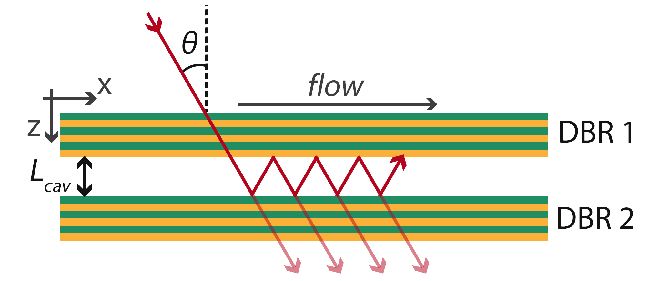
\includegraphics[width=\textwidth]{chap_theory/fig/cavity_geometry.pdf}
    \caption{Photon in a planar microcavity}
    \label{fig:cavity_geometry}
\end{figure}

\textbf{Planar microcavity parameters:}
First, let us consider an electromagnetic field incident at an angle $\theta$ on a planar microcavity made with two mirrors with reflectivities $R_1$ and $R_2$, separated by a distance $L$. The z-axis is normal to the mirrors as shown in \autoref{fig:cavity_geometry}. The phase shift acquired during a single round trip in the cavity is $\Delta \phi (\theta)=2nk_0L\cos(\theta)$, with $n$ the refractive index of the medium and $k_0=2\pi/\lambda$ the wave vector of the field in vacuum. The interference between the multiple reflections sets the resonance condition of the cavity, and the transmission of the field can be written as:

\begin{equation}
    T(\theta)=\frac{R_1R_2}{1+R_1R_2-\sqrt{R_1R_2}\cos(\Delta \phi(\theta)/2)}
    \label{eq:transmission_theta}
\end{equation}

\noindent From this, one can define the decay rate of the field oscillation known as the quality factor:
\begin{equation}
    Q=\frac{\omega_\gamma}{\Delta \omega_\gamma}
    \label{eq:Q}
\end{equation}
with $\omega_\gamma$ the resonance frequency of the cavity and $\Delta \omega_\gamma$ the linewidth of the resonance, which sets the lifetime of the photon in the cavity through $\tau_\gamma=1/\Delta \omega_\gamma$ and depends on the mirrors' reflectivities. Another important parameter describing the cavity is its frequency resolution, which is encoded in the cavity finesse through:

\begin{equation}
    \mathcal{F}=\pi \frac{\Delta \omega_\gamma}{\delta \omega_\gamma} = \pi \frac{\sqrt{R_1R_2}}{1-R_1R_2}
    \label{eq:F}
\end{equation}

where $\Delta \omega_\gamma$ is the Free Spectral Range (FSR) representing the frequency difference between two successive longitudinal modes of the cavity. To achieve strong coupling with the nonlinear medium, the photon needs to stay trapped in the cavity long enough to interact with the medium. In other words, the quality factor of the cavity must be very high, which means using mirrors with high reflectivities. This can be achieved with Distributed Bragg Reflectors (DBR) mirrors.

\begin{figure}[h]
    \centering
    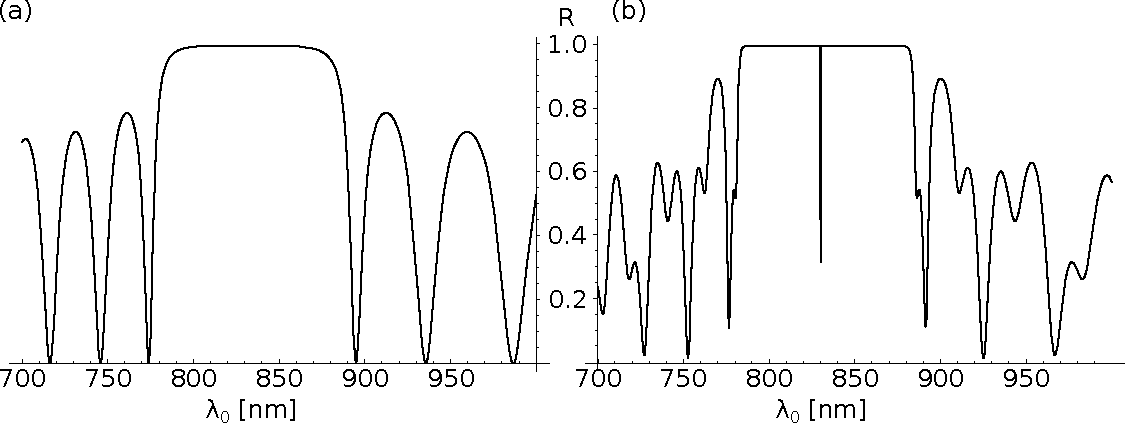
\includegraphics[width=1\linewidth]{chap_theory/fig/DBR.pdf}
    \caption{\textbf{DBR and Fabry-Perot cavity reflectivity.} \textbf{(a)} Reflectivity $R$ of a Bragg mirror of 20 pairs of Ga$_{0.9}$Al$_{0.1}$As/AlAs, illuminated at normal incidence for different wavelengths $\lambda$. The DBR has a reflectivity close to 1 over a large range of wavelengths called the stop-band, centered on $\lambda_0$ = 836 nm by tuning the thickness of each of the mirror layers. \textbf{(b)} Corresponding reflectivity of the optical cavity built from the facing of two DBR mirrors identical to that in (a) and separated by a distance $L_{\mathrm{cav}} = 2\lambda_0 / n_{\mathrm{cav}}$, leading to the appearance of a very narrow resonance at $\lambda_0$. Adapted from ??.}
    \label{fig:DBR}
\end{figure}

\textbf{Distributed Bragg Reflectors.} These reflectors consist of a series of N alternating layers composed of two materials with different refractive indices $n_1<n_2$. This configuration causes partial reflection of the electromagnetic field at each of the N interfaces, resulting in a very high overall reflection coefficient, $R$, which is expressed as follows:

\begin{equation}
    R = \left[  \dfrac{(n_2/n_1)^{2N} - n_f/n_0}{(n_2/n_1)^{2N} + n_f/n_0} \right]^2,
\end{equation}

with $n_0$ and $n_f$ representing the refractive indices of the media before and after the mirrors. \autoref{fig:DBR} illustrates the evolution of $R$ in relation to the wavelength of the electromagnetic field for one DBR mirror used in our system. This mirror is constructed with 20 pairs of $\text{Ga}_{0.9}\text{Al}_{0.1}\text{As}/\text{AlAs}$ layers, having refractive indices $n_2 = 3.48$ and $n_1 = 2.95$ respectively. The reflection coefficient $R$ is 0.9985 across a broad wavelength range, known as the stop-band, centered around a wavelength of $\lambda_0 = 836$ nm. This central wavelength is achieved by setting the thickness of the layers to $d_{1,2} = \lambda_0 / 4n_{1,2}$. The microcavity used in the experiments is built by facing two of those DBR mirrors separated by a distance $L_{\mathrm{cav}}=3\lambda_0/2n_{\mathrm{cav}}$, giving rise to a very narrow resonance at $\lambda_0$ with three field antinodes within the cavity. The parameters of the cavity are summarized in \autoref{DBR_params}.

\begin{center}
    \begin{tabular}{ |p{1.5cm}|p{1.5cm}|p{1.5cm}|p{1.5cm}|p{1.5cm}|p{1.5cm}|}
    \hline
    \multicolumn{6}{|c|}{Fabry-Perot cavity parameters} \\
    \hline
    \hline
    $R_1$ & $R_2$ & $n_1$ & $n_2$ & $n_{cav}$ & $\lambda_0$ (nm) \\
    \hline
    0.9992  &  0.9985 & 2.95 & 3.48 & 3.54 & 836\\
    \hline
    \label{DBR_params}
    \end{tabular}
\end{center}

With the above-described DBR, the cavity has a finesse $\mathcal{F}=2850$ from which we can infer the photon lifetime:
\begin{equation}
    \delta \omega_{\gamma} = \dfrac{\Delta \omega_{\gamma}}{\mathcal{F}} = \dfrac{c}{n_{\mathrm{cav}} L_{\mathrm{eff}}} \dfrac{1-R}{\sqrt{R}},
\end{equation}
where $L_{\mathrm{eff}}= L_{\mathrm{cav}}+L_{\mathrm{bragg}}$ is the effective length of the sample taking into account the penetration of the field in the mirrors.
\begin{equation}
    L_{\mathrm{Bragg}} = \dfrac{\lambda_0}{2} \dfrac{n_1 n_2}{n_{\mathrm{cav}} (n_2 - n_1)}
\end{equation}
which gives $\tau_{\gamma} = \frac{1}{\delta \omega_{\gamma} }= 5$ ps.

\bigskip\noindent
\textbf{Transverse dynamics of the photon.} The energy of the photon within the sample can be written as:
\begin{equation}
    E_\gamma = \dfrac{\hbar c}{n_{\mathrm{cav}}} \sqrt{k_x^2 + k_y^2 + k_z^2}.
\label{free_space_photon}
\end{equation}
The resonance condition of the cavity fixes the photon wavevector along the z component. 

\begin{equation}
    k_z = \dfrac{2\pi n_{\mathrm{cav}}}{\lambda_0}.
    \label{eq:kz}
\end{equation}
In the paraxial approximation $k_x,k_y \ll k_z$, one can expand \eqref{free_space_photon} in terms of $\frac{||\bm{k_{\parallel}}||}{||\bm{k_z}||}$ as:
\begin{equation}
    E_\gamma = \dfrac{\hbar c}{n_{\mathrm{cav}}} \sqrt{k_z^2 + k_{\parallel}^2} = E_0 \left( 1 + (\hbar k_{\parallel })^2 \dfrac{c ^2}{2(n_{\mathrm{cav}} E_0)^2} \right).
    \label{eq:paraxial_photon}
\end{equation}
where $\bm{k_{\parallel}}=\bm{k_x}+\bm{k_y}$ is the wavevector in the transverse plane and $E_0=hc/\lambda_0$ is the photon energy in free space. We can identify the effective mass of the photon by writing \eqref{eq:paraxial_photon} with the usual form of the kinetic energy of a massive particle:

\begin{equation}
    E_\gamma = E_0 + \dfrac{p_{\parallel}^2}{2m_{\gamma}}  
    \label{eq:photon_mass}
\end{equation}
where we identify $m_{\gamma} = \dfrac{\hbar n_{\mathrm{cav}}^2}{\lambda_0 c}$ which is inversely proportional to the second derivative of the energy with respect to $k_{\parallel}$:

\begin{equation}
    \dfrac{1}{m_{\gamma}} = \dfrac{1}{\hbar^2}\dfrac{\partial^2 E_{\gamma}}{\partial k_{\parallel}^2}
    \label{eq:mass}
\end{equation}

\noindent\textbf{Momentum conservation:}
we mentioned the necessity to have a high quality factor to later achieve strong coupling. One could then ask why do we stick to planar designs, which are generally not the best solution to get a high Q factor since they are known to be unstable except for plane waves. The answer lies in the calculation just above. Indeed, the advantage of having a planar design is the translational invariance in the xy plane, which brings $\bm{k_{\parallel}}$ conservation. As a consequence, if one shines a laser with a given $\bm{k_{\parallel}}$, light will behave in the cavity as a massive particle moving at velocity $v_\gamma=\hbar \bm{k_{\parallel}}/m_\gamma$. In the picture of creating a fluid whose flow is controlled, the planar design then appears as a wise choice.

\bigskip\noindent

\noindent\textbf{A direct link between incidence angle and in plane momentum $k_{\parallel}$:}
as shown in \autoref{fig:cavity_geometry} the incidence angle $\theta= (\theta_x, \theta_y)$ of the incoming field is related to the in-plane momentum $k_{\parallel}$ as :

\begin{equation}
    k_{x} = k_0 \sin(\theta_x) \\
    k_{y} = k_0 \sin(\theta_y)
    \label{eq:kpar}
\end{equation}

Controlling the in plane momentum of photons and latter of polaritons then boils down to control the local incidence angle of the field, in other words, the transverse phase of the incoming beam. This is a crucial point for the experiments as it allows to control the flow of the fluid by changing the laser phase.

\bigskip\noindent
\textbf{Conclusion:}
This section revealed how trapping light in a planar microcavity grants it effective mass and lifetime. The next section will explore the semiconducting media that can be inserted into these cavities, especially the bound electron-hole pairs called excitons that can be addressed by the trapped light.


\section{Excitons in Semiconductors}

\subsection{Band theory in brief}

Applying the Schrodinger equation to an atom reveals that the electrons energies can only take discrete values. However, N atoms sufficiently close to each other interact which lift the degeneracy and 
turns each energy state in a set of N separated levels (see \autoref{fig:band_theory}). 
Within a solid material, the density is so high (typicaly $10^{22}$ atoms per cm$^3$) that the spacing between energy levels tends to zero forming a continuous band of energy. 
The electrons fill the band from the lowest energy level up to the Fermi energy. The Fermi energy is the energy of the highest occupied state at zero temperature. 
The band structure of a material is then defined by the energy of the valence band, the conduction band and the band gap between them. The valence band is the highest energy band that is fully occupied at zero temperature, while the conduction band is the lowest energy band that is empty at zero temperature. The band gap is the energy difference between the conduction band and the valence band. 
Determining if a material is a metal, a semiconductor or an insulator is then a matter of comparing the band gap to the Fermi energy.
For metals the conduction band and the valence band overlap, any electric potential difference puts then the electron into motion and create a current. For insulators and semiconducting materials the Fermi energy is in the band gap. For insulators the band gap is typicaly $\sim 3 \ \mathrm{eV}$ making the promotion of an electron to the conduction band highly energy demanding. 
Finally, the semiconductors gap energy is accessible with photons in the visible domain making these materials perfect candidates for controlled light-matter interactions.

\begin{figure}[h]
    \centering
    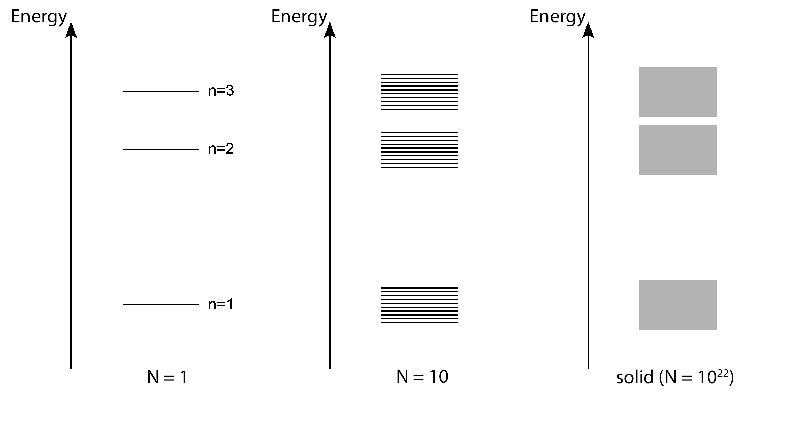
\includegraphics[width=1\linewidth]{chap_theory/fig/band_theory.pdf}
    \caption{\textbf{Energy levels of a set of N atoms.} As N increase the spacing between two successive levels tends to zero and eventually form a continuous band of energy.}
    \label{fig:band_theory}
\end{figure}

\subsection{Band structure of semiconductors}

Finding the exact band structure of a material can be done by solving the Schrodinger equation for an electron in periodic potential.
 The Bloch theorem states that the wave function of such an electron can be written as a plane wave modulated by a periodic function. The periodic function is then expanded in a Fourier series and the Schrodinger equation is solved for each Fourier component. 
 The exact band structure can be rather complicated but a simplified version can be obtained by considering the effective mass approximation \cite{kittel_introduction_2005}. In this picture, the dispersion relation of the electron in the material is typically represented in \autoref{fig:Direct_gap_disp}.
In this case the minimum of the conduction band and the maximum of the valence band are located at the same point in the Brillouin zone. The material is then said to have a direct band gap.
\begin{figure}[h]
    \centering
    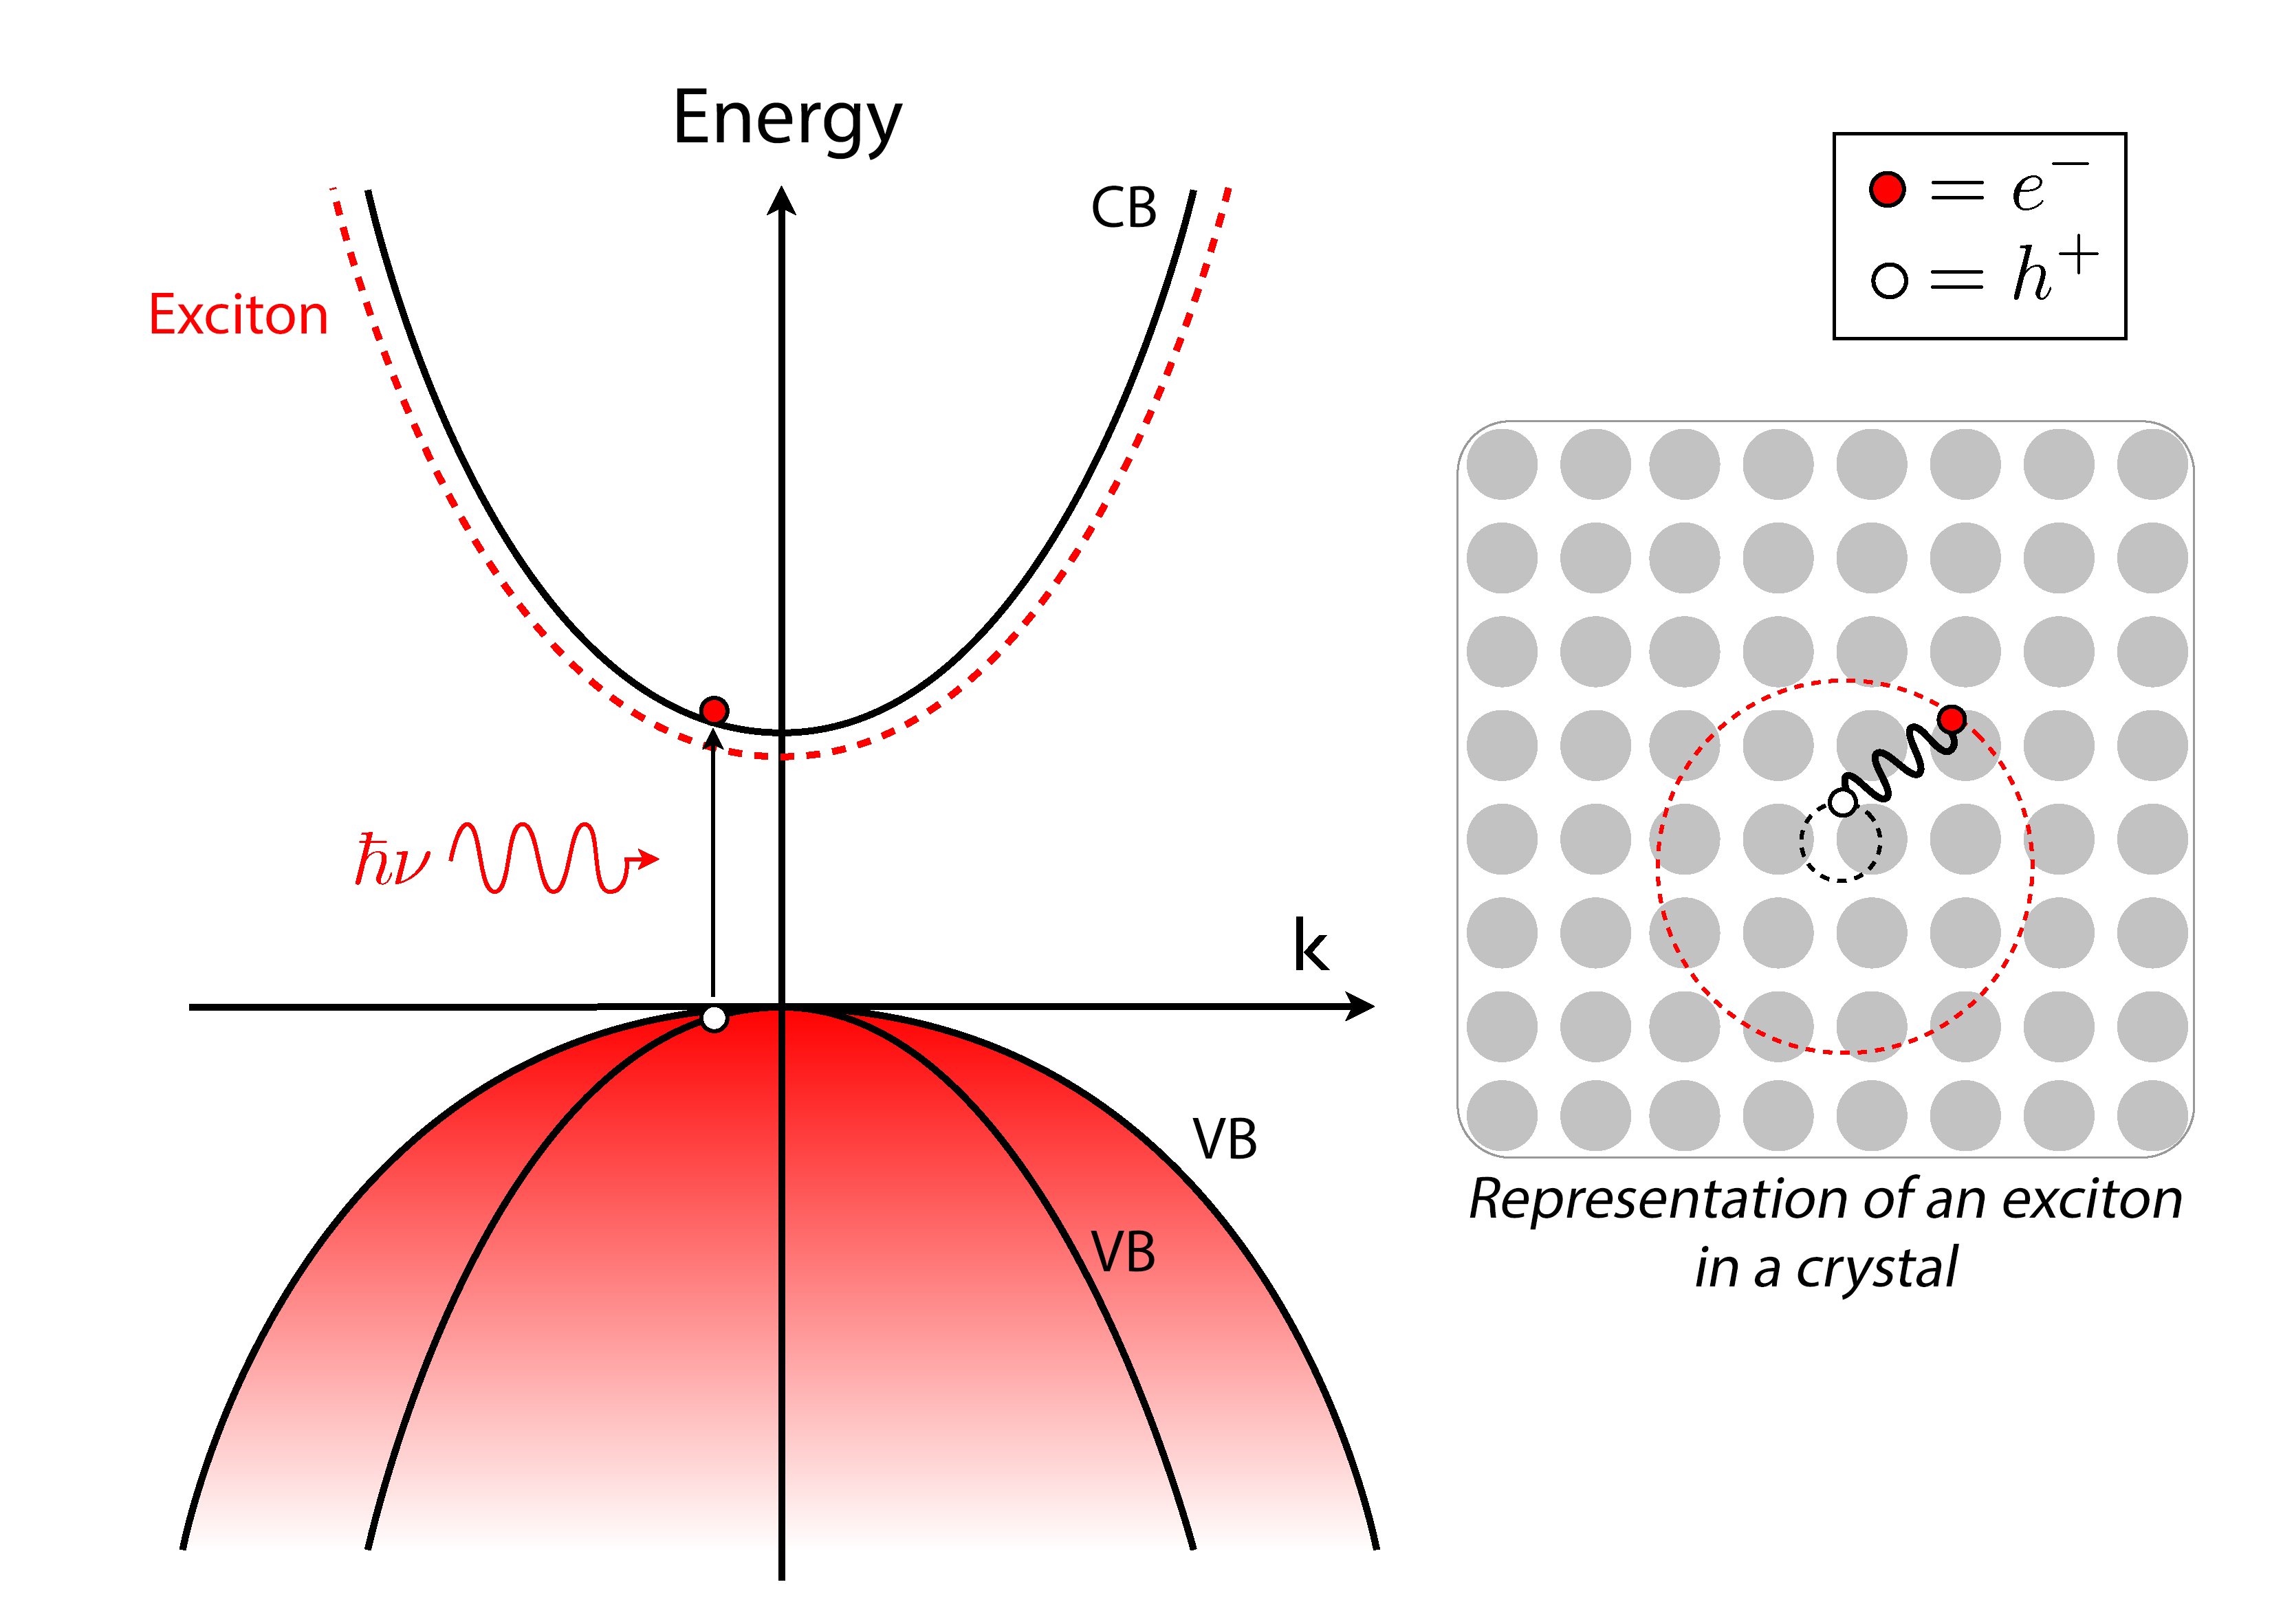
\includegraphics[width=0.8\linewidth]{chap_theory/fig/DirectGapDisp.png}
    \caption{\textbf{Band structure of a direct gap semiconductor.} The black solid line represent the conduction and valence band in a bulk semiconductor. The red dashed lines represent the dispersion relation of an exciton. The filling of the valence band by electrons is represented by the shaded red color.}
    \label{fig:Direct_gap_disp}
\end{figure}


\subsection{Exciton phenomenological approach}

\label{sub:exciton}

As shown in \autoref{fig:Direct_gap_disp} shinning a photon whose energy exceed the gap energy can promote an electron from the valence band to the conduction band through the absorption of a photon. 
The disappearance of the electron in the valence band can be described equivalently as the creation of a virtual particle of opposite charge called hole \cite{Combescot_cooper_excitons_2015}.
 If one scan shine a laser on a semiconductor and ramp up its frequency a narrow absorption peak is observed below the gap energy.  The presence of this peak originate from the coulombic interaction between the created electron and the hole creating a bound state of the material. In terms of energy it's as if the gap energy is reduced by the binding energy of the exciton and the electron lies in a virtual band below the conduction band as represented by the red dashed lines in \autoref{fig:Direct_gap_disp}.
 The exciton energy can then be written as : 

\begin{equation}
    E_{X} = E_g - E_b + \frac{\hbar^2 K^2}{2m_{X}}
\end{equation}

where $E_g$ is the gap energy, $E_b$ the binding energy,  $\hbar \vec{K}$ is the exciton momentum defined as the electron-hole pair center of mass momentum and $m_{X}$ the exciton effective mass which is the sum of the electron and hole effective mass.
Since $E_b$ is the interaction energy between a electron and a hole it is, as we will se in the next section, very similar to the Rydberg energy series of the hydrogen atom, the hole playing the role of the proton. As a consequence, the same electronic structure exist for the exciton : 1s, 2s, 2p, etc state can be observed in the absorption spectrum of the material.
However, the hole is quite different from the proton in the sense that it's actually a collective excitation of all the valence band electrons. Furthermore the exciton is a weakly bound state as the binding energy is typically a few meV. In GaAs or AlGaAs heterostructures which are the materials used in the present work $E_b$ is around 4 meV due to their high dielectric constant $\epsilon_r \sim 12$.
In these kind of samples, excitonic resonances can only be observed at cryogenic temperatures since the binding needs to exceeds the thermal energy $k_B T$ in order to survive the thermal fluctuations. For the above mentionned structures we obtain the condition $T<10$ K for excitons stability.
Another important exciton characteristic is their huge Bohr Radius $a_X= \frac{\epsilon_r \hbar^2}{m_X e^2}= 11.6 \ \mathrm{nm}$ in GaAs which  is much larger then the typical size of a unit crystalline cell $a_0 = 5.65 \SI{1}{\angstrom}$. This means that the exciton wavefunction is delocalized over many unit cells. Such excitons, are called Wannier-Mott and constrast with Frenkel excitons which are localized on a single unit cell and are typically found in organic materials.
 \bigskip\noindent

\subsection{Electron-hole interactions and exciton formation}

Excitons were said to be made of an electron and a hole bound by Coulombic interactions. However, all the interactions in the material are ultimately mediated by valence and conduction band electrons. The rising
of a bound state in such a material is therefore not obvious. In other words moving from a conduction-valence band electrons to a electron-hole picture is not trivial and reveals interesting
feature about the electron-hole interactions that will at the end enable exciton formation. In this section we will first describe all the possible interactions between the electrons of the semiconductor before showing how they can be recasted in terms of electron-hole interactions.

\bigskip
\subsubsection{Electron scattering in semiconductors}
\begin{figure}[h]
    \centering
    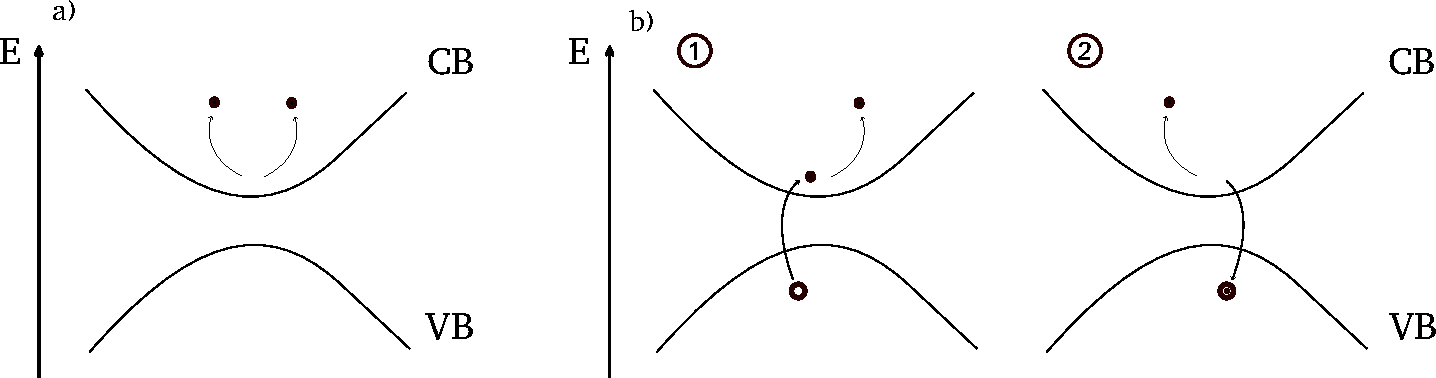
\includegraphics[width=1\linewidth]{chap_theory/fig/intra-inter-band-processes.pdf}
    \caption{\textbf{Drawing representing the scattering between two conduction band electrons.} a) Direct intraband scattering. Filled black dots represent conduction band electrons. b) Two steps scattering involving an electron-hole exchange or creation an annihilation of an exciton, referred as interband scattering.
    The empty black circle represent a valence band hole while the same circle with a small black dot inside stands for a valence band hole filled with an electron which is equivalent to a valence electron. a) and b) share the same
     final state which is a full valence band and two scattered conduction band electrons. Drawing inspired from \cite{Combescot_cooper_excitons_2015}.}
    \label{fig:inter-intra-scat}
\end{figure}


\textbf{Intraband scattering :}
to start with let's consider the direct scattering between two conduction band electrons as presented in \autoref{fig:inter-intra-scat} a). This simple process is referred as intraband scattering since each electron stays in its own band. In the small momentum limit $\mathrm{\textbf{q}}\to 0$ it yields a potential of the form:

\begin{equation}
    V_{\textbf{q}} \simeq \dfrac{4\pi e^2}{L^3 q^2}
\end{equation}
 
\noindent in a sample of size L. This form of potential holds also for the scattering between two valence electrons or between a valence and a conduction band electron that stay in their respective bands.

\bigskip

\textbf{Interband scattering :}
processes in which one or two electrons change band are also possible and are referred as interband scattering. In the case of a single 
interband jump the potential reads $(\frac{q}{\kappa})V_{\textbf{q}}= \dfrac{4\pi e^2}{L^3 q \kappa}$ where $\kappa$ is a dimensionnal factor that depends on the material. It then behaves as $1/q$. When both electrons change band the potential is then $(\frac{q}{\kappa})^2V_{\textbf{q}}$ proportionnal to $q^0$
and thus remaining finite when $q\to 0$. Remarkably, in both the single and two interband jump scenarios, the number of electrons in each band changes by one and two, respectively, making these transitions less likely to occur compared to number-conserving processes.

\bigskip
Indeed, in second order perturbation theory the transition amplitude between an initial state $\ket{i}$ and a final state $\ket{f}$ may be written as :

\begin{equation}
    \Gamma_{i\to f}^{(2)} = \dfrac{2\pi}{\hbar} \bigg \vert \sum_{m} \dfrac{\bra{f}V_q\ket{m}\bra{m}V_q\ket{i}}{E_i - E_m}\bigg \vert^2 \delta(E_f - E_i)
    \label{eq:transition_amplitude}
\end{equation}

\noindent Whenever an electron undergo a band jump the energy cost is of the order of the band gap $E_f - E_i \simeq E_g$. As a consequence the corresponding transition amplitude gets reduced by a factor $\frac{1}{E_g}$ and appears to be negligible.
 However a direct intraband scattering can happen in several interband jumps that will dress the direct Coulomb scattering as shown in \autoref{fig:inter-intra-scat} b) for the case of two jumps. When summing over all possible intermediate state as is \eqref{eq:transition_amplitude} we end up with the same potential as the direct intraband scattering but reduced by dielectric constant factor $\epsilon_{sc}$ that depend on the material.

 
\bigskip




To clarify this idea let us now consider the scattering between a conduction and a valence band electron. 
The same scattering process can also occur in two steps. First, a conduction band electron is scattered in its band while a valence band electron is promoted to the conduction band. Since an electron changes band it brings a potential $V_q(q/\kappa)$. Secondly, 
 the excited electron goes back to the valence band while a valence band electron is scattered in its band yielding again a potential $V_q(q/\kappa)$. This two steps interaction end up with the same initial and final states than direct intraband scattering and the number of electrons in each band is conserved.  
In terms of energy, the two scatterings behaving as $1/q$ potentials the overall potential behaves also as $1/q^2$ but with an additionnal $1/E_{g}$ factor coming from the intermediate interband jumps. More specifically the two steps contribution is : $\left( 4\pi e^2/L^3q^2 \right)\left[ (e^2/L^3\kappa^2)/E_{g}\right]$.  

\bigskip
It is also possible to make it a three steps scattering by adding an intermediate interband exchange after the first step : the previously excited conduction band electron returns to the valence band while a valence band electron is promoted to the conduction band. 
Moe explicitly the process is as follows : 

\begin{itemize}
    \item \textbf{Step 1 :} a valence band electron is promoted to the conduction band while a conduction bandis scattered in its band. The potential reads $V_q(q/\kappa) \propto \frac{1}{q}$ and the energy cost is of the order of $E_g$.
    \item \textbf{Step 2 :} the previously excited conduction band electron returns to the valence band while another valence band electron is excited to the conduction band. The potential read $V_q(q/\kappa)^2 \propto q$ and the energy cost is of the order of $2E_g$.
    \item \textbf{Step 3 :} the excited electron goes back to the valence band while a valence band electron is scattered in its band. The potential read again $V_q(q/\kappa) \propto \frac{1}{q}$ and the energy cost is of the order of $E_g$.
\end{itemize}

\noindent The total energy budget is then : $\left( 4\pi e^2/L^3q^2 \right)\left[ (e^2/L^3\kappa^2)/E_{g}\right]^2$. Remarkably, one might expect the overall potential to scale as $1/E_g^3$  since each step requires at least one electron to change band. However, the structure of perturbation theory ensures that the total energy denominator accounts for the number of coupled interband transitions, rather than treating each step independently. 
Step 2 effectively "couples" the transitions in such a way that two energy denominators are introduced, rather than three independent ones, which explains the 
$1/E_g^2$ dependence. This coupling reflects the fact that intermediate states are shared between adjacent steps in the perturbative sequence.
\bigskip 


\begin{figure}[h]
    \centering
    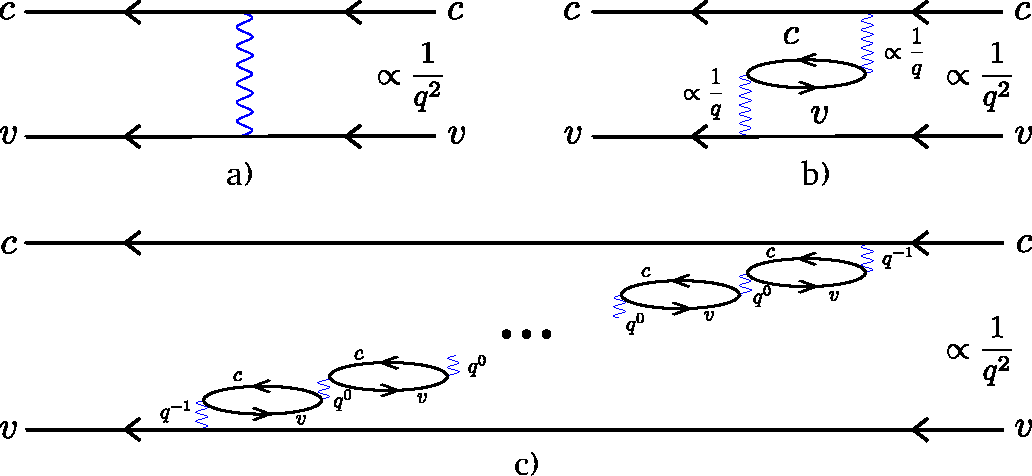
\includegraphics[width=1\linewidth]{chap_theory/fig/intra_band_dressed_bubbles.pdf}
    \caption{\textbf{Feynman diagrams representing an intraband scattering between a conduction and a valence band electron.} a) Direct intraband scattering. The blue wavy lines represent the Coulomb interaction that make the electrons to change states. b) Two steps scattering involving an intermediate interband exchange that is represented by the bubble in the middle.
    c) Multiple steps scattering involving several interband exchanges represented by the numerous bubbles.
    Drawing inspired from \cite{Combescot_cooper_excitons_2015}.}
    \label{fig:intra_bubbles}
\end{figure}

Finally, the number of intermediate states can be arbitrarily increased by adding 'bubbles' of exchange interaction, as illustrated in the Feynman diagram in \autoref{fig:intra_bubbles} b). Each pair of adjacent bubbles represents an interband interaction similar to the one described in Step 2 above. While it conserves the number of electrons in each band, it involves two interband jumps. 
The interaction between two bubbles is then $\propto q^0$ and is finite in the small momentum limit.
By summing the contributions of processes with all possible numbers of bubbles, we obtain an effective Coulomb potential:

\begin{equation}
    V_q = \dfrac{4\pi e^2}{L^3q^2\epsilon_{sc}}
    \label{eq:effective_potential_intraband_scattering}
\end{equation}

where $\epsilon_{sc}$ is a dielectric constant stemming from the infinite sum over the number of bubbles. The discussion that we just made also holds for the intraband scattering between two conduction band electrons or two valence band electrons.
Indeed, it graphically boils down two change the letter of the bands in the Feynman diagrams of \autoref{fig:intra_bubbles} which doesn't change the overall energy budget of the process. Consequently, the potential \eqref{eq:effective_potential_intraband_scattering} is valid for all intraband scattering processes.
Based on the previous discussion we restrict the Coulomb potential that describe any scattering process to interactions that conserve the number of particle in each band, namely the intraband scattering potential between conduction and valence band electrons derived above.
The general form of the potential is then in second quantization :
\begin{equation}
    V_{coul}\simeq \dfrac{1}{2}\sum_{\textbf{q}\neq 0}\Vintra\sum_{\mathbf{k_{1}, k_{2}}}\sum_{\mathrm{i_1,i_2}} a^{\dagger}_{\mathrm{i_{1}},\mathbf{k_1+q}}a^{\dagger}_{\mathrm{i_{2}},\mathbf{k_2-q}}a_{\mathrm{i_{2}},\mathbf{k_2}}a_{\mathrm{i_{1}},\mathbf{k_1}}
\end{equation}

\noindent where $\mathrm{i_1,i_2} \in (c,v)$. The creation operators $a^{\dagger}_{c,\mathbf{k}}$ and $a^{\dagger}_{v,\mathbf{k}}$ create respectively a conduction and a valence band electron with momentum $\mathbf{k}$.
The $\textbf{q}=0$ contribution is not included and treated separately by the wise choice of an average electron-electron potential $V_{e-e}$ that cancels it. More details can be found in the Appendix of \cite{Combescot_cooper_excitons_2015}.
It is worth noting that, in the conduction-valence electron framework, all intraband interactions are identical and repulsive. From this it is not obvious how a bound state like an exciton can arise in the material. However, as we will see in the next section, transitioning to the electron-hole description transforms one of these scattering interactions into an attractive interaction.
 This feature is central to the energy splitting between two types of excitons: bright excitons, which couple to light, and dark excitons, which do not.

\subsubsection{From the conduction-valence electrons to electron-hole picture}

\label{sub:electron_hole_picture}
So far we described the scattering processs within the semiconductor using valence and conduction electrons. However, the exciton results form the binding between a conduction band electron and the absence of a valence band electron that we usually describe as a hole.
While the conduction electron description stays the same, moving from one picture to the other require to define the hole creation operator that account for the removal of a valence band electron or equivalently the creation of a hole in the valence band.


\begin{subequations}
    \label{eq:hole_creation_operators} % Étiquette pour le groupe d'équations
    \begin{align}
        a^{\dagger}_{c,\mathbf{k}} &= a_{\mathbf{k}},\label{eq:electron_operator} \\
        a_{v,\mathbf{k}} &= h^{\dagger}_{\mathbf{-k}},\label{eq:hole_operator}
    \end{align}
\end{subequations}


\noindent where $h^{\dagger}_{\mathbf{-k}}$ creates a hole in the valence band with momentum $-\mathbf{k}$. The - sign 
is imposed by energy and momentum conservation laws. When we substitute the full valence band with a missing electron with momentum $\mathbf{k_v}$ by a hole, the hole needs to have opposite charge $+|e|$, momentum $\mathbf{k_h}=-\mathbf{k_v}$ and energy $E_h(\mathbf{k})=-E_v(\mathbf{k})$ to account for the "absence" of the valence electron. 
In the small momentum limit we have $E_v(\mathbf{k}) = E_{v_0}+ \frac{\hbar^2 k_v^2}{2m_v}$ with $m_v$ the valence electron effective mass that is negative as visible in \autoref{fig:Direct_gap_disp}.
The constraint on the energy $E_h = -E_v$ then imposes $ \frac{\hbar^2 k_h^2}{2m_h} = - \frac{\hbar^2 k_v^2}{2m_v}$ making the effective mass of the hole positive. Its charge and mass being positive it can then undergo attractive interactions 
with a conduction band electron and eventually form an exciton. We already see how describing the valence band with hole instead of electrons can predict the formation of bound state.
Let us now look how this feature arise from a microscopic point of view. The full crystal hamiltonian is :

\begin{equation}
    \Ham =  \Ham_0 + V_{coul}
    \label{eq:crystal_hamiltonian}
\end{equation}

\noindent with $\Ham_0$ the free electron hamiltonian and $V_{coul}$ the Coulomb interaction between electrons. The free electron hamiltonian reads :

\begin{equation}
    \Ham_0 = \sum_{\mathbf{k}} E_c(\mathbf{k}) a^{\dagger}_{c,\mathbf{k}}a_{c,\mathbf{k}}+\sum_{\mathbf{k}} E_v(\mathbf{k}) a^{\dagger}_{v,\mathbf{k}}a_{v,\mathbf{k}}
    \label{eq:free_electron_hamiltonian}
\end{equation}

\noindent where $E_c(\mathbf{k})$ and $E_v(\mathbf{k})$ are the conduction and valence band energies respectively. The Coulomb interactions part can be decomposed in the following way :

\begin{equation}
    V_{coul} = V_{cc} + V_{vv} + V_{cv}
    \label{eq:coulomb_interaction}
\end{equation}
Using the newly defined operators together with fermionic commutation relation $a^{\dagger}_{i,\textbf{k}}a_{i,\textbf{k}}= 1-a_{i,\textbf{k}}a^{\dagger}_{i,\textbf{k}}  $ the different scattering potentials are modified as we now show. 

\begin{itemize}
    \item The one body hamiltonian reads : 
    \begin{equation}
    \Ham_0 = \sum_{\veck}E_v(\veck)+ \sum_{\veck}E_c(\veck) a^{\dagger}_{\veck}a_{\veck} + \sum_{\veck}-E_v(\veck) h^{\dagger}_{\veck}h_{\veck}.
    \end{equation}

    \item The scattering between two conduction band electron is the same as before :
    \begin{equation}
    V_{cc} = \dfrac{1}{2}\sum_{\textbf{q}\neq 0}V_{\mathbf{q}} \sum_{\mathbf{k_{1}, k_{2}}} a^{\dagger}_{\mathbf{k_1+q}}a^{\dagger}_{\mathbf{k_2-q}}a_{\mathbf{k_2}}a_{\mathbf{k_1}} \equiv V_{ee}
    \label{eq:cc_interaction}
    \end{equation}

    \item The scattering between two valence band electrons splits into three terms :
    \begin{equation}
    V_{vv}=-\dfrac{N_v}{2}\sum_{\veck \neq 0}V_{\veck} + \sum_{\veck}\hkdag\hk\sum_{\veck'\neq \veck}V_{\veck'-\veck}+V_{hh}.
    \label{eq:vv_interaction}
    \end{equation}

    The first term is constant and account for repulsive exchange interaction between all valence electrons. The second term comes from the scattering between a valence electron with wavevector $\veck$ and all the other valence electrons.
    It adds a shift to the hole kinetic energy $E_h = -E_v$ that appears in the one body hamiltonian $\Ham_0$. 
     The last term is the hole-hole interaction that is repulsive and is the same as the valence electron-electron interaction with opposite wavevectors : 
    \begin{equation}
    V_{hh} = \dfrac{1}{2}\sum_{\textbf{q}\neq 0}V_{\mathbf{q}} \sum_{\mathbf{k_{1}, k_{2}}} h^{\dagger}_{\mathbf{k_1+q}}h^{\dagger}_{\mathbf{k_2-q}}h_{\mathbf{k_2}}h_{\mathbf{k_1}} 
    \label{eq:hh_interaction}
    \end{equation}

    \item Finally, scattering between a conduction and a valence band electron is :
    \begin{equation}
    \label{eq:cv_interaction_in_cv_picture}
    V_{cv} = \sum_{\textbf{q}\neq 0}V_{\mathbf{q}} \sum_{\mathbf{k_{1}, k_{2}}} a^{\dagger}_{c,\mathbf{k_1+q}}a^{\dagger}_{v,\mathbf{k_2-q}}a_{v,\mathbf{k_2}}a_{c,\mathbf{k_1}}.
    \end{equation}
    Using that for non zero momentum transfer $[a^{\dagger}_{v,\mathbf{k_2-q}}, a_{v,\mathbf{k_2}}] = 0$ and introducing $\mathbf{k_2'} = -(\mathbf{k_2-q})$ the potentials in terms of electron-hole reads :
    \begin{equation}
        V_{cv} = -\sum_{\textbf{q}\neq 0}V_{\mathbf{q}} \sum_{\mathbf{k_{1}, k_{2}'}} a^{\dagger}_{\mathbf{k_1+q}}h^{\dagger}_{\mathbf{k_2'-q}}h_{\mathbf{k_2'}}a_{\mathbf{k_1}} \equiv V_{eh}.
    \label{eq:eh-interaction}
    \end{equation}

\end{itemize}
The latter require a special attention since it exhibits an attractive interaction and reveals the possibility of excitons formation which was not obvious in the conduction-valence electron picture.
\bigskip

\noindent \large \textbf{Spin conservation in electron scattering } \normalsize
\bigskip


Scatterings processes mediated by the Coulomb interactions conserve the spin of the electron for both interband and intraband scatterings. As a consequence,
the interactions between electons and holes that we just exhibited are also spin preserving. The latter has important consequences to determine
selection rules when looking at optical excitation of an electron-hole pair. 

\bigskip

\indent So far we demonstrated that replacing the full valence band by a hole looks quite convenient since it allow to forget about all the valence band electrons and exhibits the possibility of bound state formation. However, it must be done with caution
since the remaining valence band electrons undergo the many intraband scattering processes described in the section and reduce the effective Coulombic intraband interaction by 
a factor $1/\epsilon_{sc}$. Remarkably, the intraband scatterings between valence and conduction band electrons $V_{cv}$ are at the origin of the attractive electron-hole interactions while valence-valence interactions are responsible for the shift in the hole kinetic energy as expressed by \autoref{eq:vv_interaction}.
Let us now explain how the aforementioned electron-hole attractive interactions can lead to exciton formation.

\subsubsection{The electron-hole hamiltonian}
\label{e-h_hamiltonian}

If we restrict the previous description to a one pair subspace namely to the interactions between a single electron and a single hole, electron-electron and hole-hole
interactions can be safely dropped since they require two holes or electrons. The one pair hamiltonian then reads : 


\begin{equation}
    \begin{align}
    \Ham_{eh} &= \Ham_e + \Ham_h + V_{eh}, \\
              &= \sum_{\veck}E_c(\veck) a^{\dagger}_{\veck}a_{\veck} + \sum_{\veck}E_h(\veck) h^{\dagger}_{\veck}h_{\veck} - \sum_{\textbf{q}\neq 0}V_{\mathbf{q}} \sum_{\mathbf{k_{1}, k_{2}}} a^{\dagger}_{\mathbf{k_1+q}}h^{\dagger}_{\mathbf{k_2-q}}h_{\mathbf{k_2}}a_{\mathbf{k_1}}.
    \label{eq:electron_hole_hamiltonian}
    \end{align}
\end{equation}
Wannier exciton are the solutions $\ket{x}$ of the eigenproblem :
\begin{equation}
    (\Ham_e + \Ham_h + V_{eh})\ket{i}= E_i\ket{i}
    \label{eq:exciton_eigenproblem}
\end{equation}
with eigenvalue $E_i$.
At this level the hamiltionian is very general and describe two coupled harmonic oscillators. Without going into details, this problem can be solved by following the same procedure as in classical mechanics.
The core of the derivation consists in decoupling the two oscillators by introducing new coordinates that are the center of mass and relative coordinates. Since Coulombic interaction conserve momentum, the total momentum of the
electron-hole pair $k_e+k_h$ stays constant and is equal to the exciton center of mass momentum $\mathbf{Q}$. Namely, we define :

\begin{subequations}
    \begin{align}
        \mathbf{Q} &= \mathbf{k_e} + \mathbf{k_h}, \\
        \mathbf{q} &= \gamma_h\mathbf{k_e} - \gamma_e\mathbf{k_h},
    \end{align}
\end{subequations}
where $\gamma_e =1- \gamma_h= m_e/(m_e+m_h)$ is the reduced mass ratio and $\mathbf{q}$ is the relative motion momentum. We then define the creation operator that creates an exciton $\ket{x}$ in state $(\mathbf{Q_i}, \nu_i)$ in terms of electron and hole operators : 

\begin{equation}
    b^{\dagger}_{\mathbf{Q_i},\nu_i} =  \sum_{\mathbf{p}}f_{\mathbf{p}}^{\nu_i}a^{\dagger}_{\gamma_e\mathbf{Q_i}+\mathbf{p}}h^{\dagger}_{\mathbf{-p+\gamma_h\mathbf{Q_i}}}
\end{equation}
\bigskip
\noindent where $f_{\mathbf{p}}^{\nu_i} = \bra{\mathbf{p}}\ket{\nu_i}$ is the relative motion wave function. Let us show that the states $\ket{\nu_i}$ are the eigensolutions of a Hydrogen like problem $\nu_i$ being then related to the first quantum number of an electron orbitals. Injecting $\ket{x}= b^{\dagger}_{\mathbf{Q_i},\mathbf{q_i}}\ket{0}$, $\ket{0}$ being the vacuum state in 
\autoref{eq:exciton_eigenproblem} we obtain $\Ham_{eh}$ in a diagonal form :

\begin{equation}
    \begin{align}
    \Ham_{eh}b^{\dagger}_{\mathbf{Q_i,\nu_i}}\ket{0} = \sum_{\mathbf{p}}  \left\{\left(E_g + \dfrac{\mathbf{Q_x}^2}{2m_X} + \dfrac{\mathbf{p_x}^2}{2\mu_X} \right)f_{\mathbf{p}}^{\nu_i} - \sum_{\mathbf{q}\neq 0} V_\mathbf{q}f_{\mathbf{p-q}}^{\nu_i}\right\}a^{\dagger}_{\mathbf{p+\gamma_e\mathbf{Q_i}}}h^{\dagger}_{\mathbf{-p+\gamma_h\mathbf{Q_i}}}\ket{0}
    \end{align}
\end{equation}
whose eigenstates are $b^{\dagger}_{\mathbf{Q_i,\nu_i}}\ket{0}$ with energy $E_{X_i} = E_g + \frac{\mathbf{Q_i}^2}{2M_X} + E_{b}^i$ if and only if $f_{\mathbf{p}}^{\nu_i}$ are solution of the Hydrogen-like problem : 

\begin{equation}
    \dfrac{\mathbf{p}^2}{2\mu_X}f_{\mathbf{p}}^{\nu_i} -\sum_{\mathbf{q}\neq 0} V_\mathbf{q}f_{\mathbf{p-q}}^{\nu_i} = E_b^if_{\mathbf{p}}^{\nu_i}
    \label{eq:hydrogen_like_problem}
\end{equation}
 where $\mu_X^{-1}= m_e^{-1}+m_h^{-1}$ is the relative motion mass and $m_X = m_e+m_h$ the total mass. The exciton then appears as a bound state of the electron-hole pair with a binding energy $E_{b_i}$ whose center of mass 
 is delocalized as a plane wave with momentum $\mathbf{Q}$. The binding energies $E_b^i$ follows a Rydberg series $E_b^i = -\dfrac{R_X}{i^2} $ where $R_X$ is the Rydberg constant of the exciton as defined in \autoref{sub:exciton}
In the following section we will see how the excitons interact with light.

 \subsection{Exciton-photon interaction in bulk semiconductor:} 
 \label{sub:exciton_photon_interaction}
The creation of an exciton can be mediated by the absorption of a photon by the material. On the other the annihiliation of a exciton can lead to photon emission.
As a start we describe this interaction with an usual electron-photon Hamiltonian in first quantization:


\begin{equation}
    \Ham_{dip} = -e \dfrac{\mathbf{p_e} \cdot \mathbf{A}}{m_e},
\end{equation}

with $\mathbf{p_e}$ the momentum operator of the electron and $\mathbf{A}$ the potential vector of the electromagnetic field. Before going further let us have a look at what the symetries of this Hamiltonian imply based on the Noether theorem.

\begin{itemize}
    \item \textbf{Total momentum conservation :}  translational invariance of the system implies that the total momentum of the system is conserved. The absorption of a photon with momentum 
    $\hbar \vec{k_c}$ will create an exciton with the same momentum.
    \item  \textbf{Total angular momentum conservation :} rotational invariance of the system implies that the total angular momentum of the system is conserved along the interaction.
\end{itemize}

The second point raises the question of the possible values that the exciton angular momentum can assume. To answer this question we need to get back to its 
microscopic constitutive particles : a conduction band electron and a hole in the valence band. In usual semiconductors a conduction band electron has an orbital angular momentum ($L=0 , L_z=0$) while a valence band electron yields ($L=1 , L_z=(+1,0,-1)$) (see \cite{kittel_introduction_2005}).
Since $J_z = J_z + S_z$ and the electron spin is $S_z = \pm 1/2$ we obtain for the valence band $J_z^{v} = (3/2, 1/2, -1/2, -3/2)$ and for the conduction band $J_z^{c} = \pm 1/2$. If we now move to the electron-hole picture the electron angular momentum remains unchanged $J_z^{e}=J_z^{c}= \pm 1/2$ while the hole angular momentum is the opposite of the valence band electron $J_z^{h} = -J_z^{v}=(3/2, 1/2, -1/2, -3/2)$.
 The exciton angular momentum is then $J_z = J_z^{e} + J_z^{h} = (-2,-1,0,1,2)$. We can thus distinguish \textbf{bright} excitons with $J_z = (-1,0,1)$ that couple to light with polarization $\pi , \sigma_+ , \sigma_-$ and \textbf{dark} excitons with $J_z = (-2,2)$ that do not couple to light. 
In the latter case the spin of the electron and the hole are aligned : $J_z= \pm 2$ excitons are made of $\pm1/2$ electrons and $\pm3/2$ holes. It means it corresponds to a situation in which the valence band electron flipped spin when it got promoted to the electron band. Yet, dark excitons can subsequently not undergo interband transitions that are spin preserving as mentionned in \autoref{sub:electron_hole_picture}. 
On the other hand, bright excitons result from interband transitions since both photon absorption and emission involve an electron changing band. In the framework of polariton which involve exciton creation through light one could think that since
Coulomb inter and intraband scatterings are spin preserving, dark excitons are of no interest and won't play any role in the system. However, we will see that dark excitons can be created from bright excitons thanks to exchange carrier.
that only bright excit



\subsection{Exciton in 2D quantum well}

Let us now get closer to the situation encoutered in the sample used in the experiment. In such microcavities, excitons are confined in a planar quantum well 
which are made by stacking layers of semiconductor materials with different band gaps. The confinement in the plane is then ensured by the potential barrier between the layers.
In our case a quantum well is made of InGaAs placed in between two layers of GaAs. InGaAs has a smaller band gap than the bulk GaAs because of the p-fraction of InAs dopping as shown in \autoref{fig:sc_quantum_well} (b). 
Both electrons and holes then remain confined in the region where the band gap is the smallest (see \autoref{fig:sc_quantum_well} (a)).
By repeating this "sandwiching" procedures it is possible to create many QW heterostructures as we shall see latter.
\begin{figure}[h]
    \centering
    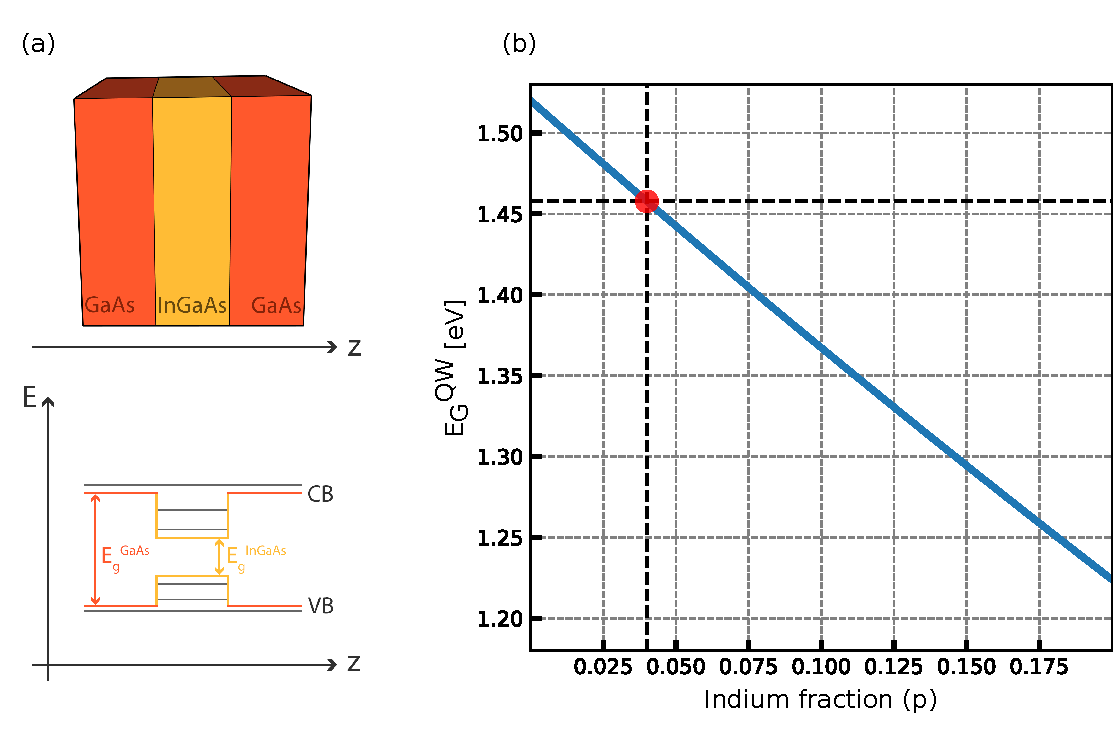
\includegraphics[width=0.8\linewidth]{chap_theory/fig/InGaAs.pdf}
    \caption{\textbf{Schematic representation of a quantum well heterostructure.} a) Representation of a planar quantum well made of InGaAs placed in between two layers of GaAs. The confinement in the plane is ensured by the gap energy difference between the layers.
    b) Gap energy of the InGaAs quantum well as a function of the dopping fraction of Indium. The red dot represent the dopping in sample used in the experiment : $E_g^{InGaAs} = 1.46 eV < E_g^{GaAs} = 1.52 eV$.}
    \label{fig:sc_quantum_well}
\end{figure}

Assuming the same geometry than the above figure the electron-hole hamiltonian taking into account the potential barrier is written in first quantization as :

\begin{equation}
    \Ham = E_g^{QW} + \dfrac{\mathbf{p}^2_e}{2m_e} + \dfrac{\mathbf{p}^2_h}{2m_h} - \dfrac{e^2}{\epsilon_{sc}|r_e-r_h|}+V_e(z_e)+V_h(z_h)
\end{equation}
where z is the growth axis of the quantum well and $V_e(z_e)$ and $V_h(z_h)$ are the potential barriers felt by the electron and the hole respectively, $r_e$ and $r_h$  are the electron and hole spatial coordinates. 
The system is invariant under translation in the $xy$-plane the excitons in plane wavevector $k_{\parallel}$ can then take any value while the confinement in the $z$-direction quantize the corresponding component of the wavevector $k_z$. 
This problem is treated by writting the exciton wavefunction $\Psi(x,y,z)$ as a two components product :

\begin{equation}
    \Psi(x,y,z) = \psi(x,y,z)\phi(z).
    \label{eq:2D_exciton_wavefunction}
\end{equation}

The Schrodinger equation is then solved separately for $\psi(x,y)$ and $\phi(z)$. 
The confinemnt in $z$-direction is treated as a very basic quantum box problem. The electron and hole energies are then quantized as :

\begin{equation}
    E_n^{e,h} = \dfrac{(\pi^2 n^2\hbar^2}{2m_{e,h}L_z^2}
    \label{eq:QW_energy_levels}
\end{equation}

where $L_z$ is the width of the quantum well.

To determine the in-plane wavefunciton we follow the same procedure than for the exciton eigenproblem in the 3D case.
The exciton is again a correlated pair whose center of mass is delocalized as a plane wave with momentum $\mathbf{Q} = \hbar \kpar$. The correspondig energy is then  :

\begin{equation}
    E_X^{xy} = E_g^{QW} + \dfrac{\mathbf{\hbar k_{\parallel}}^2}{2m_X} - \dfrac{R_X^{QW}}{n^2}
\end{equation}
provided that we defined a new Rydberg constant $R_X^{QW}$ taking into account the confinement in the $z$-direction. Remarkably, due to confinement the Bohr radius $a_X^{QW}$
of the QW exciton is twice smaller than the bulk exciton Bohr radius. This is a direct consequence of the confinement that increases the electron-hole wavefunctions overlap and thus the binding energy of the exciton. The exciton total energy is then : 

\begin{equation}
    E_X(\kpar) = E_g^{QW} + E_n^{e} + E_n^{h} +  \dfrac{\mathbf{\hbar k_{\parallel}}^2}{2m_X} - \dfrac{R_X^{QW}}{n^2}
    \label{eq:2D_exciton_energy}
\end{equation}
The design of the sample used in the experiement is done such as the n=1 level is sufficiently far form the next level that we can restrict our description to 
the first 1s exciton state. In the following we will therefore drop the n index by setting it to one.

\bigskip


\noindent \textbf{Bosonic nature of excitons.} Since an exciton is made of two fermions its pseudo spin is an integer. However, when reaching regimes of high excitons densities
the fermionic nature of their microscopic constitutives can no longer be neglected. The composite nature of excitons can then be safely dropped provided that the exciton density per unit area 
is such as $n_X(a_X^{QW})^2 \ll 1$. This condition state that the average distance between excitons is much larger than the exciton Bohr radius. In this regime the excitons can be treated as bosons, namely : 


\begin{equation}
    [b_{\mathbf{k}}, b^{\dagger}_{\mathbf{k}}] = 1 - O(n_X(a_X^{QW})^2) \simeq 1
    \label{eq:exciton_bosonic_nature}
\end{equation}

\bigskip



\noindent \textbf{Optical selection rules in the planar quantum well.}In bulk semiconductors, a single exciton mode couples exclusively to a single photon mode. In quasi-two-dimensional systems, due to the breaking of translationnal invariance in the growth direction $z$ the momentum
conservation during a photon absorption or emission remains valid only for the in-plane component, the $z$-component being fixed by the quantum well width.
Accordingly, an exciton with wavevector $\mathbf{k}_X=(\kpar^X, k_z^X)$ will interact with a photon with the same in plane wavevector but with any value of $k_z^\gamma$. 
There is thus a density of states for radiative decay given by (see \cite{weisbuch_microcavities_1996}):

\begin{equation}
    \rho_{2D}(\kpar, \hbar \omega) \equiv \sum_{k_z}\delta(\hbar\omega - \dfrac{\hbar c}{n_{QW}} \sqrt{\kpar^2+ k_z^2})\propto \dfrac{\hbar\omega}{\sqrt(k_0^2-\kpar^2)}\mathbf{\Theta}(k_0-\kpar)
    \label{eq:2D_dos}
\end{equation}
where where $n_{QW}$ is the refractive index in the QW, $k_0 = n_{QW}\omega/c$ is the wavevector of the photon in the material and $\Theta$ is the Heaviside step function. 
Only states with $|\kpar|<k_0$ can couple to light giving rise again to two class excitons.
\begin{itemize}
    \item States with $|\kpar^X|<k_0$ that couple to light. These states have a finite radiative lifetime $1/\gamma_X$ given by the Fermi Golden rule. They lie on the left of the
    light cone in the $\kpar-\omega$ plane.
    \item States with $|\kpar^X|>k_0$ that do not decay radiatively. They lie on the right of the photon line in the the $\kpar-\omega$ plane.  They are analog to surface
    modes as they have a vanishing electric field far from the QW. These states join the previously described excitons that could not couple to light because of their spin configuration to form
    a wider class of "dark" excitons.
\end{itemize}
This stands in contrast to bulk semiconductors, where a single exciton mode couples exclusively to a single photon mode.
Nevertheless, if we also 
impose energy conservation between the exciton and the photon mode the maximum in-plane wavevector of radiative excitons gets modified and depend on the exciton energy.
To see this let us consider an inital state made of an exciton of overall energy $E_X(\kpar^X)$ and zero photon and a final state made of a single photon with energy $E_\gamma(\kpar^{\gamma})= \frac{\hbar c}{n_{QW}} \sqrt{(\kpar^\gamma)^2+ (k_z^\gamma)^2}$ and no exciton.
The energy conservation of this process reads :

\begin{subequations}
    \begin{align}
    E_X(\kpar^X)&= E_\gamma(\kpar{\gamma}) \\
    E_X^{QW} + \dfrac{(\hbar\kpar^X)^2}{2m_X}  &= \dfrac{\hbar c}{n_{QW}} \sqrt{(\kpar^\gamma)^2+ (k_z^\gamma)^2},
    \end{align}
    \label{eq:energy_conservation}
\end{subequations}
in which we set $E_X^{QW} = E_g^{QW}+ E_X^{1s}= E_g^{QW} + E_1^{e} + E_1^{h}-R_X^{QW}$. Injecting the in-plane momentum 
conservation and imposing ${k_z^\gamma}^2 \geq 0$ for the photon field to be propagative the above condition restricts the exciton that can couple to light through :

\begin{equation}
    |\kpar^X| \leq \dfrac{cm_X}{n_{QW}\hbar}\left(1+\sqrt{1-\dfrac{4n_{QW}E_X^{QW}}{m_Xc^2}} \right).
    \label{eq:k_max}
\end{equation}
Since $E_X^{QW}$ can be negleted with respect to the exciton mass energy $m_Xc^2$ the above condition taken at first order gives :

\begin{equation}
    |\kpar^X| \leq \dfrac{n_{QW}E_X^{QW}}{\hbar c}.
    \label{eq:kmax_approx}
\end{equation}


\noindent Excitons with higher wavevector are than forbidden to exchange energy with light. However, in our case we have $E_X^{QW} \simeq 1.485  /  meV$ and $n_{QW} \simeq 3.5$ leading to $|\kpar^X| \leqslant 30 / \mu m^{-1}$ which is way beyond
the values adressed in the experiment. Now that the exciton formation is well etablished let us have a look at the mechanisms that can lead them to interact.
 

\subsection{Exciton-exciton interaction}
\label{sub:exciton_exciton_interaction}

The scope of this section is to answer the question of what can lead two excitons in states $(i,j)$ to end up in states $(f,g)$. Obviously, direct
coulomb interactions between the excitons constitutive is an unambiguous valid answer. Nonetheless, an interaction giving the same result can also occur in the absence of any Coulomb interactions via pure carrier exchange.
Namely, excitons $i$ and $j$ can exchange either their electron or hole. The latter is a direct consequences of the Pauli exclusion principle stating that two fermions cannot occupy the same quantum state. 


\subsubsection{Coulomb interaction}

As explained in the previous section, holes and electrons undergo Coulomb interaction. As a consequence, the interaction
between two excitons $(e_1,h_1)$ and $(e_2,h_2)$ consist of $V_{e_1e_2}+V_{h_1h_2}+V_{e_1h_2}+V_{h_1e_2}$. However, if the exciton were made of $(e_1,h_2)$ and $(e_2,h_1)$ the cross term in the interaction potentail would be replaced
by $V_{e_1h_1}+V_{e_2h2}$. Because there are different possible ways to form excitons, the total interaction energy depends on the specific pairing choice.
This makes it impossible to define a single, clean exciton-exciton interaction potential that works in all cases.
Hence, treating them as pure bosons with a simple interaction potential fail because the effective exciton-exciton potential is not unique and depends on the microscopic way the excitons are formed.
Nevertheless, it is clear that, through Coulomb interaction, excitons can change states and thus interact in the most general sense. This being said, we will as experimentalist, focus on the most 
important scattering process that is actually coming from exchange carrier among excitons and that is a unique feature of composite particle.

\subsubsection{Fermionic exchange interaction}

Let us consider two excitons $X_1=\ket{\mathbf{k_e},\mathbf{k_h}}$ and $X_2=\ket{\mathbf{k_e}',\mathbf{k_h}'}$. If their wavefunction
start to overlap the two electrons for example might see their qunatum state becaming almost equal which is forbidden by the Pauli exclusion principle. To regularize this situation 
the exciton can exchange their carrier to form $X'_1=\ket{\mathbf{k_e}',\mathbf{k_h}}$ and $X'_2=\ket{\mathbf{k_e},\mathbf{k_h}'}$. This is might look counterintuitive since exchanging two particles in the same quantum state doesn't seem to solve the problem. However,
it's truly the exchange process itself put together with wavefunction symmetries that modify the quantum state configuration to avoid Pauli principle violation.
Take two indistinguishable particles, in state $\psi_a$ and $\psi_b$ in a 1D system  \cite{CCT_tome2}. Normalization consideration aside, the wavefunction of the system can be written in two ways : $\psi_{ab} =\psi_a(x_1)\psi_b(x_2) \pm \psi_a(x_1)\psi_b(x_2)$.
Depending on the plus or minus sign, the wavefunction is symmetric or antisymmetric under position exchange. The two different configurations imply different physics.
For instance the mean value of the particle interdistance is :

\begin{equation}
    \langle(x_1-x_2)^2\rangle = \langle x_1^2\rangle + \langle x_2^2\rangle \mp 2\langle x_1x_2\rangle ,
\end{equation}

provided the wavefunctions overlap $\langle x_1x_2\rangle\neq0$, the expected value is decreased for bosons and increased for fermions. Although, it seems to act 
as a force repelling or attracting particles, it is rather a geometrical constraint arising from the Pauli principle and the quantum nature of the particle at stake.
This is precisely what happend during carrier exchange and can, at the end, lead to scattering processes between excitons. Forgetting about this interaction ad try to fully bosonize excitons would then be a mistake \cite{ciuti_carrier_exchanges_1998}.
As an example, some features experimentally measured like exciton stark effect, precisely needs to put exchange carrier on the table to be understood \cite{exciton_stark_VonLehmen_86,exciton_stark_Mysyrowicz_86,joffre_m_subpicosecond_1987}.
Furthermore, in a 2D quantum well system this scatterings are dominant at larger scale while direct Coulomb interactions are dominant at scales smaller than the Bohr radius of
excitons. Therefore, by considering only radiative modes, i.e. dynamics occuring on scales much larger than the Bohr radius of
excitons $ka_X\ll 1$, Coulomb interactions can be neglected. Despite all the differences with true bosons above mentionned and the hot debates still going on about polaritons interactions \cite{Combescot_2007_exact_pol_pol_interactions,I_frerot_PRX_2023} this enable us, as experimentalist, to escape from ambiguity and write the main exciton-exciton potential that 
will be relevant in the experiment reported in this work. Written in momentum space this exciton-exciton potential $V_{XX}(\kvec)$ appear as four body contact interaction \cite{Rochat2000}. The corresponding hamiltonian follows as :


\begin{equation}
    \Ham_{XX} = \dfrac{1}{2}\sum_{\kvec, \kvec', \vec{q}} V_{XX}(\vec{q}) \hat{b}^\dagger_{\kvec+\vec{q}} \hat{b}^\dagger_{\kvec'-\vec{q}} \hat{b}_{\kvec} \hat{b}_{\kvec'}.
\label{exciton_interaction_ham}
\end{equation}

The potential $V_{XX}(\vec{q})$ is a function of the exchanged momentum $\vec{q}$. However, it can be approximated by a constant in the limit of low wavevectors since, being four order of magnitude heavier than microcavities photons, their varies only slightly with $\kvec$ in the range of the photon wavevector that excite them. Therefore $V_{XX}$ can be assumed constant. The numerical calculation gives $A \times V_{XX}\simeq$ 3 $\mu$eV$\cdot \mu$m$^{2}$ for our InGaAs system.
\begin{equation}
    V_{XX} = \dfrac{e^2 a_X^{QW}}{\epsilon A},
\end{equation}

with $A$ the quantization area equal to the  quantum well surface. The numerical calculation gives $A \times V_{XX}\simeq$ 3 $\mu$eV$\cdot \mu$m$^{2}$ in our GaAs-InGaAs system.

\bigskip

\textbf{Dark excitons creation through carrier exchange.}

As discussed in \autoref{sub:exciton_photon_interaction} electron-hole pairs with a total spin of $\pm1$ are coupled to $\sigma\pm$ photons, meaning that photon absorption leads to the creation of only bright exciton states $\pm1$. However, dark exciton states can also be present in the system, arising from fermion exchange processes.
Namely, fermion exchange between two bright excitons $(+1,1)$ made of $(\mp1/2)$ electrons and $(\pm3/2)$ holes leads to dark excitons $(+2,-2)$. Hence, eventhough photon absorption only create bright excitons, excitons not coupled to light are likely to be indirectly excited and participate to the overall interactions of the system.
This being said, we will in the following only tackle this problem from a phenomenological point of view and consider the exciton-exciton interaction as a unique potential $V_{XX}$ whereas dark excitons will be accounted for thorugh a reservoir.

  
\section{Excitons-polaritons}
So far we described separately microcavity photons and excitons both in bulk and 2D systems. Microcavity polaritons arise from the
strong coupling between these two components. Remarkably, the half light half matter nature of polaritons allows them to inherit the best of both worlds namely 
the low photon effective mass and the strong excitons non linear interactions. In this section we will describe the formation of polaritons 
by decribing how placing a 2D semiconducting quantum well in an optical microcavity to enhance the light-matter interactions. To start with let us 
have a look a again at the Fermi Golden rule giving the spontaneous emission rate from a level $\ket{i}$ to a level $\ket{f}$ in a continuum of states per unit time in the presence of a weak coupling $W$ :

\begin{equation}
    \Gamma_{i\rightarrow f} = \dfrac{2\pi}{\hbar} \bigg|\bra{f}W\ket{i}\bigg|^2 \rho(E_f)\delta(E_f-E_i)
    \label{eq:fermi_golden_rule_1st_order}
\end{equation}
where $\rho(E_f)$ is the density of states at energy $E_f$ and $\delta(E_f-E_i)$ ensures energy conservation. 
Say, we want to "force" an exciton to recombine in a given photonic state $(\hbar \omega_\gamma, \mathbf{k}_\gamma)$. In a 2D quantum well,
an exciton with in plane wavevector $\kpar^X$ is allowed to couple to a continuum of photon modes provided their wavevectors respect \autoref{eq:kmax_approx}. 
Solving this problem boils down to changing the density of state $\rho$ in order to suppress sponatenous emission in all unwanted modes.
As usually done in cavity quantum electrodynamics, this problem is tackled by embedding the quantum well in an high finesse optical microcavity as shown in \autoref{fig:polariton_cavity} (a). 
\begin{figure}[]
    \centering
    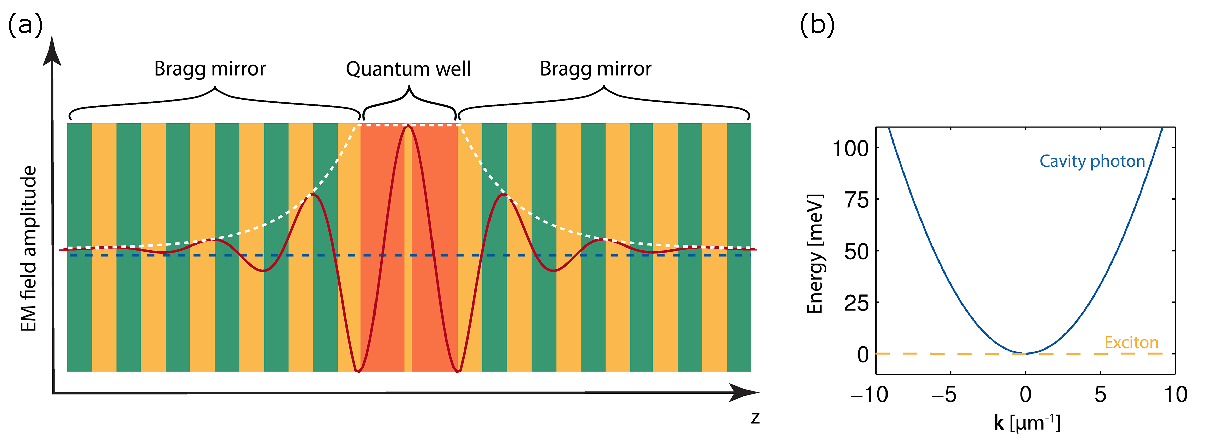
\includegraphics[width=0.8\linewidth]{chap_theory/fig/polariton_cavity.pdf}
    \caption{\textbf{Schematic representation of a quantum well embedded in an optical microcavity.} The quantum wells are placed at the antinode of the electric field of the cavity. The cavity is designed to have a single mode that matches the exciton energy.
    (b) Dispersions relation of the exciton (yellow) and photon (blue) modes in a typical microcavity. Since the exciton effective mass $m_X$ is $10^4$ times larger than the photon mass the exciton dispersion 
    looks flat with respect to the photon. The cavity has been designed so the $\kpar=0$ energies are matched.
    \label{fig:polariton_cavity}}
\end{figure}

The role of the latter is to create a set of resonant modes that will act as a "filter" for the exciton recombination. 
The quantization axis of the optical microcavity is chosen to be the same as the quantum well and the light-matter
interactions are optimized by placing the quantum well a the antinode of the electric field. The cavity length is chosen so that single photonic mode can be equal the excitonic energy.
This matching can be seen by looking simultaneously at the exciton and photon dispersion relation as a function of the in plane wavevector and check that they cross each other at a finite wavevector. For instance in the case of \autoref{fig:polariton_cavity} (b) the cavity has been designed so that the exciton and photon energies are equal at $\kpar=0$.
Several quantum well can then be stacked in the cavity to enhance the interactions provided that they are once again located at antinodes of the photonic field.
In the experiment we use a $3\lambda/2$ made of two planar DBR in which are placed three $InGaAs/GaAs$ quantum wells. An extended description of the fabrication procedure to built such a sample can be
found in \cite{maitre_thesis}. However, the main features mentionned so far can be summarized in a few points :

\begin{itemize}
    \item The cavity is made by embedding semiconducting quantum wells in between two distributed bragg reflectors forming a high finesse optical microcavity.
    \item The length of the cavity and of the wells are chosen so a single longitudinal mode of the electric field is resonant only with the 1s state of the exciton.
    \item The exciton are confined in the $xy$-plane in each quantum well and the exciton density can be tuned by changing the number of quantum wells.
    \item Momentum conservation still holds in the plane of the cavity. Namely, an incoming photon with wavevector $\kpar$ will create an exciton with the same in-plane wavevector. 
\end{itemize}
It appears then that the relevant motion of the interacting particles at stake lies in the $xy$-plane since the wavevectors in 
the  $z$-direction are fixed by the cavity parameters. Consequently, for sake of clarity, we will only refer to the in-plane wavevector in the following
by dropping the $\parallel$ label and just write $\kvec$.

\noindent Now that that some efforts were put in enhancing exciton-photon interactions let us see the different coupling regimes that we can be reached in such samples. 



\bigskip
\noindent \textbf{Coupling regimes.} At first approximation the problem can be thought as two bath of particles 
exchanging quanta at a rate $\OmR$. Depending on the efficiency of this exchage compared to
the damping rate of each bath $\gamma_X$ and $\gamma_{\gamma}$ one has to revisit the way to describe the system. Indeed, when 
$\OmR \ll \gamma_X, \gamma_{\gamma}$ the system is said to be in the weak coupling regime. It can be understood in terms of lifetimes : both excitons and photons lifetimes are too short compared to the 
characteristic time of the exchange $1/\OmR$. The energy leaks out of the system before it can change from one state to the other. The exciton-photon interaction is in this case irreversible.
If $\OmR \gg \gamma_X, \gamma_{\gamma}$ the system is said to be in the strong coupling regime. In a given photonic (or excitonic) lifetime $1/\gamma_{cav}$,
the answer to the question "where is the energy ?" is no longer clear. Indeed the energy have had enough time to coherently go back and forth between exciton and photon states plenty of times. Translating
this in quantum mechanics language simply means that the system is in a superposition of exciton and photon states. Polariton then rise in this regime as
as supersposition of microcavity photons and excitons exchanging energy at the so called Rabi frequency $\OmR$. 

\bigskip

\textbf{Linear Hamiltonian.} Let us write formally the coupling between excitons and photons described above. First we tackle
the weak optical excitation scheme in which non linear interactions among excitons can be neglected. The corresponding linear Hamiltonian 
is given by : 

\begin{equation}
    \Ham_{lin} = \sum_{\mathbf{k}}\left[E_X(\mathbf{k})b^{\dagger}_{\mathbf{k}}b_{\mathbf{k}} + E_{\gamma}(\mathbf{k})a^{\dagger}_{\mathbf{k}}a_{\mathbf{k}} + \dfrac{\hbar\OmR}{2}a^{\dagger}_{\mathbf{k}}b_{\mathbf{k}} + a_{\mathbf{k}}b^{\dagger}_{\mathbf{k}}\right]
    \label{eq:linear_hamiltonian}
\end{equation}
where $b^{\dagger}_{\mathbf{k}}$ and $a^{\dagger}_{\mathbf{k}}$ are the creation operators of the exciton and photon modes respectively. The first two terms account for the energies of the excitons and the photons while 
the terms $b^{\dagger}_{\mathbf{k}}a_{\mathbf{k}}$ and $a^{\dagger}_{\mathbf{k}}b_{\mathbf{k}}$ account for the linear exciton-photon coupling yielding an interaction energy $\hbar\OmR$. 
Obviously this hamiltionian is not diagonal in the excitons-photons operators basis.
Excitons-polaritons then arise as the two eigenstates of $\Ham_{lin}$ : the upper and the lower polaritons whose creation and annihilation operators are  $(\ukdag, \uk)$ and $(\pkdag, \pk)$ respectively.
These operators can be found by an unitary transormation on the exciton-photon basis that was extensively used by Hopfield \cite{hopfield_theory_1958}  :


\begin{equation}
    \label{eq:unitary_transformation}
    \begin{bmatrix}
    \pk \\
    \uk
    \end{bmatrix} 
    = 
    \begin{bmatrix}
    C_\kvec & X_\kvec \\
    X_\kvec & -C_\kvec
    \end{bmatrix}
    \begin{bmatrix}
    \ak \\
    \bk
    \end{bmatrix},
\end{equation}

where $C_\kvec$ and $X_\kvec$ are the Hopfield coefficients for photons and excitons respectively. The unitarity of the transformation
is reflected by the relation $C_\kvec^2 + X_\kvec^2 = 1$. As a consequence, they can be interpeted as the fractions of excitons and photons in both modes.
More precisely they depend on the excitons/photons energies and the Rabi frequency as : 

\begin{subequations}
    \begin{align}
    C_\kvec^2 &= \dfrac{\sqrt{\DeltaEX^2 + \hbar^2\OmR^2}- \DeltaEX}{2\sqrt{\DeltaEX^2 + \hbar^2\OmR^2}}, \\[5mm]
    X_\kvec^2 &=  \dfrac{\sqrt{\DeltaEX^2 + \hbar^2\OmR^2}+ \DeltaEX}{2\sqrt{\DeltaEX^2 + \hbar^2\OmR^2}}.
    \end{align}
    \label{eq:hopfield_coefficients}
\end{subequations}
where $\DeltaEX(\kvec) = E_{\gamma}(\kvec)-E_X(\kvec)$ is the detuning between the exciton and the photon energies at $\kvec$. 
In this basis the linear hamiltonian can be written in its diagonal form.



\begin{equation}
    \Ham_{lin} = \sum_{\mathbf{k}}\left[E_{LP}(\mathbf{k})\ukdag\uk + E_{UP}(\mathbf{k})\pkdag\pk\right]
    \label{eq:linear_hamiltonian_diagonal}
\end{equation}
where the eigenvalues $E_{LP}(\mathbf{k})$ and $E_{UP}(\mathbf{k})$ are the lower and upper polariton dispersion relation. Their analytical expressions 
are given by :

\begin{equation}
    \begin{align}
    E_{LP}(\mathbf{k}) &= \dfrac{E_X(\mathbf{k})+E_{\gamma}(\mathbf{k})}{2} - \dfrac{\sqrt{\DeltaEX^2 + \hbar^2\OmR^2}}{2}, \\[5mm]
    E_{UP}(\mathbf{k}) &= \dfrac{E_X(\mathbf{k})+E_{\gamma}(\mathbf{k})}{2} + \dfrac{\sqrt{\DeltaEX^2 + \hbar^2\OmR^2}}{2}.
    \end{align}
    \label{eq:polariton_dispersion}
\end{equation}

\textbf{Tuning the exciton-photon fraction.} As it can be seen the weight of photon and exciton in a given polaritonic state can be then tuned by changing the exciton-photon detuning 
$\DeltaEX$. Particurlarly, when $\DeltaEX = 0$ we have $C_\kvec^2= X_\kvec^2 = \frac{1}{2}$ meaning that the exciton and the photon are equally mixed in the polariton states. In practice, there are two ways to change the exciton-photon detuning. The first tuning knob, which is the most obvious, is the wavevector $\kvec$. Since the exciton
dispersion is flat with respect to the photon it boils down to move on the photon dispersion curve. Still, exciting a polariton state with a given set of Hopfield coefficients will fix the wavevector and, in some case might not be even possible. 
For instance if the photonic dispersion is above the exciton energy at all wavevector as in   \autoref{fig:wedge_and_hopfields} $\mathrm{b_1)}$, it is impossible to reach the purely hybrid configuration $\DeltaEX = 0 $. Creating an arbitrary polaritonic state thus require a second knob to tune $\DeltaEX$. It is generally done by introducing a small wedge between the two DBR that will change the photon resonance condition as shown in \autoref{fig:wedge_and_hopfields} a) : a change in the cavity length $L$ will shift vertically the photon disperions.
 Luckyly, this comes for free with the usual Molecular Beam Epitaxy method used to grow the sample.
The principle is to heat the target material to its sublimation temperature to produce a molecular beam that is then deposited on a substrate to form thin atomic layers that stack on top of each other.
In practice, the substrate is located on a spinning disk to avoid the molecule to clusterise. If the spinning disk is stopped, molecules will accumulate in the center of the beam and form a "hill".
By taking advantages of this features it is possible to change progressively the thickness of the layer and thus the cavity resonance condition. A given sample
has in fact a wide range of exciton-photon detuning that can be adressed in the lab by changing the working point on the cavity. 

\begin{figure}[]
    \centering
    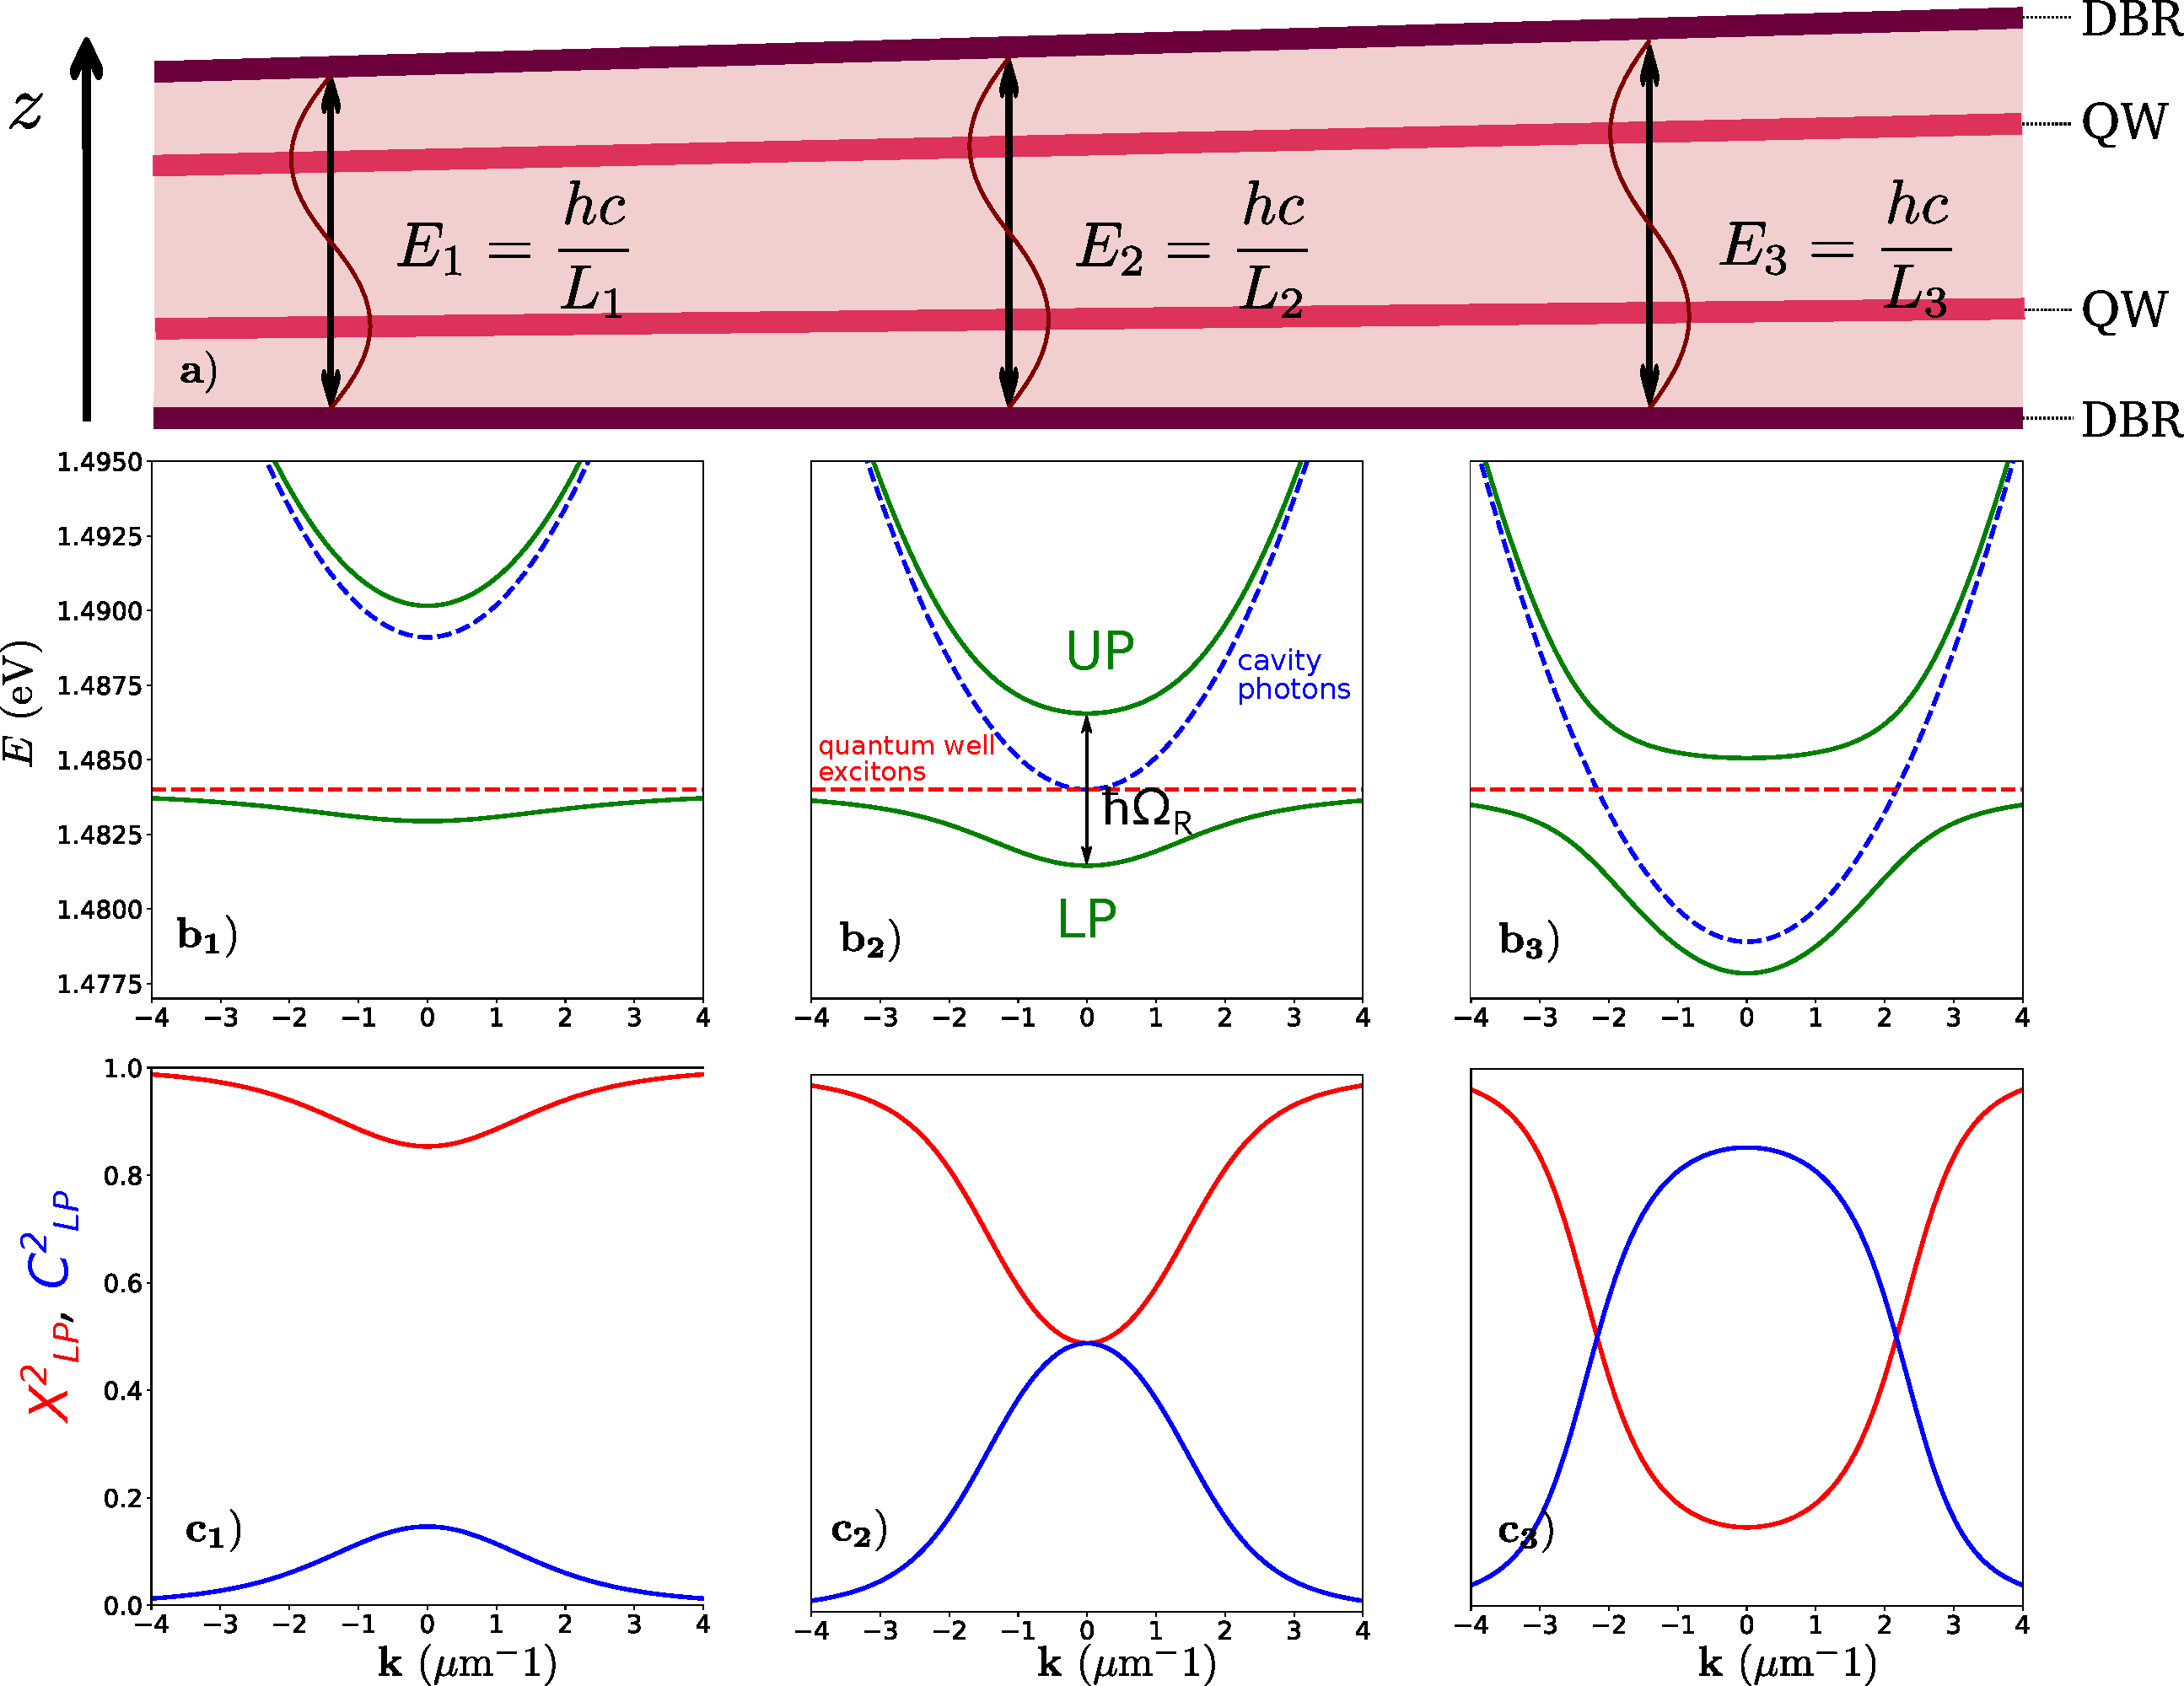
\includegraphics[width=1\linewidth]{chap_theory/fig/wedge_and_hopfields.pdf}
    \caption{\textbf{Scheme of an optical microcavity with a wedge, polaritons dispersion relations and Hopfield coefficients.} \textbf{a)} Side view of a
    double quantum well semiconducting microcavity. From left to right the photon resonant energy decreases as the length of the cavity increases. The exciton energy remains constant since it is fixed by the width of the quantum well.
    We take as example three point in the sample $i=1,2,3$ with increasing cavity length. At each point the wavy lines represent the optical standing wave stemming from the resonance conditions $\lambda_i = L_i$
    The corresponding energies $E_i$ illustrate the three different regimes namely : $\DeltaEX^{(1)}(\kvec=0) >0 , \DeltaEX^{(2)}(\kvec=0)=0 , \DeltaEX^{(3)}(\kvec=0) <0 $. Each $E_i$ corresponds to the subplots
    $\mathrm{b_i)}$ and $\mathrm{c_i)}$. $\mathbf{b_1), b_2), b_3)}$ Dispersion relations of the lower (LP) and upper polaritons (UP) in a typical microcavity for each value of $\DeltaEX^{(i)}$. The exciton energy is the yellow dashed line while the photon energy is the blue dashed line. Depending on the location
    on the sample $i=1,2,3$ the photon dispersion curve gets shifted vertically yielding different values of the Hopfield coefficient. $\mathbf{c_1), c_2), c_3)}$ Corresponding Hopfield coefficients as a function of the in-plane wavevector for the three different regimes. Adapted from \cite{claude_phd}.
    \label{fig:wedge_and_hopfields}}
\end{figure}

In general, when the exciton-photon detuning is too positive the UP branch recovers the excitons curve while the LP branch recovers the photons curve. Conversely,
when the exciton-photon detuning is negative the UP branch recovers the photons curve while the LP branch recovers the excitons curve. This is not very suprising
since a great detuning means that the exciton and the photon are far from each other making the coupling less efficient.  At the zero detuning point 
$\DeltaEX=0$ the coupling is maximum and the splitting between the lower and upper polariton branch is equal to the Rabi energy frequency $\hbar\OmR$. Besides, the anticrossing
between the two branches is a direct consequence of the strong coupling regime and can be find even in classical systems like coupled pendulums. 

The suitable range of detuning for which the polariton concept is still relevant and that we can adress in the experiment is shown in \autoref{fig:anticrossing}
\bigskip

\textbf{Relaxation.} The strong coupling condition $\OmR \gg \gamma_X, \gamma_{cav}$ can also be seen by directly taking into account
the finite lifetime of excitons and photons, introducing imaginary energies $E_{\gamma}-i \gamma_{cav}$ and $E_X-i\gamma_X$ as in \cite{cohen-tannoudji_photons_2004}.
Doing so, the polariton dispersions relation become :

\begin{align}
    \begin{split}
        E_{UP, LP}(\kvec) ={}& \dfrac{\Eph(\kvec) + \Eex(\kvec)}{2} - i \hbar \dfrac{\gamma_{cav} + \gamma_X}{2}
        \\& \pm \dfrac{1}{2} \sqrt{\left[ \hbar \OmR \right]^2 + \left[ \DeltaEX - i \hbar (\gamma_{cav} -  \gamma_X )\right]^2}.
    \end{split}
    \label{polariton_disp_loss}
    \end{align}
At zero detuning we obtain :

\begin{equation}
        E_{UP, LP}(\kvec) =\Eex(\kvec) - i \hbar \dfrac{\gamma_{cav} + \gamma_X}{2} \pm \dfrac{1}{2} \sqrt{(\hbar \OmR) ^2 +  (\hbar\gamma_{cav} - \hbar \gamma_X )^2}.
    \label{polariton_disp_loss_zero_det}
\end{equation}
The existence of two distinct energies for the two polaritons modes thus depends on the relative values of $\OmR$ and $|\gamma_{cav} - \gamma_X|$.
 If the coupling constant $\OmR$ is smaller than the difference between the relaxation constants, the two eigenenergies share the same real part, and the degeneracy between the exciton and the cavity mode remains unbroken.
Being a supersposition of excitons and photons the polaritons also have a relaxation rate that can then be inferred from the imaginary part of their energy :

\begin{subequations}
    \begin{align}
    \gamma_{UP}(\kvec)&= X_\kvec^2\gamma_{cav} + C_\kvec^2\gamma_X, \\[5mm]
    \gamma_{LP}(\kvec)&= X_\kvec^2\gamma_X + C_\kvec^2\gamma_{cav}.
    \end{align}
    \label{eq:polariton_relaxation}
\end{subequations}
Once again, the hopfield coefficient have a strong impact on the polariton relaxation rate. In the range of detuning
available in our sample we measure relaxation rates of the order of  $\SI{70}{\micro\electronvolt}$ which correspond to a lifetime  
$\tau \sim \SI{10}{\pico\second}$. This value is beyond the time response of a wide class of instruments and require generally both pulsed lasers and ultrafast
detection devices to be resolved as in \cite{Utsunomiya_fluidlightexp_2008}. The present work is not dedicated to time resolved experiments as we rather use a continuous wave laser to constantly compensate for the losses and reach a steady state from which we extract observable quantities. This system is then highly out of
equilibrium. Although this feature seems limiting at first sight it can actually turn into an asset whenever one wants to study dynamical instabilities. Indeed, in conservative systems, 
instabilities are difficult to study precisely because they tend to make the system unstable. In the case of polaritons, the losses can reduce 
their effect while keeping their signature visible in the steady state of the system \cite{claude_high-resolution_2022}.

\bigskip


\textbf{Effective mass.} By analogy with was done for the photons in \autoref{sec:photon} it is possible to affiliate an effective mass to the polaritons
by taking the second derivative at the bottom of the polariton dispersion relation, namely :

\begin{subequations}
    \begin{align}
    \dfrac{1}{m_{UP}} &= \dfrac{X_0^2}{m_X}+\dfrac{C_0^2}{m_{\gamma}}, \\
    \dfrac{1}{m_{LP}} &= \dfrac{X_0^2}{m_{\gamma}}+\dfrac{C_0^2}{m_X}.
    \end{align}
\end{subequations}
Reminding that $C_0^2 + X_0^2 = 1$ and that $\frac{m_\gamma}{m_X}\ll 1$. It can be cast in the following form :

\begin{subequations}
    \begin{align}
    m_{UP} &\approx\dfrac{m_\gamma}{X_0^2} \\
    m_{LP} &\approx\dfrac{m_X}{C_0^2}
    \end{align}
    \label{eq:polariton_effective_mass}
\end{subequations}
It can be seen that polaritons inherit the low effective mass of the photons making their transport easier than for excitons.
This is particularly interesting for the realisation of polaritonic circuits in the framework of quantum information processing \cite{liew_optical_circuit_2008}.
The excitonic part of the polariton also bring its own features to the table. In particular, the strong exciton-exciton non linear interactions that
will turn light into a fluid of interacting particles. This is the subject of the next section.
\begin{figure}[h]
    \centering
    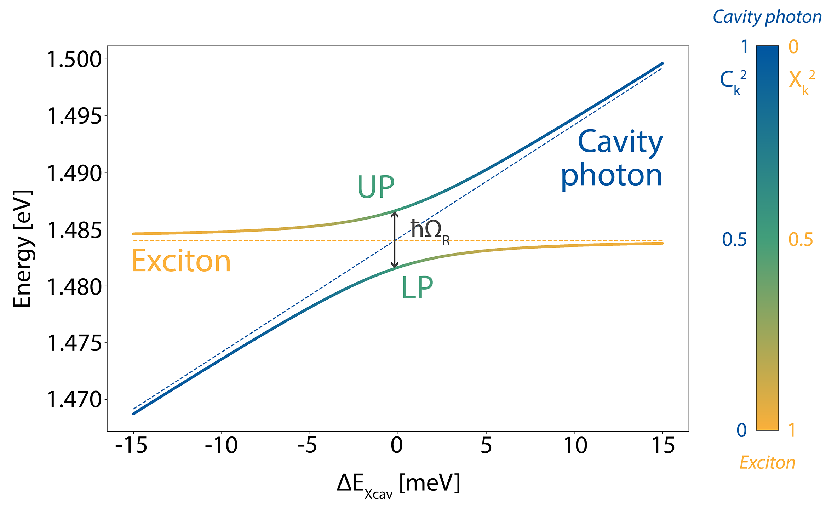
\includegraphics[width=0.75\linewidth]{chap_theory/fig/anticrossing.pdf}
    \caption{\textbf{Anticrossing in the strong coupling regime.} Energies of the upper (UP) and lower (LP) polariton branches at $\kvec = 0 \mathrm{\mu m^{-1}}$, with respect to the exciton-photon detuning at zero wavevector $\DeltaEX(\kvec=0)$ and the color-coded squared modulus of the Hopfield coefficient $X^2$ (exciton) and $C^2$ (photon). The yellow and blue dashed lines are respectively the bare exciton and photon energies. 
    At $\DeltaEX$ = 0 meV, the coupling is the better yielding an energy splitting equal to the Rabi energy $\hbar \OmR$. Adapted from \cite{maitre_thesis}}. 
    \label{fig:anticrossing}
\end{figure}

\subsection{Polariton interactions}
\label{sub:polariton_interactions}

It is now clear that shinning a strong laser with the right frequency on a semiconducting microcavity will create plenty of polaritons. Since the have an excitonic part,
they may undergo many body effects that were not taken into account in the linear hamiltonian model derived earlier. More precisely, polaritons experience 
all the exciton-exciton interactions described in \autoref{sub:exciton_exciton_interaction} as well as additional features coming from their coupling with light.
Remarkably, in high density regime the Pauli principle has to apply again on the electrons and the holes leading to carrier exchanges. In the absence of light
these fermionic exchanges are actually the dominant scatterings processes while the direct Coulomb scattering is negligible as was explained in \autoref{sub:exciton_exciton_interaction}.
We remind the expression of the resulting exchange hamiltonian :

\begin{equation}
    \Ham_{XX} = \dfrac{1}{2}\sum_{\mathbf{k}, \mathbf{k}', \mathbf{q}}V_{XX}\left[p^{\dagger}_{\mathbf{k+q}}p^{\dagger}_{\mathbf{k'-q}}p_{\mathbf{k}}p_{\mathbf{k'}}\right]
    \label{eq:direct_pol_interaction}
\end{equation}

When the excitons are strongly coupled to cavity photon these carrier exchanges give rise to an additional saturation potential describing what was called a "photon-assisted exchange scattering" in the proposal of \cite{Combescot_2007_exact_pol_pol_interactions}.:


\begin{equation}
    \Ham_{sat} = \dfrac{1}{2} \sum_{\kvec, \kvec', \mathbf{q}} V_{sat} \left[ a^\dagger_{\kvec+ \mathbf{q}} b^\dagger_{\kvec'- \mathbf{q}} b_{\kvec} b_{\kvec'} + h.c. \right],
\end{equation}
where $V_{sat}$ is the saturation potential that can be computed by applying the Usui transformation on the quantum wells \cite{usui_sat_potential_1960}.

\begin{equation}
    V_{sat}=\dfrac{\hbar\OmR}{An_{sat}},
\end{equation}

in which $n_{sat}$ is the saturatiion density computed from the 2D exciton bohr radius as $n_{sat}=1/a_X^{QW}$ and A the macroscopic quantization area.
\textcolor{red}{This scattering can be understood from a microscopic point of view. Consider two excitons, $i_1$ and $i_2$, in a first step they exchange their carrier without any Coulomb process giving
two other excitons $i_1'$ and $i_2'$. In a second step, one of the exciton, let us say $i_1'$ find itslef in the same state than a neighbouring exciton. Because of the Pauli principle it can not stay in this state. Luckyly it is couple 
to cavity photon which enable it to get out of this irregular situation by emitting a photon.}
To end up with a description of interactions in the polariton basis we invert the unitary transformation in \autoref{eq:unitary_transformation} : 

\begin{subequations}
    \begin{align}
        \bk &=X_k \pk -C_k\uk, \\
        \ak &=C_k \pk +X_k\uk,
    \end{align}
\end{subequations}
and inject these expressions into $\Ham_{XX}$ and $\Ham_{sat}$. We end up with a single polariton-polariton potential that is a combination of hopfield coefficients, $V_{sat}$ and $V_{XX}$.
For the lower polaritons, which are the one we excite in the experiment and to which we will restrict in the following we obtain an effective polariton-polariton potential $V_{pp}$ as :

\begin{equation}
    V_{pp}= |X_\kvec|^4V_{XX}+2|X_\kvec|^2X_\kvec C_\kvec V_{sat}.-
\end{equation}
Once again it depends on the exciton-photon fraction through the Hopfield coefficients, and, in the purely hybrid situation $\DeltaEX$=0, yields $A \times V_{pp}= \SI{1}{\micro\electronvolt \per\square\micro\meter}$ in our sample.

\bigskip

\textbf{Non linear LP hamiltonian.} Finally, taking into account the polariton-polariton interactions abovementionned the linear hamiltonian for Lower Polaritons can be completed as follows :

\begin{equation}
    \Ham_{LP} = \sum_{\mathbf{k}}\hbar\omega_{LP}(\mathbf{k})\pkdag\pk + \dfrac{1}{2}\sum_{\kvec,\kvec',\mathbf{q}}V_{pp}\left[p_{\kvec+ \mathbf{q}}^{\dagger}p_{\kvec'- \mathbf{q}}^{\dagger}p_{\kvec}p_{\kvec'}\right].
    \label{eq:pol_non_linear_hamiltonian}
\end{equation}

\textbf{Energy renormalization.} As it can already be seen in the LP non linear hamiltonian, the bare polartion energies are no longer eigenvalues of the system in the presence of interactions.
To give a simple picture of this feature let us restrict the description to two polariton modes $p_{\mathbf{k_1}}$ and $p_{\mathbf{k_2}}$.
If the system is prepapred in such a way as to populate one of the two modes, $\mathbf{k_2}$, this macroscopic reservoir of polaritons acts as an external potential for the polaritons in the poorly populated mode $\mathbf{k_1}$. Consequently, the energy of the polaritons in mode $\mathbf{k_1}$ increases by an amount corresponding to the potential created by the polaritons in mode $\mathbf{k_2}$. 
This is a phenomenon of energy renormalization.

To be more quantitative, we can write the Hamiltonian of the system while restricting it to these two modes. In this case, $\Ham_{int}$ is the sum of $p^\dagger_\mathbf{k_1}p^\dagger_\mathbf{k_2}p_\mathbf{k_1}p_\mathbf{k_2}$ and $p^\dagger_\mathbf{k_2}p^\dagger_\mathbf{k_1}p_\mathbf{k_2}p_\mathbf{k_1}$. Since $p_\mathbf{k_2}$ and $p_\mathbf{k_1}$ are eigenstates of the system, they commute, meaning that the two previous term account for the same scattering.
The time evolution of $p_{\mathbf{k_1}}$ can then be described by the Heisenberg equation : 

\begin{equation}
    i\hbar \dfrac{d}{dt}p_\mathbf{k_1} = [p_\mathbf{k_1}, \Ham_{LP}] = [p_\mathbf{k_1},\Ham_{lin}] + [p_\mathbf{k_1},\Ham_{int}].
\end{equation}

the interacting term being :

\begin{equation}
    [p_\mathbf{k_1},\Ham_{int}]=\dfrac{V_{pp}}{2}p^\dagger_\mathbf{k_2}p^\dagger_\mathbf{k_2}p_\mathbf{k_1}= \dfrac{\hbar g_{LP}}{A}\hat{N}_{2}p_\mathbf{k_1}.
\end{equation}
$\hat{N}_{2}$ is the number operator in mode $\mathbf{k_2}$ and $\hbar g_{LP} = V_{pp}A/2$  is the polariton-polariton interaction constant. Since, the mode 
$\mathbf{k_2}$ is macroscopically populated, we can replace $\hat{N}_{2}$ by its expectation value $\langle \hat{N}_{2} \rangle$, which exhibit the polariton density in mode $\mathbf{k_2}$, $n_{2}=\langle \hat{N}_{2} \rangle/A$.
As a result, the master equation for the $\kvec_1$ gets renormalized by interactions with the $\kvec_2$ mode as :

\begin{equation}
    i\hbar \dfrac{d}{dt}p_\mathbf{k_1} = \left[\hbar\omega_{LP}(\mathbf{k_1}) + \hbar g_{LP}n_{2}\right]p_\mathbf{k_1}.
    \label{eq:renormalized_energy}
\end{equation}
where $\omega_{LP}(\mathbf{k_1})=E_{LP}(\kvec_1)$ is the bare energy of the polariton with wavevector $\kvec_1$. Although this is a simplified model with only two modes, the equation demonstrates how interactions between polaritons can lead to the renormalization of their energies. More generally, this phenomenon takes place between all modes in the system, including self-interactions of individual modes.
 The latter closely resembles the optical Kerr effect, where a field modifies the refractive index of the medium through which it propagates.

\section{Polariton dynamics}

\indent 

To summarize, microcavity exciton-polaritons are hybrid light-matter quasiparticles that combine characteristics of both components. 
Their photonic part endows them with an exceptionally low effective mass and allows us to manipulate them using light. 
Conversely, their excitonic part provides them with the exotic properties associated with electrons in semiconductors. 
Although the resulting interactions are varied and stem from different origins, they can, to a first approximation, be described by a single four-body contact potential, $V_{pp}$.

In this framework, polaritons can be viewed as weakly interacting bosons, distinguished by their inherent losses, making their behavior an out-of-equilibrium problem. 
In the following, we will explore their dynamics when one or a few modes are macroscopically populated, revealing remarkable phenomena typically associated with true many-body bosonic systems, such as superfluidity and Bose-Einstein condensation (BEC).
 However, whenever necessary, we will return to their composite fermionic nature to account for unique features that may not be captured by the mean field approximation.
 
\subsection{Mean field approximation}

\indent

In order to describe the dynamics of the polariton fluid of light, it is convenient to use the mean field approximation as it is usually done for quantum fluids \cite{pitaevskij_bose-einstein_2016}. This assumption is valid when the number of particles is large $N \sim N+1$ and when the major part of them occupy the same quantum state.
Obviously, the latter can happen only in bosonic systems since fermions obey the Pauli exclusion principle. In atomic systems, the macroscopic occupation occurs in the ground state of the system, and, provided that the temperature is low enough, happens spontaneously due to bosonic stimulation. In the case of polaritons, the situation is dramatically different since the system is out of equilibrium and the particles have to be continuously pumped to compensate for the losses.
The mean field of the system is then rather a steady state than a ground state at equilibrium. This being said, it is still possible to define a macroscopic occupation of a given mode in the system.
Whenever this happens, the theoretical procedure boils down to replacing the field operator $\hat{\psi}(\mathbf{r},t)= \sum_{k}\varphi_\kvec \hat{p}_\kvec$ that annihilates a particle at ($\mathbf{r}$,t), by its expectation value $\langle \hat{\psi}(\mathbf{r},t)\rangle$. This idea is supported by
by the fact that, in such situations, adding or removing a particle from the system does not change its state. The system is then described by a single classical wavefunction whose square modulus gives the density of particles in the system $|\psi(\mathbf{r},t)|^2= n(\mathbf{r},t)$ and with a well defined phase 
accounting for long range coherence. However, it doesn't mean that the system has became fully classical. Indeed, its quantum nature is hidden in the fluctuations around the mean field and often manifest itself through collective behavior. Accounting for these fluctuations is done 
by adding a small perturbation to the mean field : 

\begin{equation}
    \label{eq:mean_field_and_fluctuation}
    \hat{\psi}(\mathbf{r},t) = \langle \psi(\mathbf{r},t) \rangle + \delta \psi(\mathbf{r},t).
\end{equation}

For now let us focus on the description of the mean field dynamics and justify more quantitavely the relevance of describing a polariton fluid with a single wavefunction.

\bigskip

\textbf{One wavefunction to rule them all.} A pioneering result in the early stages of quantum mechanics is the so called wave-particle duality proposed by Louis de Broglie \cite{deBroglie1925} in 1924.
It states that particles can exhibit both wave and particle properties. 
More precisely, to any particle with momentum $\mathbf{p}$ can be associated a wavelength $\lambda=h/|\mathbf{p}|$. This wavelength is the characteristic of the wave associated with the particle and is called the de Broglie wavelength. 
As a result if two particle are separated by a distance smaller than their de Broglie wavelength their corresponding wavefunction will sum and possibly give rise to wave like effect as interferences.
This idea was later confirmed by the famous double slit experiment in which electrons were sent through a double slit and displayed an interference pattern.

If one apply this idea to a great number of particle in the same quantum states whose inter-particle distance is smaller than $\lambda$ it is no longer possible to distinguish them and they can be described by a single wavefunction.
At thermal equilibrium the momentum of a particle follows a Maxwell Boltzmann distribution and the de Broglie wavelength is of the order of the thermal de Broglie wavelength :
\begin{equation}
    \lambda_T = \dfrac{h}{\sqrt{2\pi m k_B T}},
    \label{eq:thermal_deBroglie}
\end{equation}
where $T$ is the temperature $m$ the particle mass and $k_B$ the Boltzmann constant. From this simple formula, one can see why reaching long range coherence in a system often require trapping and cooling procedures. In the case of polaritons,
a typical polariton-polariton inter-distance is about $\SI{0,1}{\micro\meter}$ while the small polaritons effective mass and the cryogenic temperature ($\sim 4K$) yields a thermal de Broglie wavelength of the order of $\SI{1}{\micro\meter}$ which validates the mean field approximation.
Now that we have a single order parameter to describe the system, let us see how it evolves in time.

\bigskip

\subsection{Driven dissipative Gross-Pitaevskii Equation.}
In the context of Bose gas this problem was first tackled by Gross \cite{Gross1961} and Pitaevskii \cite{pitaevskii1961} to describe
the structure of quantized vortices in liquid Helium. The resulting equation is known as the \textit{Gross-Pitaevskii equation} or non-linear Schrödinger equation :

\begin{equation}
     i\hbar \dfrac{\partial}{\partial t} \psi(\rvec, t) = \left( -\dfrac{\hbar^2}{2 m}\nabla_\rvec^2 + V_{ext}(\rvec) + \hbar g \abs{\psi(\rvec, t)}^2 \right) \psi(\rvec, t),
\label{GPE}
\end{equation}
where $g$ is the interaction constant, $\nabla_\rvec$ the kinetic energy and $V_{ext}(\rvec)$ is the external potential experienced by the particles. To extend this equation to the out of equilibrium polariton case, a first formulation in 
terms of exciton and photon reveals to be enlightening to identify the various corrections that must be considered.
Losses are incorportated through the relaxation rates $\gamma_X$ and $\gamma_{cav}$ while the continuous injection of photons in the system is accounted for by a pumping term $F_p(\rvec,t)$ in the photon field master equation.
Considering these terms we end up with a set of coupled equation for the exciton and photon fields $\psi_X(\rvec,t)$, $\psi_{\gamma}(\rvec,t)$ :

\begin{equation}
    i\hbar \dfrac{d}{dt}
    \begin{bmatrix}
    \psi_{\gamma}(\rvec, t) \\
    \psi_{X}(\rvec, t)
    \end{bmatrix} 
    = 
    \begin{bmatrix}
    \hbar F_p(\rvec, t) \\
    0
    \end{bmatrix} +
\label{Schrödinger_uncoupled}
\end{equation}
\begin{align*}
    \left( \Ham_{lin}(\rvec) + 
    \begin{bmatrix}
    V_\gamma(\rvec) - i\hbar \dfrac{\gamma_{cav}}{2} & 0\\
    0 & V_X(\rvec) - i\hbar \dfrac{\gamma_{X}}{2} + \hbar g_{XX} n_{X}(\rvec, t)
    \end{bmatrix}
    \right)
    \begin{bmatrix}
    \psi_{\gamma}(\rvec, t) \\
    \psi_{X}(\rvec, t)
    \end{bmatrix},
\end{align*}    
where $V_\gamma(\rvec)$ and $V_X(\rvec)$ are the mean external potentials felt by photons and excitons respectively, $g_{XX} = A V_{XX}/2\hbar$ is the exciton interaction strength and $n_X = \abs{\psi_{X}}^2$ is the exciton density.  Additionally, $\Ham_{lin}(\rvec)$ corresponds to the linear Hamiltonian from \autoref{eq:linear_hamiltonian_diagonal}, expressed in real space by substituting $\kvec$ with $i \nabla_\rvec$.

\begin{equation}
    \Ham_{lin}(\rvec)
    = 
    \begin{bmatrix}
    \hbar \omega_X & \hbar \OmR / 2 \\
    \hbar \OmR / 2 & \hbar \omega_\gamma(-i \nabla_\rvec)  
    \end{bmatrix}.
\end{equation}
as explained earlier, the exciton dispersion relation can be safely considered constant with respect to the photon one, $\hbar \omega_X(\kvec)=\hbar \omega_X(0)$.
We can then transition to the polariton basis, obtaining two decoupled equations for the lower and upper polariton fields, $\psi_{LP}(\rvec,t)$ and $\psi_{UP}(\rvec,t)$. Focusing on the lower polariton branch, this leads to the so-called \textit{driven-dissipative Gross-Pitaevskii equation}:
\begin{equation}
    \begin{align}
    i \hbar \dfrac{\partial}{\partial t} \psilp(\rvec, t) &= \left[ \hbar \omlp^0 -\dfrac{\hbar^2}{2 \mlp}\nabla_\rvec^2 + V_{LP}(\rvec) + \hbar g n(\rvec, t) - i \hbar \dfrac{\gamlp}{2} \right] \psilp(\rvec, t) + \hbar \eta_{LP} F_p(\rvec, t) \\
        &\coloneq \Ham_{LP} \psilp(\rvec, t) + \hbar \eta_{LP} F_p(\rvec, t),
    \end{align}
    \label{eq:generalized_GPE}
\end{equation}
where $V_{LP}$ is the external potential experienced by the polaritons which depend on those felt by photons and excitons through the Hopfield 
coefficients $V_{LP}(\rvec) = C^2_\kvec V_{\gamma} + X^2_\kvec V_{X}$, $\kvec$ being here the pump wavevector. The term $\hbar \omlp^0$ is the polaritons energy at zero wavevector while the $\hbar^2\nabla^2_\rvec /2\mlp$ is again the kinetic energy. Finally, the prefactor $\eta_{LP}$ account for the coupling efficiency of the pump photons whithin the system.
Since the presence of a fluid in the sample change the optical resonance through non linear interaction this term is generally not constant. However, in first approximation it is linked the reflectivity of the sample front mirror and can be considered as a constant. A full derivation of this equation as well as a complete discussion on its validity can be found in \cite{carusotto_quantum_2013}.

\bigskip


\textbf{Dark reservoir. }Along our description of excitons we mentionned the presence of dark excitons that are not directly coupled to light because of spin selection rules. As a consequence, one could think 
that they are not involved in the polariton dynamics. It is actually not the case. Indeed, eventhough they do not interact with photons they can still interact with bright excitons through the many complex electron-hole interactions described in \autoref{sub:exciton_exciton_interaction}.
Forgetting them in the description of the polariton dynamics would then be a mistake \cite{Menard2014, stepanov_dispersion_2019}. To derive a single master equation starting from the many microscopic interactions between photons, dark and bright excitons would require a full spin resolved description and is beyond the scope of this manuscript.
Nevertheless, we will account for their presence phenomenologically by considering them as a reservoir of density $n_r$ coupled to polaritons through a relaxation term $\gamma_{r}$. In terms of equations it reads as :


\begin{align}
    \begin{split}
        i \hbar \dfrac{\partial}{\partial t} \psilp(\rvec, t) ={}& \left[ \hbar \omlp^0 -\dfrac{\hbar^2}{2 \mlp}\nabla_\rvec^2 + V_{LP}(\rvec) + \hbar g n(\rvec, t) + \hbar \gr \nr(\rvec, t) - i \hbar \dfrac{\gamlp + \gamin}{2} \right] \psilp(\rvec, t)  \\&+ \hbar \eta_{LP} F_p(\rvec, t),
    \end{split}
    \end{align}
    
    \begin{equation}
         \dfrac{\partial}{\partial t} \nr = -\gamr \nr + \gamin n.
         \label{reservoir_eq}
    \end{equation}

As it will be shown in the following the presence of a dark reservoir is of great importance when it comes to describing the quantum fluctuations of the polariton fluid.


\subsection{Excitation scheme} So far, the derivation of the master equation was initiated by stating that a polaritonic state could be macroscopically populated 
through optical pumping. However, the pump term was not yet defined in the sense that we did not specify the frequency of the pump photons with respect to the polariton dispersion relation.
The latter is crucial to determine what are the mechanism leading to long range coherence. 

\bigskip

\subsubsection{Off resonance excitation} In the case off resonant case the pump laser is highly blue detuned with respect to the polariton energy, close to a reflecitivity minimum above the stop band of the DBRs (see \autoref{fig:DBR}).
The rise of a macroscopic population then occurs in the botom of the LP branch through polaritons relaxation. More precisely, the injected photons create highly excited electron-hole pairs that relax through the emission of phonons. 
Lowering their energy they can emit photons and, at some point, eventually strongly couple to them to form polaritons. At this stage the polaritons are incoherent since the coherence of the pump laser got lost in the many relaxation processes.
Then, the incoherent polariton undergo scatterings and relax toward the minimum energy states available. If the pump intensity is increased, the population in the minimum of the LP branch will "accelerate" the relaxation of the other polaritons through bosonic stimulations.
If the stimulation is efficient enough with respect to the losses, the bottom of the LP branch gets macroscopically populated and obtain a long range order which can be seen on \autoref{fig:polariton_bec}. Just like in atomic systems, the phase of the condensate wave function is chosen randomly through $U(1)$ symmetry breaking and is not inherited from the pump laser.
Such a phase transition in polariton planar microcavity was first observed in 2006 by Kasprzak et al. \cite{kasprzak_boseeinstein_2006}. 


Some major differences with atomic BECs are worth mentioning. First, the temporal phase of an atomic BEC is defined by the chemical potential and is related to the number of atoms in the system while 
the polaritonic system can never reach equilibrium. Its temporal phase result from a complex interplay between the pump laser and the losses of the system : the phase transition is driven by the pump intensity rather than the temperature.
transverse

\begin{figure}[H]
    \centering
    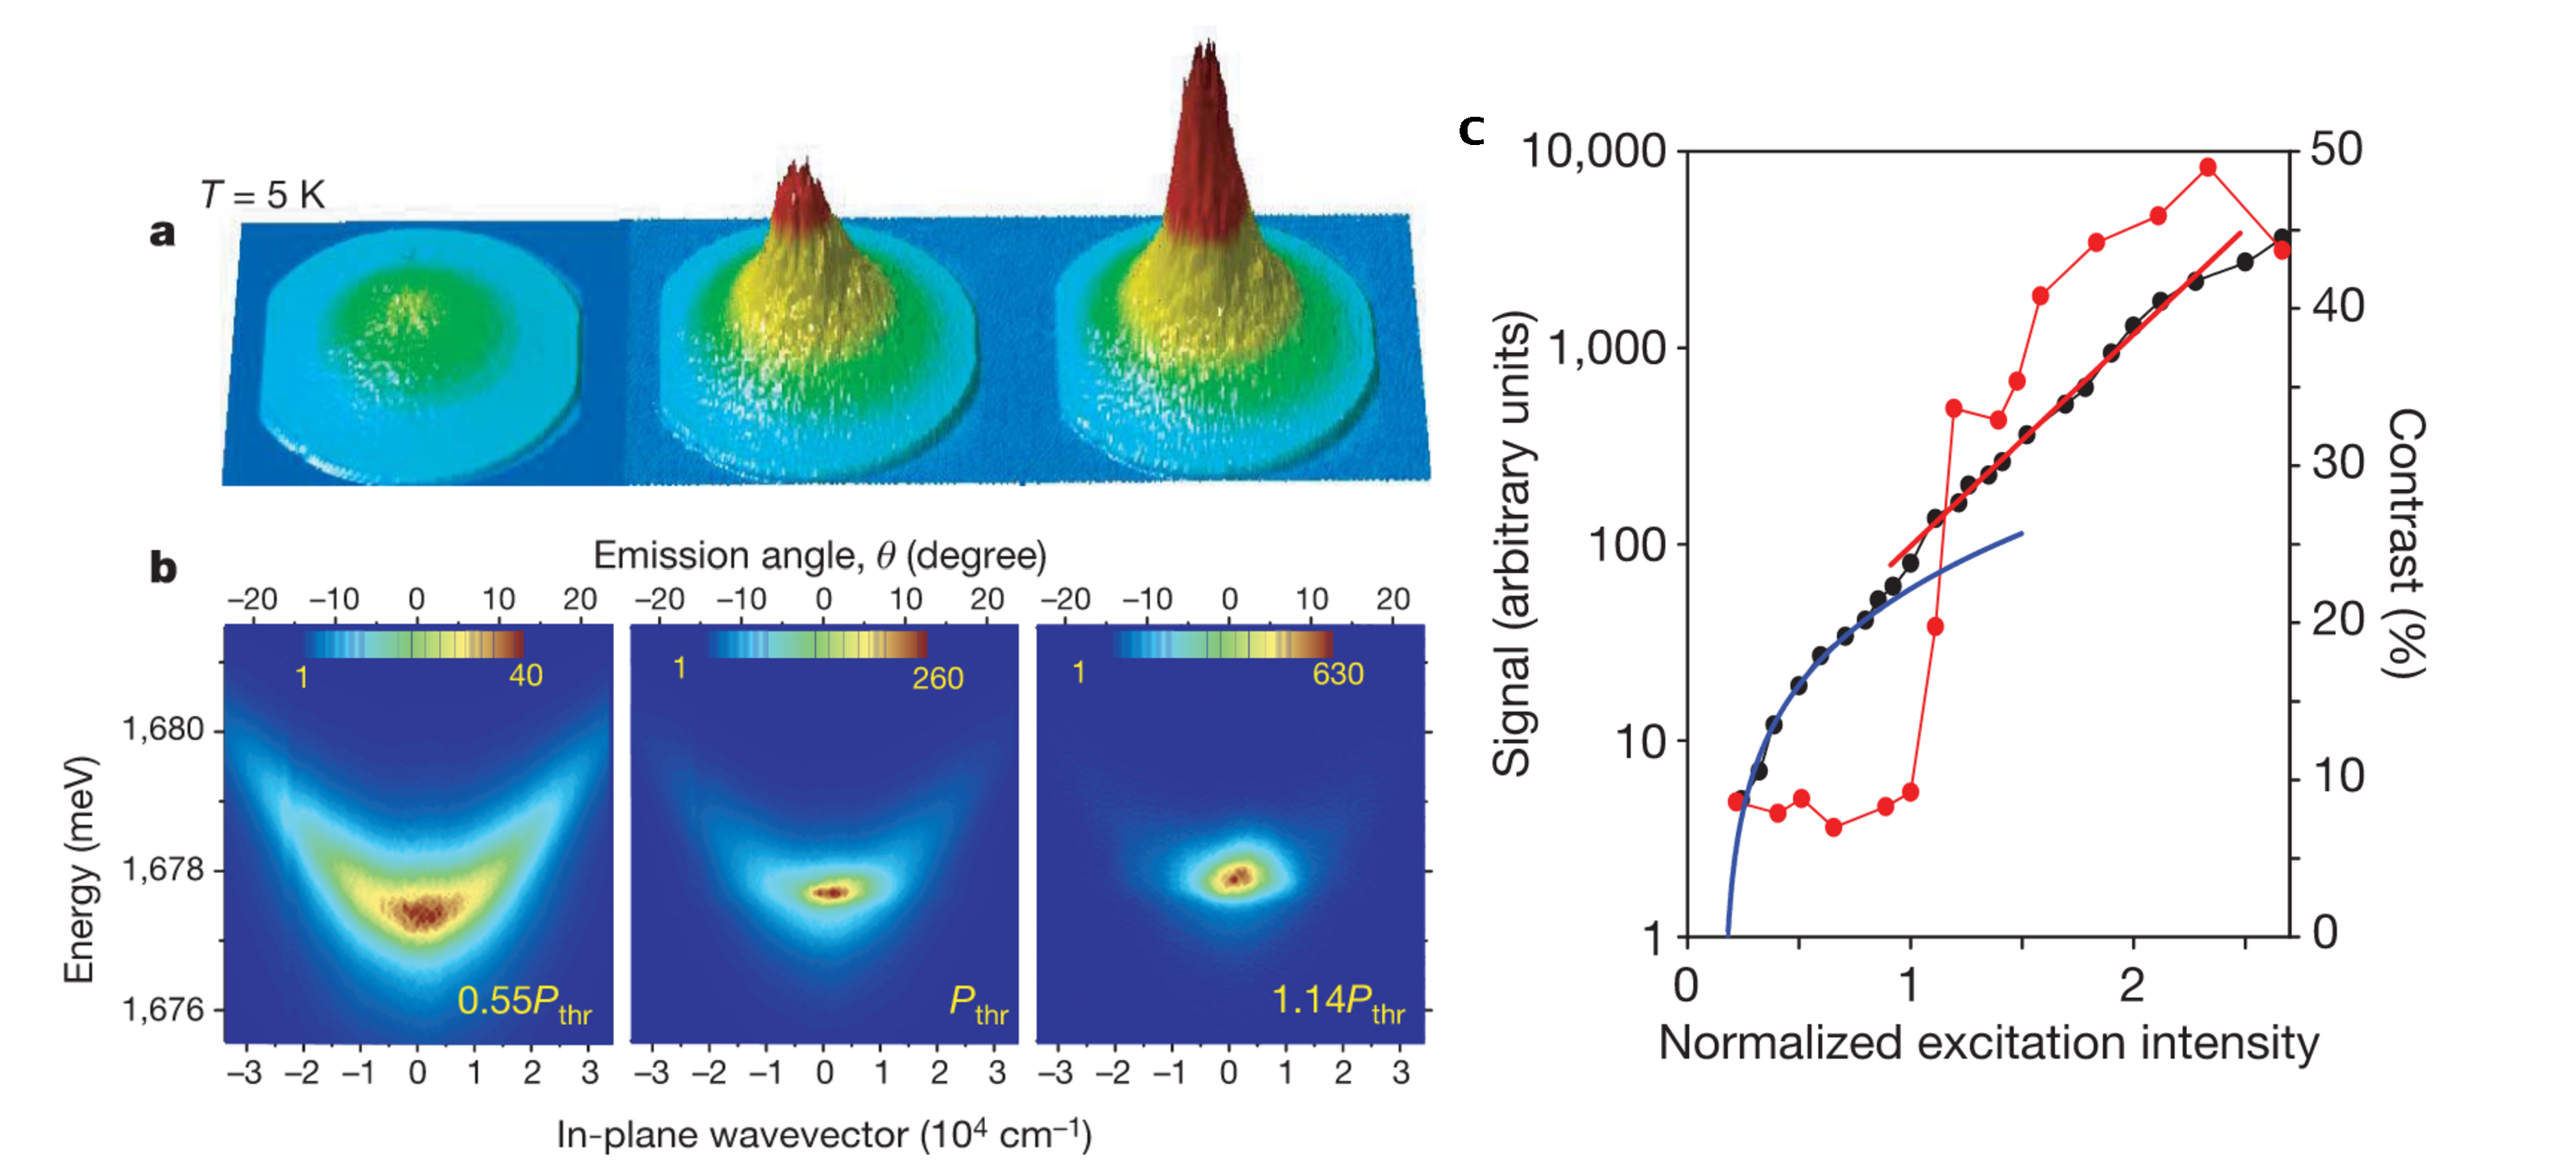
\includegraphics[width=1\linewidth]{chap_theory/fig/polariton_bec.pdf}
    \caption{\textbf{Bose-Einstein condensation of polaritons.} \textbf{a)} Far field emission of the fluid for increasing pump intensity. Above threshold, a strong emission in the zero wavevecotr mode is observed. \textbf{b)} Polariton dispersion for increasing pump intensities. Above threshold the bottom of the LP branch is macroscopically populated.
     \textbf{c)} Spatial correlation measurements using a Michelson interferometer.Solid red circles indicate correlations between two spots separated by 6mm (2.5 times the thermal de Broglie wavelength) within the condensate as a function of the excitation power. The correlation exhibits a threshold-like behaviour. 
     The variation of the ground-state emission intensity, normalized to the excitation power, is shown for comparison (solid black circles). The solid blue line is a quadratic fit of the data demonstrating the occurrence of particle-particle interaction below threshold. Above threshold, the solid red line is an exponential fit demonstrating the strong stimulation of the relaxation by the high occupancy factor of the ground state.Adapted from \cite{kasprzak_boseeinstein_2006}.}
    \label{fig:polariton_bec}
\end{figure}


\bigskip

\subsubsection{Resonant excitation.} In the resonant case, the pump laser is tuned near the polariton energy. The population of the polaritons is then directly driven by the pump laser. In particular due to momentum and energy conservation, the spatial and temporal coherence of the pump laser are transfered to the polaritons fluid. 
In that case the phase of the fluid is fixed by the pump and therefore is not randomly chosen. In this excitation scheme the fluid should then not be called a condensate. However, it can still exhibit superfluidity and other quantum fluid properties because it possesses the required properties, namely : a macroscopic occupation of a single quantum state, long range coherence and weak interactions.
In this work we will only use the resonant scheme to take advantage of the tunability of the pump to create fluid with arbitrary densities and velocity profiles. Before detailing the great versatility of this system, let us  first discuss 
a consequence of the resonant excitation scheme which will be of great interest in the following.

\textbf{Optical bistability.} Consider a Fabry-Perrot cavity filled with a non-linear Kerr medium, through which a weak resonant laser beam is shone. As the laser intensity is low, the refractive index within the cavity is the same as the bare medium. It means that the optical lenght of the cavity is an integer multiple of half the laser wavelength.
If the laser intensity is increased, the non-linear Kerr effect turns on and the refractive index of the medium increases. The laser is then no longer resonant with the cavity which reduce the intensity of the intracavity field and counteract on the refractive index. This interplay between 
non-linearities and resonance conditions is at the heart of what is called optical bistability. Since this phenomenon is not proper to polaritonic system, we will, to understand it more in details, follow the very general derivation done in \cite{grynberg_aspect_fabre}.
\label{subsec:optical_bistability}

\bigskip

\begin{figure}
    \centering
    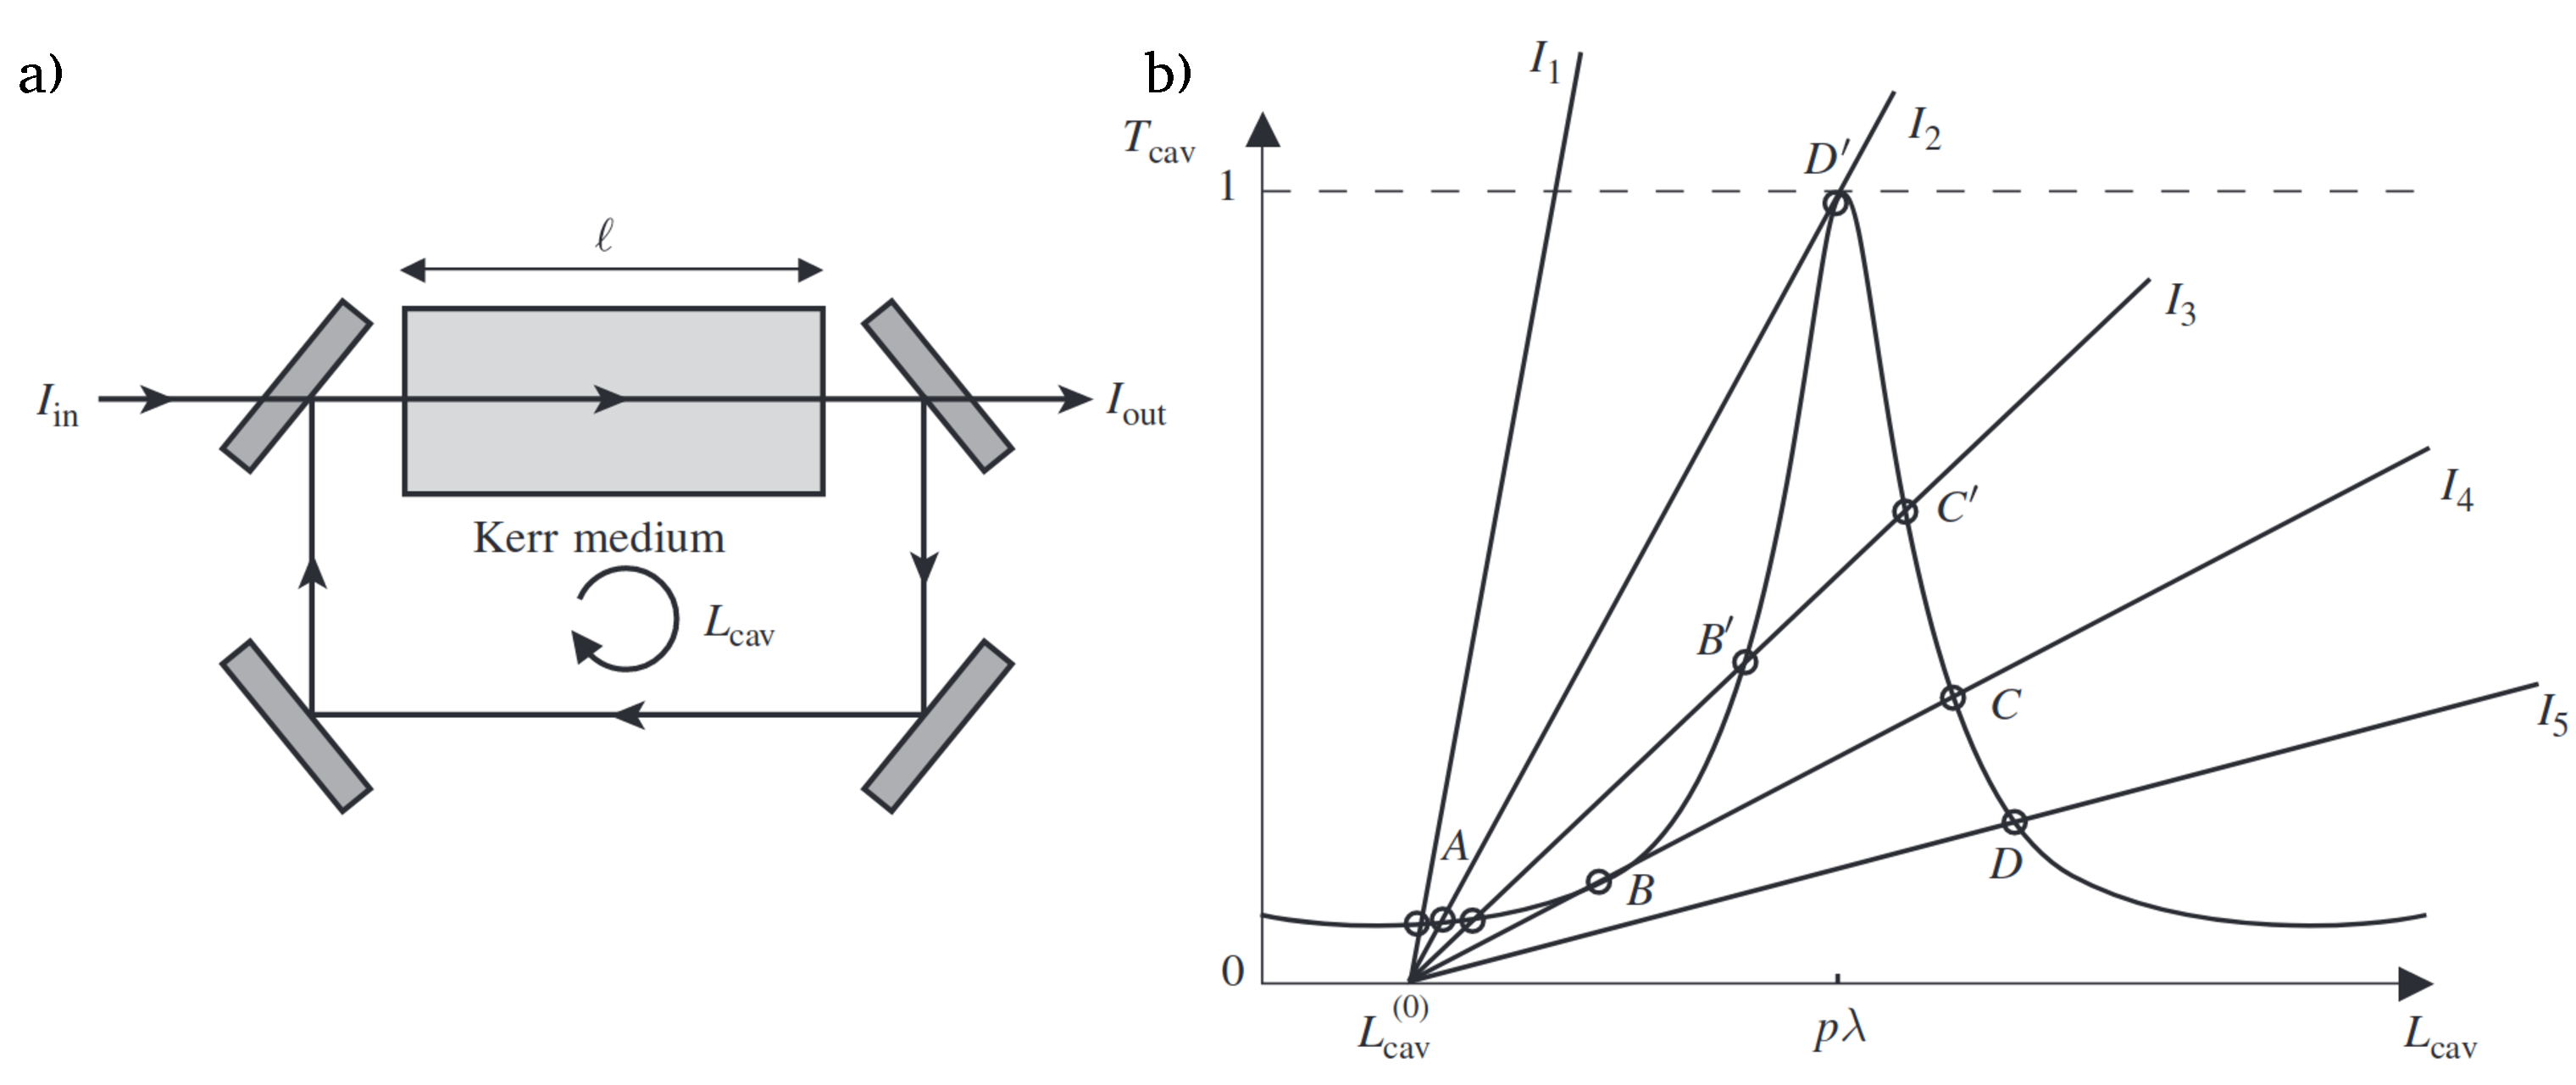
\includegraphics[width=1\linewidth]{chap_theory/fig/bistability_grynberg.pdf}
    \caption{\textbf{Optical bistability.} \textbf{a)} Schematic of a ring cavity filled with a Kerr medium. The cavity has a length $L_{cav}^{(0)}$ and the Kerr medium a length $l$. \textbf{b)} Transmission of the cavity as a function of the optical length of the cavity $L_{cav}$. The straight line represent the values $T_{cav}$ as a function of $L_{cav}$ for different values of
    $I_{in}$. The operating points lie at the intersections of the cavity resonance curve and the straigth lines. Depending on $I_{in}$ one or three operating point can be found. Adapted from \cite{grynberg_aspect_fabre}.}
    \label{fig:optical_bistability}
\end{figure}

To avoid first complications due to cross Kerr effect we consider a ring cavity of geometrical length $L$ filled with Kerr medium of lenght $l$ as shown in \autoref{fig:optical_bistability} a). The optical length of
such a cavity is :

\begin{equation}
    L_{cav}= L+(n_0-1)l+n_2I_{cav}l,
    \label{eq:optical_length}
\end{equation}
where $n_0$ is the refractive index of the medium, $n_2$ the non linear refractive index and $I_{cav}$ the intracavity intensity.
As explained for a planar cavity in \autoref{sec:photon}, the cavity has transmission peaks whenever the optical path of a round trip in the cavity (a photon going back and forth) is an integer multiple of the laser wavelength $\lambda$.
In the case of a ring cavity this condition reads as :

\begin{equation}
    T_{cav} = \dfrac{1}{1+\dfrac{4F^2}{\pi^2}\mathrm{sin}^2\left(\dfrac{kL_{cav}}{2}\right)},
    \label{eq:ring_cavity_transmission}
\end{equation}
where $F$ is the cavity finesse and $k=2\pi/\lambda$ the wavevector of the laser. The transmission of the cavity as a function of $L_{cav}$ is plotted in \autoref{fig:optical_bistability} b). 
On the other hand the transmission of the cavity is defined as :
\begin{equation}
    T_{cav} = \dfrac{I_{out}}{I_{in}}= T\dfrac{I_{cav}}{I_{in}}= \dfrac{T}{n_2l}\dfrac{L_{cav}-L^{(0)}_{cav}}{I_{in}},
    \label{eq:linear_transmission}
\end{equation}
where $T$ is the transmission of the outpout mirror and $L_{cav}^{(0)}$ the optical length of the cavity at low intensity $I_{cav}\approx 0$. An operating point is then defined as the intersection of the transmission curve \autoref{eq:ring_cavity_transmission} and the straight line of \autoref{eq:linear_transmission}. Graphically the slope 
of the linear relation between $T_{cav}$ and $L_{cav}$ depend on the value of $I_{in}$.
As a consequence several regime are possible depending on the value of the input intensity as shown in \autoref{fig:optical_bistability} b). For low intensity as $I_1$, the operating point is unique and the system is in a stable regime but yields a low transmission. For higher input intensity like $I_3$, the system exhibits three operating points. However, it can be shown that the intersection points with a negative derivative between B and D are unstable. At even higher 
intensity the system has again a single operating point and a poor transmission. When the input intensity lies between $I_2$ and $I_4$ the system is said to be in a bistable regime. 

\bigskip 

In the case of microcavity-polariton the same behavior can be observed as the exciton-exciton non-linear interactions are of the same nature as the Kerr effect.
Analytically, polariton bistability can be found by looking at the steady state of the driven-dissipative Gross-Pitaevskii equation in the presence of a driving pump term nearly resonant with the LP branch. In first approximation, it can be written as a plane wave $F_p(\rvec,t)=F_p e^{i\kvec_p.\rvec-i\omega_p t}$.
As it is usually done for equations including a resonant forcing term, we look for solution of the same form namely, plane wave with the same phase, $\psi(\rvec,t)= \sqrt{n_0}e^{i\kvec_p.\rvec-i\omega_p t}$.
Inserting this ansatz into \autoref{eq:generalized_GPE} in the absence of external potential $V_{LP}=0$ one obtain the steady state equation :

\begin{equation}
    \left[\omp -\omlp - \dfrac{\hbar \kp^2}{2 \mlp} - g n_0 - g_rn_r + i \dfrac{\gamlp}{2} \right] \sqrt{n_0}= \eta_{LP} F_p^0,
    \label{eq:steady_state}
\end{equation}
while the reservoir rate equation gives :
\begin{equation}
    n_r = \dfrac{\gamma_{in}}{\gamma_r}n_0.
\end{equation}
To eliminate the reservoir density we follow the procedure done in \cite{stepanov_dispersion_2019} and introduce an effective interaction strenght $g_{e}=g+g_r\frac{\gamma_{in}}{\gamma_r}$ so that $g_rn_r+gn=g_{e}n$. 
We can then rewrite \autoref{eq:steady_state} as :
\begin{equation}
    \left[\omp -\omlp - \dfrac{\hbar \kp^2}{2 \mlp} - g_{e}n_0 + i \dfrac{\gamlp}{2} \right] \sqrt{n_0}= \eta_{LP} F_p^0.
    \label{eq:steady_state_2}
\end{equation}
It is the equivalent of the equation of state of a conservative system with the difference that, in this case, it results of a complex equilibrium between interactions, pumping and losses. Notice that 
the contribution of the dark reservoir just appear as a correction on the interaction strength and thus doesn't change much the phenomenology discussed earlier. Nonetheless, it 
 has quantitative consequences on the hysteresis cycle that can be used to probe polariton-dark excitons interactions with optical means, notably through two photon excitation to overcome spin forbidden transitions \cite{dark_exciton_pol_interactions}

\bigskip

To end up with an equation linking the pump intensity to the polariton density one can multiply this equation by its complex conjugate which gives :

\begin{equation}
    n \left[ \dfrac{\gamlp^2}{4} + \left(\delta(\kp) - g_{e} n \right)^2 \right] =  \eta_{LP}^2 I,
\label{eq:eq_of_state}
\end{equation}

where $\delta(\kp)$ is the effective detuning between the pump laser and the LP branch at the pump wavevector in a parabolic approximation, $\delta(\kp) = \omp - \omlp-{\hbar\kp^2}/2\mlp$ and $I$ the pump intensity. Being a polynomial of degree 3 in the polariton density, this equation have up to three solutions.
Three distinct real solutions can be found only if $\delta>\sqrt{3/2}\gamlp$, as explained in the previous paragraph, one of this solution is known to be unstable. However, in some peculiar cases, namely when the fluid dimension is ramped down from 2D to 1D this solution can be explored and is responsible for the emergence of first order phase transition as investigated in \cite{li_dissipative_2022}.
This being said, we don't take into account this solution in the present work since the dimension of the fluid will always be 2D.
The evolution of $n$ as a function of $I$ in this regime is plotted in \autoref{fig:bistability}. The system is in a bistable regime when the curve exhibits two stable solutions for a given intensity : one at low density and one at high density.
It's worth noticing that the actual state in which the system is depend on its past history. More precisely, if the incident intensity is initially low, since the laser is blue detuned with the polariton energy, the photon injection whithin the sample is poor and a few polariton are created. However, their presence in the cavity tends to blueshift their own resonance energy as explained in \autoref{sub:polariton_interactions}. As the intensity is ramped up, the system will follow the low density branch until the energy renormalisation is sufficient to reach the point B. At this point the system is compelled to jump to the high density branch and will suddenly move from point B to point C.
If the pump intensity is then decreased, the situation is rather different since many polaritons are already present in the sample and support the laser injection and thus polariton creation. The system will follow the high density branch untill it reaches the point D' where interactions can no longer compensate for the losses making it fall again on the low density branch. A particular attention must be given to this so called turning point D'. Indeed, as it can be seen on \autoref{fig:optical_bistability} it's the only point at which the laser is exactly resonant with the cavity filled with non linearities.
This point can only be reached by travelling on the whole hysteresis loop. The corresponding density can determined by solving $\frac{dI}{dn}=0$ which gives the discriminants :

\begin{equation}
    \Delta = g_{e}^2 \left( \delta^2 - \dfrac{3\gamlp^2}{2}\right).
\end{equation}

The bistable regime require two distinct solution for $\frac{dI}{dn}=0$ which require $\Delta>0$ and provide the afromentionned condition $\delta>\sqrt{3/2}\gamlp$.
From this one can find that the density corresponding to the turning point fulfill $\delta(\kp)=g_{eff}n = gn_0+g_rn_r$. 

\begin{figure}
    \centering
    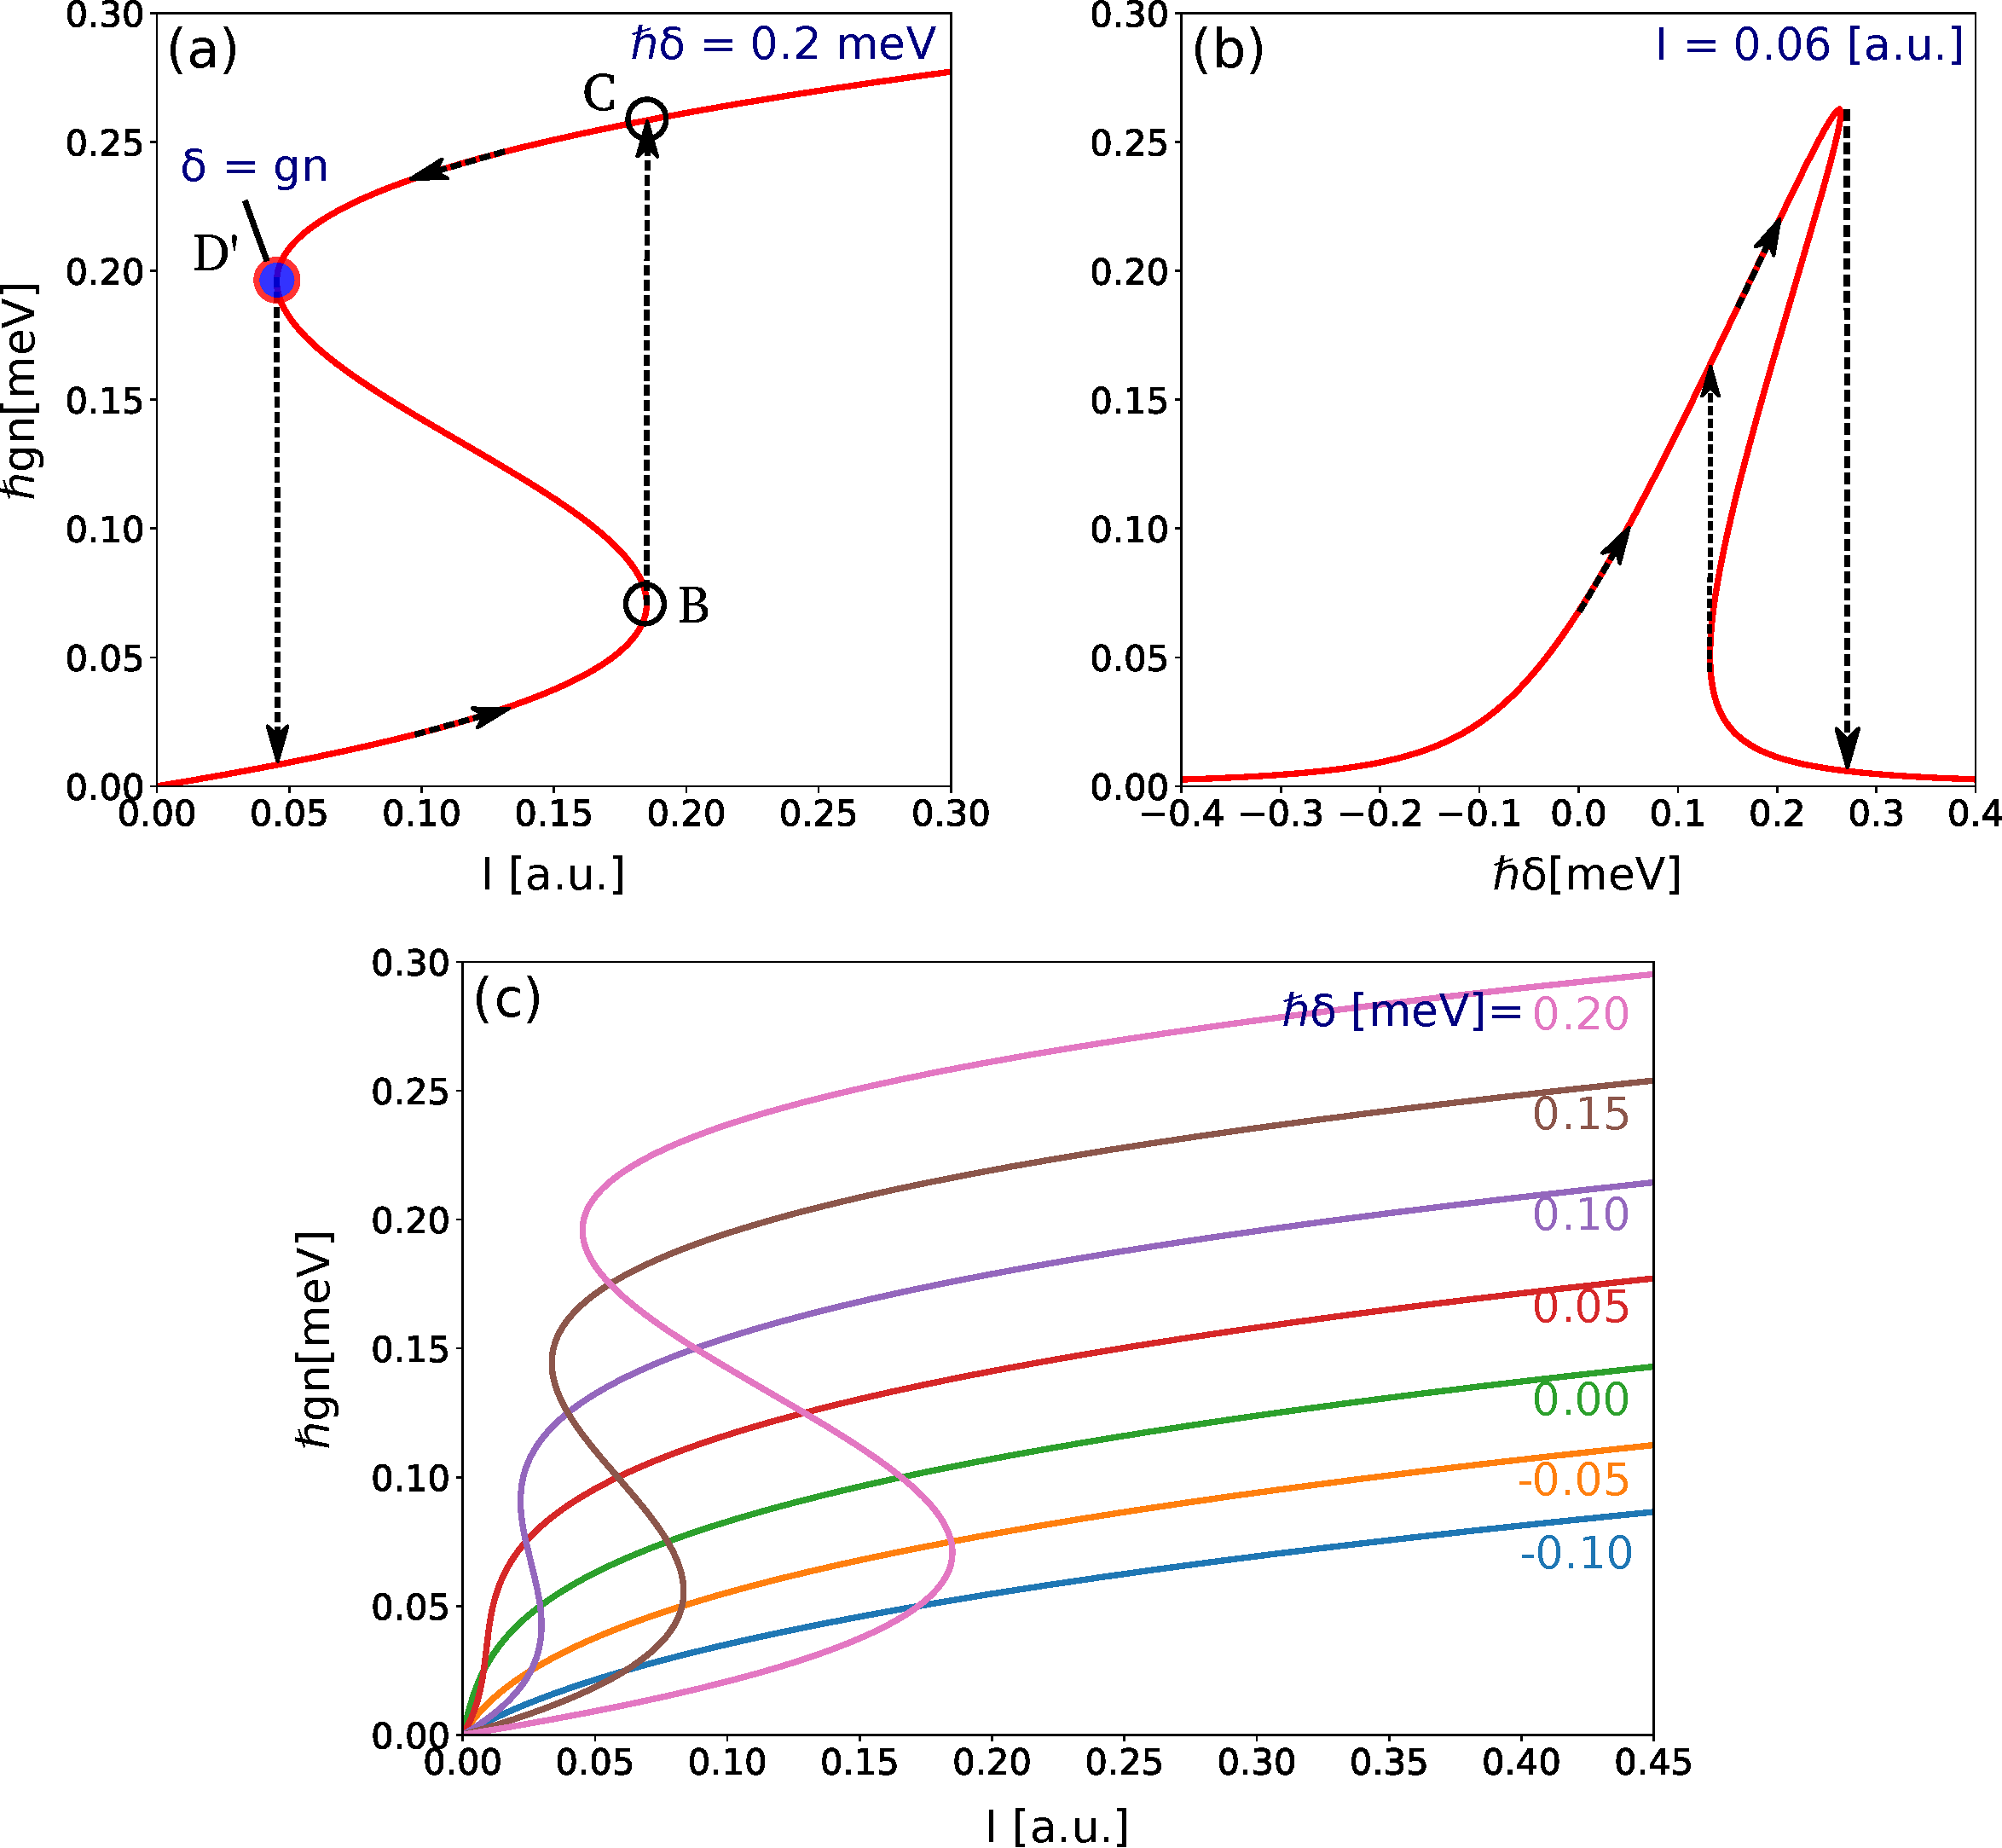
\includegraphics[width=0.8\linewidth]{chap_theory/fig/bistability.pdf}
    \caption{\textbf{Optical bistability in a polariton fluid.} \textbf{a)} The polariton density as a function of the pump intensity when $\delta>\frac{\sqrt{3}\gamlp}{2}$. The blue point represent the so called turning point at which the detuning is exactly equal to the interaction energy.
    \textbf{b)} Polariton density as a function of $\delta$ for a fixed pump intensity. c) Polariton density as a function of the pump intensity for different values of $\delta$, bistability is observed when $\delta>\frac{\sqrt{3}\gamlp}{2}$.}
    \label{fig:bistability}
\end{figure}

Conversely, when the detunig is two small with respect to the system losses the system is monostable and said to be in the optical limiter regime.
In the bistable regime, the system exhibits 


\textbf{All optical control.} In the context of analog gravity, the ability to easily control and monitor the fluid of light is a great asset. Indeed, the study of 
Hawking radiation in a quantum fluid require the creation of an acoustic horizon as well as the possibility to measure what is emitted by the latter. In particular,
it is crucial to achieve two goals. 

\begin{itemize}
    \item 1. Create and monitor a stable fluid with an arbitray flow profile and density since the mean field and especially its velocity profile are the analog of the curved spacetime we want to study.
    \item 2. Probe the fluid collective excitations. These small perturbations on top of the mean field are the fluid counterpart of the quantum fields fluctuations considered in the Hawking radiation theory.
\end{itemize}

With planar microcavity polaritons this is done fully optically since the fluid is created by the pump laser and is monitored by collecting the photons leaving the sample. 
The first point is allowed by the resonant excitation scheme. The velocity of a polariton being $\mathbf{v_{LP}}=\frac{\hbar \kvec_{LP}}{\mlp}$ momentum conservation enable to create a fluid with a given velocity by just changing the pump incidence angle (see \autoref{sec:photon}).
This correspondance also holds for the light outgoing the sample : the recombination of a polariton with wavevector $\kvec$ produce a photon with the same wavevector. 
Although the relation between the pump intensity and the polariton density is not trivial as we shall see in the next section, it is also a practical control knob that can be used to tune the fluid speed of sound.
The second point can again be tackled with optics means since the struture of collective excitations is ultimately hidden in the fluctuations of the photonic field outgoing the sample. As a consequence, the large
variety of tools and methods developped in the field of optics can be used to probe the fluid. Microcavity polaritons, are liying at the crossroad of optics and quantum fluids, definitely justifying the designation "quantum fluid of light".



% !TeX encoding = UTF-8
% !TeX spellcheck = fr_FR
% !TeX root = ../mythesis.tex
% !TeX program = pdflatex (build)
%%% TeXmaker : no 'magic comments' but set Root with Options > Set as master file

%useful stuff for what follows
\newcommand{\xbf}{\pmb{x}}
\newcommand{\ci}{\mathrm{i}}
\newcommand{\ee}{\mathrm{e}}
\newcommand{\lr}[1]{\left(#1\right)}
\newcommand{\lrsq}[1]{\left[#1\right]}
\newcommand{\tp}{\mathrm{p}}
\newcommand{\tv}{\mathrm{v}}
\newcommand{\vtv}{\boldsymbol{\mathrm{v}}}
\newcommand{\vna}{\boldsymbol{\nabla}}
\newcommand{\vx}{\mathbf{x}}
\newcommand{\tx}{\mathrm{x}}
\newcommand{\vobf}{\pmb{v_0}}
\newtheorem{theorem}{Theorem}
\newtheorem{lemma}[theorem]{Lemma}

\newcommand{\kbf}{\mathbf{k}}
\newcommand{\vbf}{\pmb{v}}
\newcommand{\rbf}{\mathbf{r}}
\newcommand{\ombog}{\omega_{\mathrm{b}}}
\newcommand{\betin}{\beta^{\mathrm{in}}}
\newcommand{\betout}{\beta^{\mathrm{out}}}
\newcommand{\rmexp}{\mathrm{exp}}
\newcommand{\im}{\mathfrak{Im}}
\newcommand{\re}{\mathfrak{Re}}
\newcommand{\mbogo}{m_{\mathrm{det}}}
\newcommand{\cs}{c_{\mathrm{s}}}
\newcommand{\dpsi}{\delta\psi}
\newcommand{\opsi}{\hat{\psi}}
\newcommand{\odpsi}{\hat{\delta\psi}}
% \newcommand{\norm}[1]{\left\lVert#1\right\rVert}
\newcommand{\dr}{\mathrm{d}\mathbf{r}}
\newcommand{\Lbog}{\mathcal{L}_B}
\newcommand{\ha}{\hat{a}}
\newcommand{\hadag}{\hat{a}^\dagger}
\newcommand{\hb}{\hat{b}}
\newcommand{\hbdag}{\hat{b}^\dagger}

\setcounter{topnumber}{2}
\setcounter{bottomnumber}{0}
\setcounter{totalnumber}{2}
\renewcommand{\topfraction}{0.99}
\renewcommand{\textfraction}{0.01}
\renewcommand{\floatpagefraction}{0.8}


\graphicspath{{./}{./fig/}{./chap_Ag_theory/fig/}}

\chapter{Hawking radiation in a polariton quantum fluid}
\label{chap:AG_theory}

Now that polaritons have been introduced, we can start to discuss the theoretical framework that will be used to 
describe Hawking radiation in a polariton quantum fluid. In this chapter, we will first establish the original hydrodynamical analogy between the propagation 
of acoustic waves in a moving fluid and scalar fields in curved spacetime. This analogy is at the heart of what motivated the study 
of Hawking radiation in analog systems, leading to a first variety of experiment in classical systems such as water tanks. These great experiments,
\cite{rousseaux_observation_2008,weinfurtner_measurement_2011} demonstrated positive to negative frequency conversion of shallow surface waves at the vicinity of a sonic horizon. However the temperature
of classical fluids is too high to quantize their collective excitation field which prevent the study of quantum effects. More precisely, Hawking radiation is expected 
to create entanglement between the emitted modes which can not be tested with water waves. Quantum fluids appear then as promising candidate since the 
fluctuations around the ground or steady state require a quantum treatment to be understood. In fact we will see that tackling a fluid with trans-critical flow with the usual Bogoliubov theory of condensed matter also predict particle creation from vacuum. Studying the effect from this point of view will reveal a strong robustness 
of the effect beyond the original hydrodynamical approach and widen the range of regimes where Hawking radiation can be observed.


\section{The hydrodynamical analogy}

In the previous chapter, we established that the dynamics of microcavity polaritons can be described by a driven dissipative Gross-Pitaevskii equation.
By writing the wavefunction in term of phase and density the Gross-Pitaevskii equation can be cast into a continuity equation and an Euler equation for a non-barotropic fluid in the pump rotating frame. Starting from the GPE
a system pumped by a laser of the general form $F_{\tp}e^{i\phi(x,t)}$ lead the fluid to a stationnary state whose wavefunction $\psi(x,t)=\sqrt{n_0}e^{i\phi(x,t)}$ phase and modulus respect :
\begin{equation}
    \begin{align}
    \partial_t \phi +& \frac{\mlp v_0^2}{2\hbar}+\frac{\hbar}{2\mlp}\frac{\partial_x^2\sqrt{n_0}}{\sqrt{n_0}}+V_{LP}+gn+g_rn_r+\frac{\re\lrsq{F_{\tp}e^{-i\theta}}}{\mlp}=0\,\\
    \partial_t n_0 +& \partial_x(n_0v)= \gamma n_0 -2\im\lrsq{F_{\tp}e^{-i\theta}}\sqrt{n_0}
    \end{align}
    \label{eq:continuity}
\end{equation}
If we neglect the pump and dissipation terms which is basically the situation of a conservative fluid, we recover the original equation describing 
sound waves in a convergent flow. This is precisely the equation that was used in the initial analogy made by W. Unruh \cite{unruh_experimental_1981}.
However, the out of equilibrium nature of the microcavity polaritons brings different phenomenology. In particular, perturbations propagating in
the fluid are not necessary sound waves as we will se latter. It means that the dispersion of these perturbation is not linear and 
can remarkably exhibit a gap which can be associated to massive excitations. To avoid making approximation and encapsulate as much as possible 
the complexity of the system it is convenient to make the same calculation in the pump rotating frame. It equivalently means that all frequencies
will be taken with respect to the pump. In practice this is done by writting the pump $F_{\tp}(x)= F_{\tp}e^{i\theta_p(x)}$ and look for steady state wavefunction 
of the same form $\psi(x,t)=\sqrt{n_0}e^{i\theta_p(x)}$. Plugging this into the GPE we obtain that the phase and density of the fluid must fullfill the following equations :

\begin{equation}
    \lrsq{-\frac{\hbar}{2\mlp}\nabla^2-i\frac{\hbar}{2}(\vna\cdot\pmb{v_0}) -i\hbar(\pmb{v_0}\cdot\vna)- \delta(v_0)+g_{\rm r}n_{\rm r}+g n_0-\ci\frac{\hbar\gamma}{2}}\sqrt{n_0}+|F_\tp|=0\,,
        \label{eq:StatHomogEOSDens}
\end{equation}
with $\hbar \delta(v_0)=\hbar\omega_\tp-\hbar\omega_0-\mlp v_0^2/2$ (note that this is just $\delta(k_p)$ in a homogeneous configuration where $\pmb{v_0}=\hbar\pmb{k_p}/\mlp$).
To study the low energy collective perturbations of the fluid state we linearize the system around the steady state by writing the wavefunction
$\psi(x,t)=(\sqrt{n_0}+\delta\psi(x,t))e^{i\theta_p(x)}$. Injecting this expression in \autoref{reservoir_eq} and using \autoref{eq:StatHomogEOSDens} we obtain at linear order in $\delta\psi$ :

\begin{equation}
    \ci \hbar \lr{\partial_t+\pmb{v_0}\cdot{\vna}}\delta\psi=\lrsq{-\frac{\hbar}{2m^*}\nabla^2+\rho-\ci\sigma}\phi+g n_0 \delta\psi^*,
        \label{eq:DefPertGPE}
\end{equation}
where $$\rho\coloneqq2g n_0- \delta(v_0)+g_{\rm r}n_{\rm r}\qquad\text{and}\qquad\sigma\coloneqq\hbar/2\vna \cdot\pmb{v_0}.$$
Note that here we have assumed that there is no external potential without loss of generality since it can be included in the definition of $\rho$.


\section{At the heart of particle creation : Bogoliubov transformation}

\subsection{The ambiguity of vacuum definition}
The quantum vacuum state is defined as the quantum state of a system with the lowest possible energy. Eventhough 
this definition is commonly used and looks quite intuitive, it in fact implies some deep properties. First, a minimum energy state exists. In a finite dimension
problem, this is obvious since the spectrum has also a finite dimension but whenever the dimension of the Hilbert space is infinite, the existence of a minimum energy state is a priori not guaranteed.
Secondly, it seems to depend on the system which suggests that the vacuum is not a universal concept. This is particularly true in the context of quantum field theory in curved spacetime where the vacuum state is observer dependent.
For instance, in the Unruh effect, an accelerating observer detect a thermal radiation while an inertial observer sees 'standard' vacuum. This ambiguity is
as at the root of particle creation phenomena like the Hawking effect and once it is understood, make these effects appear less surprising.


\subsubsection{The harmonic oscillator}

To start with, let us consider the usual harmonic oscillator describing a massive particle in a one dimensionnal harmonic potential and
see how the defintion vacuum arise in this simple case \cite{CCT_tome1}. The Hamiltonian of the particle of mass $m$ is :


\begin{equation}
    H=\frac{P^2}{2m}+\frac{1}{2}m\omega^2X^2
\end{equation}
Where $P$ and $X$ are the momentum and position operators satisfying the canonical commutation relation $[X,P]=i\hbar$.
It is convenient to define the dimensionless operators :

\begin{subequations}
    \begin{align}
        \hat{P}&=\frac{1}{\sqrt{\hbar m\omega}}P,\\
        \hat{X}&=\sqrt{\frac{m\omega}{\hbar}}X, 
    \end{align}
\end{subequations}
which respect the commutation relation $[\hat{X},\hat{P}]=i$. The Hamiltonian is then written as :
\begin{equation}
    H=\hbar\omega\hat{H}
\end{equation}
with :
\begin{equation}
    \label{eq:dimensionless_hamiltonian}
    \hat{H}=\frac{1}{2}\lr{\hat{P}^2+\hat{X}^2}.
\end{equation}
The corresponding eigenproblem is usually tackled by introducing the creation and annihilation operators :

\begin{subequations}
    \begin{align}
        \hat{a}&=\frac{1}{\sqrt{2}}\lr{\hat{X}+i\hat{P}},\\
        \hat{a}^\dagger&=\frac{1}{\sqrt{2}}\lr{\hat{X}-i\hat{P}},
    \end{align}
\end{subequations}
which satisfy the commutation relation $[\hat{a},\hat{a}^\dagger]=1$.
Taking the definition of $\hat{a}$ and $\hat{a}^\dagger$ we look a the quantity $\hat{a}^\dagger\hat{a}$ :

\begin{equation}
    \begin{align}
    \hat{a}^\dagger\hat{a}&=\frac{1}{2}\lr{\hat{X}-i\hat{P}}\lr{\hat{X}+i\hat{P}} \\
                          &=\frac{1}{2}\lr{\hat{X}^2+\hat{P}^2+i\lr{\hat{X}\hat{P}-\hat{P}\hat{X}}} \\
                          &=\frac{1}{2}\lr{\hat{X}^2+\hat{P}^2-1}.
    \end{align}
\end{equation}
Comparing with \autoref{eq:dimensionless_hamiltonian} we see that :

\begin{equation}
    \label{eq:ham_number_operator}
    \hat{H}=\hat{a}^\dagger\hat{a}+\frac{1}{2}.
\end{equation}
We then naturally introduce the operator $\hat{N}=\hat{a}^\dagger\hat{a}$. Eventhough this operator 
is known to be the number operator, we will on purpose treat it without prior knowledge and see what can be learned from the derivation.
From \autoref{eq:ham_number_operator} we see that the an eigenstate $\ket{\phi^i_\nu}$ of $\hat{N}$ with eigenvalue $\nu$ is also
an eigenstate of $\hat{H}$ with eigenvalue $\nu+\frac{1}{2}$. Solving the problem then boils down to find the spectrum of $\hat{N}$.

\textbf{Spectrum determination.} The operator $\hat{N}$ is hermitian and its eigenstates form a complete basis of the Hilbert space. Let us 
show two usefull lemmas resulting directly from the definition of $\hat{N}$ :

\begin{lemma}
    The eigenvalues of $\hat{N}$ are positive or zero.
\end{lemma}

\begin{proof}
    Let us consider any eigenstate $\ket{\phi_\nu}$ of $\hat{N}$. The square of norm of the state $\hat{a}\ket{\phi_\nu}$ is 
    \begin{equation}
            \norm{\hat{a}\ket{\phi_\nu}}^2=\bra{\phi_\nu}\hat{a}^\dagger\hat{a}\ket{\phi^i_\nu} \geq 0   
\end{equation}
    Using the definition of $\hat{N}$ we have :
    \begin{equation}
        \label{eq:positive_eigenvalue}
        \bra{\phi_\nu}\hat{a}^\dagger\hat{a}\ket{\phi_\nu}=\nu\bra{\phi_\nu}\ket{\phi_\nu} \geq 0.
    \end{equation}
Since $\bra{\phi_\nu}\ket{\phi_\nu}>0$ we have $\nu\geq 0$.
\end{proof}

\begin{lemma}
    Let $\ket{\phi_\nu}$ be an eigenstate of $\hat{N}$ with eigenvalue $\nu$.
    \begin{itemize}
        \item \ $\nu=0$ if and only if $\hat{a}\ket{\phi_\nu}=0$.
        \item If $\nu>0$ then $\hat{a}\ket{\phi_\nu}$ is an eigenstate of $\hat{N}$ with eigenvalue $\nu-1$.
    \end{itemize}
\end{lemma}

\begin{proof}
    If $\nu=0$, \autoref{eq:positive_eigenvalue} implies that $\bra{\phi_\nu}\ket{\phi_\nu}=0$ which imposes that $\ket{\phi_\nu}=0$.
    Reciprocally, if $\hat{a}\ket{\phi_\nu}=0$ a multiplication by $\hat{a}^\dagger$ gives $\hat{N}\ket{\phi^i_\nu}=0$. Since $\ket{\phi_\nu}$ is not zero we conclude
    that $\ket{\phi_\nu}$ is an eigenvector of $\hat{N}$ with eigenvalue $\nu =0$.

    COnsider now that $\nu>0$, we now know that $\hat{a}\ket{\phi_\nu}$ is not zero. By using the identity $\bigl[\hat{N},\hat{a}\bigr] = -\hat{a}$ we 
    obtain :
    \begin{equation}
        \hat{N}\hat{a}\ket{\phi_\nu}=\hat{a}\hat{N}\ket{\phi_\nu}-\hat{a}\ket{\phi_\nu}=(\nu-1)\hat{a}\ket{\phi_\nu},
    \end{equation}
    which shows that $\hat{a}\ket{\phi_\nu}$ is an eigenstate of $\hat{N}$ with eigenvalue $\nu-1$.
\end{proof}

\noindent Let us summarize what we know so far :
\begin{itemize}
    \item The operator $\hat{N}$ has a non negative spectrum. 
    \item If $\nu$ is an eigenvalue of $\hat{N}$ then $\nu-1$ is also an eigenvalue of $\hat{N}$.
\end{itemize}

This two properties are in fact sufficient to show that the spectrum of $\hat{N}$ are the positive or zero integers. \\
\bigskip 

Assume, by contradiction, that there is a positive non integer eigenvalue $\nu$ associated with the eigenvector $\ket{\phi_\nu}$ . Then, by the second lemma, $\nu-1$ is also a non integer eigenvalue of $\hat{N}$ generated by 
the action of $\hat{a}$ on $\ket{\phi_\nu}$. By iterating this process we obtain a sequence of eigenvalues $\nu,\ \nu-1,\ \nu-2,\dots$ which is impossible since the spectrum is bounded from below. More precisely, it exists
a positive integer $p$ such that $\nu-p<0$ which contradicts the fact that the spectrum is non negative. We conclude that the spectrum of $\hat{N}$ is the positive or zero integers.




\section{Elementary excitations of the fluid : Bogoliubov theory}
Unlike in classical systems, where Hawking radiation can only be triggered by external disturbances, its analog in quantum fluids may instead arise from vacuum fluctuations. In this context, perturbations of the quantum fluid are emitted at the horizon and propagate in opposite directions, mirroring the behavior expected near a gravitational event horizon. 
However, while the analogy with black hole physics is supported by the fact that the systems can be described by the same equation, derived in the  hydrodynamical context, nevertheless it should be noted that the systems are very different.

Indeed, treating the collective excitations of a transonic Bose-Einstein condensate within the framework of Bogoliubov theory already predicts the spontaneous emission of modes at the horizon from vacuum fluctuations. Fundamentally, both Stephen Hawking's original calculation and its quantum fluid analog rely on a Bogoliubov transformation between two sets of operators \cite{hawking_black_1972}, which ultimately leads to the mixing of creation and annihilation operators.

This section will establish the structure of the collective excitation spectrum and demonstrate how specific fluid configurations can give rise to mode emission from vacuum. Furthermore, we will show that the Hawking effect remains robust even when deviating from the original hydrodynamical analogy, and it does not necessarily require the excitations to be sound waves. 
In fact, the intrinsically out-of-equilibrium nature of the polariton system reveals a phenomenology far richer than that of conservative systems, extending the possibility of observing Hawking radiation to massive excitations.



\subsection{Linearization of the Gross-Pitaevskii equation}
\label{sec:bogo_modes_derivation}
Let us consider a monochromatic pump described by a plane wave $F_{\tp}(\rbf,t)=F_{\tp}e^{i(\kbf_p \rbf -\omega_pt)}$. As explained in the previous chapter, this will drive the system
to a steady state of the form $\psi_0(\rbf,t)=\psi_0e^{i(\kbf_p \rbf -\omega_pt)}$ and respecting :

\begin{equation}
    \left[\omp -\omlp - \dfrac{\hbar \kp^2}{2 \mlp} - g \abs{\psilp^0}^2 + i \dfrac{\gamlp}{2} \right] \psilp^0= \eta_{LP} F_p^0.
    \label{eq:steady_state}
\end{equation}

We now look for the elementary excitations following the Bogoliubov prescription which consists in linearizing the GPE around $\psi_0$. We write the wavefunction as :

\begin{equation}
    \psi(\rbf,t)=\biggl[\psi_0(\rbf)+\dpsi(\rbf,t)\biggr]e^{i(\kbf_p \rbf -\omega_pt)}.
    \label{eq:linearization_ansatz}
\end{equation}

The second term in this writing can be interpreted as the polaritons that are not in the steady state and therefore have a global phase different from the pump. 
This imply that they can have different energy and momentum that the fluid and undergo scatterings or spontaneous effects since their dynamics is not fixed by the pump. It is 
worth noticing that this term do not originate from the out of equilibrium nature of the system and would be not zero even at zero temperature due to interactions.
In the case of Bose Einstein condensates, this linearization process actually introduces a state that is not physical in the sense that it suggest the breaking of the $U(1)$ symmetry of the system or equivalently 
 that the condensates picked a phase \cite{castin_bose-einstein_2001}. The physical state is recovered through a statistical mixtures of all these "symetry broken states" which then rather appear 
as intermediate state convenient for calculation. In the case of a polariton fluid pumped quasi resonantly the situation is different since the mean field phase 
is fixed by the pump. 

\bigskip

Injecting \autoref{eq:linearization_ansatz} in the GPE, using \autoref{eq:steady_state} and keeping only the linear terms in $\dpsi$ we obtain :

\begin{equation}
    \begin{split}
        i  \hbar \partial_t \dpsi =& \biggl(\hbar\omlp^0 - \hbar \omp-\dfrac{\hbar^2}{2\mlp}\left[\nabla^2 +2i\kbf_p\nabla-\kbf_p^2\right]+\hbar g_rn_r + 2\hbar g \abs{\psi_0}^2+ \dfrac{i\hbar\gamma}{2} \biggr) \dpsi \\
                                    &+ \hbar g \psi_0^2 \dpsi^*. 
    \end{split}
    \label{eq:bogo_v1}
\end{equation}

Yet, this equation is not stricly speaking linear in $\dpsi$ since there is a term involving its complex conjugated $\dpsi^*$. A way to solve this problem
is to decompose $\dpsi$ in its real and imaginary part and to obtain two independant equations. An equivalent procedure, more common in the litterature, is to find an equation on 
the complex conjugated and consider $\dpsi^*$ as an independant variable. This is the approach we will follow here. The equation on $\dpsi^*$ is obtained by simple complex conjugation of \autoref{eq:bogo_v1} :

\begin{equation}
    \begin{split}
    -i  \hbar \partial_t \dpsi^* = &\biggl(\hbar\omlp^0 - \hbar \omp-\dfrac{\hbar^2}{2\mlp}\left[\nabla^2 -2i\kbf_p\nabla-\kbf_p^2\right]+\hbar g_rn_r + 2\hbar g \abs{\psi_0}^2- \dfrac{i\hbar\gamma}{2}\biggr) \dpsi^* \\
      &+ \hbar g \psi_0^{*2} \dpsi.
    \end{split}
    \label{eq:bogo_v2}
\end{equation}
For the sake of clarity we define the operator :
\begin{equation}
    \Ham_{bog}= \hbar\omlp^0 - \hbar \omp-\dfrac{\hbar^2}{2\mlp}\left[\nabla^2 +2i\kbf_p\nabla-\kbf_p^2\right]+\hbar g_rn_r + 2\hbar g \abs{\psi_0}^2.
    \label{eq:hambog}
\end{equation}

We can now write the fully linearized problem under its matrix form :

\begin{equation}
    \begin{matrix}i\hbar \partial_t
        \begin{pmatrix}
             \dpsi \\
             \dpsi^*
        \end{pmatrix}
        = (\Lbog  +\dfrac{i\hbar\gamma}{2}\mathrm{I_2})
        \begin{pmatrix}
             \dpsi \\
             \dpsi^*
        \end{pmatrix}
    \end{matrix}
    \label{eq:bogo_matrix}
\end{equation}
where $\Lbog$ is the Bogoliubov matrix defined as :
\begin{equation}
    \begin{matrix}
    \Lbog =
    \begin{pmatrix}
        \Ham_{bog} &  \hbar g \psi_0^2\\
        -\hbar g \psi_0^{*2} & -\Ham_{bog}^*
    \end{pmatrix}
\end{matrix}
\end{equation} 
Since $\Lbog$ is time independant the usual procedure to solve \autoref{eq:bogo_matrix} is to diagonalize the bogoliubov matrix and write any generic solution 
in the basis of eigenmodes defined by :

\begin{equation}
    \Lbog \begin{pmatrix}
        u_{i} \\
        v_{i}
    \end{pmatrix} = (\hbar\omega_i+\dfrac{i\hbar}{2}) \begin{pmatrix}
        u_{i} \\
        v_{i}
    \end{pmatrix}.
\end{equation}
As the entire the spectrum is fully determined by the eigenvalues of $\Lbog$ we will drop the losses term in the following for the sake of simplicity and 
take them into account at the end of the calculation by multiplying the solutions by $\exp(-\gamma t/2)$ :

\bigskip

\textbf{Bogoliubov matrix symmetries.} As in general for quadratic hamiltonian of bosonic systems \cite{castin_bose-einstein_2001} the Bogoliubov matrix is not hermitian. Therefore its eigenvalues are not 
necessarily real and $\Lbog$ is not even ensured to be diagonalizable. However, it can easily be shown that the following symmetry is respected :

\begin{equation}
    \Lbog^\dagger = \eta^{-1} \Lbog \eta \ \ \ \mathrm{with} \ \ \ \eta = \eta^{-1} =\begin{pmatrix}
        1 & 0 \\
        0 & -1
    \end{pmatrix}.
    \label{eq:symetry_bog}
\end{equation}

It means that the Bogoliubov operator is "hermitian" for the inner product :

\begin{equation}
    \langle \vec{X_1},\vec{X_2} \rangle = (\vec{X_1}^*)^{\mathrm{T}} \eta \vec{X_2},
    \label{eq:inner_product}
\end{equation}
It means that for any vectors $\vec{X_1}$ and $\vec{X_2}$ we have $\langle \vec{X_1},\Lbog\vec{X_2} \rangle = \langle \Lbog\vec{X_1},\vec{X_2} \rangle$. 
Consequently the inner product between two modes $\ket{\phi}= (u_{\phi}, v_{\phi})^\mathrm{T}$ and $\ket{\psi}=(u_{\psi}, v_{\psi})^\mathrm{T}$ :

\begin{equation}
    \langle \psi| \phi \rangle_B \coloneqq \int \dr[\psi^\dagger(\rbf)\eta\psi(\rbf)] = \int \dr[u_{\psi}^*(\rbf)u_{\phi}(\rbf)-v_{\psi}^*(\rbf)v_{\phi}(\rbf)],
    \label{eq:inner_product}
\end{equation}
is conserved in time. This product induce a modified norm for the modes : 

\begin{equation}
    \norm{\psi}_{B}\coloneqq \langle \psi| \psi \rangle_B.
    \label{eq:modified_norm}
\end{equation}
It's worth noticing that since the inner product defined in \autoref{eq:inner_product} is neither positive nor definite, the induced norm of a given mode $\ket{\psi}$
can be positive, negative or zero. Let us now see what the symmetry \autoref{eq:symetry_bog} implies on the spectrum of $\Lbog$. Consider an eigenvector $\ket{\psi}= (u_k,v_k)^\mathrm{T}$ of $\Lbog$ with eigenvalue $\hbar\omega_k$ : 

\begin{equation}
    \Lbog \begin{pmatrix}
        u_k \\
        v_k
    \end{pmatrix} = \hbar\omega_k \begin{pmatrix}
        u_k \\
        v_k
    \end{pmatrix}.
\end{equation}
Direct substitution of \autoref{eq:symetry_bog} in the eigenvalue equation gives directly :

\begin{equation}
    \Lbog^\dagger \begin{pmatrix}
        u_k \\
        -v_k
    \end{pmatrix} = \hbar\omega_k \begin{pmatrix}
        u_k \\
        -v_k
    \end{pmatrix}.
\end{equation}
From this, we obtain that $\hbar\omega_k^*$ is also an eigenvalue of $\Lbog$ with since we have the relation :
\begin{equation}
    \mathrm{det}(\Lbog-\hbar\omega_k^*\mathrm{I_d}) = [\mathrm{det}(\Lbog^\dagger-\hbar\omega_k\mathrm{I_d})]^* = 0.
\end{equation}
The Bogoliubov matrix as well as its adjoint operator also respect the symmetry :
\begin{equation}
    \Lbog^* = -\sigma^{-1} \Lbog \sigma \ \ \ \mathrm{with} \ \ \ \sigma = \sigma^{-1} =\begin{pmatrix}
        0 & 1 \\
        1 & 0
    \end{pmatrix},
    \label{eq:symetry_bog_2}
\end{equation}
The latter implies that $-\hbar\omega_k^*$ is also an eigenvalue of $\Lbog$ :

\begin{equation}
    \Lbog \begin{pmatrix}
        v_k^* \\
        u_k^*
    \end{pmatrix} = -\hbar\omega_k^* \begin{pmatrix}
        v_k^* \\
        u_k^*
    \end{pmatrix}.
\end{equation}
which can be again obtained by direct substitution. Putting together all this properties we find that $\hbar \omega_k, -\hbar \omega_k, \hbar\omega_k^*$ and $-\hbar\omega_k^*$ are simultaneously eigenvalues of $\Lbog$.
A special attention must be given to the fact that if $\ket{\psi}=(u_k,v_k)^\mathrm{T}$ is an eigenvector of $\Lbog$ with eigenvalue $\hbar\omega_k$ the eigenvector $\ket{\phi}=(v_k^*,u_k^*)^\mathrm{T}$ linked to $-\hbar\omega_k^*$ has opposite norm.
\begin{equation}
    \langle \psi| \psi \rangle_B = \bra{u_k}\ket{u_k} - \bra{v_k}\ket{v_k} = -\langle \phi| \phi \rangle_B.
\end{equation}
\bigskip


\textbf{Orthogonality condition.} An orthogonality condition can be derived by calculating the quantity $\bra{\psi_i}\eta\Lbog\ket{\psi_j}-\bra{\psi_j}\eta\Lbog\ket{\psi_i}^*$. On one hand we find this term to be zero because 
the symmetry of \autoref{eq:symetry_bog} equivalently means that $\eta\Lbog$ is hermitian. On the other hand we find :

\begin{equation}
    \begin{align}
    \bra{\psi_i}\eta\Lbog\ket{\psi_j}-\bra{\psi_i}\eta\Lbog\ket{\psi_j}^*&=\hbar\omega_i\bra{\psi_i}\eta\ket{\psi_j}-\hbar\omega_j^*\bra{\psi_i}\eta\ket{\psi_j}, \\
    &=(\hbar\omega_i-\hbar\omega_j^*)\bra{\psi_i}\eta\ket{\psi_j},
    \end{align}
\end{equation}
which gives the orthogonality condition :
\begin{equation}
    (\hbar\omega_i-\hbar\omega_j^*)\bra{\psi_i}\eta\ket{\psi_j}=0
\end{equation}
showing that the modified scalar product $\bra{\cdot}\ket{\cdot}_B$ between two eigenvector with different eigenvalues is zero and that 
eigenmodes with complex eigenvalues have a vanishing norm. The modes with non zero norm are then associated to non zero real eigenvalues.


At the end, if we normalize the eigenvectors to unity in the usual sense, the spectrum of $\Lbog$ can be split in three parts :

\begin{itemize}
    \item The $S_+$ family of modes $\ket{\dpsi^+_k}=(u_k,v_k)^\mathrm{T}$ with positive norm : $\bra{u_k}\ket{u_k} - \bra{v_k}\ket{v_k}=+1$ and real eigenvalues $\hbar\omega_k>0$
    \item The $S_-$ family of modes $\ket{\dpsi^-_k}=(v^*_k,u^*_k)^\mathrm{T}$ with negative norm : $\bra{v^*_k}\ket{v^*_k} - \bra{u^*_k}\ket{u^*_k}=-1$ and real eigenvalues $-\hbar\omega_k>0$
    \item The $S_0$ family of modes with zero norm : $\bra{u_k}\ket{u_k} - \bra{v_k}\ket{v_k}=0$ and zero or complex eigenvalues.
\end{itemize}
Note that the eigenvectors of the $S_-$ subspace are expressed in terms of the $u_k$ and $v_k$ component of the $S_+$ vectors to show reflect the dual structure of the solution space. The modes with zero norm are usually related to anormal modes. One of them is the vector whose component are $\psi_0$ and -$\psi_0$ which satisfy the Bogoliubov equations with a zero eigenvalue because 
$\psi_0$ obeys the Gross Pitaevskii equation. It corresponds to global change of the phase condensate and is very similar to the appereance of the Goldstone mode twhen he $U(1)$ phase symmetry of a system is broken. Other modes of $S_0$ are related to dynamical instabilities 
due to non zero imaginary part of their eigenvalues.

\bigskip

\textbf{Dynamical stability.} The free evolution of a mode is given by $\mathrm{exp}(-i\omega_k t)$ so it remains 
bounded in time provided that the imaginary part of $\hbar\omega_k$ is negative or zero. This is known as the dynamical stability condition.
In fact, this condition must be refined in the polaritonic case since as one can see from \autoref{eq:bogo_matrix}, the eigenvalues already 
contain a non zero imaginary part due to the inherent losses in the system. Since eigenvalues come in pairs of complex conjugated the stability condition 
apply both on $\im{(\hbar\omega_k)}$ and $\im{(\hbar\omega_k^*)}=-\im{(\hbar\omega_k)}$ which gives :

\begin{equation}
    \abs{\im{(\hbar\omega_k)}} \leq \dfrac{\hbar\gamma}{2}   \ \ \ \ \mathrm{for \  all  \  k.}
\end{equation}

In practice, the losses can dump dynamical instabilities that
would destroy a conservative system while still exhibiting precursors of the instabilities which make polariton system very usefull for the study of such phenomena 
\cite{claude_high-resolution_2022}. This being said, the present experiments always take place in regime where these modes are not present and the system is stable. 

\bigskip

At the end, if we restrict our description to modes with non zero norm, a general solution of the Bogoliubov equation can be written as :


\begin{equation}
    \label{eq:general_solution_for_fluctuations_classical}
    \ket{\psi}=
    \begin{pmatrix}
    \dpsi \\
    \dpsi^*
    \end{pmatrix} = \sum_{\kbf \in S_+} b_\kbf
    \begin{pmatrix}
    u_k \\
    v_k
    \end{pmatrix}e^{-i\omega_kt}
    + b^*_\kbf   
     \begin{pmatrix}
        v^*_k \\
        u^*_k
        \end{pmatrix}e^{i\omega_kt}
\end{equation}
where 
\begin{equation}
    b_\kbf = \int \dr u_k^*(\rbf)\dpsi(\rbf)-v_k^*(\rbf)\dpsi(\rbf). 
\end{equation}

The redundancy of the first line being the complex conjugated of the second is the price we pay now for our initial assumption that considered $\dpsi$ and $\dpsi^*$ as independant variables. The advantage of the
procedure followed here is the natural emergence of the inner product of \autoref{eq:inner_product} from the symmetries of $\Lbog$. It allowed for the definition of a norm and the establishment of orthogonality among the eigenvectors, 
thereby revealing the structure of the solution space as the direct sum of two dual subspaces. This decomposition results in norms with opposite signs and paired complex-conjugated eigenvalues. Another possible approach would have been
to directly look for solutions as linear combination of plane wave with opposite frequencies as it is done in \cite{pethick_bose-einstein_2008}. This method however does not provide a natural way to define a norm and as we shall
see later, it's the sign of the norm and not the sign of the eigenvalues that is relevant for mode classification. The last advantage of the approach followed here is that the derivation
is closer to the full quantum derivation and will ease the latter quantization of the classical fields obtained here. Taking into account the dissipative part of \autoref{eq:bogo_matrix} and dropping the redundancy a generic
expression for the fluctuations of the order parameter is :

\begin{equation}
    \dpsi(\rbf,t) = \sum_{\kbf \in S_+} \left[A_\kbf u_k(\rbf)e^{-i\omega_kt}+A_\kbf^*v_k^*(\rbf)e^{i\omega_kt}\right]e^{-\gamma t/2}.
    \label{eq:fluctuation_order_parameter}
\end{equation}
\bigskip

\textbf{Particle-hole symmetry.} Under this form one might be tempted to interpret the fluctuations order parameter has a superposition of independent plane waves with opposite directions and frequencies.
This would be a mistake. Indeed, the coefficient $u_k$ and $v_k^*$ are coupled through the Bogoliubov matrix and respect the particle hole symmetry \autoref{eq:symetry_bog_2}. The first term
can be interpreted as the addition of a particle with energy $\hbar\omega_k$ and momentum $\hbar\kbf$ while the second term can be interpreted as the addition of a hole with energy $-\hbar\omega_k^*$ and momentum $-\hbar\kbf$. The coupling
between the two terms reflect that a fluctuation of the system is particle-hole hybrid excitation, while the norm $\bra{\cdot}\ket{\cdot}_B$ of the mode reflects the relative weight of the particle and hole components.

\begin{itemize}
    \item If $\int \dr\norm{u_k}^2-\norm{v_k}^2>0$ the mode is mostly made of $u_k$ and can be interpreted as a particle excitation.
    \item If $\int \dr\norm{u_k}^2-\norm{v_k}^2<0$ the mode is mostly made of $v_k^*$ and can be interpreted as a hole excitation.
\end{itemize}

In conservative systems this symmetry is often related to the fluctuation of the number of particles in the condensed state. When the system is out of equilibrium 
this interpretation seems less straightforward since the number of particles in the mean field is not strictly speaking fixed in time. However, these 
modes still account for small deviation from the pump mode $(\kbf_p,\omega_p)$ both in frequency and wavevector. To clarify that, imagine that an experimentalist had the possibility to track simultaneously the incoming laser and 
 its copy that went through the microcavity. Since the linewidth of the laser is much smaller that the microcavity resonance the latter doesn't act as a filter. Hence, the experimentalist would first notice that the two beams share the random events from which the shot noise of the laser originates. 
Then, he would notice that the polariton field exhibit additional fluctuations, namely the random emission of photons with a frequency and wavevector that are not the same as the pump.
These photons originate from the bogoliubov modes of the fluid due to interactions. The photonic nature of this system then appear again as a great asset because the fluctuations of the system
are translated in the noise spectrum of the outcoming laser. 


\section{Homogeneous fluid}

So far, the description of the collective excitations spectrum remained quite general and we didn't use the homogeneity of system.
In this case $\psi_0$ is invariant under translation meaning the eigenvectors of $\Lbog$ are just plane waves. The $S_+$ vectors then may be written as :

\begin{subequations}
    \begin{align}
        u_k(\rbf)&=U_k\cdot\mathrm{exp}(i\kbf\rbf) \\
        v_k(\rbf)&=V_k \cdot\mathrm{exp}(i\kbf\rbf).
    \end{align}
\end{subequations}
Before going further in the calculation, let us comment the ansatz of the total field including the fluctuations in terms of reference frame. To obtain the bogoliubov matrix 
we set our description in the rotating frame of the pump by factorizing the total field : $\psi(r,t)=(\psi_0+\dpsi)e^{i(\kbf_p\rbf-\omega_pt)}$. Consequently, all the dynamics on $\dpsi$ we might extract from the equation derived earlier
happen in the moving frame where the fluid is at rest. However, in practice all the accessible observables are measured in the lab frame and are consequently dressed by the motion of the fluid. To directly predict the excitation spectrum as we expect to measure it in the lab
we explictly write the wavefunction as a function of the wavevevector measured in the lab frame $\kbf$ as : $\psi(r,t)=\psi_0e^{i(\kbf_p\rbf-\omega_pt)}+ u_k e^{i\kbf\rbf}$ and look for their dynamics in the pump rotating frame by writting again $\psi(r,t)=(\psi_0+u_ke^{i(\kbf-\kbf_p)\rbf})e^{i(\kbf_p\rbf-\omega_pt)}$. Under this form
the wavevector $\delta k=\kbf-\kbf_p$ appear as the wavevector of the fluctuations in the moving frame. 
To obtain the corresponding Bogoliubov matrix we first express the action of $\Ham_{bog}$ on the fluctuations plane wave : $u_ke^{i((\kbf-\kbf_p)\rbf)}$ :

\begin{equation}
    \begin{align}
    \Ham_{bog}u_k(\rbf) &= \biggl[\hbar\omlp^0 - \hbar \omp-\dfrac{\hbar^2}{2\mlp}\left[-(\kbf-\kbf_p)^2 -2\kbf_p(\kbf-\kbf_p)-\kbf_p^2\right]+\hbar g_rn_r + 2\hbar g n_0 \biggr]U_ke^{i(\kbf-\kbf_p)\rbf} \\
            &= \biggl[-\hbar\delta(k_p)+\dfrac{\hbar^2(\kbf-\kbf_p)^2}{2\mlp}+\hbar g_rn_r + 2\hbar g n_0\biggr]U_ke^{i(\kbf-\kbf_p)\rbf} + \dfrac{\hbar^2\kbf_p(\kbf-\kbf_p)}{\mlp}U_ke^{i(\kbf-\kbf_p)\rbf}.
    \end{align}
    \label{eq:ham_bog_plane_wave}
\end{equation}

where $\delta(k_p)=\omega_p - \omlp^0 - \dfrac{\hbar k_p^2}{2\mlp}$ is the detuning between the pump and the LP polariton dispersion at $\kbf_p$ provided we stay in the low wavevector
parabolic approximation. The second term proportionnal to $(\kbf-\kbf_p)^2$ is the kinetic energy shows that due to the fluid motion, the Bogoliubov spectrum observed in the lab frame is as expected
centered on the fluid wavevector. The last term describe the temporal frequency shift due to the fluid motion  $\Delta\omega =\hbar^2\kbf_p(\kbf-\kbf_p)/\mlp=\hbar\vbf_0(\kbf-\kbf_p)$ where $\vbf_0=\hbar\kbf_p/\mlp$ is the fluid velocity. This term is precisely
the term that emerge naturally in the Doppler effect demonstration.
Doing the same procedure for the complex conjugated the Bogoliubov matrix can be written as :



\begin{equation}
    \begin{aligned}
    \Lbog = \ &
    \begin{pmatrix}
        -\hbar\delta(k_p)+\dfrac{\hbar^2(\kbf-\kbf_p)^2}{2\mlp}+\hbar g_rn_r + 2\hbar g n_0 &  \hbar g n_0e^{2ik_p} \\
        -\hbar g n_0^{-2ik_p} & \hbar\delta(k_p)-\dfrac{\hbar^2(\kbf-\kbf_p)^2}{2\mlp}-\hbar g_rn_r - 2\hbar g n_0
    \end{pmatrix}\\
    &+\begin{pmatrix}
        \hbar \vbf_0(\kbf-\kbf_p) & 0 \\
        0 & \hbar \vbf_0(\kbf-\kbf_p)
    \end{pmatrix}\\
    = \ &\Lbog^{'} + \hbar \vbf_0(\kbf-\kbf_p)\mathrm{I_2}
    \end{aligned}
\end{equation}
where the doppler effect appears naturally in the second diagonal matrix and shifts the spectrum of $\Lbog^{'}$ in the fluid rest frame. 
Looking at the roots of the $\mathrm{det}(\Lbog^{'}-X\mathrm{I_2})=0$ we find the eigenvalues in the fluid frame through :

\begin{equation}
    (\hbar\omega'_k)^2 = \left(\dfrac{\hbar^2(k-k_p)^2}{2\mlp}-\hbar\delta(k_p)+\hbar g_rn_r +2\hbar g n_0\right)^2 - \left(\hbar g n_0\right)^2,
\end{equation}
From this we obtain the two branches of the so called bogoliubov dispersion relation in the free falling frame :

\begin{equation}
    \begin{aligned}
    \omega^{'\pm}_B(k)&=\pm\sqrt{\left(\dfrac{\hbar(k-k_p)^2}{2\mlp}-\delta(k_p)+ g_rn_r +2g n_0\right)^2 - \left(g n_0\right)^2} \\
    &=\pm\sqrt{\left(\dfrac{\hbar \delta k^2}{2\mlp}-\delta(k_p)+ g_rn_r +2g n_0\right)^2 - \left(g n_0\right)^2}.
    \end{aligned}
\end{equation}
while in the laboratory frame it yields :

\begin{equation}
    \begin{aligned}
    \omega^{\pm}_B(k)&=\vbf_0\cdot(\kbf-\kbf_p)+\omega^{'\pm}_B(k) \\
            &=\vbf_0\cdot(\kbf-\kbf_p)\pm\sqrt{\left(\dfrac{\hbar(k-k_p)^2}{2\mlp}-\delta(k_p)+ g_rn_r +2g n_0\right)^2 - \left(g n_0\right)^2}.
    \label{eq:bogo_lab_frame}
    \end{aligned}
\end{equation}
This expression is exactly what we would have obtained by directly applying a Galilean transformation to the spectrum in the free falling frame. With this form
the dual structure of the solution space exhibited earlier appear less clear. In fact, the motion of the fluid breaks the symmetry and the bogoliubov matrix no longer respects \autoref{eq:symetry_bog_2}. However, while changing the reference frame doppler shifts the eigenvalues, it leaves the eigenvectors untouched. More precisely, if $(u_{k'},v_{k'})^{\mathrm{T}}$ is an eigevector with eigenvalues $\hbar\omega_k'$ in the fluid frame it is also an eigenvector 
in the lab frame for the shifted frequency. As a consequence, the norm of the eigenvectors is the same and our description of the solution space remains relevant.

\subsubsection{Bogoliubov mode energy}
\label{subsub:bogo_energy}
The gravitationnal Hawking effect involve the emission of particles with opposite energy and momentum at the horizon. In our analog
system, we demonstrated the existence of modes with opposite frequency and norm. However, the concept of "opposite" is in our case only relative to the fluid energy and momentum. Consequently, what we
called negative frequencies so far are actually positive frequencies that can be measured in the lab. The concept of negative energy can nevertheless be understood as Landau did 
to describe the emission of phonons in a superfluid \cite{landau_superfluidity_1941}. Consider a fluid in motion with a velocity $\vbf_0$ and a Bogoliubov spectrum $\omega'_B(k)$ in the fluid frame. 
In the moving frame, the total energy of the system before any excitations are created is just the internal energy of the superfluid while in the lab frame it is the sum of the internal energy and the kinetic energy of the fluid.
Landau's criterion results from analyzing when excitations can be spontaneously created without increasing the total energy. The fundamental condition for this to happen is:
\begin{equation}
    v_0>v_c = \min_k \dfrac{\omega'_B(k)}{k}
\end{equation}
When $v_0>v_c$ certain excitations become energetically favorable, meaning that their spontaneous creation extracts energy from the bulk flow. From
an external observer it seems that these modes carry energy away from the bulk motion or in other words, that the fluid is loosing energy. 

Let us clarify this more quantitatively for the modes of interest here. To compute the energy of a given mode we introduce
the energy fonctionnal of the system \cite{castin_bose-einstein_2001}:

\begin{equation}
    \begin{aligned}
        E &= \int \dr \left(\dfrac{\hbar^2}{2\mlp}\abs{\nabla\psi}^2 + \dfrac{g_e}{2}\abs{\psi}^4\right) \\
    \end{aligned}
\end{equation}
where we set the external potential to zero.
\textcolor{red}{\textbf{TODO : check how it is midified by losses}}
Inserting the expression of the total field including the fluctuations it is possible to expand the energy in terms of the fluctuations  
$E=E^{(0)}+E^{(1)}+E^{(2)}$. The first order vanishes because $\psi_0$ minimizes the energy functionnal. The second order term is given by :
\begin{equation}
    \begin{aligned}
        E^{(2)} &= \int \dr \left(\dfrac{\hbar^2}{2\mlp}\abs{\nabla\dpsi}^2 +[2g_e\abs{\psi_0}^2-\delta(k_p)]\abs{\dpsi}^2+\dfrac{g_e}{2}(\psi_0^*)^2\dpsi^2+ \dfrac{g_e}{2}\psi_0^2(\dpsi^*)\right)
    \end{aligned}
\end{equation}
which can be cast in the vectorial form 
\begin{equation}
    E^{(2)} = \dfrac{1}{2}\bra{\dpsi} \eta\Lbog\ket{\dpsi}
\end{equation}
 where 

\begin{equation}
    \begin{aligned}
    \eta\Lbog = \ &
    \begin{pmatrix}
        -\hbar\delta(k_p)+\dfrac{\hbar^2(\kbf-\kbf_p)^2}{2\mlp}+\hbar g_rn_r + 2\hbar g n_0 &  \hbar g n_0e^{2ik_p} \\
        \hbar g n_0^{-2ik_p} & -\hbar\delta(k_p)+\dfrac{\hbar^2(\kbf-\kbf_p)^2}{2\mlp}+\hbar g_rn_r + 2\hbar g n_0
    \end{pmatrix}\\
    &+\begin{pmatrix}
        \hbar \vbf_0(\kbf-\kbf_p) & 0 \\
        0 & -\hbar \vbf_0(\kbf-\kbf_p)
    \end{pmatrix}.
    \end{aligned}
\end{equation}
Expanding the fluctuations in the eigenvectors basis of $\Lbog$ we obtain :
\begin{equation}
    \begin{aligned}
    E^{(2)} &= \dfrac{1}{2}\sum_{k,l}\bra{\dpsi_k}\eta\Lbog\ket{\dpsi_l}=\dfrac{1}{2}\sum_k\bra{\dpsi_k}\eta\ket{\dpsi_k}\hbar\omega_k \\
    &=\dfrac{1}{2}\sum_k\bra{\dpsi_k}\eta\ket{\dpsi_k}(\hbar\omega'_k+\hbar \vbf_0(\kbf-\kbf_p)).
    \end{aligned}
    \label{eq:energy_bogo_lab_frame}
\end{equation}
Let us analyze the case of a static fluid or equivalently what we obtain in the co moving frame. Setting $\kbf_p=0$ the energy contribution is :

\begin{equation}
    \dfrac{1}{2}\bra{\dpsi_k}\eta\Lbog'\ket{\dpsi_k} =\dfrac{1}{2}\hbar\omega'_k\bra{\dpsi_k}\ket{\dpsi_k}_B.
    \label{eq:energy_bogo_fluid_frame}
\end{equation}
When the system operates on the high density branch of the bistability loop one can show that the operator $\eta\Lbog'$ is positive definite.
This means that the left hand side of \autoref{eq:energy_bogo_fluid_frame} is real and stricly positive which imposes 
that $\bra{\dpsi_k}\ket{\dpsi_k}_B$ is not zero. We can thus divide the whole expression by the norm and we deduce that the $\hbar\omega'_k$ is also real.
Finally, the positivity of $\eta\Lbog'$ imply that the norm and the eigenvalue of a mode share the same sign. Hence,
in the frame where the fluid is at rest the energy of a mode is always positive even if the corresponding frequency is negative.

In the lab frame, the eigenvalue must be replaced by its counterpart in the lab frame $\hbar\omega_k=\hbar\omega'_k+\hbar \vbf_0(\kbf-\kbf_p)$ while the norm remains unchanged.
If the fluid velocity is large enough one can see that the doppler shift can give rise to negative energies which remind the above discussion on the Landau criterion. Indeed, above a certain 
velocity, a mode emitted in the fluid with positive energy can appear as a negative contribution for an external observer sat in the lab frame.


\subsection{Bogoliubov spectrum characterization}
 
\subsubsection{Static fluid}
Let us start our description with the case of a static fluid. The dispersion is the same in both reference frame which can be seen by setting $\kbf_p=0$ 
in \autoref{eq:bogo_lab_frame} :

\begin{equation}
    \begin{aligned}
    \omega^\pm_B(k)&= \pm\sqrt{\left(\dfrac{\hbar k^2}{2\mlp}-\delta(0)+ g_rn_r +2g n_0\right)^2 - \left(g n_0\right)^2}-\dfrac{i\gamma}{2} \\
                   &= \pm\sqrt{\left(\dfrac{\hbar k^2}{2\mlp}-\delta(0)+ g_rn_r +3g n_0\right)\left(\dfrac{\hbar k^2}{2\mlp}-\delta(0)+ g_rn_r +g n_0\right)}-\dfrac{i\gamma}{2}.
    \label{eq:bogo_static}
    \end{aligned}
\end{equation}
Where we put the losses term back in the expression. 
This expression is in general drastically different from conservative systems where the Bogoliubov spectrum is linear. This feature is a direct consequence of 
interactions and thermodynamical equilibrium which imposes that the energetic cost of adding a particles to the system $\mu$ is equal
to the interaction energy due to the presence of the other bosons $gn_0$. Whenever the system is perturbed, it is thus more energetically favorable 
to dissipate energy through a collective excitation -- phonons -- rather than to add a particle to the condensate.

\bigskip

The polaritons dynamics is instead dictated by the interplay between losses, pumping and interactions which can give rise to optical bistability. As a consequence, the 
collective excitations are not necessarily sound waves and can be massive or even energetically unstable. Indeed, one can see from the 
second line of \autoref{eq:bogo_static} that one of the term in the square root might be negative depending on the values of the parameters. In the following,
we will discuss the modifications of elementary excitations depending on the fluid excitation regime.

\bigskip

\textbf{Interplay with the bistability.} As demonstrated in the previous chapter, the system exhibits two distinct density regimes depending on the value of $\delta(k_p)$ :  

\begin{enumerate}
    \item \textit{Optical bistability}, when $\delta(k_p)>\sqrt{3} \gamlp / 2$, which allows for two different interaction regimes depending on the pump intensity: a high-density regime characterized by strong interactions and a low-density regime with weak interactions.
    \item \textit{Optical limiter}, when $\delta(k_p)<\sqrt{3} \gamlp / 2$. This case will not be considered here, as the various types of elementary excitations it entails are also present in the bistable regime.
\end{enumerate} 

To explore the different regimes of collective excitation along the bistability loop, we fix the detuning to be $\delta(0)=0.2 \mathrm{meV}$ and vary the pump intensity. The corresponding
values that $gn_0$ can take are plotted in \autoref{fig:bist_et_bogo} \textbf{a)}. At each operating point the collective excitation spectrum is calculated using \autoref{eq:bogo_static} and the results are shown in the subpanel b) of \autoref{fig:bist_et_bogo}.
Note that for the discussion we arbitrarily set the reservoir contribution to $g_rn_r=\alpha gn_0$ with $\alpha=1.84$ based on previous measurement in the team \cite{claude_phd}. The value of $\alpha$ is expected to depend on sample parameters and more specifically on the exciton-photon detunning $\omega_X-\omega_\gamma$. In practice, the value we chose doesn't change much the discussion since the only relevant effect the reservoir has on the spectrum is to increase the total blueshift 
due to interaction. However, it must be taken into account whenever one wants to extract quantitative value from a measured spectrum as we shall see in the next chapter.
\begin{figure}[!htbp]
    \centering
    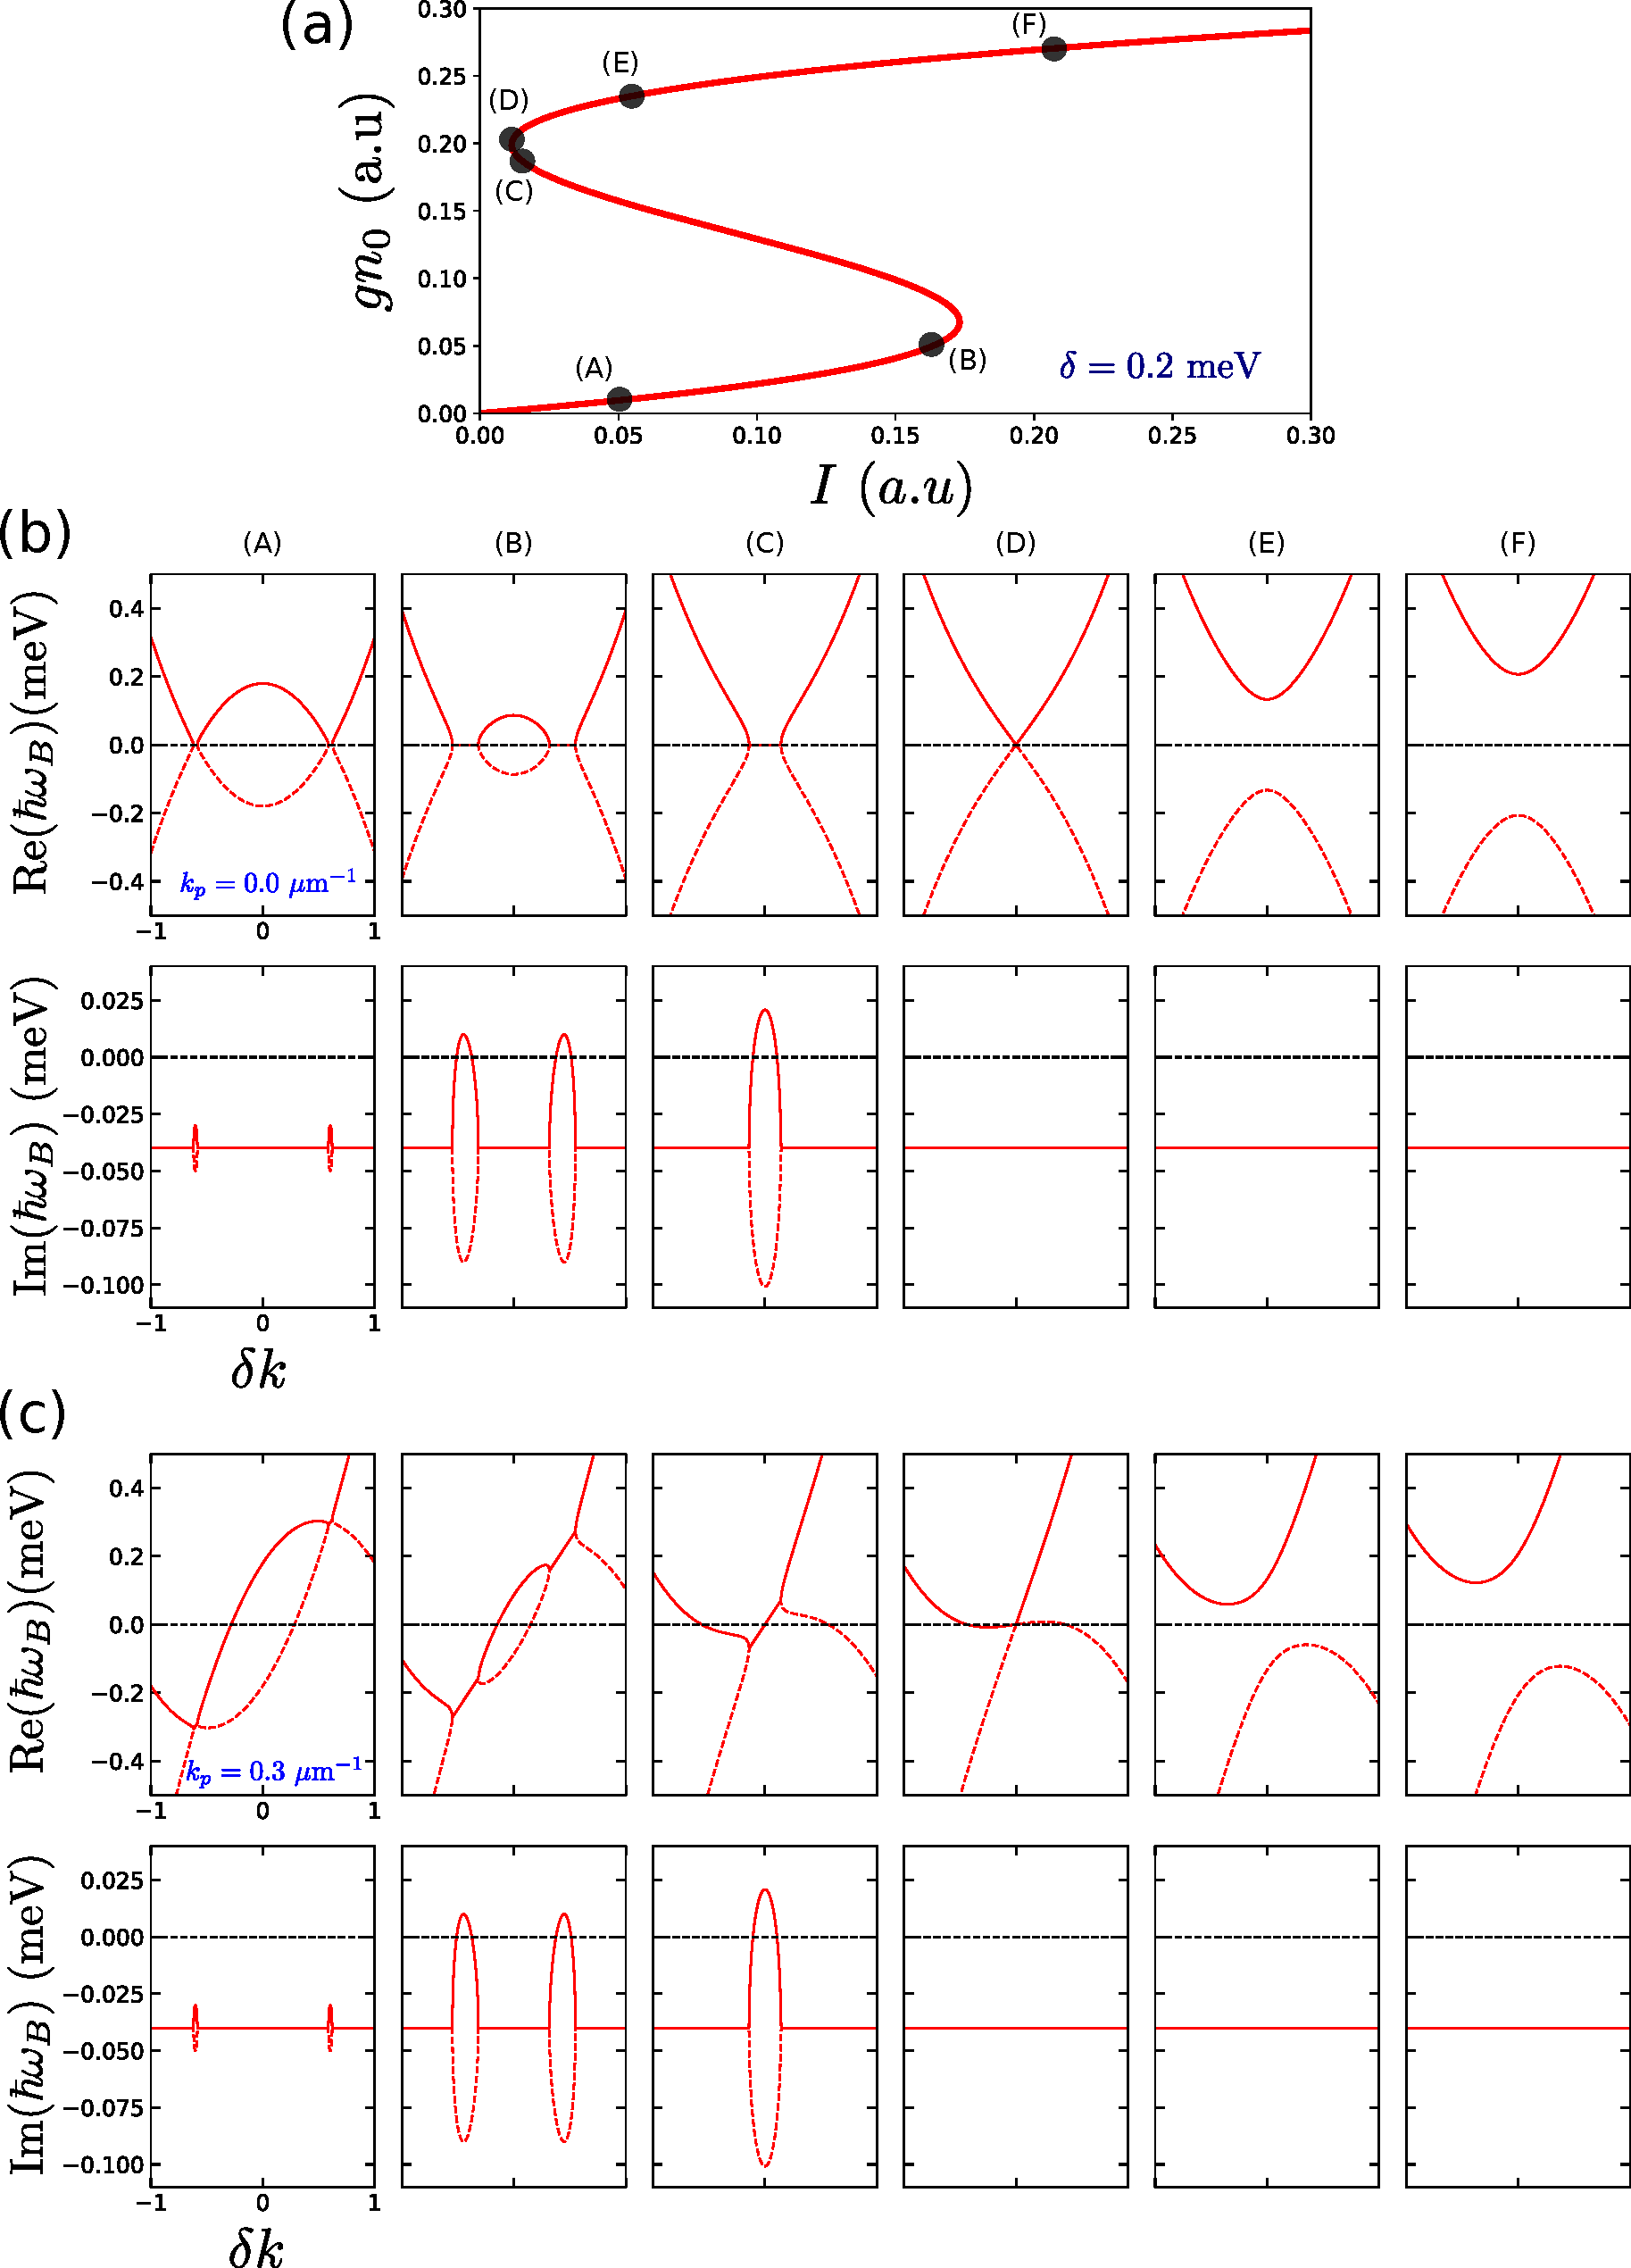
\includegraphics[width=1\textwidth]{chap_AG_theory/fig/bist_et_bogo.pdf}
   \label{fig:bist_et_bogo}
\end{figure}
\addtocounter{figure}{-1}
\begin{figure} 
    \caption{\textbf{Analytical Bogoliubov dispersion relations.} (a) Bistability curve of the fluid density $n_0$ as a function of the pump intensity $I$, calculated from \autoref{eq:steady_state}, for a pump detuning $\hbar\delta$ = 0.2 meV. (b) Positive (solid red lines) and negative (dashed red lines) solutions of the Bogoliubov dispersion relation in the fluid reference frame, computed from \autoref{eq:bogo_lab_frame}, at the pump wavevector $\kbf_p$ = 0 (zero flow velocity), at the pump detuning $\delta(0)$ = 0.2 meV and for pump intensities indicated by the points A, ..., F in (a). Upper line: real part of the energy of elementary excitations. The black dotted line highlights the pump energy. Lower line: imaginary part of the energy of the elementary excitations. As long as it remains negative (below the black dashed line), the Bogoliubov solutions are dynamically stable. Note that near and all along the negative slope branch of the bistability, the modes are unstable, giving rise at the point B and C respectively to modulation instabilities (coupling of the positive solution with the negative solution at $\kvec \neq 0$) and Kerr instabilities (coupling of the positive and the negative solutions with the pump mode at $\kvec = 0$). At the other points A, D, E, F, the system losses fix the imaginary part at $-\gamlp/2$, stabilizing the fluid. (c) Same considerations as for (b) but at a pump wavevector $k_p$ = 0.5 $\mu$m$^{-1}$. The fluid speed of flow is no longer zero, leading to an asymmetrization of the Bogoliubov solutions. In both (a) and (b) cases, the linearization of the solutions at low-k, relating the generation of phonon-type elementary excitations, appears only at the turning point D. \textit{Adapted from} \cite{claude_phd}}
    \label{analytical_bog}
\end{figure}

\bigskip 

\textbf{Linear spectrum.}
Let us first examine the most distinctive regime, which establishes a direct connection with conservative systems and was, in fact, the primary motivation for exploring this platform in the context of analog gravity experiments \cite{claude_high-resolution_2022}.
When the fluid operates at the turning point of the bistability (D) we demonstrated in the previous chapter that the detuning compensates the total interaction blueshift $\delta(0)=g_rn_r + gn_0$. 
Plugging this constraint in \autoref{eq:bogo_static} we obtain :

\begin{equation}
    \omega_B(k) = \pm \sqrt{\dfrac{\hbar k^2}{2\mlp} \left({\dfrac{\hbar k^2}{2\mlp}} + g n_0 \right)}.
\end{equation}

We introduce the healing length $\xi=\sqrt{\hbar^2/mgn_0}$ which is the characteristic length scale of the system below which the collective description of the fluid breaks down and microscopic effects
must be taken into account. The spectrum exhibits two trends depending whether $k$ is smaller or larger than $1/\xi$ as shown on the (D) plot of \autoref{fig:bist_et_bogo} \textbf{b)}. At low wavevector $k \ll 1/ \xi$ the spectrum is linear, for the normal branch we have :

\begin{equation}
    \re(\omega^+_B(k)) \sim c_s\abs{k}
\end{equation}
where $c_s = \sqrt{\hbar g n_0/\mlp}$ is the speed of sound in the fluid. For the ghost branch, represented by the red dashed line $c_s$ is be replaced by $-c_s$. At this operating point the driving laser is forcing the system exactly at its proper energy and 
doesn't fix the phase of the excitations. In this regime, the long range interactions are dominated by collective deformation of the fluid --phonons-- that propagate with the same group velocity $\partial\omega/\partial k =c_s$ regardless their wavevector. 
The idea of having --in the low wavevector limit -- a fixed velocity at all frequencies remind the light cone with the difference that the sound velocity is not the same in all the reference frames.
The linearity is a typical feature of quantum fluids and give rise to spectacular collective behavior such as superfluidity \cite{Amo_fluidlightexp_2009} as well as topological protection of quantized vortices and dark solitons \cite{maitre_thesis}.
The bogoliuvov spectrum was reported in several experiments \cite{utsunomiya_observation_2008,stepanov_dispersion_2019} with different experimental methods while the linearity have been measured with 
an unprecedented resolution in the group \cite{claude_high-resolution_2022}. The latter experiment was performed with a spectroscopy method recently developped \cite{claude_prb} that we will describe and use in the next chapter.

\bigskip

In the high wavevector limit, $k \gg 1/\xi $, we recover the standard parabolic dispersion blueshifted by the interaction.

\begin{equation}
    \re\left(\ombog^+(k)\right) \sim \dfrac{\hbar k^2}{2\mlp} + g n.
\end{equation}

It's worth noticing that at even higher wavevector the parabolic approximation is not true anymore and the full LP dispersion must be plugged in the bogoliubov matrix. In this case one would observe that the bogoliubov spectrum is flattened
by the exciton line at high wavevector \cite{I_frerot_PRX_2023}.

\bigskip

\textbf{Massive excitations regime.} If the system is brought further along the high density branch ie if $gn_0+g_rn_r>\delta(0)$ a gap opens in the spectrum and linearity is lost as it can be seen 
in plot (E) and (F). A limited development of the spectrum around $k=0$ gives the parabolic approximation:
\begin{equation}
    \re\left(\ombog^+(k)\right) \sim \omega^+_B(0) + \dfrac{\hbar k^2}{2\mlp}\dfrac{\left(2g n_0 + g_r n_r - \delta(0)\right)}{\sqrt{\left(2g n_0 + g_r n_r - \delta(0)\right)^2 - (g n_0)^2}}.
\end{equation}
This enable to provide the Bogoliubov modes with an effective mass :
\begin{equation}
    m_{\mathrm{det}}= \mlp\dfrac{\sqrt{\left(2g n_0 + g_r n_r - \delta(0)\right)^2 - (g n_0)^2}}{\left(2g n_0 + g_r n_r - \delta(0)\right)}.
\end{equation}
Note that in the limit $gn_0+g_rn_r\to \delta(0)$, the system recovers the massless scenario described earlier. 
The emergence of a gap in the spectrum can be understood as follows: when the system is driven too strongly relative to the turning point, the phase of the Bogoliubov excitations tends to become locked to the phase of the pump. 
This induces a form of "rigidity" in the fluid's phase, implying that introducing a phase fluctuation into the system requires a minimum energy.

\bigskip

In both of the previous regimes, the terms in the square root of \autoref{eq:bogo_static} remain positive at all wavevectors meaning the imaginary part of 
full dispersion never deviate from $\gamma/2$ as shown in the subpanels of \autoref{fig:bist_et_bogo} \textbf{b)} ensuring the stability of the system.

\bigskip

\textbf{Low density regime.} Conversely, when the sytem is operating on the lower branch of the hysteresis loop, the amount of interaction is not sufficient to 
compensates for the detuning. Equivalently, it means that for some value of the wavevector the term in the square root of \autoref{eq:bogo_static} becomes negative
giving rise to additionnal contribution to the imaginary part of the spectrum. Note that it doesn't necessarily mean that the system is unstable. Indeed, an instability 
requires that the overall imaginary part of $\omega^{\pm}_B$ is positive. At very low density like in (A), the inherent losses of the system 
are sufficient to dump the instability and the imaginary part remains negative at all $k$. If the pump strength is ramped up near the lower branch turning point (B) 
the imaginary part of the spectrum might become positive at some wavevector and make the system is unstable. Note that the point at which this happens depend on the experimental
parameters. Finally, the point (C), located between the two branches, has an imaginary part that is highly positive at low wavevectors. This is the reason why this branch of excitation
is often referred as unstable and can not be observed. 


\bigskip 

The discussion above also holds for the case of a moving fluid provided we set our description in the comoving frame and replace $k$ by $\delta k=k-k_p$ in \autoref{eq:bogo_static}.

\subsubsection{Moving polaritons at finite $k_p$}
In this section we consider again a fluid in motion at $\kbf_p\neq0$ that we describe in the lab frame. In terms of regime of collective excitations nature, the phenomenology is similar to the one
described above and the discussion can be carried out in the same way. The only difference is that the dispersion relation is now centered around the fluid wavevector $\kbf_p$ and "tilted" by the doppler effect. Consequently, the bogoliubov spectrum graphically 
loses an axis of symmetry which is a graphical manifestation that $\Lbog$ no longer respects the symmetry of \autoref{eq:symetry_bog}.
Again we set $\delta(k_p)=0.2 \mathrm{meV}$ and we plot the dispersion relation for the same operating points than in the static case, the results are presented in the subpanels of \autoref{fig:bist_et_bogo} \textbf{c)}. Note that the spectra are displayed as function 
of the wavevector in the fluid frame since \autoref{eq:bogo_lab_frame} mathematically depends only on $\delta k$ enabling to compare the spectra in the two reference frame.

\begin{figure}[!htbp]
    \centering
    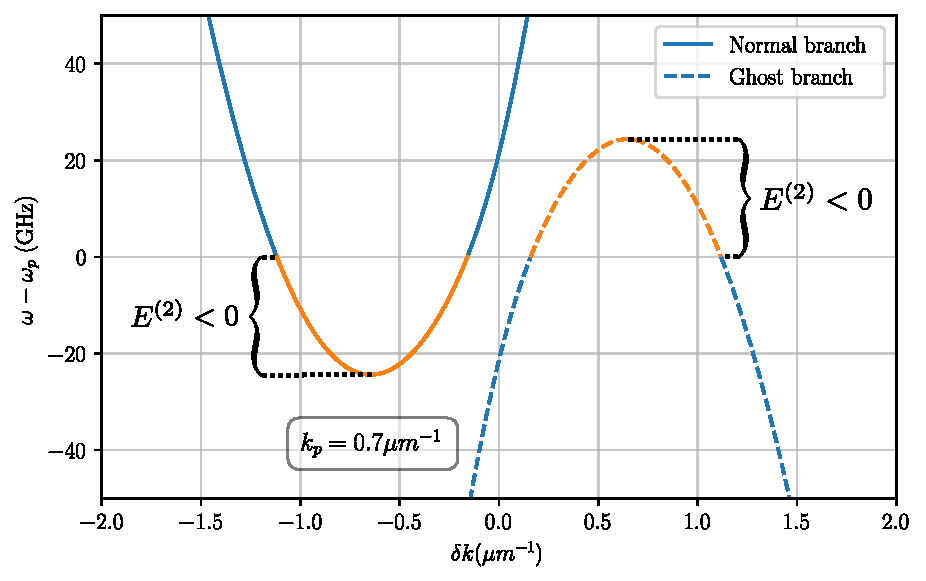
\includegraphics[width=\textwidth]{chap_AG_theory/fig/bogo_gap_supersonic_dispersion.pdf}
    \caption{Bogoliubov spectrum for a fluid in motion at $k_p=0.7 \mathrm{\mu m^{-1}}$ and $\delta(k_p)=0.2 \ \mathrm{meV}$. The dashed line represent the ghost branch ie the negative norm branch while the solid line
    represent the normal branch ie the positive norm branch. The blue color represents the positive energy modes while the orange represent the negative energy modes resulting from the 
    product of a norm and a frequency with opposite signs.}
    \label{fig:gapped_supersonic}
\end{figure}

In the linear case $gn_0+g_rn_r=\delta(k_p)$, the low wavevector slope is modified by the fluid velocity :
\begin{equation}
    \begin{aligned}
    \re\left(\ombog^+(\delta k)\right)& \sim (c_s + \vbf_0)\abs{\delta k} \ \ \mathrm{for} \ \delta k > 0 \\
    \re\left(\ombog^+(\delta k)\right)& \sim (c_s - \vbf_0)\abs{\delta k} \ \ \mathrm{for} \ \delta k < 0
    \end{aligned}
\end{equation}
From this, one can see that when the fluid is supersonic $\vbf_0>c_s$ as in plot (D) some modes of the normal branch --the positive norm modes-- are pulled down to the negative frequency domain. Symmetrically, some ghost branch modes --the negative norm modes-- are pulled up to the positive frequency domain.
In both case, the excitations carry negative energy as explained in \autoref{subsub:bogo_energy}, in this regime superfluidity is lost and any defect in the fluid flow 
can create excitations \cite{Amo_fluidlightexp_2009}. If the pump intensity is increased further like in (E) and (F), a gap opens again in the spectrum, the excitations are massive while
the negative energy modes may disappear due to the gap opening. However, it doesn't mean that the possibility to create excitations with negative energy 
is lost as soon as the spectrum is no longer linear. Indeed, increasing further the pump velocity can lead to situations where the spectrum is massive but still has negative energy modes.
A typical example of this case is presented in \autoref{fig:gapped_supersonic}, where the pump wavevector was set to $k_p=0.7 \mathrm{\mu m^{-1}}$ and the other parameters stayed the same. 
A gap is present but the doppler effect is strong enough to excite negative energy modes on both branches which are represented by the orange lines. Unlike the linear case, it is not possible to define 
a sound velocity for the low wavevector excitations. Consequently, the critical velocity to exceed for the apperance of negative energy modes doesn't match the velocity $\sqrt{\hbar g n_0/\mlp}$ that we still refer to as the sound velocity
by analogy with linear case. Moreover, since the velocity affects the dispersion itself through the detuning $\delta(k_p)$, the usual procedure of applying the Landau criterion---where the energy of excitations is modified solely through a Doppler shift $\omega_B(k) \to \omega_B'(k) + v_0 k$---is no longer valid. In this case, the spectrum itself is inherently altered by the fluid motion, meaning that the flow velocity does not simply act as a shift parameter but fundamentally changes the nature of the excitations.
 As a result, the criterion must be modified to account for this direct dependence. In practice, the knowledge of an analytical 
 expression for the critical velocity is not necessary and knowing that there exist one is sufficient as we will see in the experimental section.
 




\bigskip



It is now clear that depending on its velocity and parameters the fluid can exhibit a rich variety of collective excitations. Let us summarize what we reviewed  so far in this chapter.
\begin{tcolorbox}[infernoSummary]
    \begin{itemize}
        \item The polariton fluid exhibits a rich variety of collective excitations depending on the pump intensity and detuning through the bistability cycle. The different 
        modes are characterized by their norm and frequency.
        \item There exist a peculiar operating point at which the spectrum is linear allowing for the definition of a sound velocity $c_s=\sqrt{\hbar g n_0/\mlp}$.
        \item The spectrum can also be massive if the system is pumped further along the high density branch and the effective mass depend on the detuning and the pump intensity.
        \item In the low density regime, the spectrum can become unstable and exhibit a positive imaginary part. 
        \item Putting the fluid in motion can lead to the appereance of negative energy modes. The critical velocity for this to happen is a complex function of the detuning and the interactions. It doesn't 
         match the speed of sound $c_s$ as soon as the system doesn't operate at the turning point of the hysteresis loop.
    \end{itemize}
    \end{tcolorbox}


In particular, if we restrict ourselves to high density regime where, inherent losses appart, the bogoliubov dispersion remains real, the fluid can be either subcritical --all the modes carry positive energy-- or supercritical --some modes carry negative energy.
The long way we have made to proove that quite simple feature paves the way to already understand how Hawking radiation can be observed in a polariton fluid. Indeed, creating 
an interface between a subcritical and a supercitical region will mix positive and negative energy modes just as a gravitationnal event horizon would. Obviously, 
 showing that it can leads to paired correlated emission from vacuum will require to quantize the modes as we will see in the next section.

\section{Hawking radiation in a transcritical fluid}
 


\subsection{Inhomogeneous pumping}
We consider a driving pump defined as follow :

\begin{equation}
    F_p(r,t) = \left\{
        \begin{array}{ll}
            F_ue^{i(k_ux-\omega_p t)} & \mbox{if } \ x<x_h \\
            F_de^{i(k_dx-\omega_p t)} & \mbox{if} \ x>x_h
        \end{array}
    \right.
\end{equation}
where $x_h$ is an arbitrary position that will define the interface bewteen the two regions. The wavevectors are chosen so that $0<k_u<k_d$ and $k_d$ is sufficiently high to create a subcritical flow. The fluid is 
flowing toward the $x>0$ direction and the label $"u"$ and $"d"$ refer respectively to "upstream" and "downstream" region of the fluid with respect to the interface. We want to study Hawking emission of propagating modes so we set 
the laser frequency in order to ensure bistability in both region namely $\delta(k_u),\ \delta(k_d)>\sqrt{3}\gamlp/2$, and the pump amplitudes $F_u$ and $F_d$ so the fluids operate on the high density branch of their 
respective hysteresis cycle. Note that the pump is two dimensionnal but only depend on $x$. As we will justify it in the experimental section, the sample is in some extent also translationally invariant in the $y$ direction. Henceforth, we restrict our description to an effective 1D model.
Solving the GPE far from the interface gives two homogeneous regions with different asymptotic velocities $v_u=\hbar k_u/\mlp$ and $v_d=\hbar k_d/\mlp$, and different densities $n_u$ and $n_d$. We also 
account for fluctuations around each of these solutions the same way we did in the previous section which gives the asymptotic wavefunctions :

\begin{equation}
    \psi(x,t) = \left\{
        \begin{array}{ll}
            (\sqrt{n_u}+\dpsi_u)e^{i(k_ux-\omega_p t)} & \mbox{if } \ x \ll x_h \\
            (\sqrt{n_d}+\dpsi_d)e^{i(k_dx-\omega_p t)} & \mbox{if} \ x \gg x_h.
        \end{array}
    \right.
\end{equation}
\textcolor{red}{Note that continuity condition at $x_h$ makes the definition of the wavefunction near the interface unclear for now.}
Typical density and velocity profiles are shown in ??. For the sake of clarity, the speed of sound is plotted allowing direct comparison with 
the fluid velocity. We remind nonetheless that the previous section made clear that the relevant velocity to cross generally differ from $c_s$.

\bigskip

We wish to solve the scattering problem for the Bogoliubov modes at the interface. In each homogeneous region, fluctuations are plane wave oscilatting at $\omega$ of the form :
\begin{equation}
    \begin{pmatrix}
        u_k(x) \\
        v_k(x)
    \end{pmatrix} = \begin{pmatrix}
        U_k^u  \\
        V_k^u 
    \end{pmatrix}e^{i(k+k_{u,d})x}.
\end{equation}
The wavevector $k$ and frequency $\omega$ satisfy the Bogoliubov dispersion relation $\omega=\omega_B(k)$ that we remind here :

\begin{equation}
    \omega_B(k)=v_{u,d}k\pm\sqrt{\left(\dfrac{\hbar k^2}{2\mlp}-\delta(k_{u,d})+ g_rn_r +2g n_0\right)^2 - \left(g n_0\right)^2}-\dfrac{i\gamma}{2} 
    \label{eq:bogo_lab_frame_both_regions}
\end{equation}
where $v_{u,d}=\hbar k_u/\mlp$ are the fluid velocities in the upstream and downstream regions. The corresponding dispersions are plotted in \autoref{fig:bogo_up_and_down}. We see that, in the subcritical region ($x<x_h$), positive- and negative-norm modes are still found exclusively at positive and negative frequency, respectively.
However, in the supercritical region ($x>x_h$), some positive-norm modes are dragged to negative frequencies (and reciprocally for negative-norm modes) by the Doppler effect.

\bigskip


Since there is redundandy of the information with respect to the zero frequency line let us fix $\omega>0$ and look for the wavevectors $k$ satisfying $\omega=\omega_B(k)$ in each region.
\begin{figure}
    \centering
    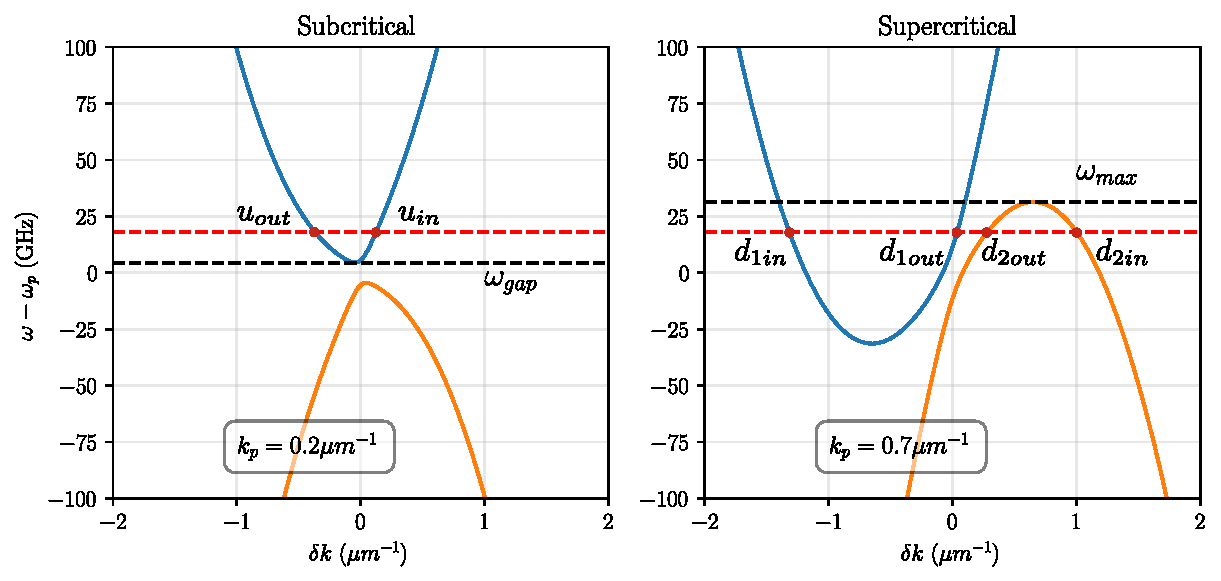
\includegraphics[width=1\textwidth]{chap_AG_theory/fig/bogo_gap_dispersion.pdf}
    \caption{\textbf{Bogoliubov spectrum in the upstream and downstream regions.} The Bogoliubov spectrum in the asymptotic upstream region \textbf{(a)} and downstream region \textbf{(b)} of the fluid, calculated from \autoref{eq:bogo_lab_frame} with $\delta(0)=30$ (GHz), $k_u= \SI{0.2}{\per \micro \meter}$ and
    $k_d=\SI{0.7}{\per\micro\meter}$.}
    \label{fig:bogo_up_and_down}
\end{figure}

\bigskip

\textbf{Subcritical region.} In the upstream region $x<xh$, for any $\omega>0$ there always exist two real solution corresponding to positive norm modes as visible on the left panel of \autoref{fig:bogo_up_and_down}. Depending
on the sign of their group velocity $v_g=\partial\omega/\partial k$, we label the solution $"out"$ if it propagates away from the interface and $"in"$ if it goes toward the interface. 
Taking the square of \autoref{eq:bogo_lab_frame_both_regions} the problem can be cast under a real coefficient polynomial equation of degree 4 in $k$. As a consequence,
there exist two additionnal complex conjugate solutions. Depending on the sign of their imaginary part, they are either exponentially growing or decaying. 

\bigskip


\textbf{Supercritical region.} In the downstream region $x>x_h$, the situation is different and require a disjunct analysis. If $\omega>\omega_{max}$ the situation is the same than in the upstream 
region. There exist two propagating solutions $d_{1in}$ and $d_{1out}$ lying on the normal branch with opposite group velocity as well as two non propagating modes. When $\omega<\omega_{max}$, in addition to the positive norm solution, the doppler shift pull two negative norm solutions $d_{2in}$ and $d_{2out}$ herited from $\omega=\omega^-_B(k)$


\textbf{Scattering solutions-\textit{in} global modes}
A general function to describe the fluctuations at $\omega$ is obtained by the linear combination of all the possible propagating solutions :
\begin{equation}
    \begin{pmatrix}
        u_k(x) \\
        v_k(x)
    \end{pmatrix}_{u,d} = \left(\sum_{i\in \mathrm{in}}\betin_i e^{ik^{in}_ix}\begin{pmatrix}
        U_{k^\mathrm{in}_i}  \\
        V_{k^\mathrm{in}_i}
    \end{pmatrix}+\sum_{i\in \mathrm{out}}\betout_i e^{ik^{out}_ix}\begin{pmatrix}
        U_{k^\mathrm{out}_i}  \\
        V_{k^\mathrm{out}_i}
    \end{pmatrix}\right)_{u,d}
\end{equation}
From this expression we can form the so called scattering solutions. Such a solution reflect how a given mode impinging on the interface is scattered into the other channels.
For instance, for the case of an incoming mode from the upstream region, the scattering solution is a piece-wise function given by :
\begin{itemize}
    
\item\begin{equation}
    \begin{pmatrix}
        u_k(x) \\
        v_k(x)
    \end{pmatrix}_{u} =\betin_ue^{{ik_u^{{\mathrm{in}}x}}}\begin{pmatrix}
        U_{k^\mathrm{in}_{u}} \\
        V_{k^\mathrm{in}_{u}}
    \end{pmatrix}
    +
    \betout_u e^{ik_u^{{\mathrm{out}}x}}\begin{pmatrix}
        U_{k^\mathrm{out}_{u}} \\
        V_{k^\mathrm{out}_{u}}
    \end{pmatrix} \ \mathrm{for} \ x\leq x_h
\end{equation}  

\item\begin{equation}
    \begin{pmatrix}
        u_k(x) \\
        v_k(x)
    \end{pmatrix}_{d} = \betout_{d2} e^{ik^{\mathrm{out}}_{d2}x}
    \begin{pmatrix}
        U_{k^\mathrm{out}_{d2}} \\
        V_{k^\mathrm{out}_{d2}}
    \end{pmatrix} + \betout_{d1} e^{ik^{\mathrm{out}}_{d1}x}
    \begin{pmatrix}
        U_{k^\mathrm{out}_{d1}} \\
        V_{k^\mathrm{out}_{d1}} 
    \end{pmatrix} \ \mathrm{for} \ x\geq x_h.
\end{equation}
\end{itemize}

A given solution and its derivative has to be a continuous in space which imposes matching condition at the interface. This condition will fix the coefficients $\beta_i^{in}$ and $\beta_i^{out}$ that can be interpted as reflection and transmission coefficents of the incoming wave at the inteface. 
These modes are definded on the whole space and solve the equations of motion everywhere. From the three $in$ modes $u_{in}$ $d_{1in}$ and $d_{2in}$ in the $\omega_{gap}<\omega<\omega_{max}$ regime it is possible to construct three scattering solutions. At a given frequency $\omega$ one can verify that these solutions are orthonormal with respect to the Bogoliubov inner product :
\begin{equation}
    \bra{\dpsi^\mathrm{in}_i(\omega)}\ket{\dpsi^\mathrm{in}_j(\omega')}_B = \int \mathrm{d}x  \ u^*_{i,\omega}(x)u_{j,\omega'}(x)-v^*_{i,\omega}(x)v_{j,\omega'}(x)  = \mathrm{sign}(\bra{\psi^\mathrm{in}_i}\ket{\psi^\mathrm{in}_i}_B)\delta_{ij}\delta(\omega-\omega').
\end{equation} 
where $i,j \in \{u_{in},d_{1in},d_{2in}\}$ and $\mathrm{sign}$ is the sign function. 
As defined, the $in$ global modes (GM) form a basis of the Bogoliubov problem valid at any $x$ in the system.

\bigskip

\textbf{Outgoing global modes.} It also possible to define the global solution of an outgoing wave. Take the outgoing mode $d_{1out}$ in the downstream region, in the scattering picture it results from the 
 the transmission of an ingoing upstream mode $u_{in}$ and the reflection of the two ingoing downstream modes $d_{2in}$ and $d_{1in}$. Doing this procedure in the $\omega_{gap}<\omega<\omega_{max}$ range, the three $out$ modes
define three outgoing GM. Just as the $in$ solutions, the $out$ ones form an orthonormal basis of the solution space.

Since we found two basis describing the same set it is possible to express the $out$ modes in terms of the $in$ modes. 
Each three $out$ modes are linear combination of the three $in$ modes which define the so called $3\times3$ scattering matrix $S(\omega)$ :

\begin{equation}
    \begin{pmatrix}
        \betout_{u}(\omega) \\
        \betout_{d1}(\omega) \\
        \betout_{d2}(\omega)
        \end{pmatrix} =
    S(\omega)\begin{pmatrix}
        \betin_{u}(\omega) \\
        \betin_{d1}(\omega) \\
        \betin_{d2}(\omega)
    \end{pmatrix}.
    \label{eq:scattering_matrix}
\end{equation}
Note that in $\omega>\omega_{max}$ case the $d_{2out}$ mode is not present and the scattering matrix should be $2\times2$. However, to keep 
the notation the same everywhere, we also take into account the evanescent modes and allow coefficient some coefficient to be zero in the scattering matrix.

Since the orthonormal structure of the Bogoliubov modes was built with the modified norm $\bra{\cdot}\ket{\cdot}_B$ it imply
that $S$ is unitary for the corresponding extented metric $\nu$ :

\begin{equation}
    S^\dagger(\omega)\eta S(\omega) = \eta.
    \label{eq:unitarity}
\end{equation}
where $\nu=\mathrm{diag}(1,1,-1)$. The unitary condition ensure energy conservation even in the presence of negative energy modes.  Indeed, the $-1$ sign in the third diagonal term account for norm conversion and originate from the scattering of positive norm modes into negative norm modes.
The square modulus of a given coefficient $\abs{S_{ij}}^2$ gives the proability of reflexion or transmission of the mode $i$ into the mode $j$.

To make this point clear, let us tackle the example of the scattering of an incoming mode $u_{in}$ with energy $\hbar\omega$ in the upstream region. 
There is a probability $\abs{S_{uu}}^2$ that the mode get reflected in $u_{out}$ and a probability $\abs{S_{d1u}}^2$ that it gets transmitted into $d_{1out}$ both of this mode have the same energy. The remaining term $\abs{S_{u2}}^2$ is the probability that the mode get transmitted into a negative norm mode $d_{2out}$ which has the opposite energy $-\hbar\omega$
The unitary condition \autoref{eq:unitarity} ensures that the total energy is conserved $1=\abs{S_{uu}}^2+\abs{S_{d1u}}^2-\abs{S_{d2u}}^2$.


It is interesting to stress that the asymptotic classification of modes as $in$ or $out$ mirrors the procedure used in the study of quantum fields in black hole spacetimes, where a causal, time-oriented interpretation is adopted: in modes represent incoming configurations in the remote past, while out modes correspond to outgoing configurations in the distant future.
 This structure forms the basis of the Bogoliubov transformation formalism, which relates the two mode bases and captures the mixing between positive and negative frequency components that underlies processes such as particle production.
\subsection{Modes quantization}
\label{subsec:quantization}
So far, we described the fluctuations of the order parameter as classical fields. This approach
show that the bogoliubov modes can exist in the system as solutions to the equations of motion. The scattering matrix
a priori tells us how an incoming wavepacket is scattered at the interface.
Yet, our classical description require an external pertubation to inject non zero amplitude in a given mode. Hence it doesn't
predict what would happen with highly non classical state as an input, like the vacuum state. To achive this, we need to quantize the modes.

\textbf{Quadratic Hamiltonian.} The first step is to write the field operator : 
\begin{equation}
    \hat{\psi}(x,t)= \psi_0(x,t)\hat{a}_{\psi_0}+\hat{\dpsi}(x)
\end{equation}
where $\hat{a}_{\psi_0}$ is the operator that annihiliate a polariton in the mean field state and $\hat{\dpsi}(x)$ is the fluctuation operator that 
annihilate a fluctuation. Pluggin this ansatz into the GPE in its second quantization form \ref{eq:pol_non_linear_hamiltonian} and going to first order in the fluctuations, one
finds that the hamiltonian has a quadratic form in the fluctuation operator. As a consequence, the Heisenberg
equations of motion for the Bogoliubov operator are linear in the fluctuations \cite{castin_bose-einstein_2001}. This property is of great importance.
Indeed, it allows to use a very simple quantization procedure. The fully quantum decomposition of the 
fluctuation operator is obtained from its classical counterpart ~\ref{eq:general_solution_for_fluctuations_classical} by promoting the coefficients $b_k$ to bosonic operators. A positive norm modes coefficient
is promoted to an annihilation operator $\bk$ while a negative norm mode has to be replaced by a creation operator. Under this prescription
the classical fluctuations field becomes :

\begin{equation}
    \delta\hat{\psi}(x,t) =\sum_{k\in S_+}\left[u_k(x)\bk e^{-i\omega_k t}+ v^*_k(x)\bkdag e^{i\omega_k t}\right]
\end{equation}
with the commutation relation 
\begin{equation}
    \norm{\phi_i}_B\norm{\phi_j}_B[\hat{b}_i, \hat{b}_j^\dagger]  = \norm{\phi_i}_B\delta_{ij}
\end{equation}
which is the usual bosonic commutation relation for positive norm modes while for negative norm modes the annihilation operator and the creation operator are exchanged. To encode this property in a convenient way in the notation we rewrite the fluctuation field in a way that also count modes with negative 
norm at the cost of a redundancy.

\begin{equation}
    \delta\hat{\psi}(x,t) =\sum_{k\in S_+}\left[u_k(x)\bk e^{-i\omega_k t}+ v^*_k(x)\bkdag e^{i\omega_k t}\right] + \sum_{k\in S_-}\left[u_k(x)\bkdag e^{-i\omega_k t}+ v^*_k(x)\bk e^{i\omega_k t}\right]
    \label{eq:fluctuation_field_local_modes}
\end{equation}
This writting has the advantage of making explicit that for negative norm modes the frequency $\omega_k$ is associated to annihilation operators reflecting the particle-hole symmetry :
the creation of a particle a yields the same contribution as the annihilation of a hole.



This procedure remains valid regardless the basis initially chosen and can especially be applied to the global modes exhibited earlier. The fully quantized fluctuations field for fluctuations can then be expressed in terms of $in$ global operators as :

\begin{equation}
    \hat{\dpsi}(x,t) = \int \mathrm{d}\omega\sum_{j\in \{u_{in},d_{1in}\} }[\ha_j(\omega)u_{j,\omega}(x)+\hadag_j(\omega)v^*_{j,\omega}(x)] + \int \mathrm{d}\omega[\hadag_{d_2}(\omega)u_{d_2,\omega}(x)+\ha_{d_2}(\omega)v^*_{d_2,\omega}(x)]
    \label{eq:fluctuation_quantization}
\end{equation}
where the operator $\hat{a}_j(\omega)$ is the operator that annihilates a global $in$ mode in channel $j$ at frequency $\omega$. An equivalent
expression can be written for the $out$ global modes noted $\hb_i$. The two sets of operators are again related by the scattering matrix :

\begin{equation}
    \begin{pmatrix}
        \hat{b}_u(\omega) \\
        \hat{b}_{d1}(\omega) \\
        \hat{b}_{d2}^\dagger(\omega)
    \end{pmatrix}=S(\omega)\begin{pmatrix}
        \hat{a}_u(\omega) \\
        \hat{a}_{d1}(\omega) \\
        \hat{a}_{d2}^\dagger(\omega)    
    \end{pmatrix}
\end{equation}


Few comments are in order at this stage. First, since we deal with quadratic Hamiltonian, the matrix is exactly the same obtained in the classical case.
From an experimental point of view this property is a crucial asset. Indeed, it means one can reconstruct the full matrix and hence all its quantum 
properties by just solving the scattering problem for classical modes which are much easier to engineer than quantum state. Any quantum correlation between the modes are in fact encoded in the matrix coefficient 
under phase and amplitude value of the reflexion-transmission coefficients. Of course, solving the scattering problem
would only be a way to infer correlations between the modes but not to measure them. Still, it gives information about what you can expect from a given 
analog horizon.

\bigskip

Secondly, while the $in$ and $out$ operators describe the same physical system they generate two different Fock states and thus two distinct vacuum states $\ket{0_{\mathrm{in}}}$ and $\ket{0_{\mathrm{out}}}$, as explained in the harmonic oscillator example.
This raises the question of whether a preferential basis can be found to provide a unequivocal description of the system: it is not the case.
 Indeed, unlike the Harmonic oscillator the system doesn't exhibit symmetries that justify one choice over the other. This being said, the $in$
and $out$ basis remain wise choices to describe the system since they are natural basis to infer what can be measured in the lab.

\bigskip

Finally, the transformation induced by the scattering matrix between the $in$ and $out$ operators is a Bogoliubov transformation where the 
normalisation condition is contained in the unitarity condition \ref{eq:unitarity}. We already discussed how such a transformation is the heart 
of any particle creation process and in particular of the gravitational Hawking radiation.  
WWhile very different,  these two systems  have in common the presence of a horizon that mixes positive and negative energy modes. The polariton platform is then an interesting system to study quantum field theory predictions --initially made for gravitational event horizons-- through the universality of the underlying 
mathematical structure, a Bogoliubov transformation.

\subsection{Spontaneous emission}

\label{subsec:spontaneous_emission}

Now that we have a fully quantized description of the system, expectation values of physical observables can be straightfrowardly
computed by plugging the desired input quantum state and look how it is modified by the scattering matrix. Let us start with the most spectacular and that
Stephen Hawking demonstrated in its original work \cite{hawking_black_1972} : spontaneous emission of correlated pairs from vacuum.


We are interested in the expectation value of the outgoing mode that is radiated by the interface away from the supercritical region $\hat{b}_u$.
Its decomposition in terms of the $in$ modes is :

\begin{equation}
    \hat{b}_u = S_{uu}\hat{a}_u + S_{ud_1}\hat{a}_{d_1} + S_{ud_2}\hat{a}_{d_2}^\dagger.
\end{equation}
The corresponding number operator $\hat{N}_u^{out}=\hat{b}_u^\dagger\hat{b}_u$ then reads :
\begin{equation}
    \begin{aligned}
        \hat{N}_u^{out} = &\abs{S_{uu}}^2\hat{a}_u^\dagger\hat{a}_u + \abs{S_{ud_1}}^2\hat{a}_{d_1}^\dagger\hat{a}_{d_1} + \abs{S_{ud_2}}^2\hat{a}_{d_2}\hat{a}_{d_2}^\dagger \\ 
        + & S_{uu}^*S_{ud_1}\hat{a}_u^\dagger\hat{a}_{d_1}+ S_{uu}^*S_{ud_2}\hat{a}_u^\dagger\hat{a}_{d_2}^\dagger + S_{ud_1}^*S_{uu}\hat{a}_u^\dagger\hat{a}_{d_1}^\dagger  \\
        + & S_{ud_1}^*S_{ud_2}\hat{a}_{d_1}^\dagger\hat{a}_{d_2}^\dagger+ S_{ud_2}^*S_{uu}\hat{a}_{d_2}\hat{a}_u+ S_{ud_2}^*S_{ud_1}\hat{a}_{d_2}\hat{a}_{d_1}. 
    \end{aligned}
\end{equation}
Using the bosonic commutation relation for the negative norm term $\abs{S_{ud_2}}^2\hat{a}_{d_2}\hat{a}_{d_2}^\dagger=\abs{S_{ud_2}}^2(1+\hat{a}_{d_2}^\dagger\hat{a}_{d_2})$, the expectation
value of the number operator in the $in$ vacuum state $\ket{0_{in}}$ is :

\begin{equation}
    \bra{0_{in}}\hat{N}_u^{out}\ket{0_{in}} = \abs{S_{ud_2}}^2 
\end{equation}
In the $\omega \notin [\omega_{gap}, \omega_{max}]$ frequency range, the $d_2$ mode is not present and there is no emisssion. Conversely, when $\omega_{gap}<\omega<\omega_{max}$ 
the negative energy mode $d_2$ is present and yields a non zero emission from vacuum. This is the so-called Hawking effect. In fact,
 this radiation is correlated with all the other outgoing modes and one could even show tripartite entanglement among them \cite{isoard_quantum_2019}. Nonetheless, this is beyond the
 scope of this work and we will not go into the details of this calculation. Usually in the litterature, correlation at the horizon 
 between the out mode are inferred by computing the two point density correlation function \cite{Recati_acousticHR_2009, nguyen_acoustic_2015} :

 \begin{equation}
    g^{(2)}(x,x')=\dfrac{\langle{\hat{\dpsi}}^\dagger(x)\hat{\dpsi}^\dagger(x')\hat{\dpsi}(x)\hat{\dpsi}(x')\rangle}{\langle \hat{\dpsi}^\dagger(x)\hat{\dpsi}(x)\rangle\langle \hat{\dpsi}^\dagger(x')\hat{\dpsi}(x')\rangle}
 \end{equation}
 Plenty of numerical study in the group have been performed \cite{jacquet_quantum_2023}, and demonstrated that the interface of transcritical 
 flow of polariton can indeed exhibits Hawking radiation signature in its density correlation map.


 An experimental measurement of this correlation map has already been performed in Bose Einstein Condensate of Rb atoms \cite{steinhauer_observation_2016}.
 In this experiment the same analogue black hole is created 7400 times, each shot provide a realization of the density fluctuation map. The two point density correlation
 function is then computed by taking the average of $\hat{\dpsi}^\dagger(x)\hat{\dpsi}^\dagger(x')\hat{\dpsi}(x)\hat{\dpsi}(x')$. 
 In the case of a polariton fluid the density fluctuations map is harder to obtain due to 
 the out of equilibrium nature of the system. Indeed, due to the finite lifetime of the polaritons $1/\gamma\sim \SI{10}{\pico \second}$, a single 
 image of the fluid, even with the fastest camera, is already the results of many realization of the fluctuations which hence average to zero. In the conservative case,
 a given shot of the experiment freezes the system at given time when the trap is released. Therefore, looking for spontaneous
 emission in the polariton fluid is not a trivial task. As a first approach one can look for a stimulated version of the experiment which, in the light of the previous section,
 can be theoretically grasped by injecting a coherent state in the scattering problem.
 \textcolor{red}{pas sur de ce que je raconte ici}

\subsection{Stimulated emission}

Consider a coherent state input state $\ket{\alpha_{in}}$ in the upstream region eigenstate of the annihilation operator $\hat{a}_u$ with eigenvalue $\alpha_u \in \mathbb{C}$.
By just using that $\hat{a}_u\ket{\alpha_{in}}=\alpha_u\ket{\alpha_{in}}$ the expectation value in this state is straightfrowardly computed as :
\begin{equation}
    \bra{\alpha_{in}}\hat{N}_u^{out}\ket{\alpha_{in}} = \abs{S_{uu}}^2\abs{\alpha_u}^2 + \abs{S_{ud_2}}^2\abs{\alpha_u}^2
    \label{eq:stimulated_expectation_value}
\end{equation}
The presence of a coherent input state give rise to an additionnal term $\abs{S_{uu}}^2\abs{\alpha_u}^2$ which is the "classical" reflexion of the input mode on the interface.
To obtain a full scattering picture we also compute what is transferred in the other outgoig modes. The calculation are similar and we find :

\begin{equation}
    \bra{\alpha_{in}}\hat{N}_{d_1}^{out}\ket{\alpha_{in}} = \abs{S_{d_1u}}^2\abs{\alpha_u}^2 + \abs{S_{d_1d_2}}^2
    \label{eq:d1_stimulated_expectation_value}
\end{equation}
for the $d_1$ outgoing mode and 
\begin{equation}
    \bra{\alpha_{in}}\hat{N}_{d_2}^{out}\ket{\alpha_{in}} = \abs{S_{d_2u}}^2\abs{\alpha_u}^2 + \abs{S_{d_2d_2}}^2
    \label{eq:d2_stimulated_expectation_value}
\end{equation}
for the $d_2$ outgoing mode. This negative energy mode can be interpreted as the Hawking partner of the positive energy mode $u_{out}$ studied in the first place.
If we assume that $\abs{\alpha_u}$ is large enough, the first term in each of the above equation dominates the second one which gives :

\begin{equation}
    \dfrac{\bra{\alpha_{in}}\hat{N}_i^{out}\ket{\alpha_{in}}}{\abs{\alpha_u}^2} \approx \abs{S_{i u}}^2 \ \mathrm{for} \ i\in\{u,d_1,d_2\}.
\end{equation}
This quantity is accessible in the lab since it boils down to measuring the classical reflexion and transmission coefficients of the interface when a
coherent state is sent toward the interface from the upstream region. Eventhough this feature is not triggered by quantum vacuum 
fluctuations it is still a manifestation of the Hawking effect. To understand this one must compare the scenarios
whether $\omega$ is in $[\omega_{gap}, \omega_{max}]$ or not. In the latter case, energy conservation is simply $\abs{S_{uu}}^2\abs{\alpha_u}^2+\abs{S_{d_1u}}\abs{\alpha_u}^2=\abs{\alpha_u}^2$ and reflects that each of the output channels
carry a fraction of the incoming energy. While when $\omega \in [\omega_{gap}, \omega_{max}]$ the same condition reads $\abs{S_{uu}}^2\abs{\alpha_u}^2+\abs{S_{d_1u}}^2\abs{\alpha_u}^2-\abs{S_{d_2u}}^2\abs{\alpha_u}^2=\abs{\alpha_u}^2$ due to the negative energy mode.
This directly implies $\abs{S_{uu}}^2\abs{\alpha_u}^2+\abs{S_{d_1u}}^2\abs{\alpha_u}^2\geq \abs{\alpha_u}^2$ which means that the two positive energy channels
carry more energy than what was injected, the excess being compensated by the negative energy mode. This amplification means that the incoming 
coherent state extracted energy from the transcritical region by exciting a negative energy mode.This is the same 
argument that led to the prediction of rotationnal superradiance in black hole physics \cite{hawking_black_1972} as well as in classical electromagnetic systems \cite{zeldovich__1970}.

\section{Conclusion}

In this chapter, we have explored the theoretical framework underlying the observation of Hawking radiation in a polariton quantum fluid. Starting from the Gross-Pitaevskii equation, we derived the Bogoliubov spectrum of collective excitations, highlighting the rich variety of regimes depending on the fluid's density, velocity, and interaction strength. We demonstrated how the interplay between positive- and negative-energy modes leads to the possibility of particle creation at a transcritical interface, analogous to the Hawking effect in black hole physics.

The quantization of Bogoliubov modes revealed the fundamental role of the scattering matrix in describing the mixing of positive- and negative-norm modes at the horizon. This mixing not only enables spontaneous emission from vacuum but also provides a framework to study stimulated emission, where coherent input states amplify the Hawking-like radiation. Importantly, we showed that the amplification of outgoing modes is driven by the presence of negative-energy modes.

These results establish a theoretical foundation for the experimental investigation of analog Hawking radiation in polariton systems. By leveraging the properties of polariton fluids, such as their out-of-equilibrium nature and tunable parameters, this platform offers a promising avenue to probe fundamental aspects of quantum field theory in curved spacetime. In the next chapter, we will focus on the experimental implementation of these concepts and the challenges associated with observing Hawking radiation in practice.
% !TeX encoding = UTF-8
% !TeX spellcheck = fr_FR
% !TeX root = ../mythesis.tex
% !TeX program = pdflatex (build)
%%% TeXmaker : no 'magic comments' but set Root with Options > Set as master file

%useful stuff for what follows

\newcommand{\kbf}{\pmb{k}}
\newcommand{\vbf}{\pmb{v}}
\newcommand{\rbf}{\pmb{r}}
\newcommand{\ombog}{\omega_{\mathrm{b}}}

\newcommand{\rmexp}{\mathrm{exp}}
\newcommand{\im}{\mathfrak{Im}}
\newcommand{\re}{\mathfrak{Re}}
\newcommand{\mbogo}{m_{\mathrm{det}}}
\newcommand{\cs}{c_{\mathrm{s}}}
\graphicspath{{./}{./fig/}{./chap_custom_st/fig/}}

\chapter{Optical generation and spectroscopy of arbitrary acoustic horizons}

\label{chap:generation_transonic_fluid}

The study of particle creation in the presence of highly curved spacetime has been a subject of interest for many years. The most famous example is the Hawking radiation \cite{hawking_black_1972}, which predicts the creation of particles from the vacuum in the vicinity of a black hole event horizon enabling the black hole 
to evaporate. The obvious difficulty to test this prediction experimentally is double. First, the blackness of such an object makes it hard to spot with a telescope meaning one have to rely rather on the peculiar behavior of visible object moving in the gravitationnal field of such a supermassive object. The optical observation of a black hole took almost one century since the first prediction of gravitationnal collapse by Subrahmanyan Chandrasekhar in 1920. It required 
the synchonization of nine telescope across the world to obtain an optical system whose optical aperture is the size the diameter of earth. the black body temperature of 

As mentionned in the previous chapter, the creation of a sonic horizon in a polariton fluid can lead to spontaneous emission of bogoliubov modes provided the downstream region collective excitation spectrum
exhibits negative energy modes. Furthermore, it was shown that the strength of the emitted signal depends strongly on the curvature of the horizon, or in other words, its steepness. To ensure that such effect is in principle observable in the lab, one need to fully characterize the mean field of the fluid as well as locally probe its excitation spectrum. This chapter is dedicated to the description of the fully optical generation of arbitrary transonic fluids as well as the characterization of the excitation spectrum on both side of the horizon. 
The latter revealed the first measurement of negative energy modes in a supersonic quantum fluid, validating the possibility to observe particle creation in a polariton fluid.

The first part will focus on the generation of mean fields with arbitrary velocity profile through the shapping of the pump laser phase. In a second part, we will present the pump probe spectroscopy method used to locally measure the collective excitation spectrum as well
as the results obtained on several transonic fluids. The results obtained are reported in Ref ??

\section{Optical generation of arbitrary fluid velocity field}


Let us set the coordinates $x$ and $y$ to describe the microcavity plane. As explained in Chapter 2, translationnal invariance in the $xy$-plane ensure in plane momentum conservation along photon absorption, while the wavevectors along the
$z$ direction are fixed by the cavity and quantum well lengths. Furthermore, in this experiment the laser beam is set to be quasi resonant with the lower polariton branch. As a consequence, the transverse phase of the laser is directly imprinted on the polariton field.
Indeed, in the low wavevector limit, the lower polariton branch can be safely approximated by a parabola, namely :

\begin{equation}
    \omega_{LP}(\kbf) = \omega_{LP}^0 + \dfrac{\hbar k^2}{2m_{LP}}.
\end{equation}

The group velocity of a polariton is then $\vbf = \frac{\partial \omega_{LP}}{\partial k} = \frac{\hbar \kbf}{m_{LP}}= \frac{\hbar \kbf_p}{m_{LP}}$ where $\kp$ is the in-plane wavector of the pump laser.
In the case of a plane wave $\kp=\vec{\nabla}\theta(\rbf)$ where $\theta(r)$ is the spatial phase. This can safely be generalized to more complex spatial phase profile,
which provide a direct link between the driving laser phase and the velocity of the fluid :

\begin{equation}
    \vbf = \dfrac{\hbar \vec{\nabla} \theta(\rbf)}{m_{LP}} .
\end{equation}

\subsection{Waterfall configuration}

A first realisation of a 1D acoustic black hole in a polaritonic system was done in \cite{nguyen_acoustic_2015} with the so called waterfall configuration. 
The setup was composed of a microcavity etched to be truly one dimensionnal and a defect was added in the middle of the wire to act as an external attractive potential and force the polariton flow to accelerate. The pump was only shone in the region before the defect. The downstream region of the flow was then made of polariton that propagate balistically and whose speed is fixed by the interaction energy
in the upstream region.
Eventhough this configuration provide a natural fluid acceleration, the horizon geometry depends greatly on the defect shape and can not be tuned easily.  Furthermore, the collective excitation spectrum and the presence of negative energy modes was not investigated which 
prevent to conclude on the nature of the signal observed in the experiment. In the present work, we present a different approach to generate such flows with an effective 1D fluid fully optically created as well as a full characterization of the Bogoilubov spectrum.

\subsection{Target velocity profile}
Before analyzing whether the fluid surpasses a critical velocity, the primary objective is to generate a flow exhibiting two homogeneous regions separated by a sharp transition, each characterized by a well-defined velocity. For clarity, the region preceding the transition will be referred to as the upstream region, with velocity $v_{up}$ while the region following the transition will be designated as the downstream region, with velocity $v_{d}$.
To model this configuration, a target velocity profile is arbitrarily defined as follows:"
\begin{equation}
    v(x)= \frac{v_{d}-v_{up}}{2}\mathrm{tanh}(\frac{x-x_h}{w_h})+\frac{v_{up}+v_{d}}{2}
    \label{eq:target_velocity}
\end{equation}
where $x_h$ and $w_h$ are the position and width of the transition respectively. This profile is represented in \autoref{fig:target_velocity.pdf} a).
One can then verify that :

\begin{subequations}
    \begin{align}
    &\lim\limits_{x-x_h\ll-w_h} v(x) = v_{up},\\
    &\lim\limits_{x-x_h\gg+w_h} v(x) = v_{d}.
    \end{align}
\end{subequations}

\begin{figure}[h]
    \centering
    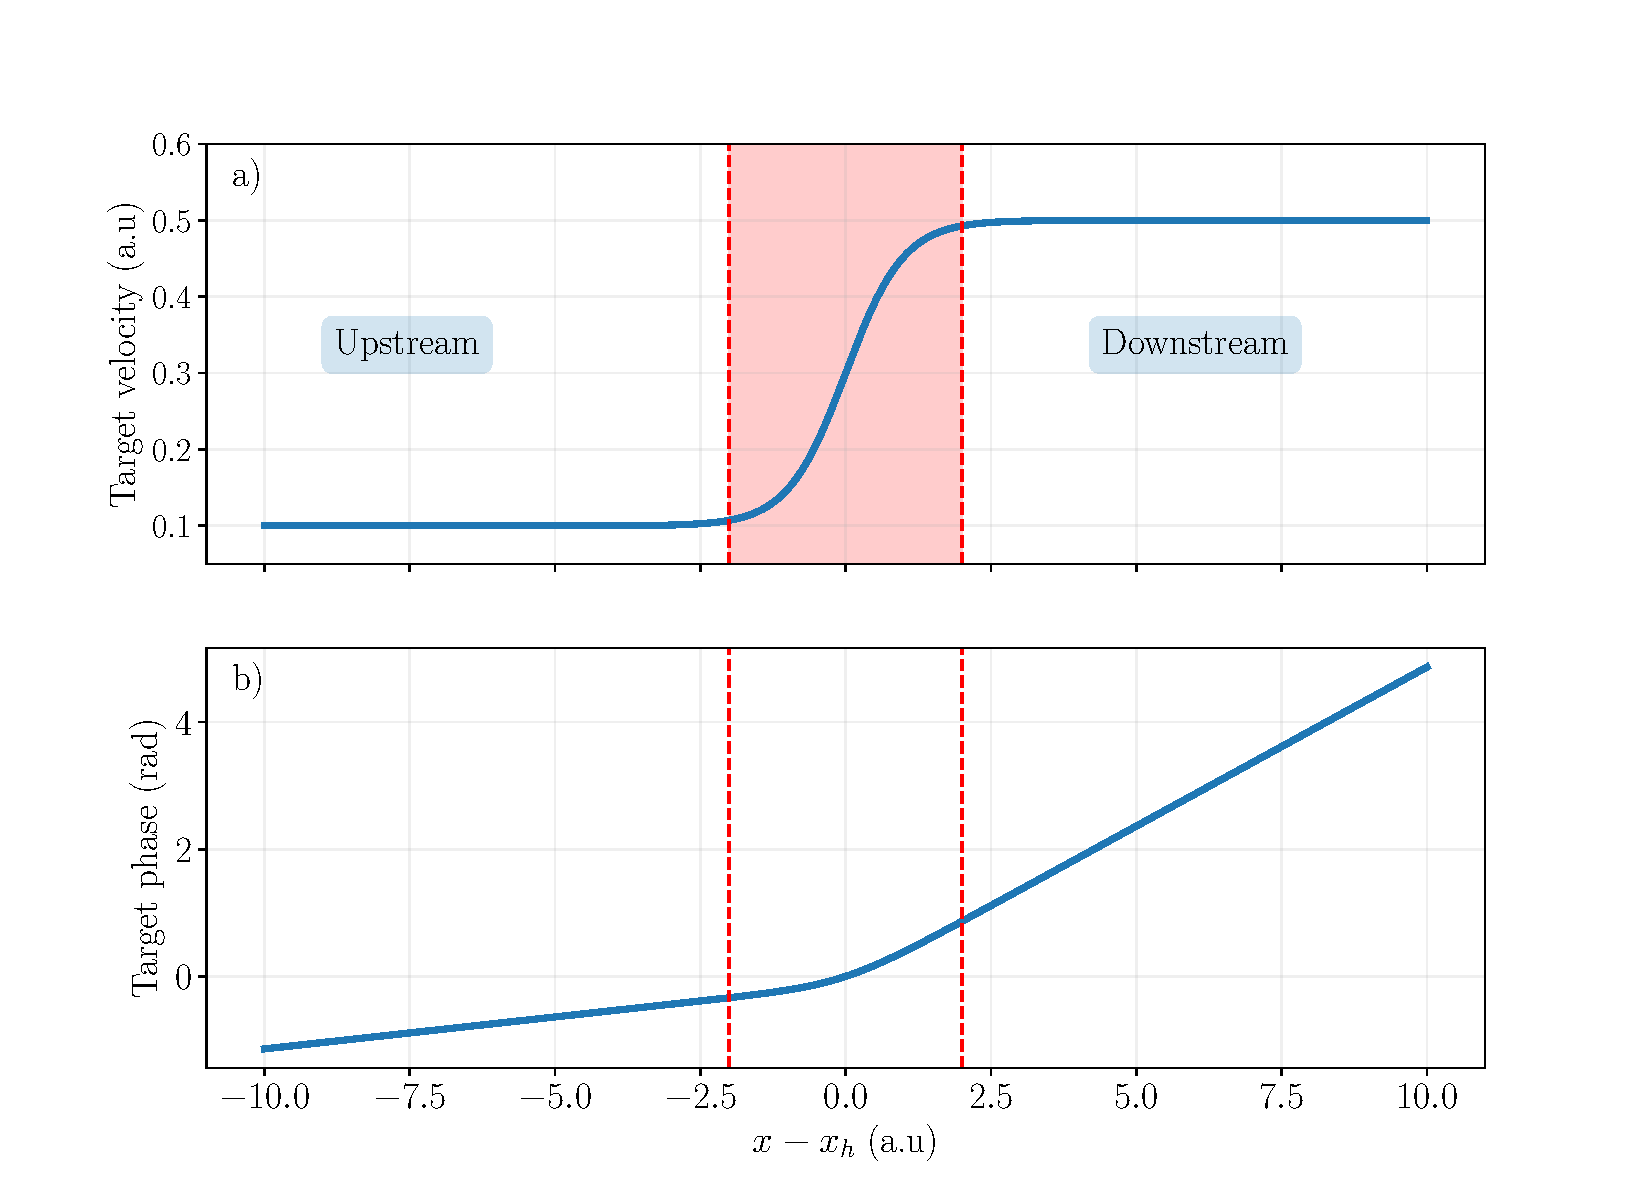
\includegraphics[width=1\textwidth]{chap_custom_st/fig/target_velocity.pdf}
    \caption{ a) Target velocity profile for input parametes $v_{up}=0.1$, $v_{d}=0.5$, $x_h=0$ and $w_h=1$ in arbitrary units. The red shaded area represent the 
    transition region. b) Corresponding phase profile to be imprinted on the pump laser.}
    \label{fig:target_velocity.pdf}
\end{figure}

Such a velocity profile show a great flexibility in the choice of the upstream and downstream velocities as well as the steepness and the position of the transition. From 
this, one can determine the phase that must be imprinted on the pump laser to generate such a flow profile by simple integration of \autoref{eq:target_velocity}, which gives :

\begin{equation}
    \phi(x) = \dfrac{m_{LP}}{\hbar} \int v(x) dx = \dfrac{m_{LP}}{\hbar} \left( \dfrac{v_{d}-v_{up}}{2} w_h \mathrm{ln}(\cosh(\dfrac{x-x_h}{w_h}))+\dfrac{v_{up}+v_{d}}{2}x \right).
    \label{eq:target_phase_profile}
\end{equation}
The latter is plotted in \autoref{fig:target_velocity.pdf} b). The derivative of this curve at position $x$ corresponds to the local wavevector of the pump laser, or equivalently, this curve provides a direct side view of the wavefront of the driving laser.
 Indeed, the wavefront is defined as the surface of constant phase of the beam. Notably, considering that the driving laser also possesses a wavevector along the $z$ direction, determined by the resonance conditions, the isophase surfaces of the total laser phase $\theta_{laser}$ are given by:  

\begin{equation}
    \begin{align}
    \theta_{laser}(r)&=k_zz+\phi(x)=cst \\
                      &=\frac{2\pi n_{cav} }{\lambda_0}z+\theta(x)= cst,
    \end{align}
\end{equation}

which is inverted as $z\propto \phi(x)$. Making a fluid with the wanted velocity field then boils down to be able to imprint the phase \autoref{eq:target_phase_profile} on the laser that resonantly excite the fluid. As we will see in the next section, this can be done with a Spatial Light Modulator (SLM). 

 A simplified scheme showing how printing the target wavefront in the sample plane create the desired flow.
To verify that the fluid has the expected phase we use an usual off axis interferometry method whose principle is explained in \autoref{sec:phase_measurement}
As an example, the measured phase corresponding to the mean field displayed in \autoref{fig:wavefront_shapping} b) is shown in \autoref{fig:phase_example}.
 
\begin{figure}
    \centering
    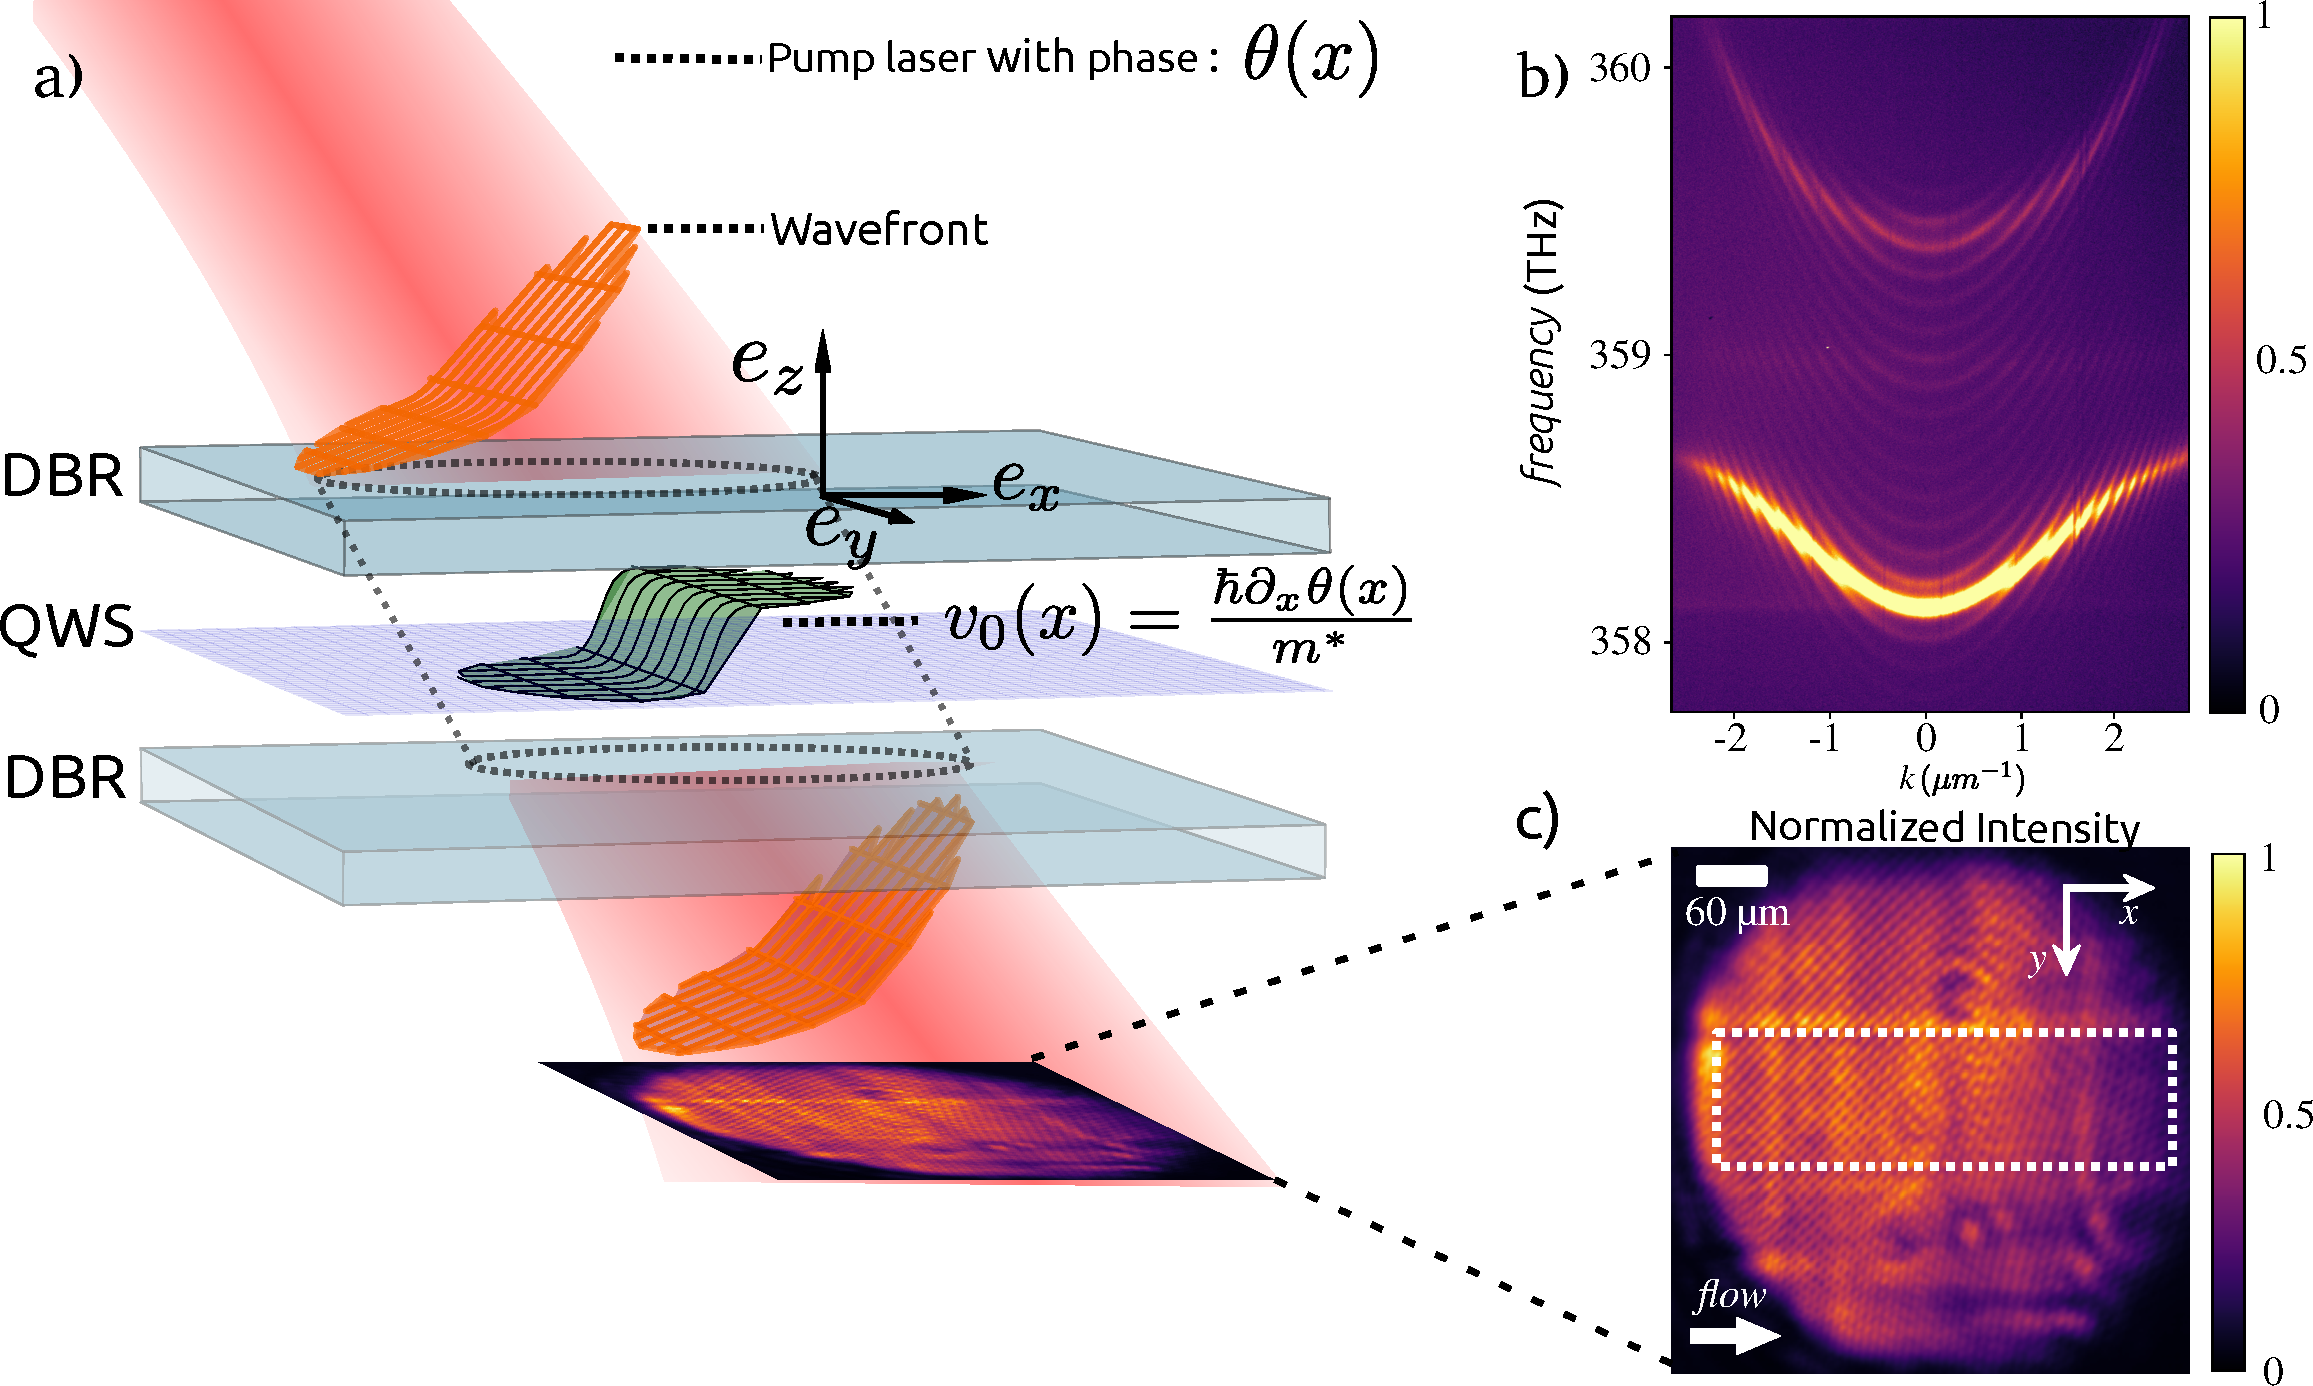
\includegraphics[width=1\textwidth]{chap_custom_st/fig/wavefront_shapping.pdf}
    \caption{Simplified scheme of the generation of a transonic fluid. a) The pump laser is shapped with the target phase profile and sent on the microavity The corresponding fluid velocity field is represented by the black surface lying on the Quantum Wells (QWs). c) The outgoing photons are collected and the sample 
    plane is imaged on a CCD camera to obtain the fluid density map.  b) Measured Lower and Upper polariton dispersion at the working point $C6-D6$ at which the experiment was run. By fitting this dispersions,
    the effective LP mass can be extracted $\mlp= 7.0 \times 10^{-35}$ kg}
    \label{fig:wavefront_shapping}
\end{figure}


\bigskip 

\textbf{Controlling the local intensity}. Being able to modify on demand the intensity of the pump laser along with the phase is also crucial since the polariton fluid density, and thus the regime of collective excitation, depends on the input intensity as explained in ??. 
Notably, if the system operates at the turning point of the bistability loop, it exhibits a linear collective excitation spectrum, and the speed of sound is directly linked to the detuning of the laser with respect to the lower polariton branch as $gn+g_rn_r=\delta(k_p)$. 
More generally, the possibility to move onto the higher branch of the bistability enables control over the gap opening in the Bogoliubov spectrum, transitioning from a linear spectrum to a masslike one.  
Once again, this can be achieved using the SLM by locally adjusting the height of the phase grating under the target phase profile, as explained in \autoref{sec:local_intensity}. This adjustment reduces the number of photons directed into the first diffracted order. This method is widely employed to create top-hat intensity profiles and is of significant interest in metrology and cold-atom experiments to minimize systematic effects \cite{top_metrology_2018}.  

\bigskip




To summarize, it is possible to generate and monitor fluid with arbitrary density and velocity flow by shapping the pump laser both in phase and intensity. We hence have a full optical way to create
effective space time on which we can study the propogation of collective excitation near the transition region.

\subsection{Effective 1D fluid}

So far, the description of the fluid both in velocity and density was one dimensionnal despite the fluid is actually a 2D system. This assumption
rely on the fact that the fluid wavefunction is invariant under translation in the $y$ direction in a given region of interest represented by the white dashed rectangle of \autoref{fig:phase_example}. This area is approximatively $130 \mu m$ long and $30-40 \mu m $ large. 
A cut of both the phase and density in the direction orthogonal to the propagation are shown in \autoref{fig:phase_example} b) and c). Periodic modulations are present because of back reflection on the protection screen of the camera sensor and are present even without passing through the sample. These modulation can be removed
upon fourier filtering which allow to compute the variation of the phase with respect to $2\pi$,  $\sigma_y^{ph}/2\pi$= 0.3\% as well as the relative intensity variation $\sigma_y^I/\langle I \rangle$ =3\%. As a consequence,
we can safely assume that the fluid is effectively 1D in the region of interest. This contrats with the work \cite{nguyen_acoustic_2015} previously mentionned. In the present configuration, the shape of the horizon is fixed by the phase of the exciting laser and can be tuned as will which is crucial to
study the effect of the horizon steepness on the emitted signals. Moreover, the presence of the pump laser in the downstream region brings a double advantage. First, the velocity of the fluid can be changed and doesn't depend on the interaction energy of the upstream region, allowing to study many fluid configurations.
Secondly, this experiment doesn't suffer from the exponential density decay that come with ballistic propagation \cite{long_range_ballistic_2013}. As a consequence, it is possible to probe the collective excitation spectrum in any region of the fluid with a high resolution pump probe spectroscopy method that we will describe in the next section. This 
 method depends on the response of the system to a weak perturbation. It is hence somehow proportionnal to the interaction energy of the fluid $gn$ and better suited to pumped fluid \cite{claude_high-resolution_2022}.

\begin{figure}[h]
    \centering
    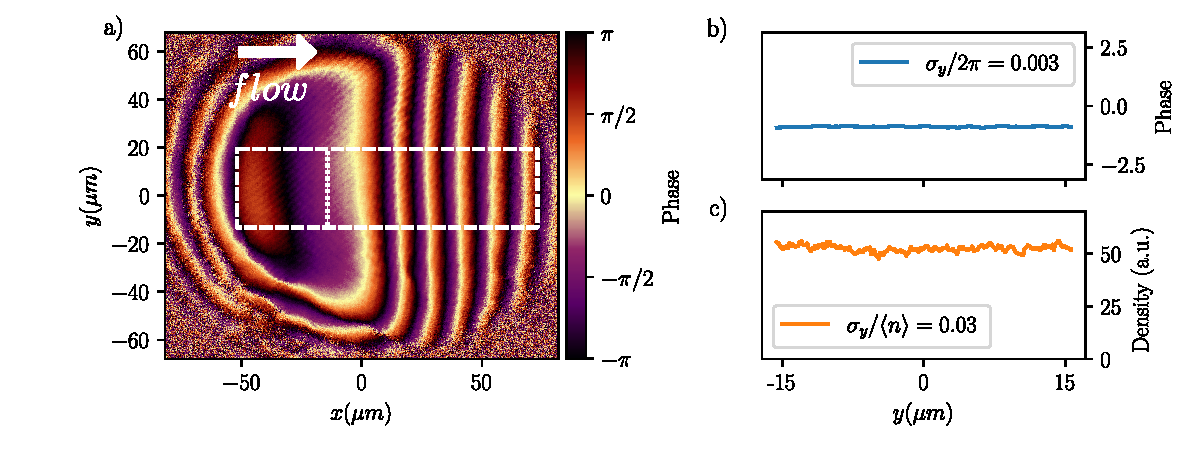
\includegraphics[width=1\textwidth]{chap_custom_st/fig/phase_example.pdf}
    \caption{a) Measured phase of the mean field shown in \autoref{fig:wavefront_shapping}.The curvature present in the upstream region is due to the non linear self focusing. The region
    on interest in which we assume translationnal invariance is represented by the white dashed rectangle. b)  Cut of the phase in the $y$ direction represented by the dotted white line in the rectangle. The variation to the phase with respect
    to $2\pi$ are equal to 0.3\%. c) Cut of the intensity of the mean field in the $y$ direction at the same location than b). The corresponding relative intensity variation is equal to 0.3\%.}
    \label{fig:phase_example}
\end{figure}

\section{Experimental spectroscopy of the collective excitation spectrum}

The analog of the Hawking radiation in a polariton fluid is the spontaneous emission of Bogoliubov modes from the horizon. When the system is operating at the turning point of the bistability the Bogoliubov spectrum 
is gapless and linear which enable to define a speed of sound $c_s = \sqrt{\hbar g n /\mlp}$ and speak without ambiguity of sonic excitation in the low wavevector limit. In this regime, the condition to observe negative energy modes coincide with the fluid being supersonic as explained in the previous chapter. 
However, creating a stable fluid at the turning point is quite challenging and the measurement of the spectrum linearity require experimental techniques that are hard to implement on a moving fluid \cite{claude_phd}. Nevertheless, linearity is not mandatory to observe Hawking radiation since 
it only requires the mixing between positive and negative energy modes which can be achieved without operating at the turning point. Besides, a gap opening in the Bogoliubov brings new physics on the table since it widen the study of quasi-particles creation to the case of massive particles. In this
section we discard the necessity to have sonic excitations and measure the presence of negative energy modes in a wide range of fluid configuration exploring different asymptotic velocities and horizon steepness.

\begin{figure}[h]
    \centering
    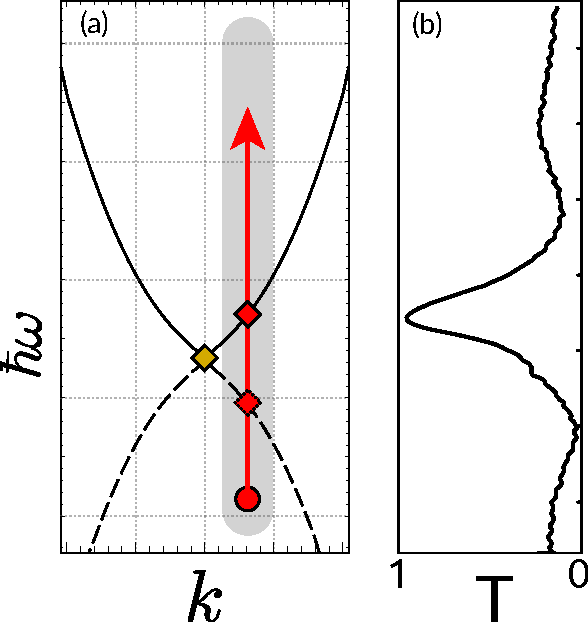
\includegraphics[width=0.3\textwidth]{chap_custom_st/fig/setup_bogoliubov.pdf}
    \caption{Simplified scheme of the pump probe spectroscopy method. a) At a given in plane wavevector represented by the red arrow, the probe frequency is scanned around the mean field frequency and is transmitted when it resonate with the bogoliubov branch. b) Typical transmission spectrum of the probe at the wevevector of a).}
    \label{fig:setup_bogo}
\end{figure}


\subsection{High resolution pump-probe spectroscopy method}

\label{sub:high_resolution_spectroscopy}

The measurement of the collective excitation spectrum consists in scanning the mean field resonance by looking at the transmission of a weak probe laser at the different incidence angles. First, polariton fluid is created with a driving laser as described in the previous section. A probe laser is then sent on the sample with a well defined incidence corresponding to an in plane wavevector as explained in \autoref{sec:photon}. The frequency of 
the probe is then scanned around the mean field frequency. When the perturbation frequency matchs these of the collective excitation, the probe create perturbations in the fluid with same energy and wavevector that ultimately escape the sample as photons. Frequency scans are then repeated for different incidence angles providing each time a transmission spectrum of the probe as shown in \autoref{fig:setup_bogo}. 
To make sure that we stay in the weak perturbation regime the intensity of the probe is set two order of magnitude below the pump. To collect only the signal emitted in the perturbation mode, a tunable pinhole is placed in the Fourier plane of the collection path and track the probe in-plane wavevector position to filter out the unwanted photons. Finally, the probe intensity is modulated at $f_{mod}$ in order to isolate its transmission from the very strong signal of the pump. The remaining ligth is then sent on
a photodiode connected to a Spectrum analyzer that demodulates the signal at $f_{mod}$ to obtain the transmission spectrum. At the end, all the scans are put together to reconstruct the full collective excitation spectrum as typically shown in \autoref{fig:homogeneous_fluid_bogo}.



\section{Experimental setup}
The setup used in this experiment is shown in \autoref{fig:set_up}. The sample is a microcavity consisting of three InGaAs quantum wells sandwiched between two highly reflecting planar GaAs-AlGaAs Bragg mirrors.
The quantum wells, separated by GaAs barriers, are located at the three antinodes of the cavity, which has a finesse on the order of 3000. A complete map of this sample 
 can be found at the end of this manuscript in \autoref{fig:sample_map} along with exciton-photon detuning measurements. This map enable to perform an experiment over several days at the same working point and overcome the problem due to daily cooling and warming procedures imposed by the open cycle cryostat. Furthermore, despite rigourous and exhaustive
 characterization of the sample, the quality of certain measurement can be substancially enhanced by looking phenomenologically the right working point fitted to the experiment. This being said, the experiment described in this chapter was run on the working point $C5-D6$.
 The set up is divided in three main paths, the pump path, the probe path and the collection path.


 \begin{itemize}
    \item \textbf{The pump path} represented by the blue box is used to create the stationnary states of the experiment. The polariton fluid is generated by a circularly polarized CW Ti:sapphire laser with a sub-MHz linewidth. This laser can be precisely frequency tuned around the LP resonance energy centered around 836 nm in our sample. An AOM 
    together with a Proportionnal-integral-derivative feedback on the AOM driving RF are used to stabilize the laser intensity and make sure the experiment is constantly runned at a single fluid density.
    The stabilized Gaussian beam is reflected on the spatial light modulator (SLM) which imprints the target phase $\theta_\mathrm{p}(x)=\int v_0(x)dx$ that determines the fluid velocity $v_0(x)$ at each point. The SLM plane is imaged in the plane of the cavity with two focal-length matched telescopes ($2f-2f$ configuration).
    \item \textbf{The probe path} represented by the red box is used to measure the collective excitation spectrum. The probe is another tunable CW Ti:sapphire laser with the same polarization than the pump beam. The probe is sent on the sample with a well defined incidence angle controlled by another SLM on which a tunable step blazed grating is imprinted. The frequency of
    the laser is scanned over $\SI{220}{\giga\hertz}$ around the mean field frequency and monitored by a high resolution wavemeter. An AOM and a Proportionnal-integral-derivative feedback are also used to both stabilize the intensity along the scan and apply a $f_{mod}=\SI{5}{\mega\hertz}$ intensity modulation.
    \item \textbf{The collection path} located after the sample is used to collect the signals emitted by the fluid. A microscope objective send the outgoing field on a 50:50 BS. One part is directed to an optical system to make the image both in real and momentum space of the field. For both lasers, a pick-up is made after their respective AOM to have a phase reference and perfom off axis interferometry measurement. Another part is sent to the apparatus described in \autoref{sub:high_resolution_spectroscopy} to measure the transmission spectrum of the probe. The tunable
    pinhole is made with a DMD placed in the fourier plan of a lense that send only photons arriving at the position of the pinhole to the collection photodiode. Taken 
    the relative size of the probe mode and the size of a pixel of the DMD, the resolution of the pinhole can go down to $\delta k = \SI{0.0005}{\per \micro\meter}$. The collection photodiode is then connected to a spectrum analyzer set in zero span at $f_{mod}$ to demodulated the signal and obtain the transmission spectrum of the probe. On both path
    as set of $\lambda/4,\ \lambda/2$ and $PBS$ to make polarization filtering of the signal.  
 \end{itemize}

 \textbf{Scan resonances analysis.} The shapes of the probe transmission and reflection peaks are directly related to the real and imaginary parts of the energy $\hbar \ombog$ of the Bogoliubov dispersion relation.
  If we consider plane wave like excitations

\begin{equation}
    \psilp(t) \propto \rmexp (-i \ombog t) = \rmexp \left (- i \re (\ombog) t \right ) \cdot \rmexp \left( \im (\ombog) t \right),
\end{equation}
one easily verifies by taking its temporal Fourier transform that its spectral density has the following Lorentz-distribution law

\begin{equation}
    I(\omega) = \abs{\psilp(\omega)}^2 \propto \dfrac{1}{ \left(\omega - \re(\ombog) \right)^2 + \left( \dfrac{\im(\ombog)}{2} \right)^2}.
\end{equation}

At each probe wavevector $k_{pr}$ the tranmssion spectrum $I_{k_{pr}}(\omega)$ is fitted with a Lorentzian function to extract the real and imaginary parts of the bogoliubov energy $\ombog(k_{pr})$

 \begin{figure}
    \centering
    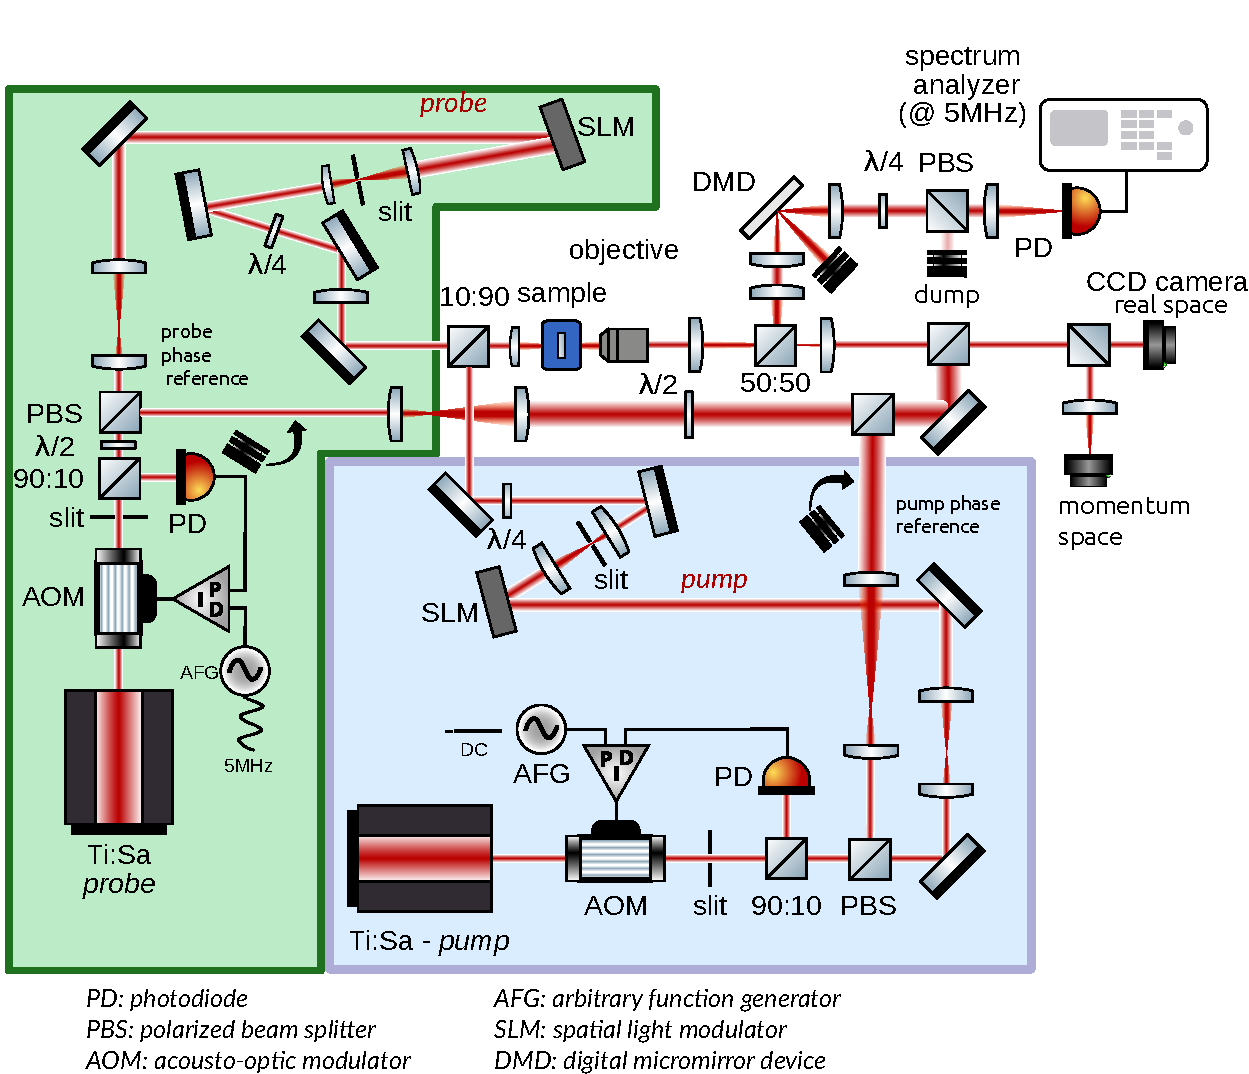
\includegraphics[width=1\textwidth]{chap_custom_st/fig/set_up_spacetime.pdf}
    \caption{Experimental setup}
    \label{fig:setup}
\end{figure}





\section{Experimental results}

\subsection{Homogeneous fluid}

To begin with, we first study homogeneous fluids with non zero velocities to see the effect of the doppler shift on the collective excitation spectrum. In this section,
the pump is a basic gaussian beam which creates fluid having a spatial extension of approximatively $150 \ \mathrm{\mu m}$. The input angle of the pump
is controlled in the same way as the probe by printing a tunable step blazed grating on the SLM. In each measurement, the effective detuning 
$\delta(k_p)=\omega_p -\omlp^0- \hbar k_p^2/2\mlp$ is high enough to be in the bistable regime and the input pump intensity is chosen so the system operate on the higher branch of the hystersis curve quite far from the turning point. 
The probe is set to be two order of magnitude weaker than the pump whith the same spatial extension and polarization.

\bigskip

\textbf{Direct normal branch measurement.} We create a set of homogeneous fluid with increasing in plane wavevectors $k_p$ while keeping the pump frequency constant. 
For each fluid, we use the pump probe spectroscopy method to measure the probe transmission spectrum as shown on \autoref{fig:homogeneous_fluid_bogo}. 
The DMD is programmed to display pinholes that track the wavevector of the probe laser along the scans. In this case the system measure the direct transmission of the probe. The first measurement a) is made with the pump laser turned off which means in the absence of interactions within the sample.
The probe transmission then scan the bear cavity resonances and recover the parabolic shape at low wavevector of LP branch. From this measurement we extract the detuning between the pump laser and the LP branch at zero wavevector
 $\delta(0) = \SI{33}{\giga\hertz}$. 
 The blueshift due to interaction lift the dispersion a) to higher energies whereas the doppler shift modifies the resonances according to 
 $\omega' = \omega + \vbf_p\delta \kbf$ where $\vbf_p$ is the fluid velocity $\vbf_p = \hbar \kbf_p/\mlp$.  As the fluid velocity increases, the branch is bended and moved toward the pump wavevector. 
 For $k_p\geq 0.3$ we already see some resonances lying under the pump energy. As explained in the previous chapter, the energy sign of a collective mode is given by :
 
 \begin{equation}
    \mathrm{sign}(E)=\mathrm{sign}(\omega_\mathrm{B})\times \mathrm{sign}(Q_{\phi}),
 \end{equation}
 
where $Q_{\phi}$ is the norm of the mode defined in \autoref{eq:norm} and $\mathrm{sign}(\omega_\mathrm{B}$ is taken with respect to the pump energy. Since the normal branch has a positive norm, the resonances located
below the pump frequency are negative energy modes. As it can be seen, the ghost branch is not visible through direct excitation. This feature has a double origin : first the ghost branch is not optically resonant with the cavity which makes photon injection difficult at its energy. Secondly,
the bogoliubov coeffecient $v_k$ of the negative norm branch is very small compared to $u_k$.  In the presence of
a coherent state like the probe, the populations then scale as $v_k^2 |\alpha|^2\ll u_k^2|\alpha|^2$ where $\alpha$ is the intracavity amplitude of the probe. 

\begin{figure}[h!]
    \centering
    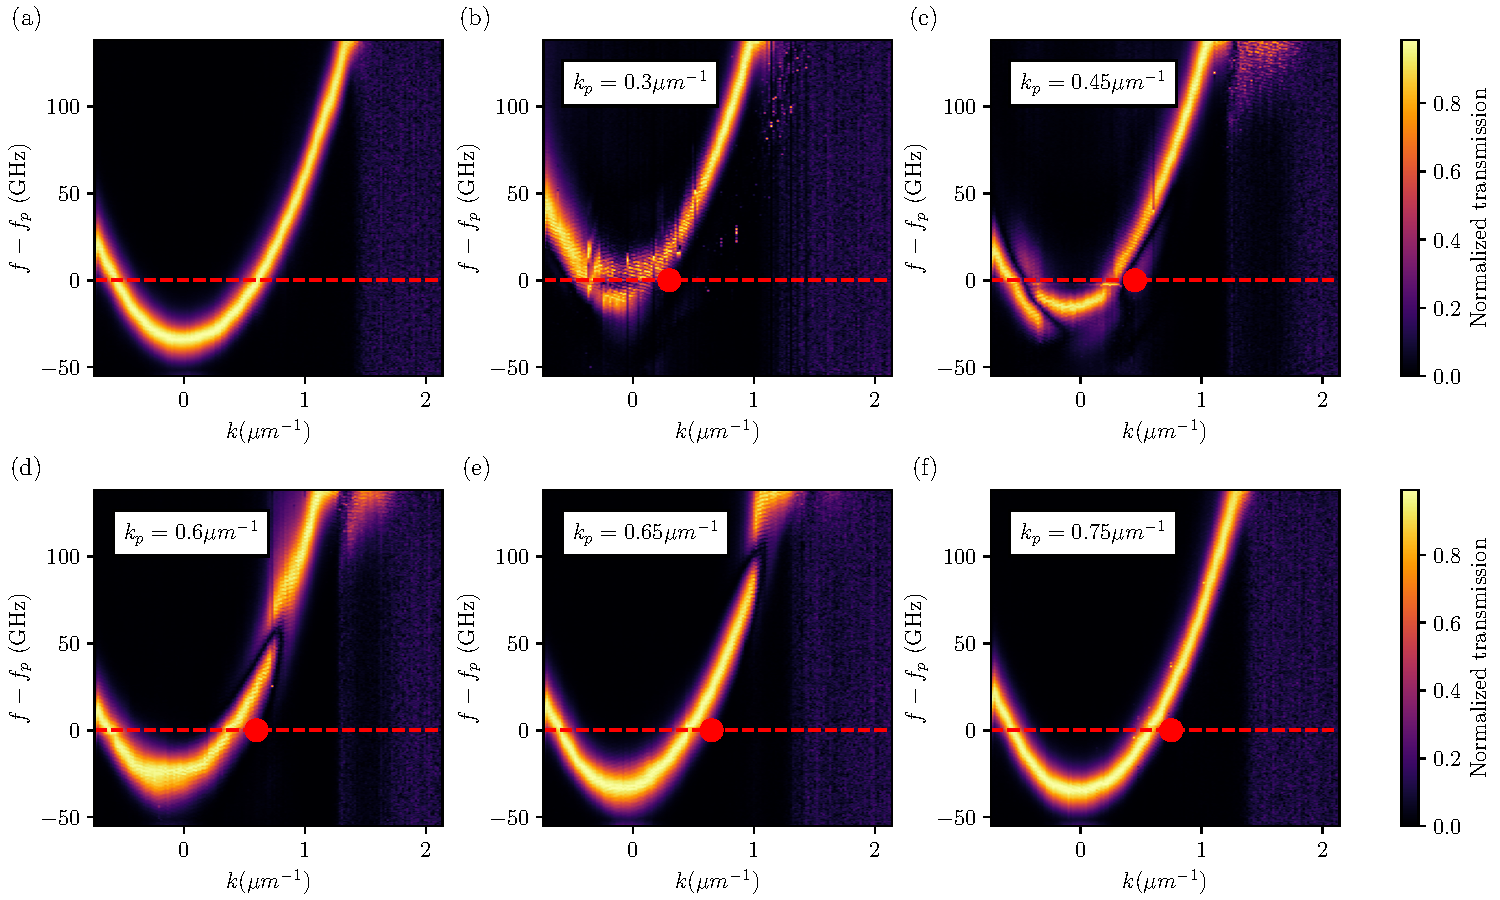
\includegraphics[width=1\textwidth]{chap_custom_st/fig/homogeneous_doppler.pdf}
    \caption{a) Bear cavity dispersion measurement with the pump probe spectroscopy method in the absence of fluid. 
    The parabolic shape of the Lower Polariton branch is recovered.  
    The red dashed line represent the mean field frequency that was kept constant for all the measurements. 
    From this we can measure the detuning between the pump laser and the LP branch at $k=0$,
     $\delta(0) = \SI{33}{\giga\hertz}$. b),c),d),e) and f) measured Bogoliubov normal branches for homogeneous fluid with velocities 0.75, 0.98, 1.23, 1.29 and $\SI{1.43}{\micro \meter \per \pico \second}$ respectively, corresponding 
    to the pump wavevector values in the inset of each figure.}
     
    \label{fig:homogeneous_fluid_bogo}
\end{figure}

\bigskip

 \textbf{Ghost branch indirect measurement.} To overcome the difficulty to directly excite the ghost branch, we take advantage of the strong linearities of the system to induce population
 through four wave mixing process. Indeed, because of the bosonic nature of bogoliubov excitations, occupation of the normal branch in the probe wavevector mode should stimulate the parametric conversion of two pump polaritons into a bogoliubov pair with opposite wavevectors and energies with respect to the pump, namely :

 \begin{subequations}
    \begin{align}
    (k_p, k_p) &\rightarrow (k_p+\Delta k, k_p-\Delta k),\\
    (\omega_p, \omega_p) &\rightarrow (\omega_p+\Delta \omega,\omega_p- \Delta \omega).
    \end{align}
 \end{subequations}
The emission in the ghost branch is then boosted by a factor $(u_kv_k)^2|\alpha|^2$ \cite{I_frerot_PRX_2023}. In practice, this measurement
can be done by changing the positions of the tunable pinhole so it track wavevector opposite to the probe with respect to the pump. More precisely,
when a scan at $k_{pr}=k_p+\Delta k$ is made, the pinhole is set at $k_{pr}=k_p-\Delta k$ to collect the signal emitted in the conjugated mode. 

\bigskip

Here we create again a homogeneous fluid with wavevector $k_p =0.6 \mu m^{-1}$. We then 
perform direct measurement of the normal branch and indirect measurement of the ghost branch. The results are shown in \autoref{fig:homogeneous_fluid_bogo_ghost} \textbf{a)} and \textbf{b)} respectively.  The modulations on the right side of the direct measurement come from interferences in the substrat of the sample
that act as a low factor Fabry Perot \cite{claude_phd}. Each scan is normalized to its own maximum for the sake of clarity but 
the strength of the indirect signals is approximatevily $1-10\%$ of the direct one. The noise present on several scan of b) corresponds to parasitic signals coming from other scatterings process that may send photons at the position of the pinhole and that, in the case of direct measurement, are negligible with respect to the resonance. The reason why the ghost branch doesn't appear as the symetric of the normal branch 
is because the axis $k$ and $f-f_p$ represent the wavevector and frequency of the injected probe and not the emitted signal. However, the pinhole positions first ensure us that the signal is emitted in the opposite wavector mode. To verify that it is also symetric in frequency, we send the photons collected by the pinhole 
into a spectrometer to measure their energy. This two test enable to confirm that the signals taken through indirect measurement in \textbf{b)} indeed come from the ghost branch. As a consequence, it is possible  to symetrize the indirect data around the pump wavevector and energy to plot the full collective excitation spectrum shown in \autoref{fig:homogeneous_fluid_bogo_ghost} \textbf{c)}. First, one can check that the two branches 
are indeed symetric with respect to the pump represented by the red dot.
\begin{figure}
    \centering
    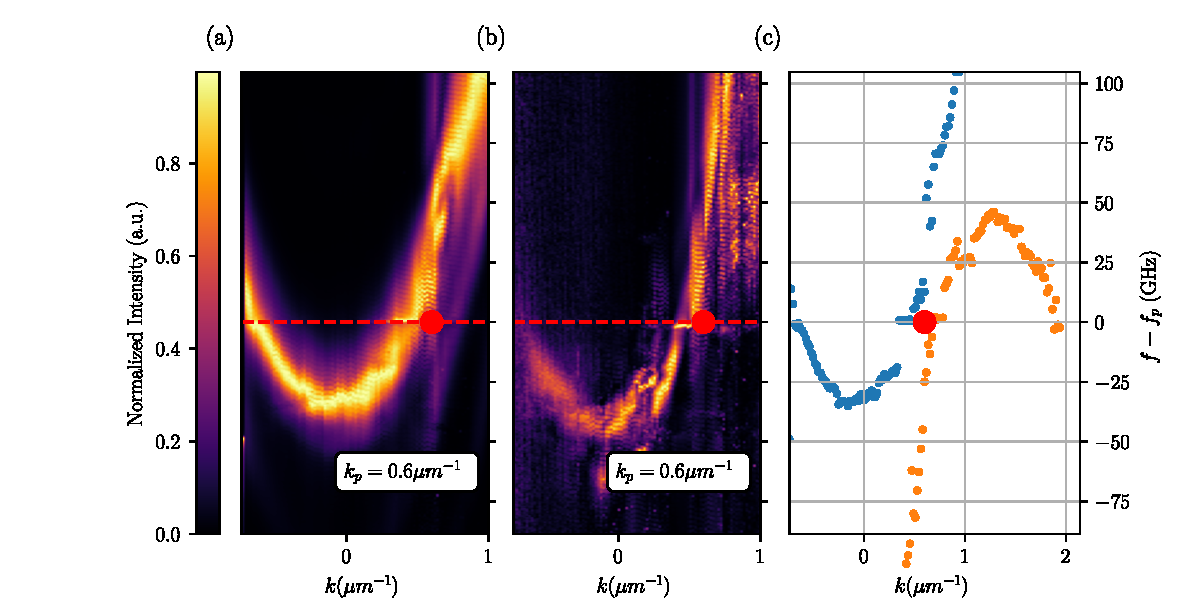
\includegraphics[width=1\textwidth]{chap_custom_st/fig/supersonic_homogenous.pdf}
    \caption{\textbf{a)} Direct measurement of the normal branch of the Bogoliubov spectrum for a homogeneous fluid with in plane wavevector $k_p=\SI{0.6}{\per \micro \meter}.$ \textbf{b)} Indirect measurement of the ghost branch of the Bogoliubov spectrum for the same fluid.
    c) Extracted resonance energy for each probe wavevector. The blue point are extracted from the direct measurement and correspond directly to the resonances of \textbf{a)}. The orange points are extracted from the indirect measurement. Each couple $(k_{pr}, \omega)$ extracted from b) is symetrized around the pump position in phase space $(k_p, \omega_p)$ to account for 4wm process.}
    \label{fig:homogeneous_fluid_bogo_ghost}

\end{figure}

Once again this measurement is an additionnal proof that when the fluid velocity is high enough, negative energy modes can be excited on both positive and negative norm branches.
It's worth noticing that no effort were put in this experiment to reach the turning point of the bistability loop which didn't prevent the observation of negative energy modes. This ease 
the experimental constraints to observe Hawking radiation in a polariton fluid and in fact widen the initial analogy that was made for sonic excitation in a supersonic fluid. More precisely it can be refomulated as follows :
a fluid exhibiting a sharp transition between a region with positive energy modes, and another with negative energy modes available, should experience correlated emission of Bogoliubov modes at the transition.
These modes are not necessarly phonons and the velocity one has to exceed to observe them is not necessarly the speed of sound, but rather a critical velocity that depends more generaly on the fluid parameters.
Although this statement seems unclear with respect to the sonic version, it is actually more general and broaden the range of experimental configurations at which particle creation can be observed. In the following 
we will rather speak of trans critical flow and critical velocity instead of "sonic".






\subsection{Smooth transition geometry}

We first study a smooth transition between the sub- and supercritical flow regions.
We implement the target velocity profile \autoref{eq:target_velocity} with a transition width $w_\mathrm{H}=\SI{20}{\micro\meter}$. 
We study three profiles, with three values for the up- and downstream flow velocities $v_\mathrm{u}$ and $v_\mathrm{d}$.
All the measurements are made with $\delta(0)=\SI{56}{\giga\hertz}\rightarrow \hbar\delta(0)= \SI{0.2}{\milli \electronvolt}$.
At this detuning the system is in the bistable regime in both the upstream and downstream regions with a spatial extension of $\SI{120}{\micro \meter}$.
For each configuration, the phase of the created fluid is measured by off-axis interferometry as described in \autoref{sec:phase_measurement}. By unwrapping the phase profile, as the one typically shown in \autoref{fig:smooth_transition} \textbf{a)}, and taking the gradient in the $x$ direction, we obtain the fluid velocity profile $v(x)$.
The measured velocity profiles are represented by the solid lines in \autoref{fig:smooth_transition} \textbf{b)} showing three different asymptotic downstream velocities $v_\mathrm{d}$ with a single upstream velocity $v_\mathrm{u}$. 
To selectively measure the upstream or downstream region the diameter of the probe beam is reduced to half the spatial extension of the fluid and the probe focused on the region of interest. The corresponding excitation spectra are shown in \autoref{fig:smooth_transition} \textbf{c)-f)}. 
The upstream region is shown in \autoref{fig:smooth_transition} \textbf{c)} and the downstream regions in \autoref{fig:smooth_transition} \textbf{d)-f)}.

\bigskip

\subsubsection{Speed of sound measurement} Eventhough the system doesn't operate in a regime of sonic collective excitation we call $c_s=\sqrt{\hbar g n/\mlp}$ the speed of sound. The value of $gn$ is extracted 
from the simultaneous fit of the normal and ghost branch of each spectrum with the bogoliubov dispersion relation :

\begin{equation}
    \label{eq:lfbogo}
    \begin{split}
        \ombog^{\pm}(\delta k)= -\frac{i\gamma}{2}+ v_0(x) \delta k(x)\,\pm \\\sqrt{\left(\frac{\hbar \delta k(x)^2}{2m^*}-\delta(k_p) +2gn(x) +g_\mathrm{r} n_\mathrm{r}    \right)^2-(gn(x))^2},
    \end{split}
\end{equation}
with $\delta k(x)=k-k_p(x)$. The only unkwonw parameters in this equation are $gn$ and $g_rn_r$. However by taking the steady states solution of the Gross Pitaevskiii equation coupled to a reservoir \autoref{eq:generalized_GPE} we obtain $n_r\propto n$.
Based on the work \cite{claude_phd,claude_high-resolution_2022} made on the same sample and the assumption that the reservoir contribution depends on the exciton-photon detuning. We use the value $g_rn_r\approx 1.8gn$ of work \cite{claude_phd} and end 
with a single free parameter $gn$ to fit the spectra. The fit are represented by the colored dashed line in \autoref{fig:smooth_transition}. The output of the fit gives in fact a value of $gn(r_{pr})$ where $r_{pr}$ is the position of the probe. However, this value can serve 
as calibration to reconstruct the full $gn(r)$ profile. Indeed we can safely assume that the output measured intensity is proportionnal to the 
fluid density as $I_{out}(r)=a n(r)$ and that $a$ is a constant that depend on the exciton photon detuning through the hopfield coefficients and complex 
cavity parameters. Nonetheless, given the spatial extension of the fluid with respect to the wedge of the sample $\SI{0.04}{\micro \electronvolt \per \micro \meter}$, these paramateres can be considered as constant in the region of interest.
We can then calibrate the speed of sound measurement through :

\begin{equation}
    \label{eq:speed_of_sound_calib}
    c_\mathrm{s}(r)=\sqrt{\frac{I_{out(r)}}{I_{out}(r_{pr})}}c_s(r_{pr}).
\end{equation}

The $c_s(x)$ map obtained for the different configurations are represented by the dashed lines in \autoref{fig:smooth_transition} b). The speed of sound is found to be quite constant which yields a smooth transition betwe en the upstream and downstream regions. 

\bigskip

\begin{figure}
    \centering
    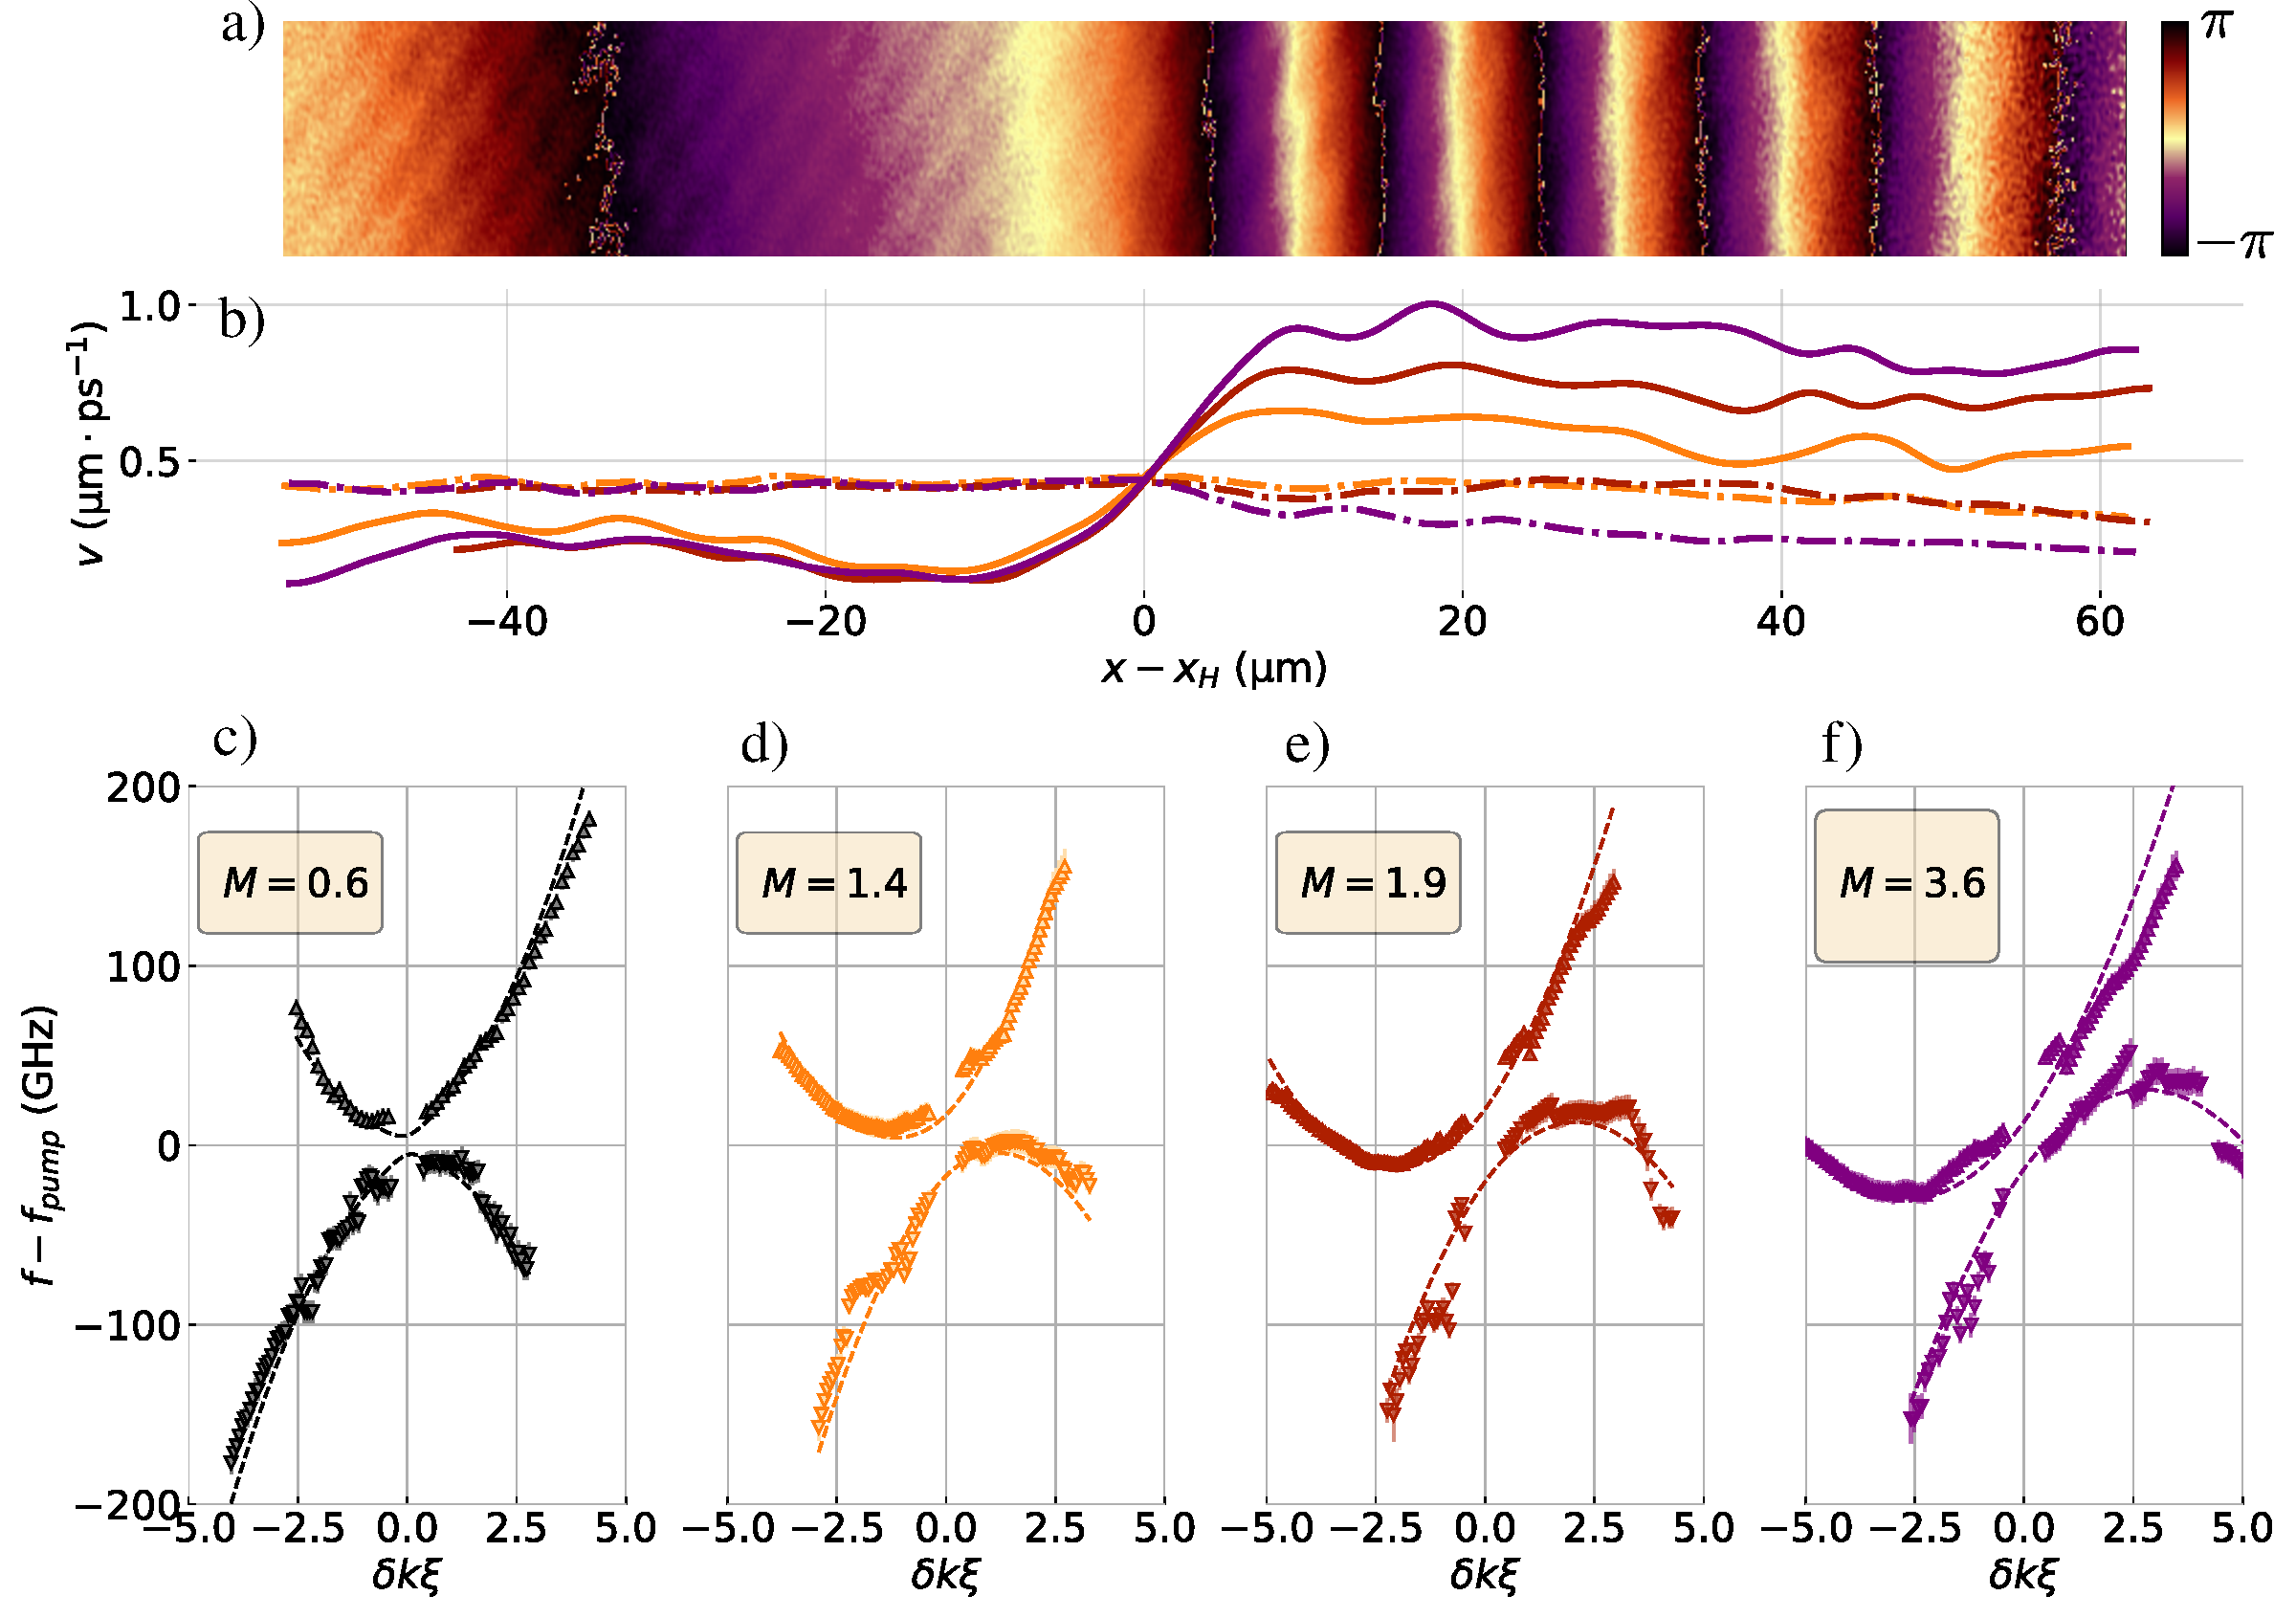
\includegraphics[width=1\textwidth]{chap_custom_st/fig/bh_smooth.pdf}
    \caption{\textbf{Smooth horizon}.
    \textbf{a)} Typical measured phase of the fluid $\theta(x)$ inside the region of interest as defined in \autoref{fig:phase_example}.
    \textbf{b)} Fluid velocity profiles.
    Solid lines, $v_0(x)$; dot-dashed lines, $c_\mathrm{s}(x)$. Orange, $M_\mathrm{u}=0.6$ and $M_\mathrm{d}=1.4$; red, $M_\mathrm{u}=0.4$ and $M_\mathrm{d}=1.9$; purple $M_\mathrm{u}=0.5$ and $M_\mathrm{d}=3.6$.
    \textbf{Excitation spectra} Eq.~\eqref{eq:lfbogo}: \textbf{c)} typical upstream region; \textbf{d)}-\textbf{f)} downstream region.
    Up-triangles, positive-norm branch $\omega_\mathrm{B}^+$; down-triangles, negative-norm branch $\omega_\mathrm{B}^-$; dashed lines, fit with free parameter $gn$. Error bars mostly come from the uncertainty in the determination
    of the center of the lorentzian function used to fit each scan.
    \label{fig:smooth_transition}}
\end{figure}




\subsubsection{Critical velocity} In conservative fluids, sub- and supercritical flows are discriminated by the Mach number $M\coloneqq v_0/c_\mathrm{s}=1$.
Instead, in our driven-dissipative fluid, the minimum velocity to have a supercritical dispersion is larger than $c_\mathrm{s}$.
As a result, the condition $M=1$, which defines the acoustic horizon in the hydrodynamic limit does not necessarily coincide with the condition to excite negative energy waves in the system. In other words the position at 
which the velocities exceed $c_\mathrm{s}$ in \autoref{fig:smooth_transition} b) doesn't define the horizon of the fluid. Indeed, when the system doesn't operate at the turning
point of the bistability we have $gn>\delta(k_p)-g_rn_r$, which opens a gap in the dispersion. We rewrite the dispersion in the laboratory frame in a form that allows to easily identify the effect of the gap on the spectrum,


\begin{align}\label{eq:lfbogom}
    \omega^\pm_\mathrm{B}(\delta k)=&v_0(x) ,\delta k(x)-i\frac{\gamma}{2}\nonumber\pm\Biggl[\left(\frac{\hbar\delta k(x)^2}{2 \mlp}\right)^2+\frac{\hbar \delta k(x)^2}{\mlp}(2g n_0 - \delta(k_\mathrm{p})+g_\mathrm{r}n_\mathrm{r})\\
    &\,\,+(g n_0 - \delta(k_\mathrm{p})+g_\mathrm{r}n_\mathrm{r})(3 g n_0 - \delta(k_\mathrm{p})+g_\mathrm{r}n_\mathrm{r})\Biggr]^{-1/2}\nonumber\\
    =&v_0(x) \delta k(x)-i\frac{\gamma}{2}\,\pm\sqrt{\left(\frac{\hbar\delta k(x)^2}{2 \mlp}\right)^2+c_\mathrm{B}^2\delta k(x)^2+\mbogo^2c_\mathrm{B}^4}
\end{align}

where we defined :
\begin{subequations}
    \label{eq:m_bog}
    \begin{align}
    c_B & = \sqrt{\dfrac{\hbar(2gn_0- \delta(k_p)+g_\mathrm{r}n_\mathrm{r})}{\mlp}},\\
    \mbogo&=\mlp\dfrac{\sqrt{(gn_0- \delta(k_p)+g_\mathrm{r}n_\mathrm{r})(3gn_0- \delta(k_p)+g_\mathrm{r}n_\mathrm{r})}}{(2gn_0- \delta(k_p)+g_\mathrm{r}n_\mathrm{r})}.
    \end{align}
\end{subequations}

These two quantities have a well defined physical meaning as follows. 
On the one hand, $\mbogo c_\mathrm{B}^2$ is the energy of $k=0$ modes of $\phi$, introducing a mass gap which vanish when the system operates at the turning point of the bistability.
On the other hand, ?? is a hyperbolic PDE whose characteristic curves in a fluid at rest are given by $|\pmb{x}|=c_\mathrm{B} t$. These characteristics limit the speed at excitations $\phi$ can propagate information, defining the soundcones in full analogy to light cones. However, due to the mass gap, the speed of propagation of excitations of $\phi$ is $v_{\rm g}=d\omega/dk\leq c_\mathrm{B}$. 
The latter can be seen as the limiting speed of propagation of $k\to\infty$ perturbations. This is also in full analogy to propagation of modes of a massive relativistic scalar field, which travel at subluminal speeds, reaching only the speed of light in the limit of infinite momentum.
From \autoref{eq:lfbogom} we see that the field mass $\mbogo$ increases $\abs{\mathrm{Re}(\omega_\mathrm{B}^{\prime\pm})}$ at all $k$, meaning that the critical velocity to have a Doppler effect large enough to excite negative energy  waves is larger than $c_s$.
The value of the critical velocity $v_c=\hbar k_c/\mlp$ at which negative energy waves become available at positive frequency can be computed as follows. 


For $k_p>k_c$, there will be negative norm modes available at positive frequencies, and there will be two values $\delta k_{1,2}$ at which each dispersion branch intersects the horizontal axes. These $\delta k_{1,2}$ depend on the value of $k_p, gn$ and $g_rn_r$. 
The critical wavenumber $k_c$, and correspondingly the critical velocity $v_c=\hbar k_c/\mlp$, is obtained when the two intersection points merge, so that $\delta k_1=\delta k_2=\delta k_0$.
In practice, we compute numerically the  normal branch $\omega_B^+(\delta k)$ spectrum for different values of $k_p$ and $gn$ while keeping the zero momentum detuning constant 
and equal to $\delta(0)=\SI{56}{\giga\hertz}$ as in the experiment. On each computed spectrum, we verifiy if it exhibits negative frequency values. We obtain the map  \autoref{fig:critical_velocity_map}.
 if a fluid with given velocity and interaction energy is super-critical. The points c), d), e) and f) correspond to the measured spectrum of \autoref{fig:smooth_transition}.
As it can be seen, the upstream region and downstream region with the smaller velocity don't lie in the super-critical regime whereas e) and f) do. This is in agreement with the fact that the critical velocity is larger than the speed of sound since 
all the regime yielding super-critical flows are located on the right side of the black dashed line corresponding to the acoustic case $c_s = \hbar k_p/\mlp=\sqrt{\hbar gn/\mlp}$. Besides, the map predicts well that configuration d) is subcritical despite a 
Mach number $M_d=1.34$ greater than one.

\bigskip

\textbf{Cutoff spatial frequency.} The absence of experimental data points at wavevectors $\delta k < 0.10 \mu m^{-1}$ is a consequence of the finite size 
of the probe beam $\delta_x = \SI{60}{\micro\meter}$ which fixes the spatial extension of the probe in momentum space
 scaling as $2\pi/\delta_x=0.10 \mu m^{-1}$. At very small wavevector, the probe and its conjugated counterpart start to overlap and photons
 coming from both branches are collected by the pinhole. This prevent the effective discrimination between the two modes in the ouput signal of the photodiode. In practive the 
 cutoff frequency is computed by a simple optical Rayleigh criterion stating that two points are resolved if the distance between them is larger than the FWHM of the point spread function.
In our case this directly gives $\delta k_{cut} = 2\pi/\delta_x= 0.10 \mu m^{-1}$.

\begin{figure}
    \centering
    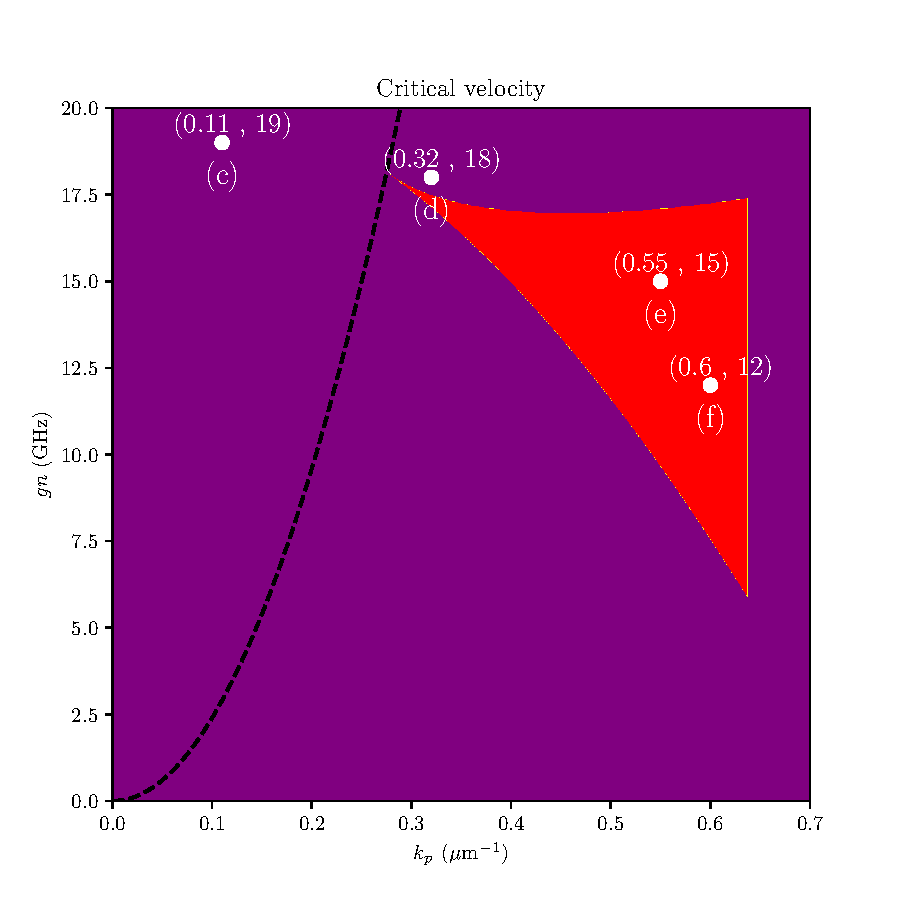
\includegraphics[width=0.8\textwidth]{chap_custom_st/fig/critical_velocity_map.pdf}
    \caption{Critical velocity map as a function of $k_p$ and $gn$ while the reservoir contribution was fixed as $g_rn_r\approx 1.8=gn$. For each couple $(k_p,gn)$ the bogoliubov spectrum \autoref{eq:lfbogo} is computed : red points correspond to super critical flows and purple point to sub-critical flows.
    The points c), d), e) and f) correspond to the measured spectrum of \autoref{fig:smooth_transition}. The black dashed line represent the acoustic case where the critical velocity coincide with the speed of sound $c_s = \hbar k_s/\mlp=\sqrt{\hbar gn/\mlp}$ }
    \label{fig:critical_velocity_map}
\end{figure}

\subsubsection{Paired emission frequency range}

The paired emission of correlated mode at the horizon require the mixing of positive and negative energy modes. Consequently the finite velocity in the downstream 
sets a maximum frequency at which the effect can occur \cite{jacquet_hawking_2019}. This frequency is given by the maximum energy of the negative energy modes that can be excited in the downstream region and is ultimately 
set by the asymptotic downstream velocity $v_d$ and the interaction energy $gn$. Increasing this range result in a larger number of correlated pairs emitted and is expected to enhanced
the overall correlation signal \cite{jacquet_hawking_2019}. 
In \autoref{fig:hawking_range} we plot the analitycal bogoliubov dispersion corresponding to the measurement of \autoref{fig:smooth_transition} c), e) and f).  Paired emission is then possible in the red range of \autoref{fig:hawking_range}  where negative energy modes
can mix with the positive energy mode of the upstream spectrum, located outside the gap represented in blue.

The overall frequency range at which hawking emission is possible is given by :

\begin{equation}
    \begin{align}
    \Delta \omega_H& \coloneqq  2\omega_{max}- \Delta\omega_{gap}
    \end{align}  
    \label{eq:hawking_range}
\end{equation}

where $\omega_{max}$ is the maximum energy of the negative energy modes that can be excited in the downstream region and $\Delta\omega_{gap}$ the width 
of the gap in the upstream spectrum. We measure $\Delta \omega_H$=6 GHz for the e) configuration and 30 GHz for the fastest flow. 
Hence by changing the asymptotic downstream speed our system enable to tune the number of states available for paired emission. Let us now 
see that we can control another crucial parameter of the hawking radiation, the steepness of the horizon.

\begin{figure}
    \centering
    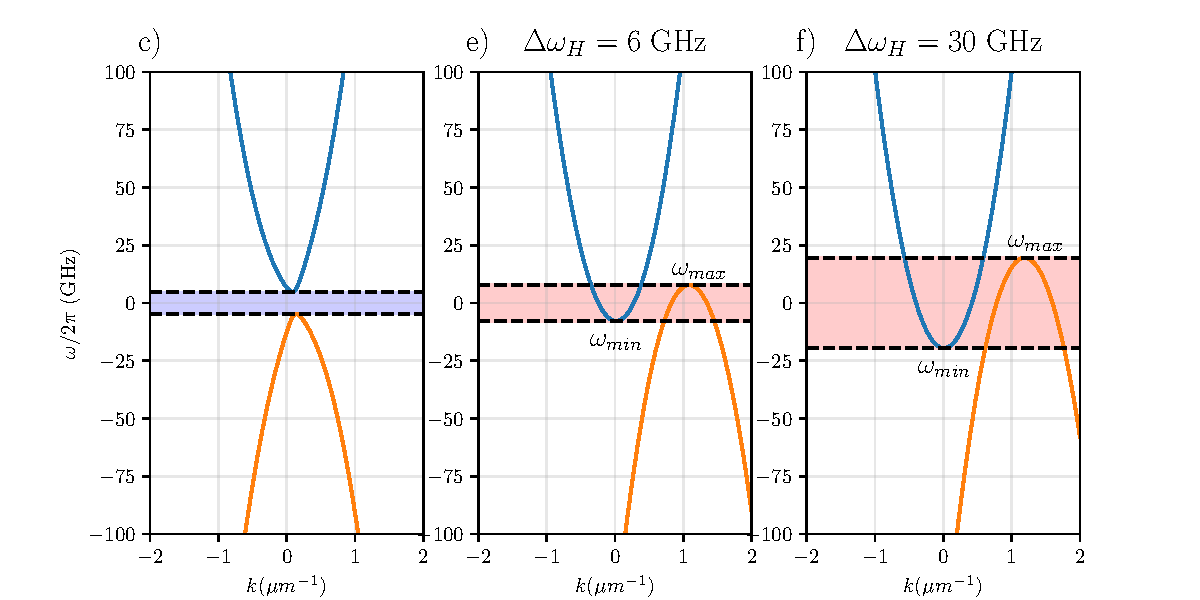
\includegraphics[width=0.8\textwidth]{chap_custom_st/fig/max_freq_hawking.pdf}
    \caption{c) , e) , f) analytical bogoliubov dispersion corresponding to the fit of \autoref{fig:smooth_transition} c), e) and f). The red range in e) and f) represent the frequency range at which negative energy modes
    are available that can mix with the positive energy modes outside the gap represented in blue whose value $\Delta \omega_H$ are displayed above each plot.}
    \label{fig:hawking_range}
\end{figure}

\subsection{Steep horizon geometry}

The sharpness of the transition is a crucial parameter to study the strength of correlation of the emitted modes. It can be inferred by the quantity :
\begin{equation}
    \kappa \coloneqq \frac{1}{2c_\mathrm{s}(x)}\frac{d}{dx}[v^2_0(x)-c^2_\mathrm{s}(x)]|_{x_\mathrm{H}},
    \label{eq:steepness}
\end{equation}
the hydrodynamic equivalent to surface gravity \cite{barcelo_hawking-like_2006}. However the discussion in the previous section 
pointed out that the position $x_H$ at which the fluid velocity exceed the speed of sound doesn't define the horizon of the fluid, the derivative
in the definition of $\kappa$ should then rather be taken at the position where the critical velocity is reached and involve the critial velocity instead of $c_s$.
In practice this brings only a negligible correction to the value of $\kappa$. 

\bigskip

\textbf{Increasing the surface gravity.}
The steepness of the horizon can be tuned in two ways. First, by reducing the width of the transition $w_H$ in the target velocity profile.
Second, by taking advantage of the dependance of the bistability cycle on the effective detuning $\delta(k_p)$.
As shown in \autoref{fig:optical_bistability} b) the value of $gn$ with a fixed input intensity scales increases linearly with the effective detuning until the turning point is reached. More precisely,
when the pump wavevector is increased,  $\delta(k_p) = \omega_p-\omega_{LP}^{(0)}- \hbar k_p^2/2\mlp$ decreases and so does $gn$ as shown in \autoref{fig:bistab_steep}. In some
sense the microcavity naturally reduce the density of the fluid when the pump wavevector is increased, moving the laser away from resonance.
In practice, we tune wisely the energy of the pump laser and the asymptotic upstream and downstream target wavevevectors. The different values of $\delta(k_{up})$ and $\delta(k_{d})$ can
lead to region with different $gn$ values as shown on \autoref{fig:bistab_steep}.
Here we create a trans critical flow with a sharper transition in order to increase the value 

\begin{figure}
    \centering
    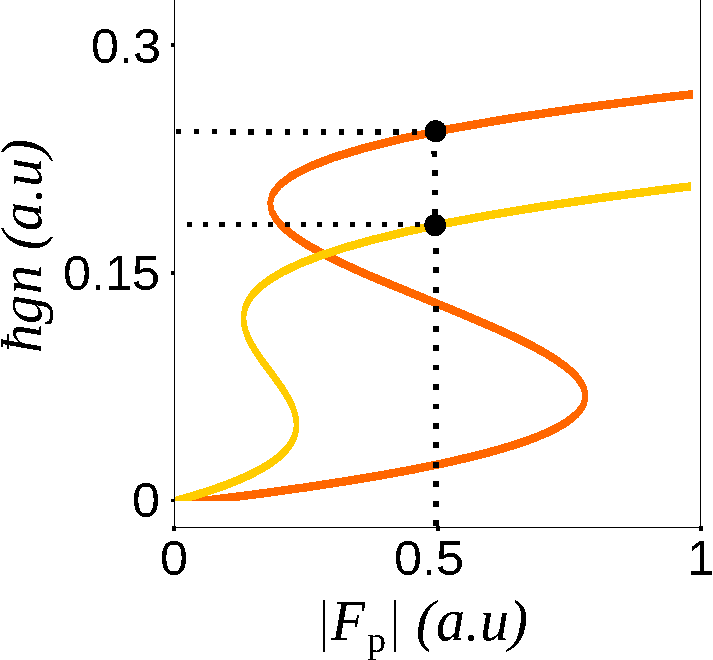
\includegraphics[width=0.4\textwidth]{chap_custom_st/fig/bistab_to_gn.pdf}
    \caption{Bistability cycle for two different values of the effective detuning $\delta(k^{(1)}_p)$ (yellow) $\leq \delta(k^{(2)}_p) $ (orange) when $k^{(2)}_p \leq k^{(1)}_p $. The vertical dashed line
    represent the input intensity of the pump laser whereas the black dots represent the operating points of the system for each detuning. The region with the higher wavevector
    yields a lower $gn$ value.}
    \label{fig:bistab_steep}
\end{figure}

Here we exploit the phenomenology and implement the target profile \autoref{eq:target_velocity} with a large difference between $v_\mathrm{d}$ and $v_\mathrm{u}$, a transition width $w_\mathrm{H}=\SI{20}{\micro\meter}$ and a detuning $\delta(0)=\SI{71}{\giga\hertz} \rightarrow\hbar\delta(0)=\SI{0.3}{\milli \electronvolt}$
\autoref{fig:bh_steep} (b) shows $v_0(x)$ (solid lines) as well as $c_\mathrm{s}(x)$ (dot-dashed lines). The two supercritical fluids created in the smooth configuration 
have an horizon steepness $\kappa$ of $\SI{0.07}{\per \pico \second}$ (red) and $\SI{0.08}{\per \pico \second}$ (purple) whereas in the steep geometry implemented here we compute $\kappa = \SI{0.11}{\per \pico \second}$. The excitation spectra are shown in \autoref{fig:bh_steep} \textbf{c)} and \textbf{d)}.
The frequency range at which paired emission is possible is roughly the same than in the smooth case \textbf{f)} $\Delta \omega_H$= 28 GHz whereas the horizon steepness 
gets increased by 25\%. This independent tuning of $\kappa$ and the paired emission spectrum is not possible in conservative quantum fluids such as atomic BECs, for example.
The fine control over the waterfall horizon geometry we demonstrate here is interesting to test recent tunneling models for the Hawking effect~\cite{delporro2024tunneling}.


\begin{figure}
    \centering
    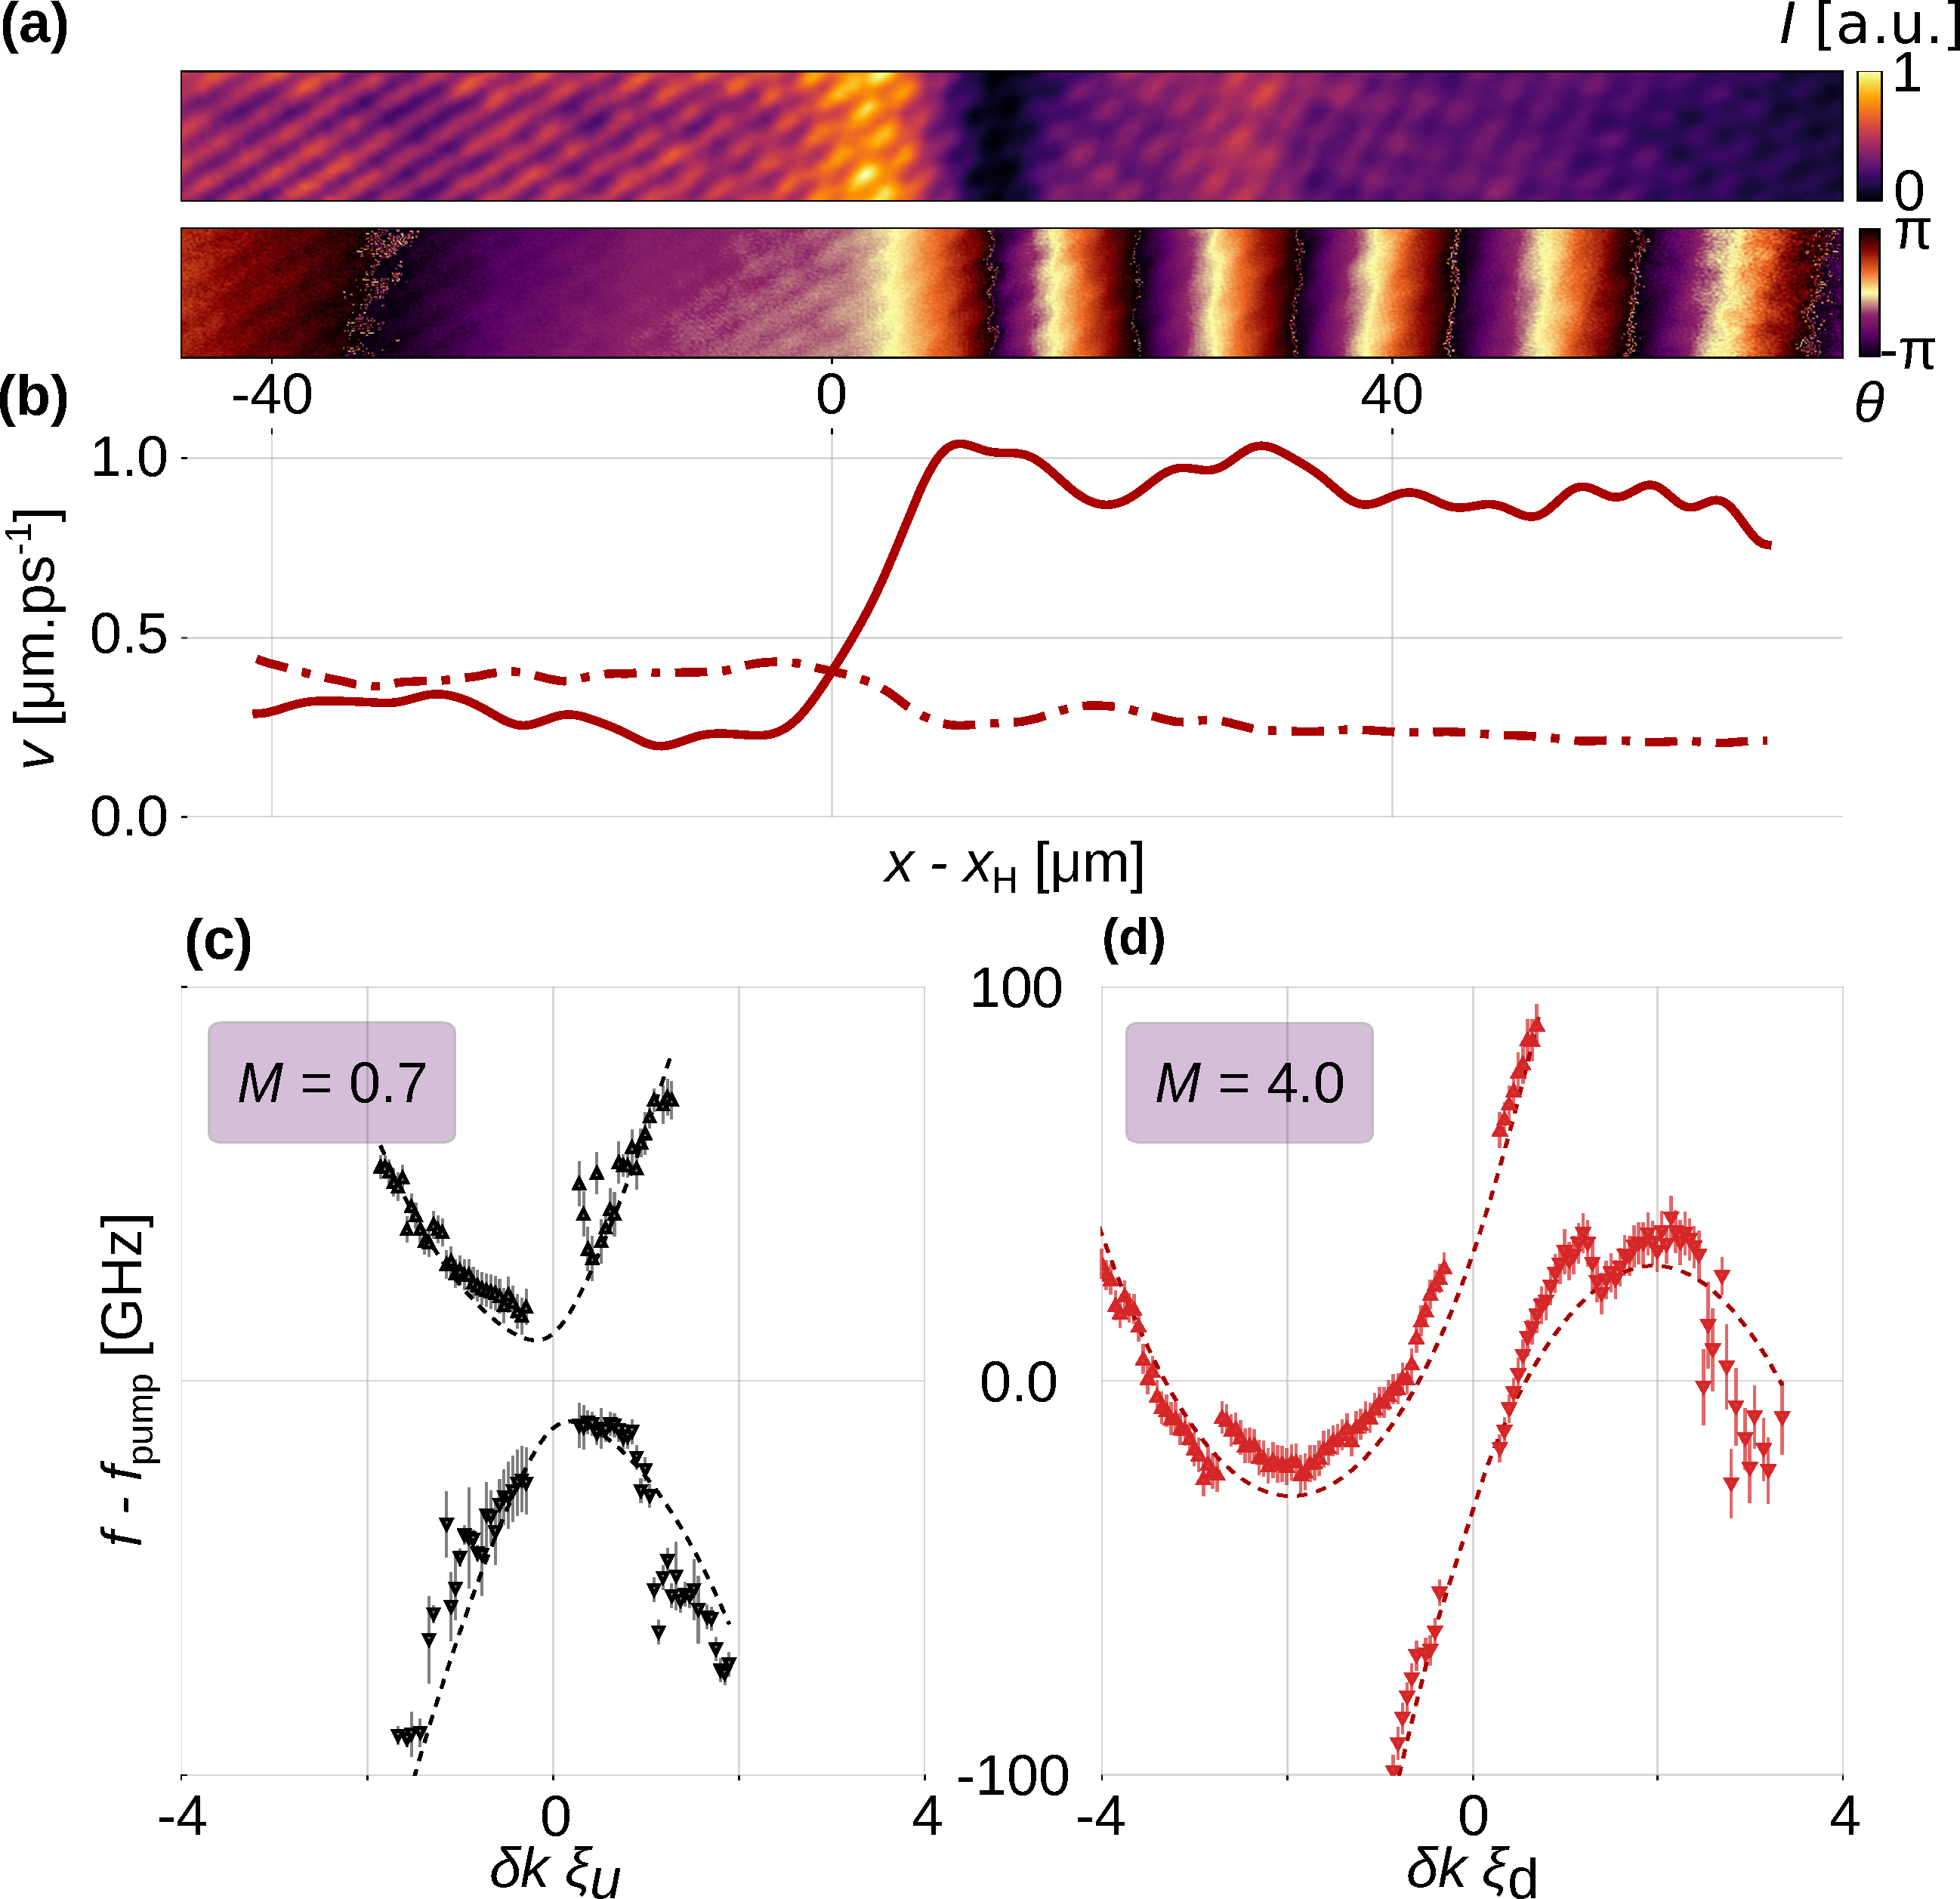
\includegraphics[width=0.7\textwidth]{chap_custom_st/fig/bh_steep.pdf}
    \caption{\textbf{Steep horizon}.    
    \textbf{(a)} Measured fluid density (top) and phase (bottom).
    \textbf{(b)} Measured fluid velocity profile.
    Solid line, $v_0(x)$; dashed line, $c_\mathrm{s}(x)$.
    \textbf{Excitation spectra} Eq.~\eqref{eq:lfbogo}: \textbf{(c)} upstream region. \textbf{(d)} downstream region; dashed lines, fit with free parameter $gn$. Error bars represent the uncertainty in the determination
    of the center of the lorentzian when each scan is fitted by a lorentzian function to find the resonance energy. The $M$ values in the inset of each spectrum is the computed Mach number in the corresponding region. }
    \label{fig:bh_steep}
\end{figure}

\subsection{Quasi-normal mode configuration}

The target velocity profile \autoref{eq:target_velocity} can be complexified to create complex horizon geometry by imprinting 
a velocity peak in the transition region. More precisely, we define the \textit{Quasi-Normal Mode} (QNM) target velocity profile as :

\begin{figure}
    \centering
    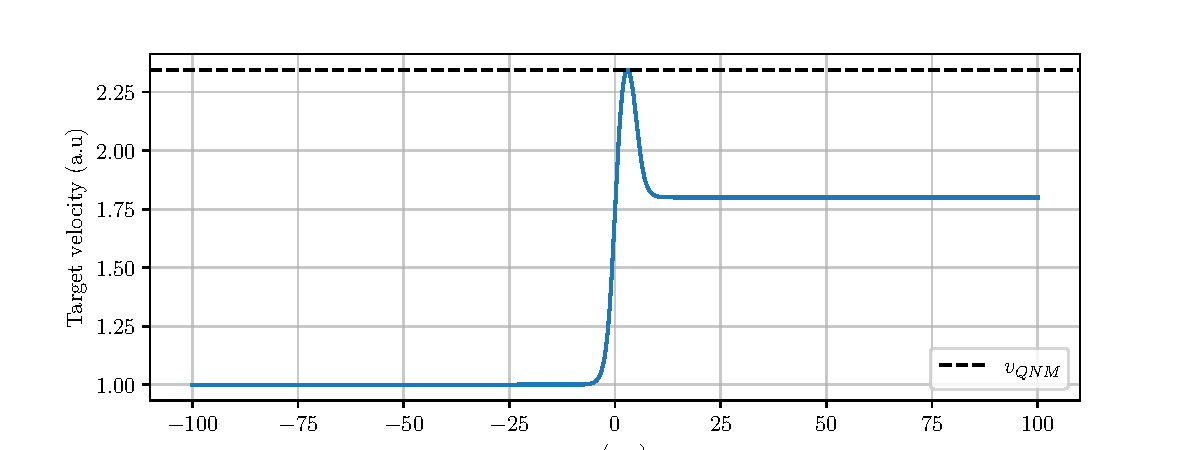
\includegraphics[width=1\textwidth]{chap_custom_st/fig/qnm_target_velocity.pdf}
    \caption{Typical QNM target velocity profile.}
    \label{fig:qnm_target_velocity}
\end{figure}


\begin{equation}
    v(x)= \frac{v_{QNM}-v_{up}}{2}\mathrm{tanh}(\frac{x-x_1}{w_1})+ \frac{v_{d}-v_{QNM}}{2}\mathrm{tanh}(\frac{x-x_2}{w_2})+\frac{v_{up}+v_{d}}{2}
    \label{eq:target_velocity_qnm}
\end{equation}

where $v_{QNM}$ is the velocity of the peak, $v_{up}$ and $v_{d}$ are the upstream and downstream velocities, $x_1$ and $x_2$ are the position of the first and second transition and $w_1$ and $w_2$ are their width.
The typical corresponding shape is shown in \autoref{fig:qnm_target_velocity}.
With the same asymptotic parameters as in the smooth horizon configuration of \autoref{fig:smooth_transition} \textbf{e)} we create a fluid with the QNM target velocity profile.
\begin{figure}
    \centering
    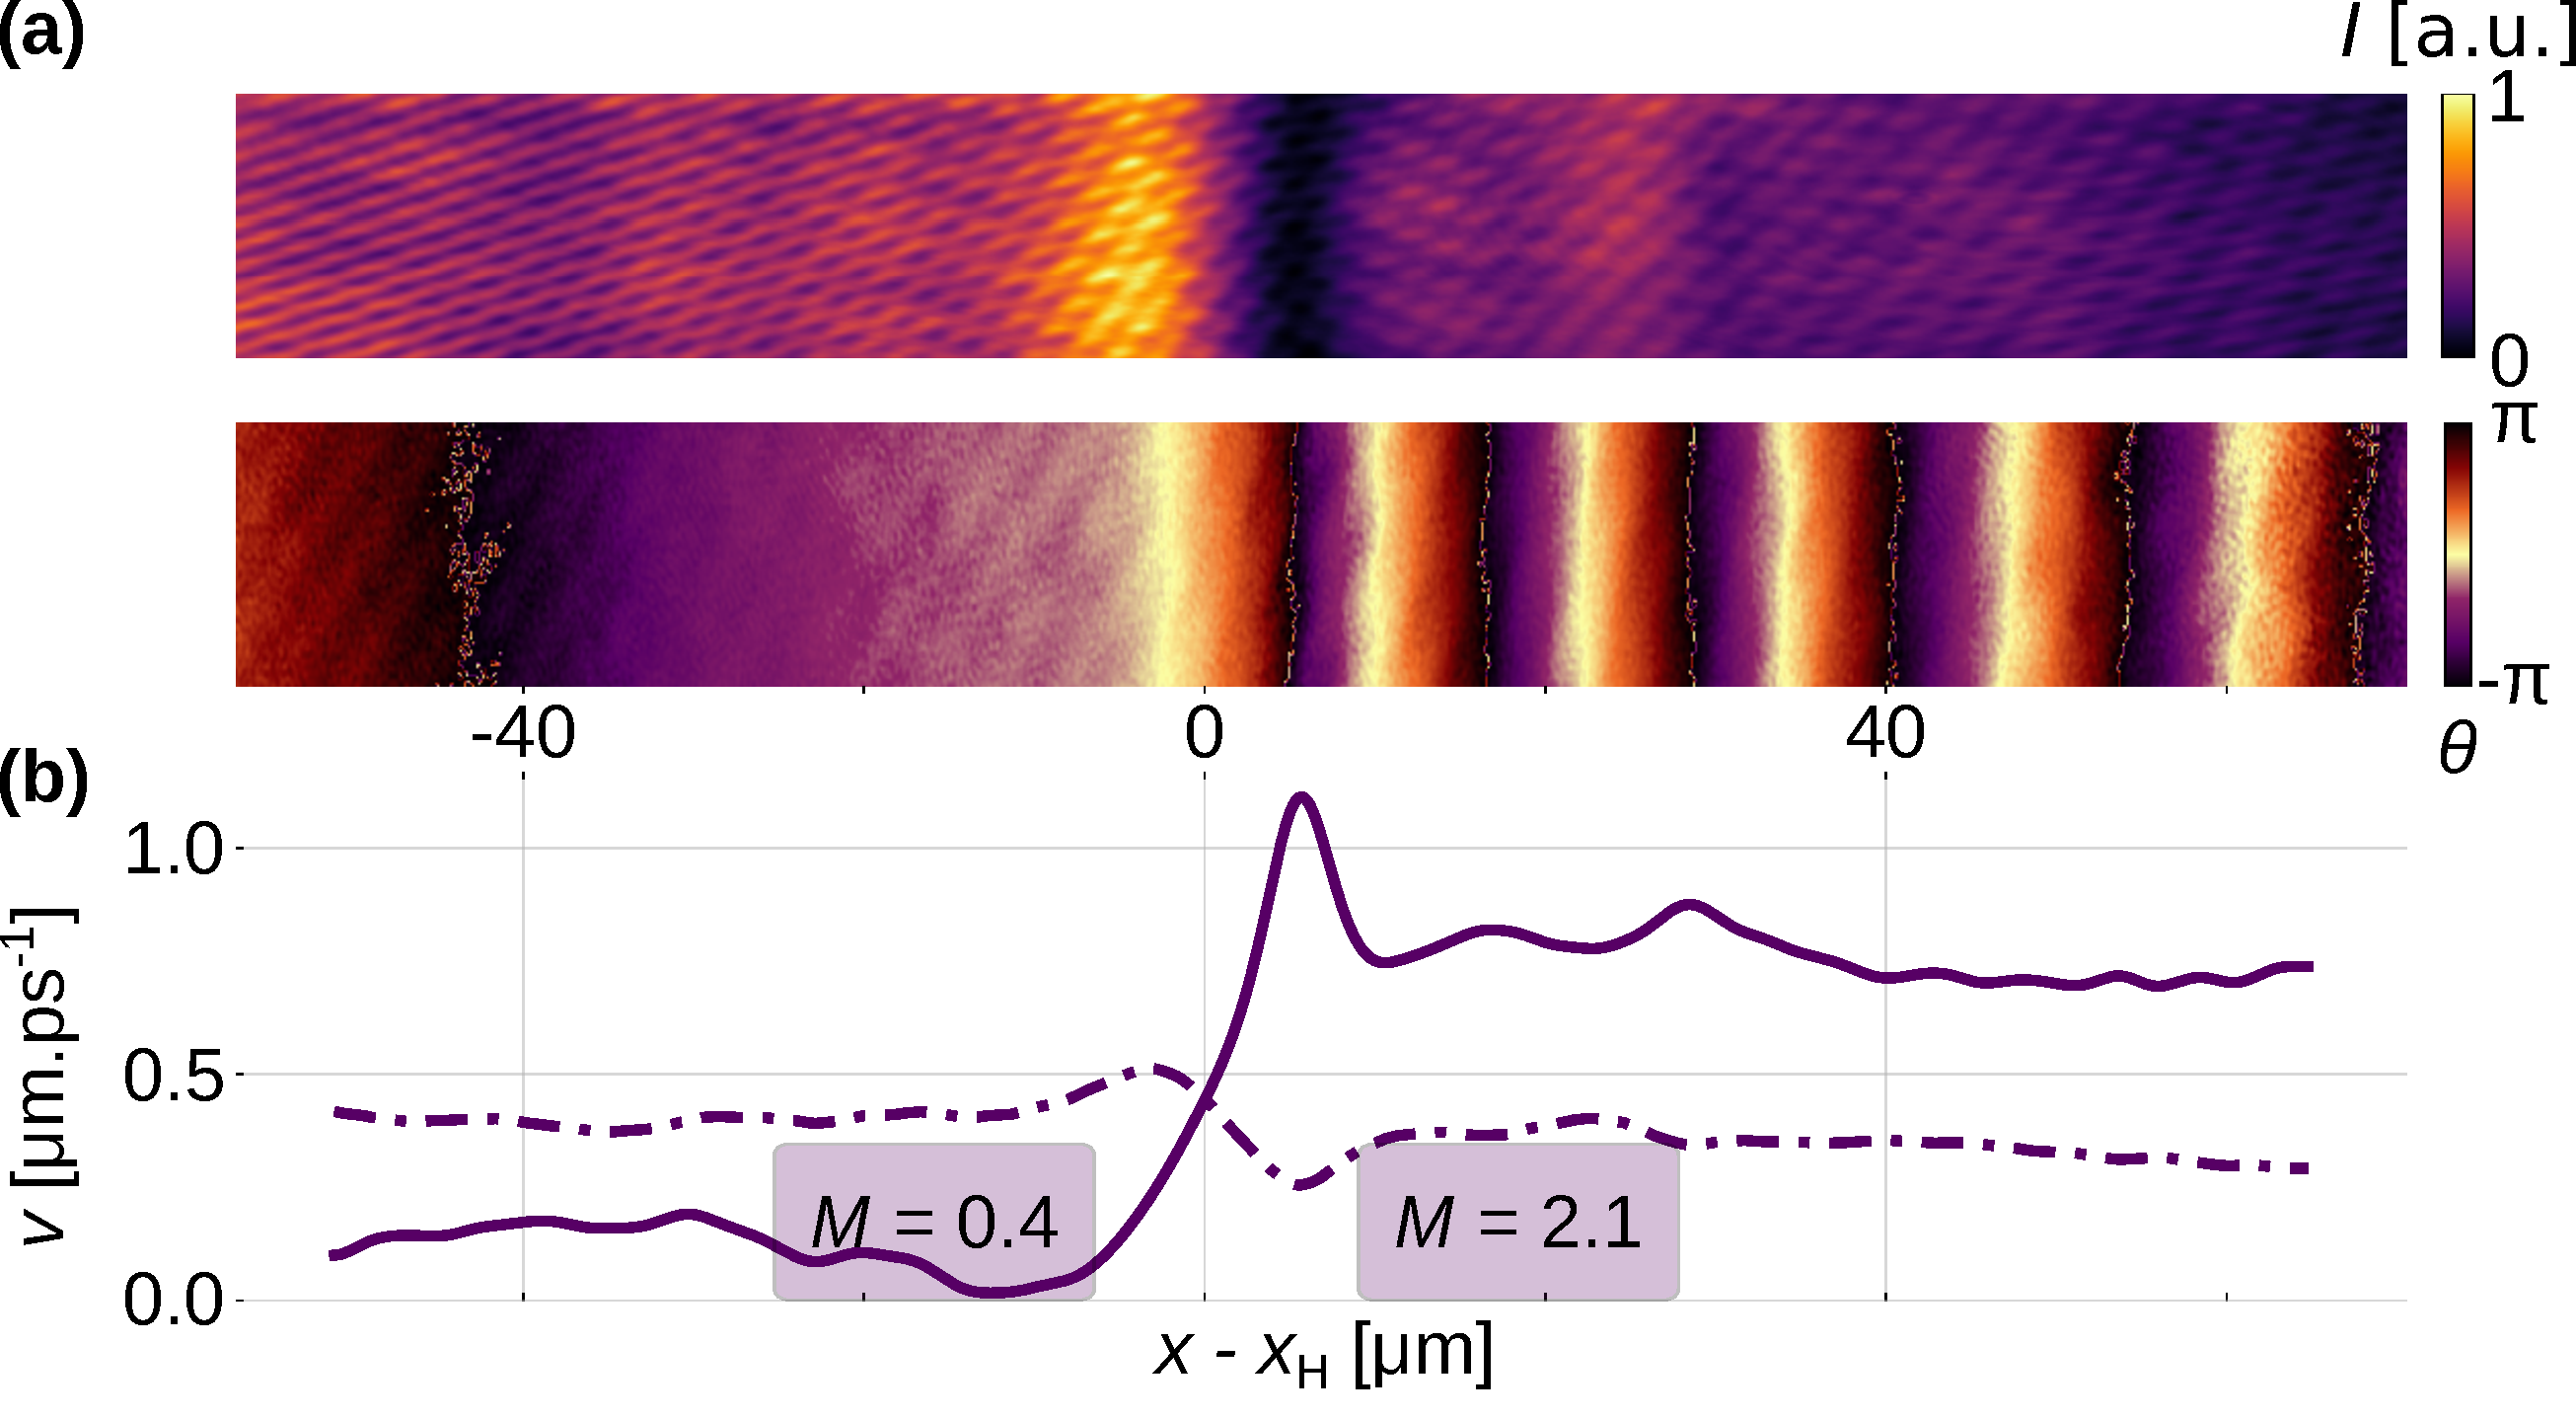
\includegraphics[width=0.7\textwidth]{chap_custom_st/fig/bh_qnm.pdf}
    \caption{\textbf{Quasi-normal mode horizon}.    
    \textbf{(a)} Measured fluid density (top) and phase (bottom).
    \textbf{(b)} Measured fluid velocity profile.
    Solid line, $v_0(x)$; dashed line, $c_\mathrm{s}(x)$.}
    \label{fig:bh_qnm}
\end{figure}

First, the asymptotic velocities are as expected, not modified by the presence of the peak, while the surface gravity 
is greatly enhanced as $\kappa = \SI{0.19}{\per \pico \second}$, almost twice the value obtained in the steep configuration.
But the most peculiar feature of the QNM configuration is the density dip that comes with the velocity peak. For the reason explained in the previous section,
the velocity peak imprinted here is associated with a density dip. As the dip is surrounded by two regions of higher density, it forms an effective resonator for bogoliubov excitation.
This leads to the appearance of a metastable excitation mode of $\phi$ called a quasi-normal mode: here specifically, a negative-energy standing wave can establish itself inside the resonator (at $\omega_\mathrm{QNM}>\mathrm{max}(\omega_\mathrm{B}^-|_{x>x_\mathrm{H}})$) and tunnel-couple with positive-energy propagating waves on either side \cite{jacquet_quantum_2023}.
This quasi-normal mode is spontaneously excited by quantum vacuum fluctuations of $\phi$.
As a result, the Hawking spectrum is predicted to peak at the frequency of the quasi-normal mode, bearing signatures of the near-horizon geometry. 
In some sense, the QNM configuration is a quantum analogue of the black hole ringdown phase, where the black hole emits gravitational waves with a characteristic frequency and damping time \cite{brito_gravitational_2015} that depend on its parameters. 


\section{Conclusion}

We demonstrated full optical generation and characteziation of mean field with arbitrary velocity profiles in a polariton fluid which act as effectivly curved spacetime for 
bogoliubov excitation. In each
configuration, we were able to measure the collective excitation spectrum of the fluid and state or not if Hawking radiation could be observed. We showed that the critical velocity to observe negative energy modes is not necessarly the speed of sound but rather a critical velocity 
that depends on the fluid parameters. This widens the range of experimental configurations at which particle creation can be observed. The great versatility of our experimental methods also showed that the steepness of the horizon can be controlled independently of the paired emission spectrum.
Finally, we demonstrated the possibility to create complex horizon geometry that could yield peculiar behaviors like Quasi Normal Modes. The great 
advantage of the system presented here is the great range of field theory scenario that can be tested in a single setup. Eventhough
 trans-critical polariton fluids are far from encapsulating what truly happen at a black hole horizon, its a great platform to study effect predicted by field theory in curved spacetime, regardless they were
originally thought for black holes or not.

\subsection{Outlook}

% !TeX encoding = UTF-8
% !TeX spellcheck = fr_FR
% !TeX root = ../mythesis.tex
% !TeX program = pdflatex (build)
%%% TeXmaker : no 'magic comments' but set Root with Options > Set as master file
\graphicspath{{./}{./fig/}{./chap_stimulated_hawking/fig/}}

\chapter{Experimental observation of stimulated Hawking radiation in a polariton quantum fluid}
\label{chap:stimulated_hawking}



In the previous chapter, we demonstrated the experimental realization of a transcritical flow in a polariton quantum fluid through precise optical pump shaping. This allowed us to engineer the fluid's density and velocity profiles to form a transcritical region, a key ingredient for the emergence of a sonic horizon. Furthermore, we presented experimental evidence of negative-energy modes in this region, confirming the necessary conditions for the observation of the Hawking effect.

Building on these achievements, this chapter focuses on the experimental observation of stimulated Hawking radiation in a polariton fluid. Stimulated emission provides a controlled way to probe the Hawking effect by injecting a coherent state into the upstream region and measuring its scattering into outgoing modes. This approach allows us to directly study the amplification of positive-energy modes and the role of negative-energy modes in the transcritical region.
The experimental realization of stimulated Hawking radiation involves several key steps. First, we describe the setup used to inject coherent states into the polariton fluid and the techniques employed to measure the outgoing modes. 
Next, we introduce a method to analyze the scattered modes. Although the scattering matrix is not directly measured, this approach reveals clear signatures of amplification, providing indirect evidence of the underlying scattering process.
 Finally, we present the results of these measurements, discuss the agreement with theoretical predictions and the robustness of the stimulated Hawking effect.
The results presented in this chapter not only validate the theoretical predictions of stimulated emission but also establish a pathway toward the observation of spontaneous Hawking radiation. By leveraging the unique properties of polariton fluids, this work demonstrates the potential of these systems as a platform for exploring fundamental aspects of quantum field theory in curved spacetime and beyond.


\begin{figure}[htbp]
    \centering
    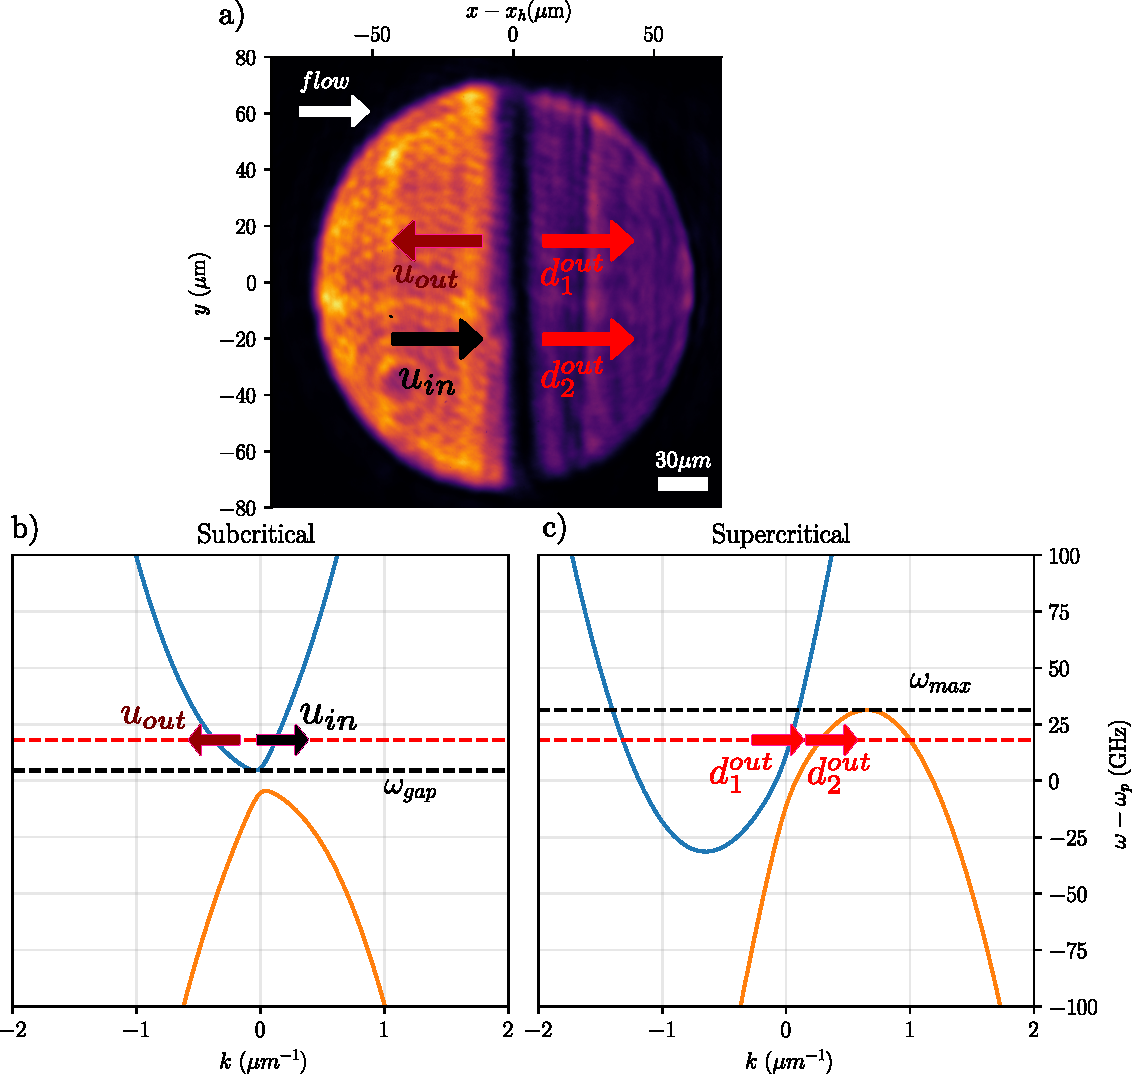
\includegraphics[width=1\textwidth]{chap_stimulated_hawking/fig/typical_dens_2D.pdf}
    \caption{\textbf{a)} Real space image of a transcritical flow of polaritons with detuning $\delta(0)=29 GHz$ and wavevectors $k_u=0.1 \mu m^{-1}$ and $k_d=0.6\mu m^{-1}$. The black arrow represents the impinging mode $u_{in}$ while the red arrows represent the outgoing modes $u_{out}$, $d_1^{out}$ and $d_2^{out}$. The direction
    of the arrow reflects the sign of the group velocity of each mode.
    \textbf{b)} Typical analytical Bogoliubov dispersion relation in the upstream subcritical region. The arrows correspond to the modes displayed on the left side of \textbf{a)}. 
    \textbf{c)} Typical analytical Bogoliubov dispersion relation in the downstream supercritical region. The arrows correspond to the modes displayed on the right side of \textbf{a)}}
    \label{fig:typical_dens_2D}
\end{figure}


\section{Interferometric measurement of the scattering matrix }
\label{sec:principle_measurement}

We aim at solving the scattering problem of a coherent state injected in the upstream region impinging on the horizon.
This approach is complementary to what has already been done in the hydrodynamical experiment \cite{euve_scattering_2020} in which
the stimulating field came from the transcritical region.

\subsection{Challenges of the measurement}


Let us take a transcritical flow of polaritons with a typical density profile shown in \autoref{fig:typical_dens_2D} \textbf{a)}. The bright
region on the left corresponds to the upstream subcritical region, while the other side of the interface is the transcritical region. Typical analytical spectra corresponding to each region are shown in \textbf{b)} and \textbf{c)}.
The previous chapter evidenced that it is possible to locally excite the Bogoliubov dispersion by shining a weak probe laser at the right couple of parameters $(\omega, k)$. Consider then a coherent state
$\ket{\alpha_{in}}$ in the $u_{in}$ mode of \textbf{b)} that is, an upstream mode that impinges on the interface. If its frequency $\omega_{in}$ is within $[\omega_{gap}, \omega_{max}]$ we expect to measure one reflected mode $u_{out}$ and two transmitted modes $d_1^{out}$ and $d_2^{out}$. The latter is the negative
energy mode responsible for Hawking radiation. Each of these modes has a different wavevector $k_i$.

\bigskip


Experimentally, this situation corresponds to four distinct optical signals exiting the sample at different angles, or equivalently, to four spatially separated spots in the Fourier plane of the cavity. To illustrate the inherent challenges associated with such measurements, we present in \autoref{fig:bh_k_space} \textbf{b)} the typical expected locations of the scattered signals in the Fourier plane corresponding to the fluid configuration of \autoref{fig:typical_dens_2D} \textbf{a)}. The two bright spots correspond to the regions of the fluid characterized by the wavevectors \(k_u\) and \(k_d\). 

First, the expected position of the mode \(d_1^{\text{out}}\) nearly coincides with the pump signal in the downstream region. Since the probe intensity must remain at least two orders of magnitude lower than that of the pump to preserve the perturbative regime, the resulting signal-to-noise ratio is extremely low. Consequently, a direct measurement of the \(d_1^{\text{out}}\) at wavevectors close to that of the pump mode becomes unfeasible.

Second, in addition to the desired signals at frequency \(\omega_{\text{in}}\), all modes are subject to four-wave mixing processes due to nonlinear interactions with the pumped polaritons. As a result, depending on the fluid parameters, the conjugate modes generated by these interactions may spatially overlap with the reflected or transmitted modes. For example, as illustrated in \autoref{fig:bh_k_space}, the conjugate of the injected mode \(u_{\text{in}}\) appears at the same location in momentum space as the reflected mode \(u_{\text{out}}\). Consequently, prevents a clear distinction between the two contributions.

The central challenge of this measurement is thus to detect weak signals on top of a strong background while ensuring that these signals originate from genuine transmission and reflection at the interface --rather than from spurious scattering events or nonlinear mixing. Therefore, the critical experimental objective is to optimize the signal-to-noise ratio, where “noise” refers to all undesired signals. This is achieved by acting on two main experimental parameters:


\begin{figure}
    \centering
    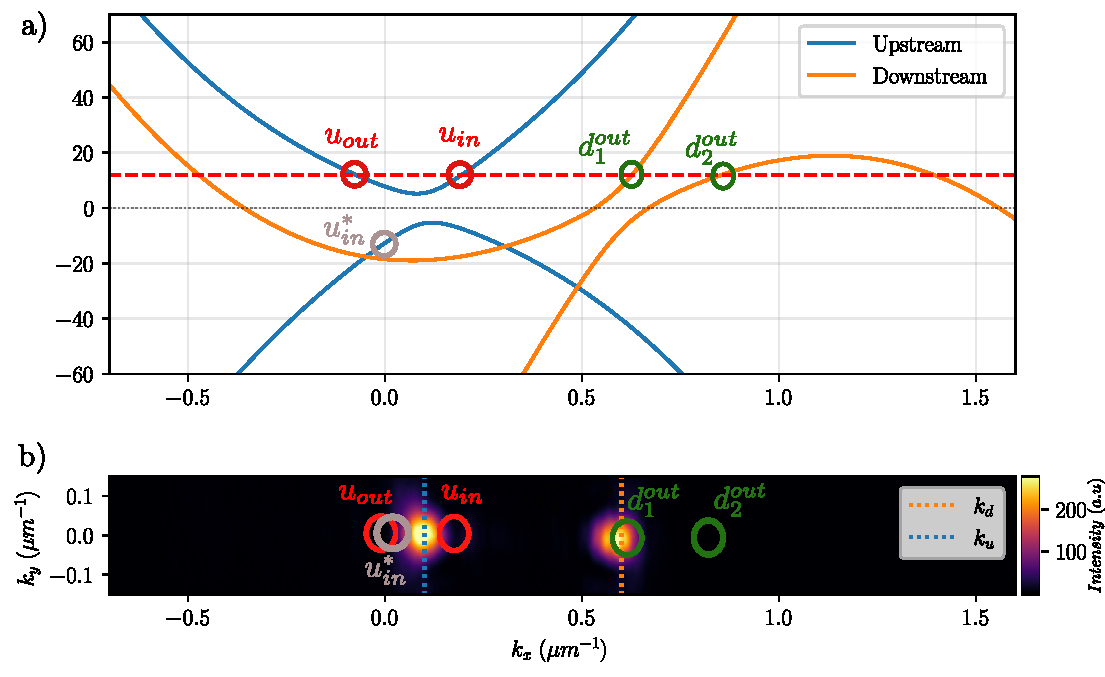
\includegraphics[width=1\textwidth]{chap_stimulated_hawking/fig/bh_k_space.pdf}
    \caption{\textbf{a)} Analytical Bogoliubov dispersion of both regions calculated with the parameters of the fluid of \autoref{fig:typical_dens_2D} \textbf{a)}. To show what happens in practice, the two dispersions are plotted in the same graph as a function of the wavevector in the laboratory frame. The upstream dispersion
    is centered at $k_u=\SI{0.1}{\per \micro \meter}$ while the downstream one is centered at $k_d=\SI{0.6}{\per \micro\meter}$. The red dashed line corresponds to the energy of the injected mode. The wavevectors of the reflected-transmitted represented by the vertical dashed lines modes are obtained 
    at the intersections of this line with the Bogoliubov branches and reported in the momentum space \textbf{b)}. The red (resp. green) circle represents the expected location 
    of the upstream (resp. downstream) modes. Finally, the grey circle represents the conjugate of the injected signal resulting from four-wave mixing. \textbf{b)} Momentum space of \autoref{fig:typical_dens_2D} \textbf{a)}: the two bright spots correspond to the two regions of the fluid with wavevectors $k_u$ and $k_d$. The colored circle
    correspond to the reflected and transmitted modes shown in \textbf{a)}.}
    \label{fig:bh_k_space}
\end{figure}

\begin{itemize}
    \item \textbf{Enhancement of the signal}: As discussed in the previous chapter, this can be accomplished by increasing the steepness of the horizon.
    \item \textbf{Suppression of the pump background}: The photonic nature of the system allows us to exploit two key properties of light: polarization and coherence. Polarization filtering can be applied in the detection path, while coherence enables the use of interferometric techniques, as will be detailed in the following section.
\end{itemize}

\textbf{Electronic filtering.} One possible strategy to suppress the pump background is inspired by the method used to measure the excitation spectrum in the previous chapter. By modulating the intensity of the probe beam at a frequency \(\omega_{\text{mod}}\) accessible in the electronic domain, the signal can later be demodulated, isolating the component arising from the probe-induced excitation. However, in the current context, what previously served as an advantage becomes a limitation. Indeed, the four-wave mixing signals also carry the modulation, thus failing to resolve overlapped modes as explained above. To overcome this, we turn to the optical domain, specifically to interference-based detection schemes.

\subsection{Interferometric reconstruction of the scattered field}

The measurement is based on the same interferometric technique previously employed to reconstruct the mean field.
 The key distinction here is that the method is now applied to the probe field instead. Although this adjustment is minor in practice, it represents a significant conceptual shift that enables a comprehensive characterization of the scattering problem. 
Before detailing its experimental implementation in the context of the scattering problem, we first examine the insights that such a measurement can provide.

\bigskip

We again consider the generic situation presented above, namely, a coherent state injected in the upstream region. The full optical field transmitted through
the sample is composed of :

\begin{itemize}
    \item The mean field $\psi_0$ oscillating at the pump frequency $\omega_p$
    \item The probe field oscillating at the probe frequency $\omega_p+\omega_{in}$ resulting from the scattering of $u_{in}$ on the interface.
    \item The conjugate field oscillating at the opposite of the probe frequency $\omega_p-\omega_{in}$ resulting from the four-wave mixing of each $\omega_p+\omega_{in}$ mode with the pump. 
\end{itemize}


\begin{figure}
    \centering
    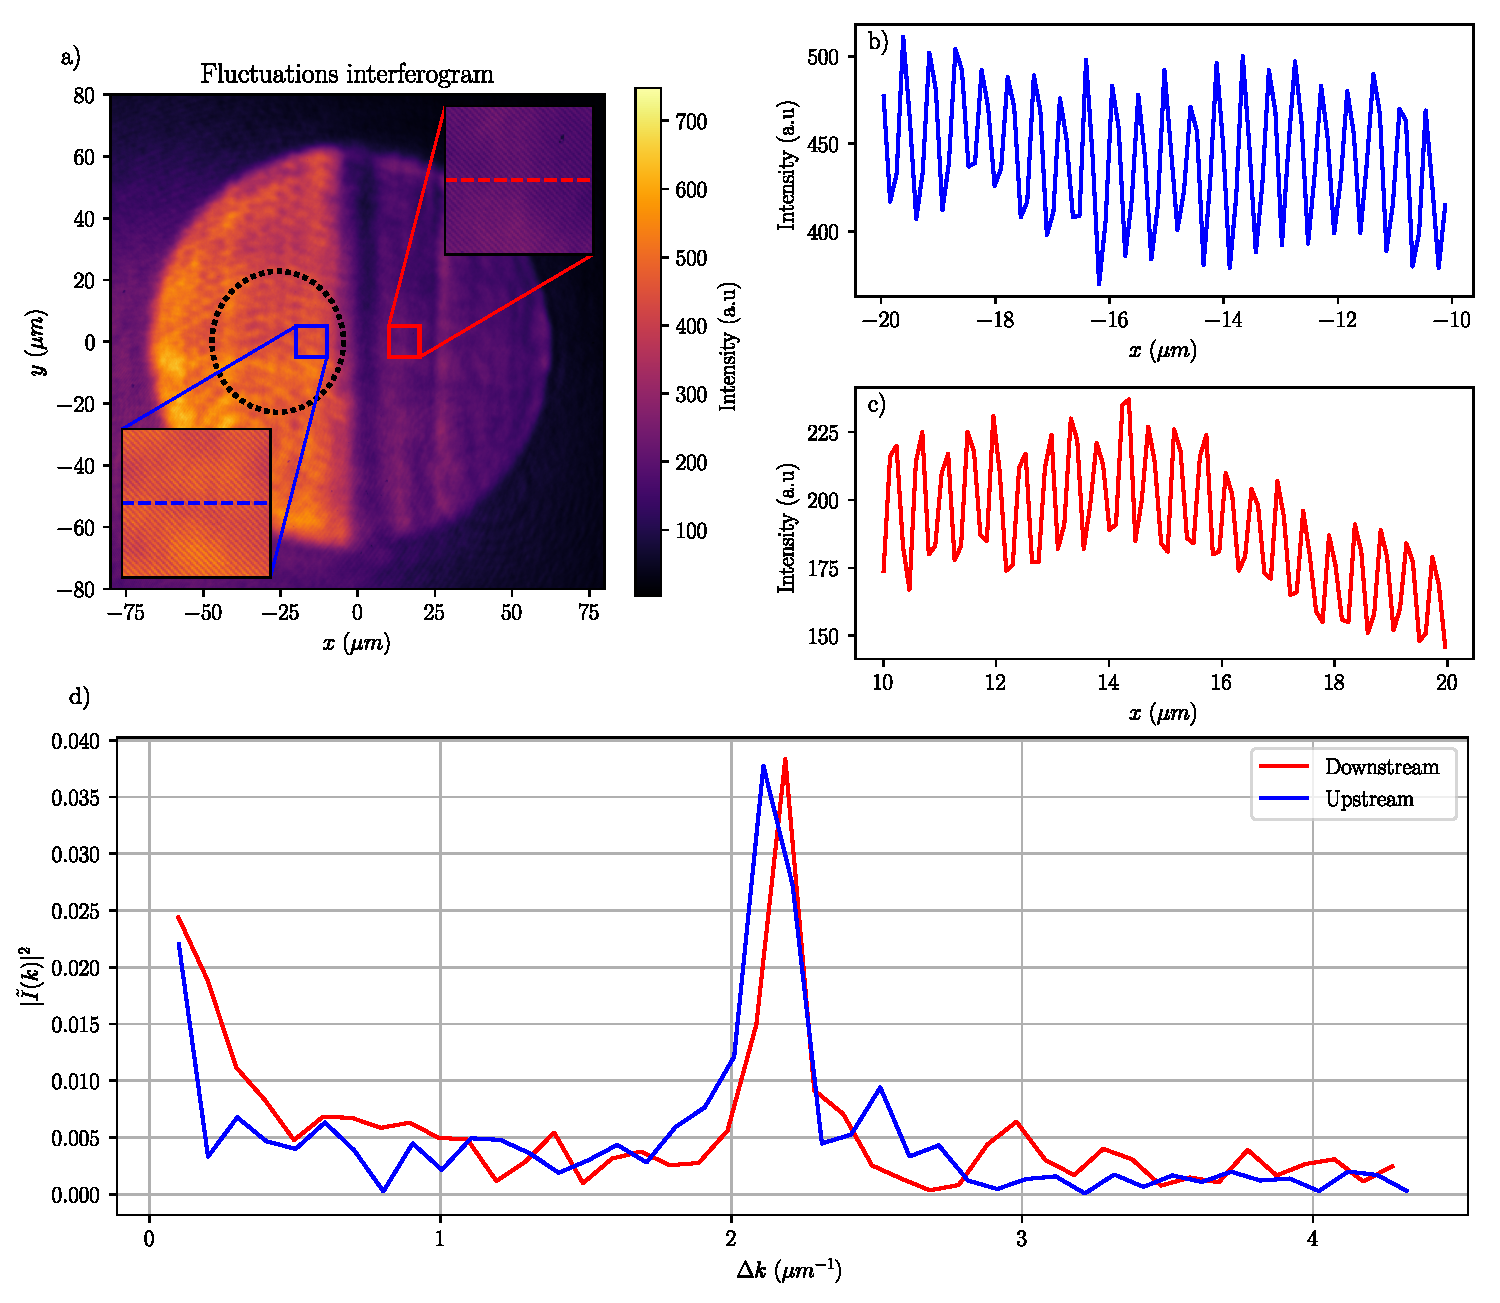
\includegraphics[width=1\textwidth]{chap_stimulated_hawking/fig/interferogram_fluctuations.pdf}
    \caption{\textbf{a)} Interferogram resulting from the superposition of \autoref{fig:typical_dens_2D} \textbf{a)} and a reference beam from the probe laser. The black dashed circle
    represents the injected probe location. The red inset (resp. blue) is a zoom on the upstream (resp. downstream) region near the interface. 
    \textbf{b)} Cut of the interferogram along the red dashed line of the red inset. 
    \textbf{c)} Cut of the interferogram along the blue dashed line of the blue inset. 
    \textbf{d)} Fourier transforms of the cuts \textbf{b)} and \textbf{c)}. The blue curve corresponds to the upstream region with spatial frequency $\Delta k_u\approx\SI{2.11}{\per \micro \meter}$. The red curve corresponds to the downstream region with spatial frequency $\Delta k_d= \SI{2.19}{\per \micro \meter}$. 
     }
    \label{fig:interferogram_fluctuation}
\end{figure}
In what follows, we work in the pump rotating frame, whereby all frequencies are measured relative to $\omega_p$.
When the probe field is superimposed with a phase reference beam at the probe frequency—obtained as a pick-off from the probe laser—the only components that generate interference fringes are those oscillating at \(+\omega_{\text{in}}\). 
Each scattered mode is characterized by a distinct wavevector \(k_i\), leading to a unique spatial frequency in the resulting interferogram.
As an illustrative example, \autoref{fig:interferogram_fluctuation}~\textbf{a)} displays two regions of such an interferogram.
 The first one lies within the probe injection area, where the fringe spacing is inversely proportional to \(\abs{\Delta k}\), with \(\Delta k = k_{u_{\text{in}}} - k_{\text{ref}}\) denoting the wavevector mismatch between the injected mode and the reference beam. 
 The second region is located downstream, beyond the probe injection area. The mere presence of interference fringes in this region already confirms that the injected mode has propagated through the interface, while the fringe spacing provides direct information about the wavevector of the transmitted mode.

To clarify this, we perform the spatial Fourier transforms of the two regions and show the result in \autoref{fig:interferogram_fluctuation}~\textbf{d)}. The signal near \(\Delta k=0\) corresponds to the continuous background signal—primarily the pump field and the conjugate modes at \(-\omega_{\text{in}}\)—which do not interfere with the reference beam. It is the analog of the DC signal in electronics. The central peaks represent the spatial frequencies of the propagating components in each region. Notably, the downstream region exhibits a higher wavevector, consistent with the scattering picture.

This preliminary analysis already highlights the strength of the technique. By applying numerical masks at different spatial locations, one can selectively extract the Fourier components of the fluctuations. More generally, a single interferogram enables a full reconstruction of the probe field at the frequency of the injected perturbation. As a result, this method proves particularly well-suited for addressing the scattering problem, as it overcomes all the challenges previously outlined :



\begin{itemize}
    \item Conjugate modes and background contributions from the pump are inherently filtered out, as they do not interfere with the reference beam and therefore do not generate fringes.
    \item Each scattered mode gives rise to a distinct spatial frequency in the interferogram, enabling their individual identification and selective extraction.
    \item The interference with the coherent reference beam enhances the signal-to-noise ratio, thereby facilitating the detection of weak scattered components.
\end{itemize}


The interferometric technique outlined above provides a powerful framework for reconstructing the probe field and isolating the scattered modes.
 By leveraging the distinct spatial frequencies of the scattered components and filtering out unwanted contributions, this method enables a precise characterization of the scattering process. In the following section, we detail the experimental implementation of this approach, focusing on the setup and procedures required to reconstruct the scattering matrix and extract the key parameters governing the stimulated Hawking effect.

 \section{Experimental implementation}
 The experiment is conducted in the same microcavity as in the previous chapter, operating at the same working point (C5-D6) and using an identical optical setup. 
 However, whereas the previous measurements focused on characterizing the fluid's excitation spectrum, the present objective is to detect the scattered signals generated at the horizon interface. 
 To this end, we first investigate configurations in which the horizon is as sharp as possible, even at the cost of significantly reducing the downstream density. 
\label{sec:exp_implementation_scat_matrix}
\subsection{Ballistic configuration}
\label{sec:ballistic_configuration}
This is accomplished by illuminating only the upstream region with the pump laser, set at a wavevector \(k_p = \SI{0.02}{\per \micro \meter}\). As a result, the downstream region consists of polaritons propagating ballistically beyond the pumped area.
The pump is detuned by \(\delta(0) = \SI{26}{\giga \hertz}\) in order to reach the high-density regime of optical bistability. Additionally, the Gaussian intensity profile of the pump beam is truncated into a half-disk shape with a diameter of \(\SI{150}{\micro \meter}\), thereby generating a sharp intensity gradient at the edge of the pumped region. 
The resulting mean-field profile is presented in \autoref{fig:bh_density}.

\begin{figure}[htbp]
    \centering
    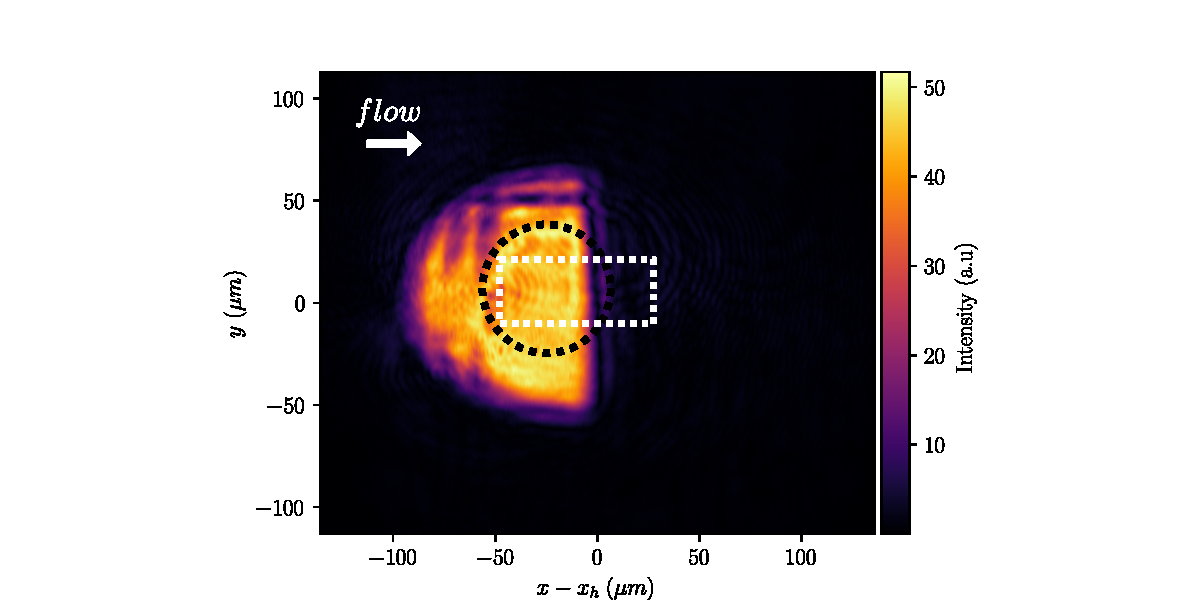
\includegraphics[width=1\textwidth]{chap_stimulated_hawking/fig/bh_density.pdf}
    \caption{\textbf{a)} Real space image of a transcritical flow of polaritons with detuning $\delta(0)=\SI{48}{\giga\hertz}$. The pump is shone only 
    in the upstream region with wavevector $k_p=\SI{0.02}{\per \micro \meter}$.
    The downstream region is made of polaritons propagating ballistically. The black dashed circle represents the location of the injected probe while the white dashed rectangle represents the region 
    of interest (ROI) for the density and velocity profiles. }
    \label{fig:bh_density}
\end{figure}

As shown on the corresponding intensity and velocity profiles [see \autoref{fig:bh_balistic}~\textbf{a)}], the downstream region exhibits an exponentially decaying density accompanied by an increasing flow velocity. 
This behavior naturally arises from the conservation of current, as described by the continuity equation ~\ref{eq:continuity}, in the absence of external pumping. More precisely, it can be shown that 
away from the pump spot in a slowly varying region where the quantum pressure can be neglected, the Gross Pitaevskii equation takes the form of a generalized Bernoulli equation for driven dissipative fluids. The wavefunction then takes the form \cite{carusotto_inhomogeneous_2008}: 

\begin{equation}
    \psi_0(x \gg x_h) = \sqrt{n_0}e^{-\frac{x}{l_d}}e^{i k_{fluid}x},
\end{equation}
where $1/l_d=\gamlp/2v_g$ is the spatial decaying rate resulting from the product between the fluid group velocity $v_g =\hbar k_{fluid}/\mlp $ and the polariton lifetime $1/\gamlp$. The local wavevector of the polariton fluid $k_{fluid}$ is determined by the equation: 
\begin{equation} 
    \omp = \omlp + \frac{\hbar k_{fluid}^2}{2m} + gn_0(x) + g_r n_r(x).
    \label{eq:bernoulli}
\end{equation}
Taking the low density limit $gn_0, g_rn_r \to 0$, the asymptotic value of $k_{fluid}$ is fixed by the detuning $\delta(0)$ in the pumped region as $k_d \coloneqq k_{fluid}(x \gg x_h) = \sqrt{2m\delta(0)}/\hbar$.
This evolution can also be understood through the optical properties of the system : photons propagating from the pumped region encounter a zone of lower polariton density, which corresponds to a higher effective refractive index. According to Snell-Descartes laws of refraction, the wavevectors of the photons are bent toward the normal of the interface, effectively resulting in an increase in the group velocity. 
The corresponding velocity profile measured by off-axis interferometry is depicted in \autoref{fig:bh_balistic}~\textbf{b)}.  The horizon then forms
spontaneously due to the simultaneous increase of the flow velocity and the decrease of the speed of sound.

\bigskip


The speed of sound is calibrated with the same method as in \autoref{chap:generation_transonic_fluid} from the Bogoliubov spectrum measurement shown in \autoref{fig:fit_bogo}. The latter allows to obtain the interaction energy $gn_0 =9.6 \pm \SI{0.1}{\giga \hertz}$.
In this configuration, the surface gravity is $\kappa\approx \SI{18}{\per \pico \second}$, which is two order of magnitude higher than what was obtained 
in the steepest horizon of the previous chapter. The price to pay for this enhancement is the appearance of oscillations in the downstream fluid density and velocity profiles as shown in \autoref{fig:bh_balistic}.
Indeed, since the pump is no longer present to fix the phase of the system and inject density, the fluid is more sensitive to fabrication defects in the microcavity, each of them
acting as a scattering center.



\begin{figure}
    \centering
    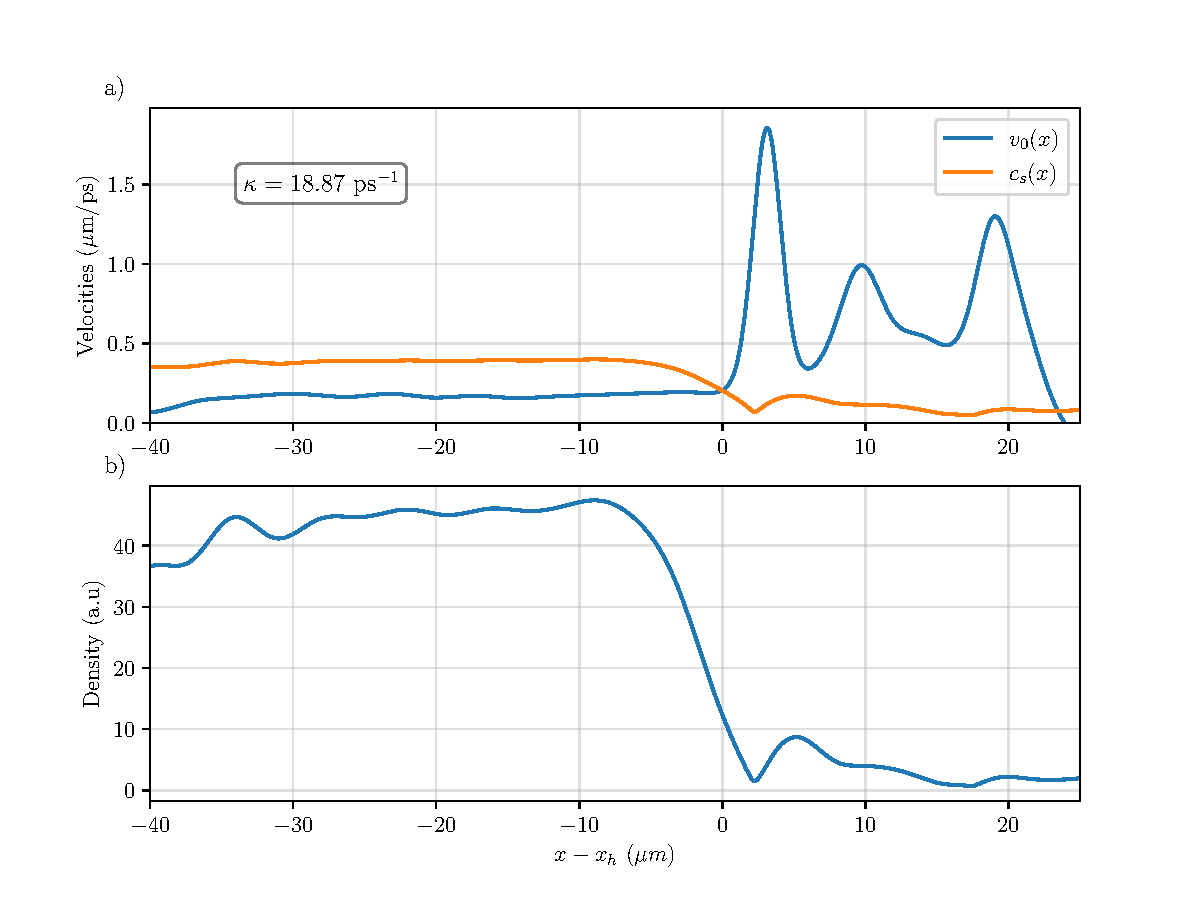
\includegraphics[width=1\textwidth]{chap_stimulated_hawking/fig/bh_balistic.pdf}
    \caption{\textbf{a)} \textbf{Velocity profiles of the fluid in the ROI.} The blue curve corresponds to the velocity of the fluid obtained by off axis interferometry. The orange
    curve corresponds to $c_s=\sqrt{gn_0/\mlp}$ calibrated from the value of $gn_0$ fitted from the upstream Bogoliubov spectrum. \textbf{b) Density profile of the polariton fluid taken in the region of interest.} The profile is obtained by taking an
    average along the $y$-axis on the whole ROI represented by the white dashed rectangle of \autoref{fig:bh_density}. }
    \label{fig:bh_balistic}
\end{figure}

\subsection{Measurement of the Bogoliubov spectrum}

In order to determine whether a detected signal originates from genuine scattering at the interface or from a spurious scattering event, we begin by characterizing the Bogoliubov excitation spectrum of the fluid in each region independently.
This is done by employing a technique mixing the high-resolution pump-probe spectroscopy detailed in the previous chapter and the interferometric technique described in the previous section.

\bigskip

First, the probe beam is centered in the upstream region close to the interface as represented by the black dashed circle in \autoref{fig:bh_density}~\textbf{a)}.
A slight spatial overlap with the downstream region across the interface is voluntarily introduced to have access to the spectrum of both regions on a single frequency scan as we will see later. 
Then, the whole field is superimposed with a collimated phase reference beam originating from the probe laser. The diameter of the reference is set to be three times larger than the diameter of the probe beam in order to have the flattest possible phase front.
 The angle difference between the two beams is set to obtain the best spatial frequency resolution as explained in \autoref{sec:phase_measurement}.


Secondly, the wavevector of the probe beam is tuned from $\SI{-1.0}{\per \micro \meter}$ to $\SI{1.0}{\per \micro \meter}$ by 60 steps of $\Delta k =\SI{0.046}{\per \micro \meter}$.
At each step, the probe frequency is scanned $\pm \SI{65}{\giga \hertz}$ around the pump frequency. The main difference from the previous experiment lies in the detection scheme. In fact, instead of modulating the probe intensity to isolate the signal by electronic filtering, we use the aforementioned interferometric technique. A single frequency scan consists of a series of 80 interferograms recorded on a CCD camera. Then, a full dataset is made of $80\times 60$ interferograms, where each image has $2056\times 2464$ pixels encoded on 16 bits
for the best dynamical range. In principle, the number of frames per scan could be increased by performing a longer energy scan, but this would result in a longer acquisition time. Compared to the $600$ points per energy scan available with the previous technique,
the present procedure then suffers from a lack of frequency resolution. However, frequency resolution turned out not to be a limitation, and this drawback
is largely compensated for by the advantages of the interferometric technique. In particular, it allows one to measure almost all the relevant observables in a single data set, as we shall see now. 

\begin{figure}
    \centering
    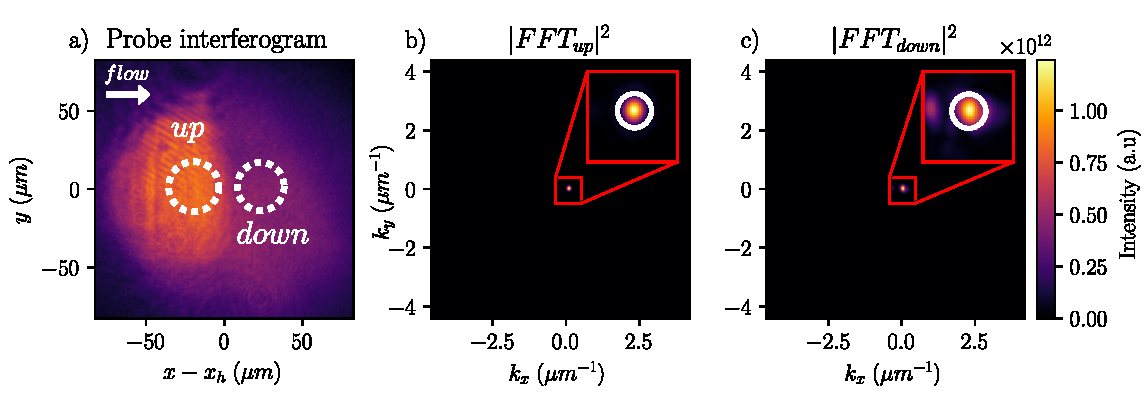
\includegraphics[width=1\textwidth]{chap_stimulated_hawking/fig/fft_bh_fluctu.pdf}
    \caption{\textbf{a) Probe interferogram.} The probe is located in the upstream region as in \autoref{fig:bh_density}. The white dashed circle represent the numerical mask applied to isolate each region.
    \textbf{b)} Shifted Fourier transform of the masked interferogram of the upstream region. The red inset is a zoom on a $\SI{0.2}{\per \micro \meter}$ region around the probe spot where the solid white circle correspond to the numerical pinhole applied to isolate the probe signal.
    \textbf{c)} Shifted Fourier transform of the masked interferogram of the downstream region. The red inset is a zoom on a $\SI{0.2}{\per \micro \meter}$ region around the probe spot where the solid white circle corresponds to the numerical pinhole applied to isolate the probe signal.}
    \label{fig:fft_bh_fluctu}
\end{figure}

\bigskip

\textbf{Spectrum reconstruction.} For each interferogram, a Gaussian numerical mask of width \SI{40}{\micro \meter} is applied either in the upstream or downstream region to spatially isolate the area of interest (see ~\autoref{fig:bh_density}). A two-dimensional Fourier transform is then performed on the masked interferograms, yielding the fluctuation spectrum at the probe frequency within the selected region.
Initially, our objective was to extract the Bogoliubov dispersion relation in each region, which, as discussed in the previous chapter, can be inferred from the transmission spectrum of the probe across the sample. To this end, an additional numerical pinhole (centered on the probe wavevector and with a radius matched to the probe spot) is applied in the Fourier domain of the interferogram, as illustrated in \autoref{fig:fft_bh_fluctu}.
The integral over the masked Fourier planes provides the transmission of the probe in the corresponding region.


In summary, for each probe configuration defined by the \((k_{in}, \omega_{in})\) couple, this procedure yields the transmitted probe intensity \(I_{u,d}(k_{in}, \omega_{in})\) in both the upstream and the downstream regions.
At this stage, the reason for positioning the probe beam so that it slightly overlaps with the downstream region becomes clear: it allows for the direct excitation of Bogoliubov modes with minimal influence from the interface. This is essential for benchmarking the dispersion relation of modes transmitted from upstream, and for confirming that they coincide with those excited locally in the downstream region.
By repeating this procedure while varying the probe wavevector and frequency we obtain the Bogoliubov dispersion in each region, as shown in \autoref{fig:fit_bogo}.  As anticipated, only the normal branch is accessible via direct excitation. This is not a limitation since this method was specifically chosen for its ability to isolate positive frequency signals. 
In addition, knowledge of the normal branch alone is sufficient to reconstruct the full Bogoliubov spectrum, as its structure is intrinsically symmetric with respect to the pump. Moreover, the existence of the ghost branch, particularly its positive-frequency domain, which is essential for the Hawking effect in the supercritical regime, was established in the previous chapter. Consequently, we will not attempt to measure it in this experiment.
\begin{figure}
    \centering
    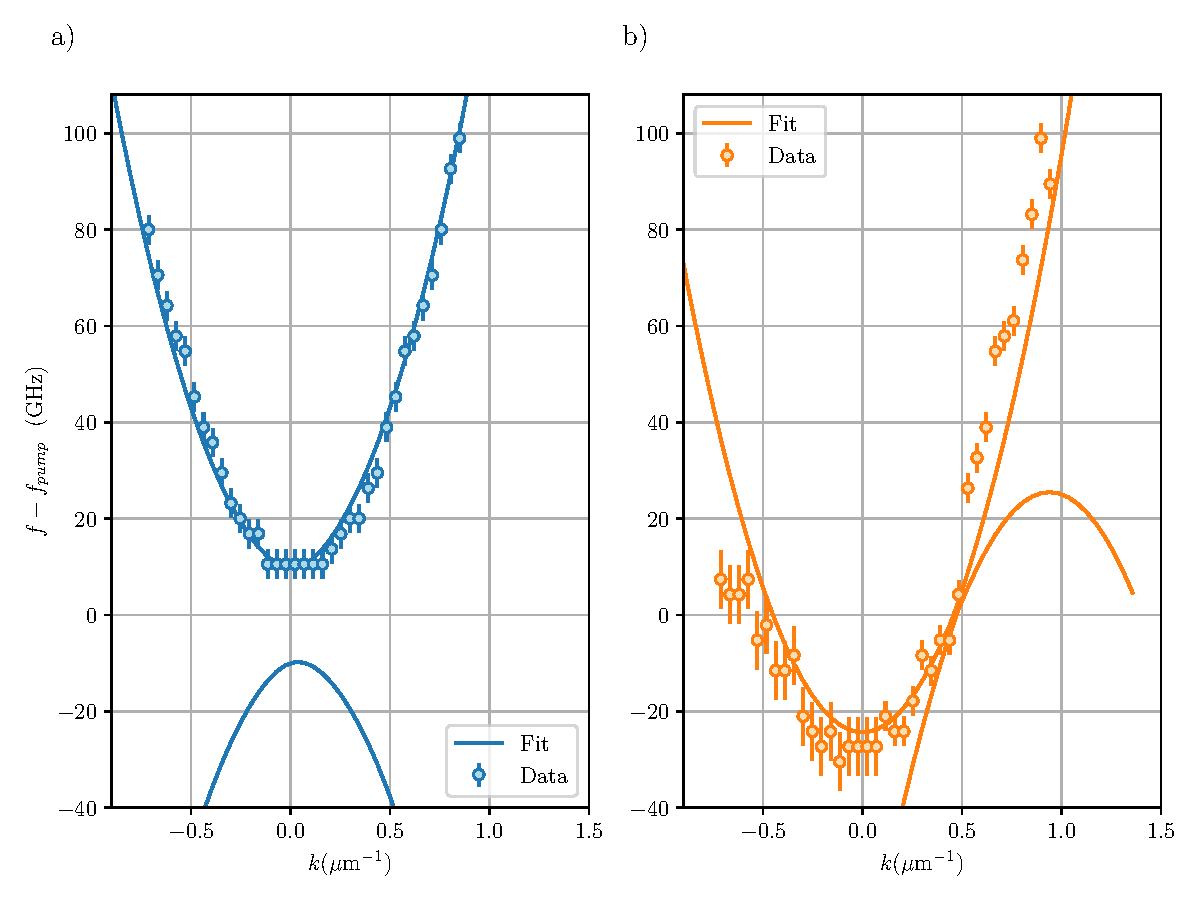
\includegraphics[width=1\textwidth]{chap_stimulated_hawking/fig/fit_bogo.pdf}
    \caption{\textbf{a)-b)} \textbf{Upstream-Downstream Bogoliubov spectrum}. The scattered points correspond to the maxima of the transmission spectrum of the probe in the upstream-downstream region. The blue-orange solid 
    line is the analytical Bogoliubov dispersion plotted with the experimental parameters and the nonlinear interactions $gn_0$ obtained from
    the fit of the data with the normal Bogoliubov branch. The upstream region fit gives $gn_0 =9.6 \pm \SI{0.1}{\giga \hertz}$ while in the downstream we obtain $gn_0=1.2\pm \SI{0.01}{\giga \hertz}$.
    The vertical error bars mainly originate from the frequency resolution of the measurement.}
    \label{fig:fit_bogo}
\end{figure}
\bigskip 

The upstream spectrum shown in \autoref{fig:fit_bogo}~\textbf{a)} exhibits a gap and a slight Doppler shift consistent with the pump wavevector in the upstream region $k_p=\SI{0.023}{\per \micro \meter}$. The data points are fitted with the Bogoliubov dispersion relation given in \autoref{eq:bogo_lab_frame} where $gn_0$ is the only fitting parameter (the dark reservoir
is handled in the same way as in the previous chapter ie set to $g_rn_r=1.84gn$). 
We obtain $gn_0=9.6\pm\SI{0.1}{\giga \hertz}$ and find a good agreement of the model with the experimental points.

The downstream spectrum shown in \autoref{fig:fit_bogo}~\textbf{b)} features negative frequency modes, which is typical of a supercritical flow.
In the absence of pumping, the system must satisfy the condition given in \autoref{eq:bernoulli}, which can be recast in the form $\delta(k_{fluid})=gn_0+g_rn_r$. It is the counterpart of the turning point condition in the pumped region, implying that the Bogoliubov spectrum is expected to be linear at low $k$ far from the interface:
\begin{equation}
    \omega_B(k) = v_d(k-k_d) \pm \sqrt{\dfrac{\hbar (k-k_d)^2}{2\mlp} \left({\dfrac{\hbar (k-k_d)^2}{2\mlp}} + g n_0 \right)},
\end{equation}
where $v_d = \hbar k_d/\mlp$ is the asymptotic velocity of the fluid measured by off-axis interferometry. The fit gives $gn_0=\SI{1.2 \pm 0.01}{\giga \hertz}$. As visible in \autoref{fig:fit_bogo}~\textbf{b)}, the agreement is not as good as in the upstream region. 
This is because in the unpumped region, the fluid is no longer homogeneous close to the interface, as shown in \autoref{fig:bh_balistic} \textbf{b)}.
Homogeneity is recovered far from the interface, where the density is low, implying that there is no fluid left to probe.
Consequently, the measured signal comes mainly from the transient region, where looking for the Bogoliubov modes as plane waves is already an approximation.
To obtain a better agreement between the theoretical curve and the experimental data, a complete diagonalization of the Bogoliubov matrix around the steady state would be necessary in this region to obtain the exact expected Bogoliubov spectrum. However, this is not the goal of this work, and the supercritical feature we are interested in
remains robust against this approximation.

The shape of the spectrum in each region indicates the presence of an acoustic horizon.
We can now turn to the measurement of the scattering matrix.

\subsection{Observation of stimulated Hawking radiation}
\label{sec:scattering_matrix}

\subsubsection{Detection of the scattered modes}

We analyze the emergence of transmitted or reflected modes resulting from the scattering of a perturbation impinging on the horizon from the upstream region, namely when the probe excites a \( u_{in}(k) \) mode. 


For each $k_{in}$, we compute the Fourier transform of the probe interferogram in both the upstream and downstream regions, following the same separation procedure used for the reconstruction of the Bogoliubov spectrum. 
In contrast to the earlier analysis, we now apply a numerical anti-pinhole in the Fourier plane to suppress the intense contribution of the \( u_{in} \) mode at the probe position. A peak detection algorithm is then used to identify the positions of the scattered modes in the Fourier plane and to extract their wavevector.
Each identified wavevector is compared with the Bogoliubov spectrum to confirm its physical relevance and to rule out spurious scattering events. This process is systematically repeated as the probe sequentially excites each $u_{in}$ mode. The resulting scattering data are summarized in \autoref{fig:fit_bogo_RT} \textbf{a)}. As observed, the $(k,\,\omega)$ positions of the modes detected both in the upstream and downstream regions agree well with the Bogoliubov dispersions.

\begin{figure}
    \centering
    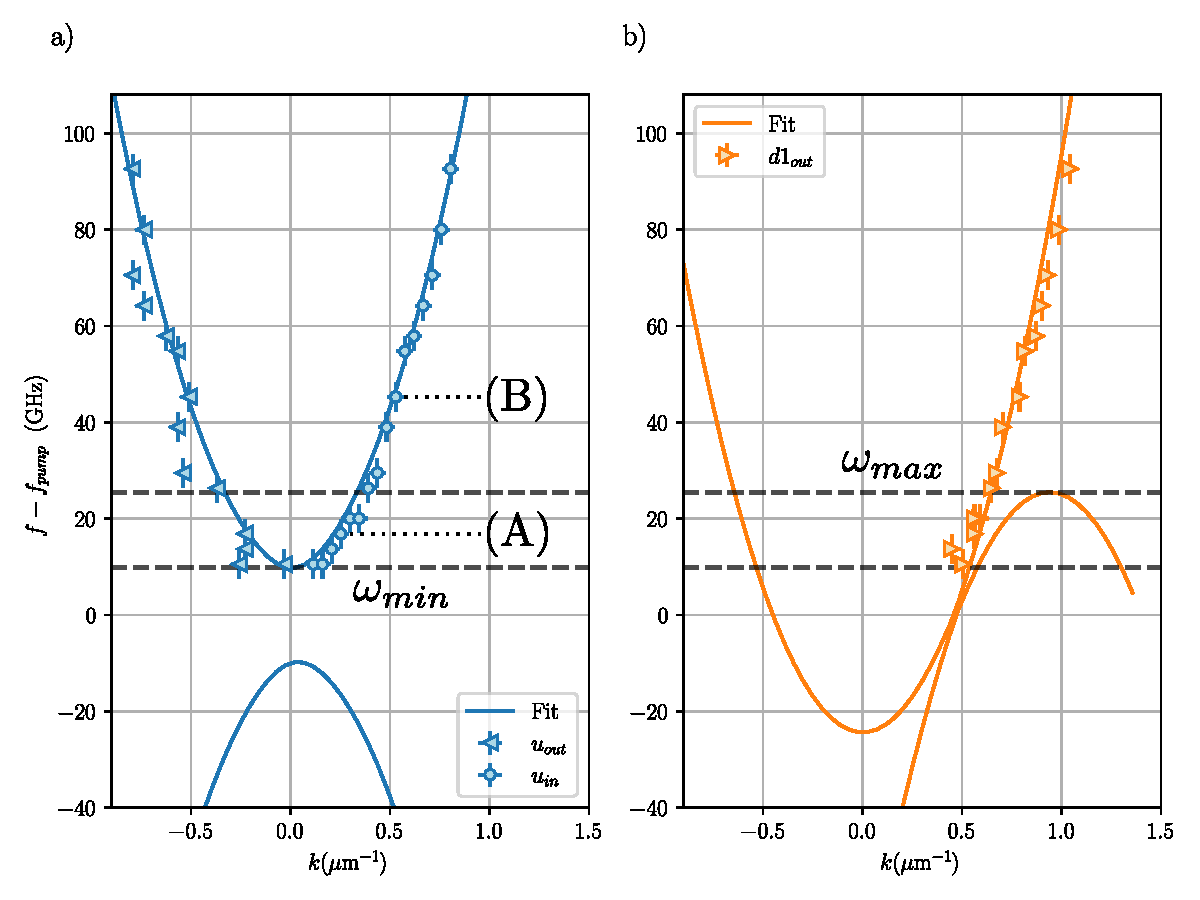
\includegraphics[width=1\textwidth]{chap_stimulated_hawking/fig/fit_bogo_RT.pdf}
    \caption{
    \textbf{Reflection and transmission at the horizon.}
    \textbf{a) Measurement of the reflected modes $u_{out}$} The $u_{in}$ modes excited by the probe are represented by the blue dots. The error bars are the same as in \autoref{fig:fit_bogo}. For each $u_{in}$ mode,
    the wavevectors of the maxima detected in the upstream region are represented by the blue left-oriented triangles. The error bars are the same than for the $u_{in}$ modes with an additional contribution due to the resolution in momentum space ($\Delta=\SI{0.027}{\per \micro \meter}$) in the peak detection algorithm.
    The blue solid line is the fit of the upstream Bogoliubov dispersion obtained in \autoref{fig:fit_bogo}~\textbf{a)}.
    The black dashed lines define the frequency range at which negative-positive energy mixing is possible.
    The specific configurations $\mathrm{(A)}$ and $\mathrm{(B)}$ are taken as examples for later comparison. The mode $\mathrm{(A)}$ lies in the negative-positive energy mixing frequency interval, while the mode $\mathrm{(B)}$ lies outside.
    \textbf{b) Measurement of the transmitted modes.} The wavevectors of the maxima detected in the downstream region are represented by the orange right-oriented triangles. The error bars are the same as in \textbf{a)}. 
    The orange solid line is the fit of the downstream Bogoliubov dispersion obtained in \autoref{fig:fit_bogo} \textbf{b)}. }
    \label{fig:fit_bogo_RT}
\end{figure}

This measurement demonstrates that the interface scatters the incoming modes as expected from the Bogoliubov theory. However, the $d2_{out}$ modes --that are expected on the ghost branch--are not detected in the downstream region. This is due to its negative norm: its amplitude mostly lies on the conjugate branch.
Indeed, in the Bogoliubov basis the excited $d2_{out}$ mode is written as :
\begin{equation}
    \begin{pmatrix}
        u_{k_{d2}^{out}} \\
        v_{k_{d2}^{out}}
    \end{pmatrix}e^{-i\omega_{pr}t}=
    \begin{pmatrix}
    U_{k_{d2}^{out}} \\
    V_{k_{d2}^{out}}
    \end{pmatrix}e^{ik_{d2}^{out}x}e^{-i\omega_{pr}t}, 
\end{equation}
where $\omega_{pr}$ is the probe frequency. According to ~\ref{eq:fluctuation_order_parameter}, the corresponding fluctuation of the order parameter ie the physical quantity experimentally accessible, is :
\begin{equation}
    \delta\psi_{{d2_{out}}}(x,t)= U_{k_{d2}^{out}}e^{ik_{d2}^{out}x}e^{-i\omega_{pr}t}+V_{k_{d2}^{out}}^*e^{-ik_{d2}^{out}x}e^{i\omega_{pr}t}.
    \label{eq:order_param_d2_out}
\end{equation}
Due to its negative norm the Bogoliubov amplitudes are $\int |U_{k_{d2}^{out}}|^2-|V_{k_{d2}^{out}}|^2=-1$, meaning that  $|V_{k_{d2}^{out}}|^2$ is significantly greater than $|U_{k_{d2}^{out}}|^2$. 
Consequently, its larger amplitude is at opposite frequency and wavevector, namely, in the $d2_{out}^*$ mode (on the normal branch at negative frequency). This explains why the interferometric technique, which 
can detect only modes at the probe frequency fails to detect the weak amplitude of the $d2_{out}$ mode.

To measure amplitudes in $d2_{out}^*$, we use an imaging spectrometer Princeton Instruments SpectraPro SP-2750 mounted with a 1200 lines/mm grating together with a high sensitive CCD camera Teledyne PIXIS 1024. By imaging the Fourier plane of the entire field on the entrance slit of the spectrometer it is possible to directly obtain the spectrum of the fluid including both the pump and the probe contributions.
As the pump is generally two orders of magnitude brighter than the probe, it quickly saturates the camera sensor, preventing the detection of weak probe signals.
To overcome this issue, the pump is filtered out by a rasor blade placed in real space, before the spectrometer. The blade is positioned so as to block the bright upstream region while letting the weak downstream region pass through.
This allows setting a long exposure time without being blinded by the pump. A typical spectrum taken with a 4 seconds exposure time is shown in \autoref{fig:spectrum_spectro}~\textbf{a)}. By superimposing the image with the downstream Bogoliubov dispersion obtained earlier, the different modes are identified.
Their positions are represented by colored dashed circles in \autoref{fig:spectrum_spectro}~\textbf{a)}.

\bigskip

Remarkably, an intensity peak is observed at the $d2_{out}^*$ mode, as shown in the vertical cut in \autoref{fig:spectrum_spectro}\textbf{b)}. To confirm that this mode indeed originates from Hawking radiation, we verified that the peak disappears when the excited $u_{in}$ mode lies outside the negative–positive energy mixing frequency interval.


Finally, an additional peak is observed at $\omega = 2\omega_{probe}$ indicated by the green dashed circle in \autoref{fig:spectrum_spectro} \textbf{a)}. We interpret it as the result of a four-wave mixing process where two $d1_{out}$ polaritons scatter into a pump mode polariton and a higher energy mode:
\begin{equation}
    \begin{aligned}
    (\omega_{pr}, \omega_{pr}) &\to (0, 2\omega_{pr}) \\
    (k_{d1}^{out}, k_{d1}^{out}) &\to (k_{d1}^{out}-\Delta k,k_{d1}^{out}+\Delta k),
    \end{aligned}
    \label{eq:higher_order_four_wave_mixing}
\end{equation}
where $\Delta k=k_{d1}^{out}-k_d$ is the wavevector mismatch between the pump in the downstream region and the $d1_{out}$ mode. This process arises as a consequence of bosonic stimulation resulting from the high occupancy of the pump state, while the linearity of the Bogoliubov spectrum ensures optimal phase matching.

\bigskip

The simultaneous detection of modes $u_{out}$, $d1_{out}$ and $d2_{out}^*$ when the probe is exciting a $u_{in}$ mode in the negative-positive energy mixing region is a convincing signature of stimulated Hawking radiation. Let us now turn to a more quantitative analysis and see whether reflection and transmission coefficients can be extracted from the data.

\begin{figure}
    \centering
    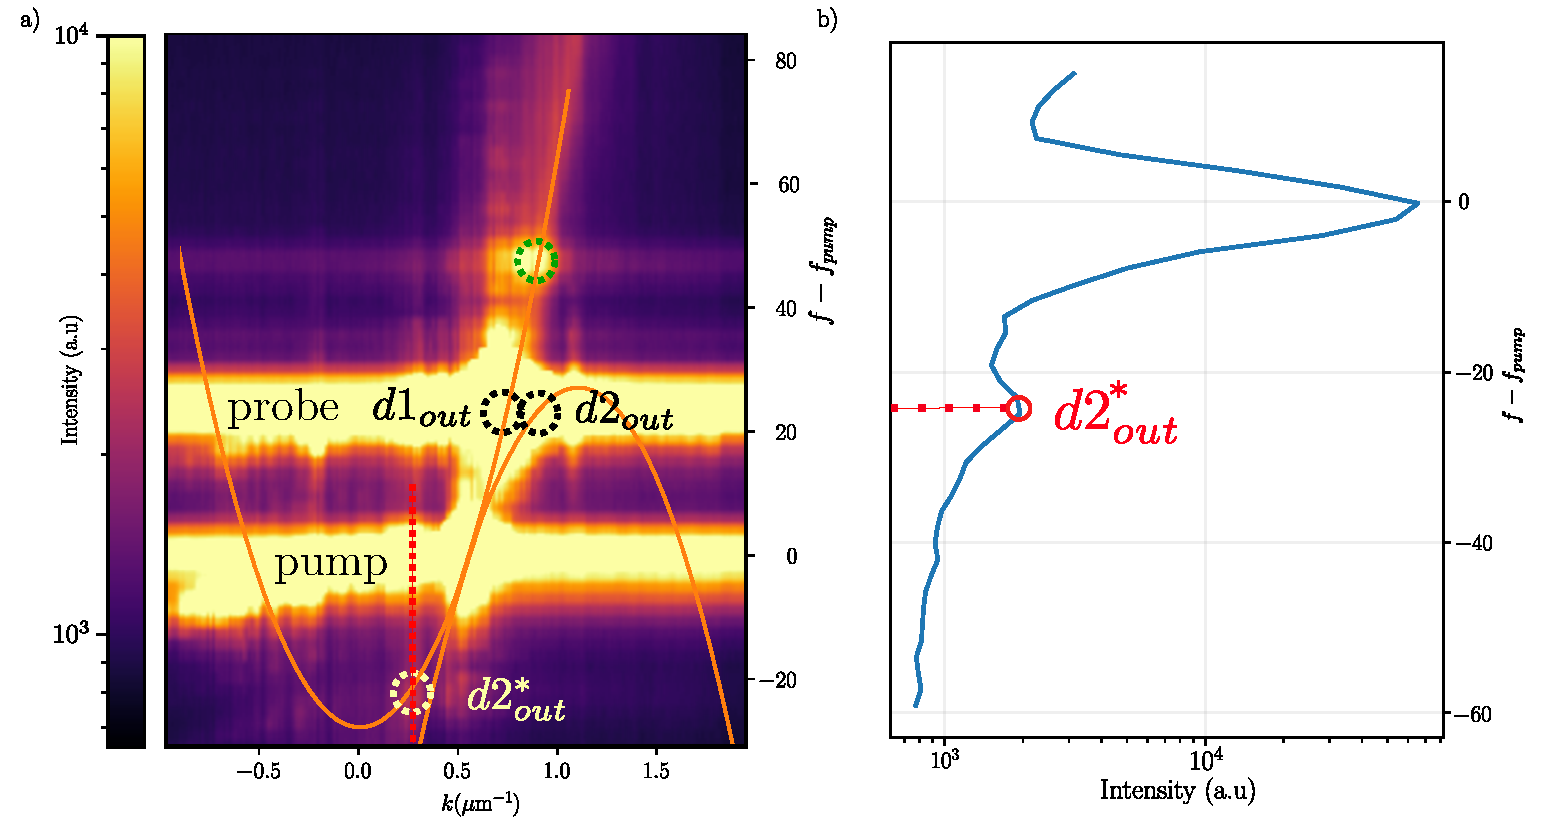
\includegraphics[width=1\textwidth]{chap_stimulated_hawking/fig/disp_supersonic_spectro.pdf}
    \caption{\textbf{a) Spectrum of the downstream region of the fluid.} The spectrum is obtained by integrating over the whole downstream region of the fluid during 4 seconds
    with an imaging spectrometer. The bright horizontal lines labelled pump and probe are due the saturation of the camera sensor by the probe and pump. The orange solid line represents the fit of the Bogoliubov dispersion relation obtained in \autoref{fig:fit_bogo} \textbf{b)}. The dashed purple circles are 
    the $d1_{out}$ mode and the expected location of the $d2_{out}$.
    The orange dashed circle is the $d2_{out}^*$ mode, conjugate of $d2_{out}$. The green dashed circle represents a higher order four-wave mixing at twice the probe frequency. The red dashed line indicates the energy cut made in the right subplot.
    \textbf{b) Vertical cut of the $d2_{out}^*$ mode.} The intense peak on the right corresponds to the remaining pump contribution. The red dashed line is the $d2_{out}^*$ mode energy.}
    \label{fig:spectrum_spectro}
\end{figure}
\bigskip

\subsection{Toward the measurement of the scattering matrix}
\label{sec:scattering_matrix_measurement}
\subsubsection{Input and output modes discrimination}
In order to compute reflection and transmission coefficients, the input and output modes must be defined clearly.
To do so, let us consider the perturbation field $\delta\psi$ when a $in$ mode is excited. In a first approach, we restrict our description to what is experimentally accessible with our interferometric method.
Namely, the field at the probe frequency only. In a very general way, the wavefunction can be decomposed as follows:
\begin{equation}
    \begin{aligned}
    \delta\psi(x,t) &= \delta \psi_\mathrm{in}(x,t)+\delta \psi_\mathrm{res}(x,t) \\
    &= \delta \psi_{in}(x,t) + \delta \psi_\mathrm{scat}(x,t) + \delta \psi_\mathrm{err}(x,t).
    \end{aligned}
\label{eq:scat_decomp}
\end{equation}
where $\delta \psi_\mathrm{in}$ is the ideal incoming mode ie a perfect gaussian of the form :
\begin{equation}
\delta \psi_\mathrm{in}= \mathrm{A} e^{\frac{-(x-x_{in})^2}{w}}e^{ik_{in}x}
\end{equation}
where $w$ is the width of the mode and A its amplitude. Note that this is the continuous wave counterpart of the probe beam defined in the numerical study \cite{carusotto_fluidlightproposal_2012}.
Conversely, $\delta \psi_\mathrm{res}$ is the residual field. The latter is made of all the other modes that are not in the $in$ mode. The term $\psi_\mathrm{scat}$ represents all the scattering events that may occur in the fluid. In particular, it contains the outgoing modes $u_{out}$, $d_1^{out}$ and $d_2^{out}$ that are the result of the scattering at the horizon. Furthermore, the residual field also accounts for deviations
of the injected probe beam in the cavity from the perfect Gaussian beam defined by $\delta \psi_{in}(x,t)$. This contribution $\delta \psi_\mathrm{err}(x,t)$ is purely optical and can be thought of as a bias when $\psi_\mathrm{in}$ is extracted from the true probe beam, as we shall see now.

\bigskip

\textbf{Input mode.} The most reliable method to define the $in$ mode while minimizing potential biases is to perform a Fourier transform of the perturbation field and apply a modal decomposition.
 Following the procedure outlined in the previous section, we first identify the amplitude peak of the injected mode, which constitutes the dominant contribution in Fourier space. 
 Cuts along both axes of the detected peak are presented in \autoref{fig:fit_input_mode}~\textbf{a)} and \textbf{b)}.
Noticeably, the peak is not perfectly symmetric and shows a slight elongation along the \( k_x \) direction. 
It remains unclear whether this asymmetry carries information about the scattering process itself or whether it merely results from the broadening induced by the fluid's motion. 
To address this ambiguity, we focus on the \( k_y \) direction, exploiting the translational invariance of the fluid along this axis, as discussed in \autoref{chap:AG_theory}. 

The cut along the \( y \)-axis is then fitted with a one-dimensional Gaussian function of the form
\[
f(k_y) = \mathrm{A} \exp\left( -\frac{(k_y - k_y^0)^2}{2\sigma^2} \right)
\]
The resulting fit is shown in \autoref{fig:fit_input_mode}~\textbf{a)}, demonstrating excellent agreement with the data. The amplitude \( \mathrm{A} \) and width \( \sigma \) obtained from the fit are then used to define a two-dimensional Gaussian function with the same amplitude and width, centered on the wavevector \( \mathbf{k}=(k_x^0,k_y^0)=(k_{in},0)\):
\begin{equation}
    \mathrm{A_{fit}}(k_x,k_y) = \mathrm{A} \mathrm{exp}(-\frac{(k_x-k_x^0)^2}{2\sigma^2}-\frac{(k_y-k_y^0)^2}{2\sigma^2}).
    \label{eq:gaussian_amp} 
\end{equation}

To end the definition of the input mode complex field, we need to provide it with a phase. To do so, we look at the phase of the $\delta \tilde{\psi}$ 
in the vicinity of the peak. Close to the maximum amplitude, the phase is well defined and is approximated by a planar surface by fitting the signal with a function of the form $\theta_{fit}(k_x, k_y)=x_0k_x+y_0k_y+c$ where $x_0$, $y_0$ and $c$ are the fitting parameters.
These encode the position of the $in$ mode in real space.
This fitting procedure is equivalent to neglecting any curvature in the mode wavefront or, in other words, to assume that the mode has a plane wave phase.
Of course, fluctuations around this ideal phase are expected and may contain information about the scattering process.
To take this into account, we perform a last step that consists of projecting the overall field $\delta \tilde{\psi}$ on the ideal input mode we just defined, ie, $\delta \tilde{\psi}_{\mathrm{fit}}(\kvec)= \mathrm{A_{fit}}(\kvec)\mathrm{exp}(i\theta_{\mathrm{fit}}(\kvec))$.
The resulting field is given by :
\begin{equation}
    \delta \tilde{\psi}_{in} = \bra{\delta \tilde{\psi}_{\mathrm{fit}}}\ket{\delta \tilde{\psi}} \delta \tilde{\psi}_{\mathrm{fit}}. 
    \label{eq:input_mode_scalar_product}
\end{equation}

\bigskip 

\textbf{Residual field.} From the above expression, we are able to define the residual field as the difference between the injected mode and the overall field $\delta \tilde{\psi}_{res} = \delta \tilde{\psi}-\delta \tilde{\psi}_{in}$. 
Note that the way $\delta \tilde{\psi}_{in}$ is built through a scalar product ensures that the residual field is orthogonal to the $in$ mode provided $\delta \tilde{\psi}_{fit}$ is normalized:
\begin{equation}
    \begin{aligned}
    \bra{\delta \tilde{\psi}_{in}}\ket{\delta \tilde{\psi}_{res}} &=\bra{\delta \tilde{\psi}_{\mathrm{fit}}}\ket{\delta \tilde{\psi}} \left(\bra{\delta \tilde{\psi}_{\mathrm{fit}}}\ket{\delta \tilde{\psi}} - \bra{\delta \tilde{\psi}_{\mathrm{fit}}}\ket{\delta \tilde{\psi}_{in}}\right)\\
    &= \bra{\delta \tilde{\psi}_{\mathrm{fit}}}\ket{\delta \tilde{\psi}} \left(\bra{\delta \tilde{\psi}_{\mathrm{fit}}}\ket{\delta \tilde{\psi}}-\bra{\delta \tilde{\psi}_{\mathrm{fit}}}\ket{\delta \tilde{\psi}_{\mathrm{fit}}}\bra{\delta \tilde{\psi}_{\mathrm{fit}}}\ket{\delta \tilde{\psi}}\right)\\
    &=0.
    \end{aligned}
\end{equation}
In this manner, the basis chosen for our description is as close as possible to the Bogoliubov plane wave basis explicitly specified in \autoref{chap:AG_theory}. This is a strong assumption that will be discussed in the following. 


\subsubsection{Real space analysis}
In the previous section, the different modes involved in the scattering process were well separated in momentum space. In this modal picture, the natural procedure to obtain reflection and transmission coefficients seems
to be the comparison between the amplitudes of the different modes in momentum space. Indeed, in an ideal situation where the only modes involved in the scattering process are the incoming and outgoing modes --or said differently where $\delta\psi_{err}=0$-- each mode results in a well-defined peak in the Fourier plane whose maximum and position are directly related to the amplitude and wavevector of the modes, respectively. 


In the present case, the situation is quite different, as the residual field $\delta \psi_{res}$ is not negligible. To illustrate this point, we performed the inverse Fourier transform of the fields and analyzed the resulting images in real space.
The results are shown in \autoref{fig:fit_input_mode}~\textbf{c)} and \textbf{d)}. As expected, the input mode is very close to a perfect Gaussian beam since it was constructed precisely to be such.
The residual field, on the other hand, is much more complex and contains spurious contributions. For example, the signal is not zero far from the interface in the upstream region as visible on the intensity cut in \autoref{fig:fit_input_mode}~\textbf{e)} near $x\approx -\SI{60}{\micro \meter}$. This would not be the case if $\psi_{res}$ consisted solely of reflected or transmitted signals at the interface. More specifically, the profile in \textbf{e)} would instead be composed of two decaying exponentials, both originating from the horizon.
Indeed, the discussion made in \autoref{sec:ballistic_configuration} also holds for the Bogoliubov modes, meaning that the scattered modes --that are not supported by the probe laser--
are exponentially damped with a characteristic length fixed by their group velocity and the polariton lifetime as in \autoref{eq:bernoulli}.


This demonstrates that the way we defined the $in$ mode indeed introduces a bias. Therefore, a direct analysis in Fourier space would include many unwanted contributions, making quantitative analysis difficult. 
A more reliable method is to analyze the data locally in real space in the vicinity of the horizon. This is what is done in analytical works \cite{Recati_acousticHR_2009,carusotto_fluidlightproposal_2012} where the scattering matrix coefficients are computed from the continuity equations of the wavefunctions and their derivatives at the horizon \cite{rot_supperradiance_delhom}. This approach is particularly well suited to stationary flows, where the time variable is eliminated. It is the standard method used to solve textbook quantum mechanics problems \cite{CCT_tome1}, such as the scattering of a plane wave incident from $-\infty$ by a potential barrier. In this case, the reflection and transmission coefficients can be obtained by taking the ratio of the complex amplitudes of the reflected and transmitted waves to the amplitude of the incoming one at the interface. Usually, this cannot be done experimentally since the field at a given position is a superposition of all the modes present. Consequently, unless having a perfect knowledge of the incoming mode both in phase and amplitude, an intensity measurement does not allow to discriminate between the different contributions because of the interference between them.


In our case, the interferometric method together with the procedure of separating the modes in momentum space and then performing the inverse Fourier transform allows analyzing the complex fields independently. However, a local analysis does not remove the spurious contributions of the residual field even in the vicinity of the interface.


\begin{figure}
    \centering
    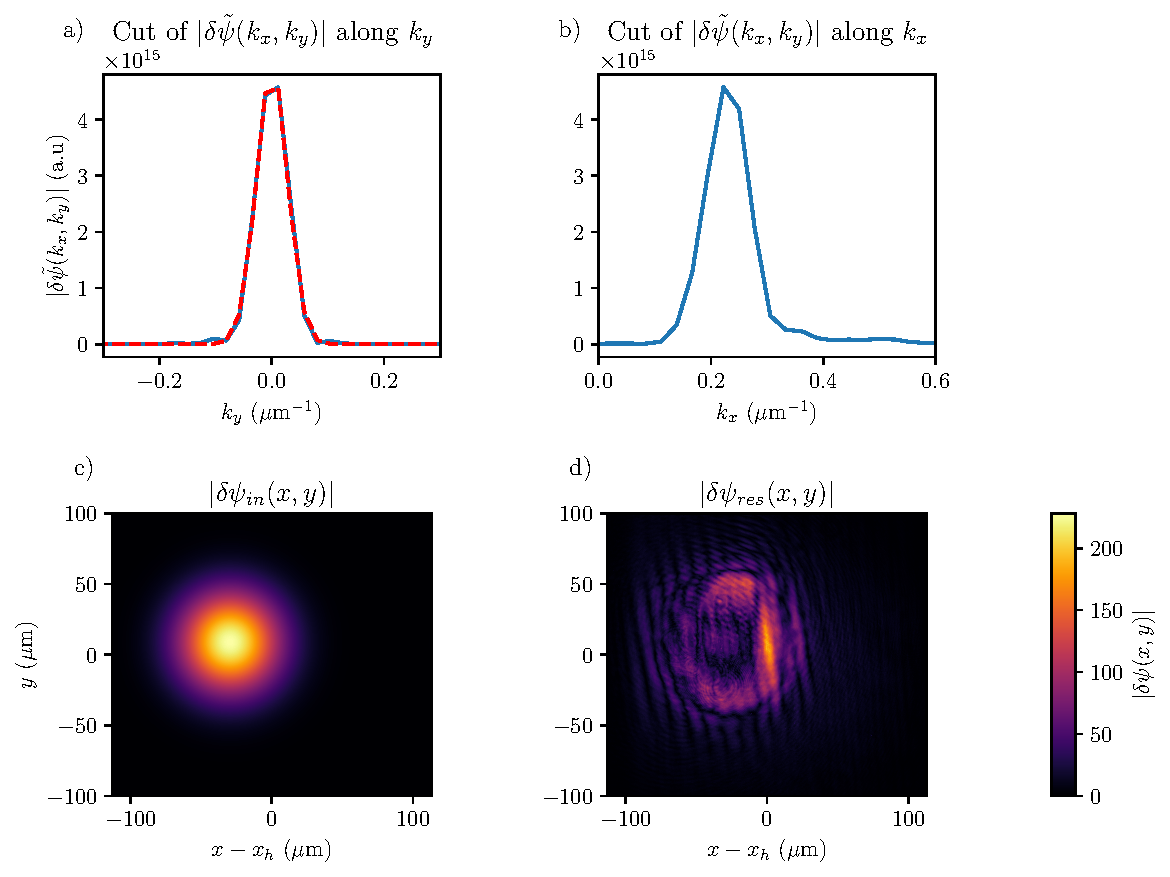
\includegraphics[width=1\textwidth]{chap_stimulated_hawking/fig/fit_input_mode.pdf}
    \caption{\textbf{a) Cut of the injected mode in the $k_y$ direction.} The blue curve is the data and the red dashed curve is the gaussian fit. The model has a R-squared value of 0.98. The amplitude $A$ and width $\sigma$ are extracted from the fit. 
    \textbf{b) Cut of the injected mode in the $k_x$ direction.}
    \textbf{c) Intensity of the constructed input mode in real space.} Obtained by applying the inverse Fourier transform to $\delta \psi_{in}(k_x,k_y)$.
    \textbf{d) Intensity of the constructed residual field in real space.} Obtained by applying the inverse Fourier transform to $\delta \psi_{res}(k_x,k_y)$.
    \textbf{e) Cut of the intensity of the residual field.} An average along the $y$ axis is performed in the region of interest (ROI) defined by the white dashed rectangle of \textbf{d)}.}
    \label{fig:fit_input_mode}
\end{figure}


\subsubsection{Signature of amplification}
Although the previous section highlighted the potential inaccuracies introduced by the modal decomposition, the method remains a robust and systematic approach to define the various modes, independently from specific experimental realizations. That is, the relative energy contribution of the $in$ mode to the total energy remains invariant across different probe configurations, indicating that the bias in the field decomposition is effectively independent of which specific $in$ mode is excited.
To illustrate this point, we calculate the energy \( \int \mathrm{d}\mathbf{r} \, |\delta\psi_i(\mathbf{r})|^2 \) associated with each mode, as well as the total energy, as functions of the probe wavevector. The results are presented in \autoref{fig:energy_budget}. 
The subpanel \textbf{b)} shows that the ratio \( E_{in}/E_{tot} \) remains approximately constant at 0.79 with a standard deviation of 0.02.  


Moreover, it should be noted that the sum of the energies in the \( in \) and \( out \) modes precisely equals the total energy, as evident in \textbf{a)}. Whereas this feature appeared obvious in momentum space since the modes were orthogonal by construction, it is less trivial in real space.
In fact, the residual and scattered fields spatially overlap, giving rise to an interference term of the form $\delta \psi_{res}^*(\rbf) \delta \psi_{scat}(\rbf)$. In fact, this term sums up to zero when integrated over the whole space.
This is a direct consequence of the Fourier transform isometry property which conserves the $L^2$ scalar product.

\bigskip

To summarize, our method defines the input and output modes in a manner that is independent of the specific experimental realization. Consequently, variations in the relative contributions of individual modes across different configurations carry physical information about the interaction between the input mode and the interface. 
 \begin{figure}
    \centering
    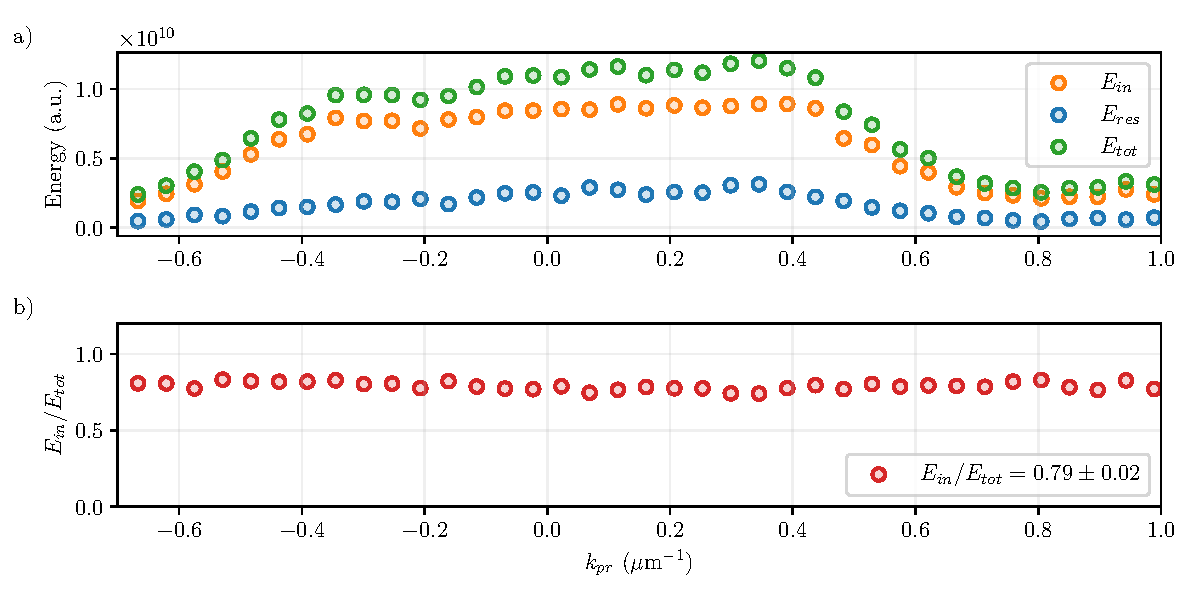
\includegraphics[width=1\textwidth]{chap_stimulated_hawking/fig/energy_budget.pdf}
    \caption{\textbf{a) Energy budget.} The energy in the $in$ mode (orange) the $res$ mode (blue) and the total energy (green) are plotted as a function of the probe wavevector. 
    \textbf{b) Ratio of the energy in the $in$ mode with respect to the total energy.} The average value is 0.79 with a standard deviation of 0.02.}
    \label{fig:energy_budget}
 \end{figure}

\bigskip

To observe a signature of amplification, we compare two specific configurations: when the input modes lie in the negative-positive energy mixing interval (configuration A) and when it lies outside of it (configuration B). The specific 
realizations taken for comparison are labeled in \autoref{fig:fit_bogo_RT}~\textbf{a)}. For both configurations, a cut of the intensity in the $x$ direction is done for each mode. To smooth the data and enhance the signals, an average along the $y$-axis in the region of interest (ROI) defined by the white dashed rectangle of \autoref{fig:fit_input_mode}~\textbf{d)} is performed. 
The results are shown in \autoref{fig:intensity_comparison}. The first observation is that, in both configurations, the residual mode yields an intensity spike at $x=x_h$ reflecting that the residual field is in fact mostly located at the interface. 

However, the shape of the residual field is an additional proof that our mode decomposition was not perfect. Indeed, as explained in the previous section, if the residual field consisted solely of scattered modes, the resulting intensity profile would exhibit two decaying exponentials with distinct characteristic lengths.
One oriented toward the upstream region with characteristic length $l_u=v_u/2\gamlp$ where $v_u$ is the $u_{out}$ mode group velocity, and another oriented toward the downstream region corresponding primarily to $d1_{out}$ with characteristic length $l_{d1}=v_{d1}/2\gamlp$. Furthermore, as remarkable in \autoref{fig:fit_bogo_RT}, $|v_{d1}|$ is always greater than $|v_u|$ meaning that the upstream exponential should decrease faster the downstream one. This is not what we observed and the displayed profile seems actually to present the opposite behavior.
This being said, it does not prevent us from comparing the two configurations.


In configuration (B) the $res$ mode intensity is significantly lower than the $in$ mode and never exceeds it, whereas in configuration (A) where amplification is expected, the $res$ mode intensity becomes larger than that of the $in$ mode at the interface.
For comparison purposes, we compute the intensity ratios at the interface for both cases. In configuration (B), be obtain $I_{res}/I_{in} = 0.15$ while in configuration (A) we find $I_{res}/I_{in} = 1.89$. This indicates that whenever the input mode lies in the negative-positive energy mixing region, the relative contribution of the residual mode
is significantly higher than when it lies outside this frequency interval, while the $in$ mode remained the same. 

\begin{figure}
    \centering
    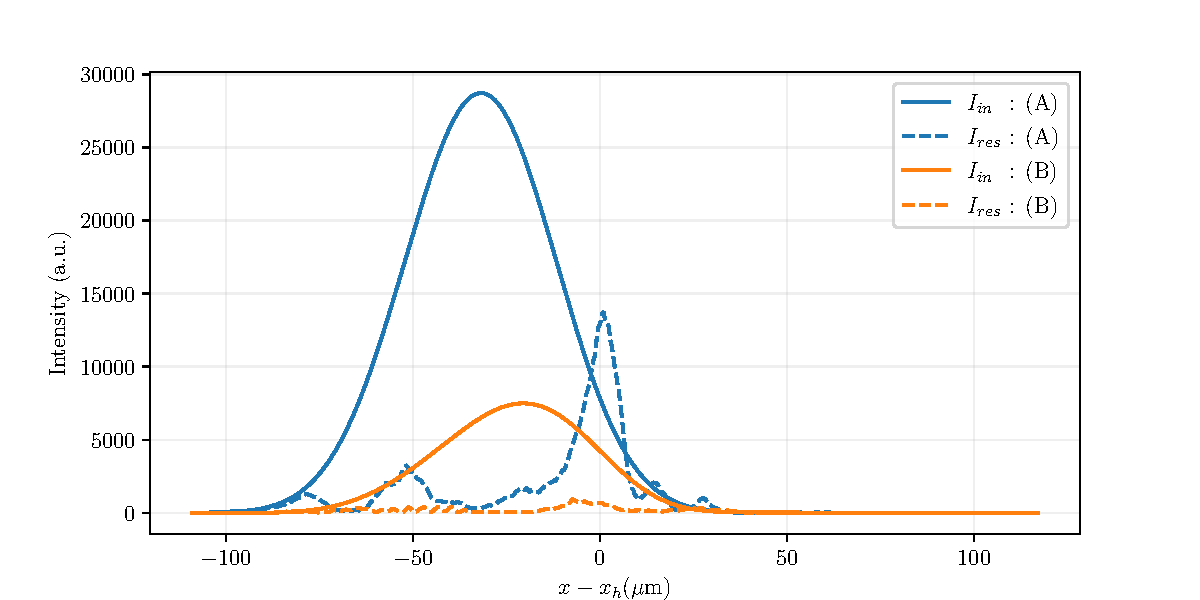
\includegraphics[width=1\textwidth]{chap_stimulated_hawking/fig/intensity_comparison.pdf}
    \caption{\textbf{a) Intensity comparison}. Cuts along the $x$ direction of the intensities of the $in$ mode and the $res$ mode for the two configurations $\mathrm{(A)}$ and $\mathrm{(B)}$.
    The blue color corresponds to the $\mathrm{(A)}$ configuration in which the input mode lies in the negative-positive energy mixing region while the orange color corresponds to the $\mathrm{(B)}$ configuration in which the input mode lies outside this region.
    The solid lines are the $in$ mode intensities while the dashed lines are the $res$ mode intensities.}
    \label{fig:intensity_comparison}
\end{figure}

To highlight that this enhancement arises from the Hawking effect, we computed this ratio for all the $u_{in}$ mode. In each case, we take the left and right limit of the ratio $I_{res}(x)/I_{in}(x)$  labeled $L_u$ and $L_d$ respectively :
 
\begin{equation}
    \begin{aligned}
        L_u \coloneqq &\lim_{x\to x_H^-}I_{res}(x)/I_{in}(x) \\
        L_d \coloneqq &\lim_{x\to x_H^+}I_{res}(x)/I_{in}(x)
    \end{aligned}
\end{equation}
In practice, our measurements are not continuous and we compute the ratio at discrete positions $x_i$ in the vicinity of the horizon position $x_h$. More precisely,
the left (resp. right) limit is then computed by taking the ratio at the closest position $x_i$ to the left (resp. right) of $x_h$.      
These coefficients embed contributions from and the $u_{out}$ and $d1_{out}$ reflection and transmission and thus give information on the $|S_{uu}|^2$ and $|S_{d1u}|^2$ coefficients.
The results are presented in \autoref{fig:I_ratio_bary}~\textbf{a)} and clearly demonstrate the amplification of the residual field within the negative–positive energy mixing interval.


The error bars displayed come mainly from two sources: the uncertainty on the horizon position and the standard deviation of the energy ratio $E_{in}/E_{tot}$ calculated above.
Regarding the horizon position, it was initially defined as the position at which the speed of sound $c_s=\sqrt{gn_0/\mlp}$ equals the fluid velocity $\vbf_0$ while the previous chapter made clear
that this velocity is not the relevant one to define the interface. Indeed the critical velocity $v_c$ at which negative energy modes arise is greater than $c_s$. It means that computing the intensity ratios at $x=x_h$ may introduce an error. Quantifying this uncertainty precisely is difficult since the discrepancy between $v_c$ and $c_s$ velocities does not follow a simple law and depends on the fluids parameters. However, it is reasonable to assume that the horizon position lies within the upstream to downstream transition region of the fluid velocity (see Fig \ref{fig:bh_balistic}), which is of the order of $\sigma_{x_h}=\SI{5}{\micro \meter}$.
To propagate this uncertainty in the coefficients, we computed the intensity ratio at the left and right limits of position $x_i$ where $x_i \in [x_h-\SI{5}{\micro \meter}, x_h+\SI{5}{\micro \meter}]$. Then,
the mean values (resp. standard deviation) of the reflection and transmission coefficients are taken as the average (resp. standard deviation) of the left and right limits for all values of $x_i$. 

The second main source of uncertainty comes from the energy ratio $E_{in}/E_{tot}$, which is computed from the energy budget shown in \autoref{fig:energy_budget}~\textbf{b)}.
In other words, it ultimately originates from the procedure used to define the $in$ and the $res$ modes that, as already mentioned, is not perfect.
Once again, it is complicated to report this uncertainty on our local measurements since it was initially obtained by integrating fields over the entire space for all configurations.
We roughly estimate it by assuming that the relative error on the intensities is the same as the relative error on $E_{in}/E_{tot}$ divided by the area corresponding to the full field of view over accessible with our imaging system that is $226\times\SI{271}{ \micro \meter \squared}$. In other words, this hypothesis correspond to consider that the error on 
$\int |\delta \psi(r)|^2\mathrm{dr}$ is uniformly distributed over the integration area.

These two contributions are then added quadratically to obtain the final error bars shown in \autoref{fig:I_ratio_bary}~\textbf{a)}.

\begin{figure}
    \centering
    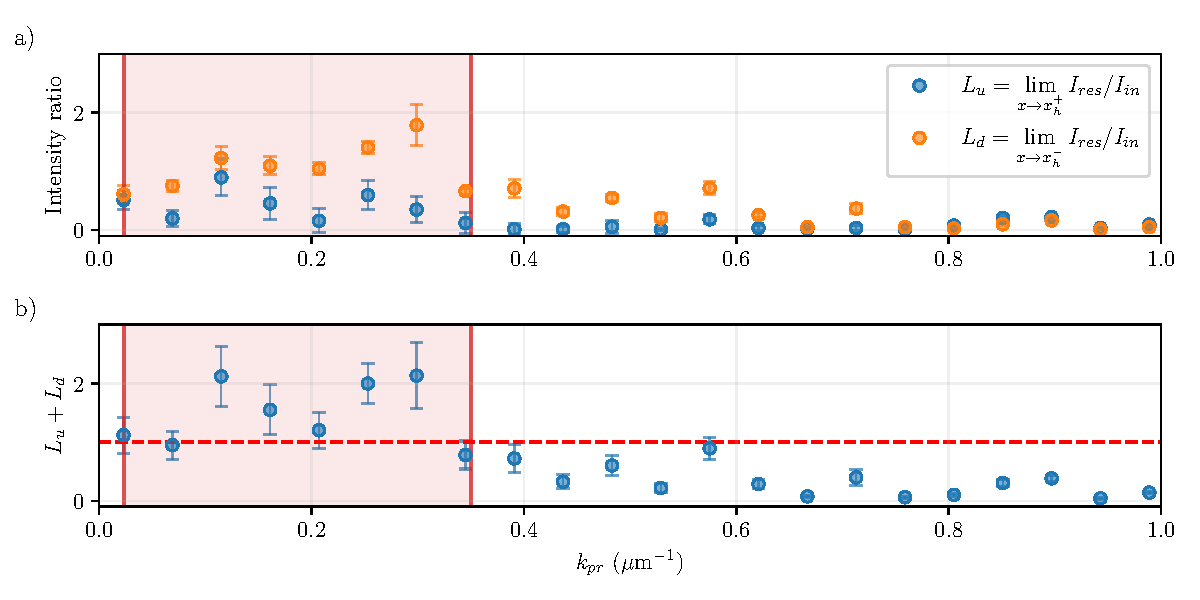
\includegraphics[width=1\textwidth]{chap_stimulated_hawking/fig/I_ratio_bary.pdf}
    \caption{\textbf{a) Intensity ratio.} Estimation of the reflection and transmission coefficients by taking the left and right limits of the intensity ratio $I_{res}/I_{in}$ at the interface. 
    The red colored region corresponds to the probe configurations where stimulated Hawking radiation is expected. The error bars are calculated by taking into account uncertainties on the horizon position as well as the standard deviation of the energy ratio $E_{in}/E_{tot}$.
    \textbf{b) Sum of the reflection and transmission coefficients.} The error bars result from the quadratic sum of the relative error bars on the reflection and transmission coefficients. The red dashed line represent the line $L_u+L_d=1$.}
    \label{fig:I_ratio_bary}
\end{figure}

\bigskip

\textbf{Analysis and discussion.} The first thing to notice is that the left and right limits of the intensity ratio are enhanced when the input mode lies in the negative-positive energy mixing interval as shown in \autoref{fig:I_ratio_bary}. This demonstrates that the contribution of the residual field is larger than in the other configurations and suggests that the scattering process is indeed different in this frequency interval. The sum of these two quantities is shown in \autoref{fig:I_ratio_bary}~\textbf{b)}. As visible,
it can exceed one in the Hawking frequency range.

Together with the measurement of the $d2^*_{out}$ modes presented in \autoref{fig:spectrum_spectro} these results provide a signature of amplification stemming from negative-positive energy mixing at the interface. However, as explained above, these values do not provide a direct measurement of the reflection and transmission coefficients despite all the efforts made to account for the discrepancies introduced by the mode decomposition.
To obtain a quantitative measurement of the scattering coefficients, a better definition of the input modes is needed. Indeed, building the input mode from a Gaussian fit and a linear phase does not take into account the interplay between pumping, propagation and losses. A more accurate estimation would require a complete resolution of the Bogoliubov equation (\ref{eq:bogo_matrix}) by adding a force term to account for the probe laser injection. 

From an experimental point of view, this can be done by placing the probe laser far enough from the interface in the upstream region so it does not interact with it. This would provide
a direct way to compare the field with and without the interface, and any difference could be interpreted as a horizon feature. A second significant 
improvement would be to create a more homogeneous fluid in the unpumped region. This would reduce spurious scattering events and make the plane wave approximation more reliable.
This could be achieved either by finding a working point that is free of cavity impurities or by turning to the geometries created in the previous chapter where the pump intensity is finite everywhere.
Finally, finding a way to measure $d2_{out}^*$ and more generally, all the conjugate modes, with the same powerful interferometric method would allow a more straightforward comparison with the other modes, as well as real space information about their location, amplitude and phase. Implementing this method requires finding a phase reference at the conjugate frequency, which is phase locked with the probe laser. A possible solution would be to create two neighboring fluids with the same lasers, one for the experiment and one to create a reference beam through four-wave mixing. The advantage of this approach is that the reference beam would be naturally phase locked with the probe laser and directly at the conjugate frequency.
Furthermore, having a local oscillator at the ghost branch frequency paves the way to quantum noise measurements such as homodyne detection and squeezing measurements \cite{agullo_symplectic_2022}.



\section{Conclusion}
\label{sec:conclusion}


In this chapter, we have presented the first experimental observation of stimulated Hawking radiation in a polariton quantum fluid. Using a fully optical approach, we demonstrated the ability to reconstruct the fluctuation field and detect scattered modes, providing evidence of negative-positive energy mixing at the interface.
 This mixing, a hallmark of the Hawking effect, was observed through the detection of outgoing modes and the conjugate mode \(d2_{out}^*\), which together suggest amplification.
Our measurement method, based on interferometric techniques, proved to be a powerful tool for isolating and analyzing the scattered modes. This approach highlights the versatility of the polaritonic platform, which, due to its optical nature, is particularly well-suited for such experiments. 
The results presented here pave the way for a more quantitative analysis of the scattering process, including the reconstruction of the scattering matrix. Such a complete measurement would be a significant step forward, enabling the study of correlations between emitted modes and providing deeper insights into the quantum nature of the Hawking effect.
This work once again demonstrates the potential of polariton systems as a platform for exploring fundamental aspects of quantum field theory in curved spacetime. The combination of tunability, out-of-equilibrium properties, and full optical accessibility makes polariton fluids uniquely suited for analog gravity experiments, offering a promising avenue for future studies of quantum effects at analog horizons.
% !TeX encoding = UTF-8
% !TeX spellcheck = fr_FR
% !TeX root = ../mythesis.tex
% !TeX program = pdflatex (build)
%%% TeXmaker : no 'magic comments' but set Root with Options > Set as master file

%useful stuff for what follows

\newcommand{\hf}{\hat{f}}
\newcommand{\hX}{\hat{X}}
\newcommand{\hY}{\hat{Y}}

\graphicspath{{./}{./fig/}{./chap_correlation/fig/}}

\chapter{Bogoliubov modes correlations in polariton quantum fluid}

\label{chap:correlation}

The study of collective excitations in quantum fluids is fundamental to understand nonequilibrium dynamics and many-body interactions. Furthermore, the analog Hawking radiation
on which this work is focused, is expected to create non classical correlations between bogoliubov modes, the event horizon acting as a two mode squeezer \cite{agullo_symplectic_2022}. The simplest manifestation
of paired correlated emission can be observed in the density fluctuations second order correlation function \cite{nguyen_acoustic_2015, carusotto_stimulatedfluid_2016,jacquet_quantum_2023,steinhauer_observation_2016}.
This observable exhibits correlation pattern in the density fluctuations of the fluid on both side of the horizon.
Yet, this has been done only numerically in polaritonic system since the experimental equivalent would require to resolve the polariton lifetime $\sim 10 \mathrm{ps}$. However 
the strong photonic component of this system suggest that correlations between collective excitations modes must have an optical signature that could be adressed
with all the tools developpped in quantum optics.
In this work, we report the first experimental measurement of correlations between collective excitation modes—Bogoliubov modes—in a static and homogeneous quantum fluid of microcavity exciton-polaritons.
 By using a balanced detection set-up, we measure intensity correlation between the normal and ghost branches, probing the fluctuation dynamics of polariton fluids and extracting the spectral correlations of Bogoliubov excitations.
  We observe a clear enhancement of the intensity correlations when the polariton fluid operates near the turning point of the bistabilty due to the emergence of correlated phonon-like excitations. These correlations, seeded by quantum and thermal fluctuations, provide insights into the role of the nonlinear and phononic interactions in the collective excitations of a polariton quantum fluid.

\section{Quantum noise of an electromagnetic field}
\label{sec:intro_cv}
\subsection{Standard quantum limit}
Let us first consider a mode of the electromagnetic field with a frequency $\omega$, quantized within a box of volume V. At a fixed point in space, the electric field can be expressed using the photon creation and annihilation operators :

\begin{equation}
    \label{eq:field}
    \begin{aligned}
    \hat{E}(t) &= E_0\left( \hat{a} e^{-i\omega t} + \hat{a}^{\dagger} e^{i\omega t} \right) \\
    &= E_0\left(\hX\cos (\omega t) + \hY\sin(\omega t)\right)
    \end{aligned}
\end{equation}
where we introduced the quadrature operators $\hX$ and $\hY$ defined as :

\begin{equation}
    \label{eq:quad}
        \hX = (\hat{a} + \hat{a}^{\dagger})  \ \ \mathrm{and}  \ \
        \hY = i(\hat{a}^{\dagger} - \hat{a}).
\end{equation}
The amplitude of the field $E_0=\sqrt{\frac{\hbar \omega}{2\epsilon_0 V}}$ where $\epsilon_0$ is the vacuum permitivity, corresponds to the electric field of a single photon with energy $\hbar \omega$ in the quantization volume $V$. 
For a classical field, $X$ and $Y$ are real numbers and correspond to the real and imaginary parts of the complex field amplitude in the Fresnel representation as visible in \autoref{fig:fresnel} \textbf{a)}. In quantum mechanics,
the quadrature operators are conjugate variables. Indeed, by using the commutation relation of the photon creation and annihilation operators $[\hat{a},\hat{a}^{\dagger}]=1$, we obtain :

\begin{figure}
    \centering
    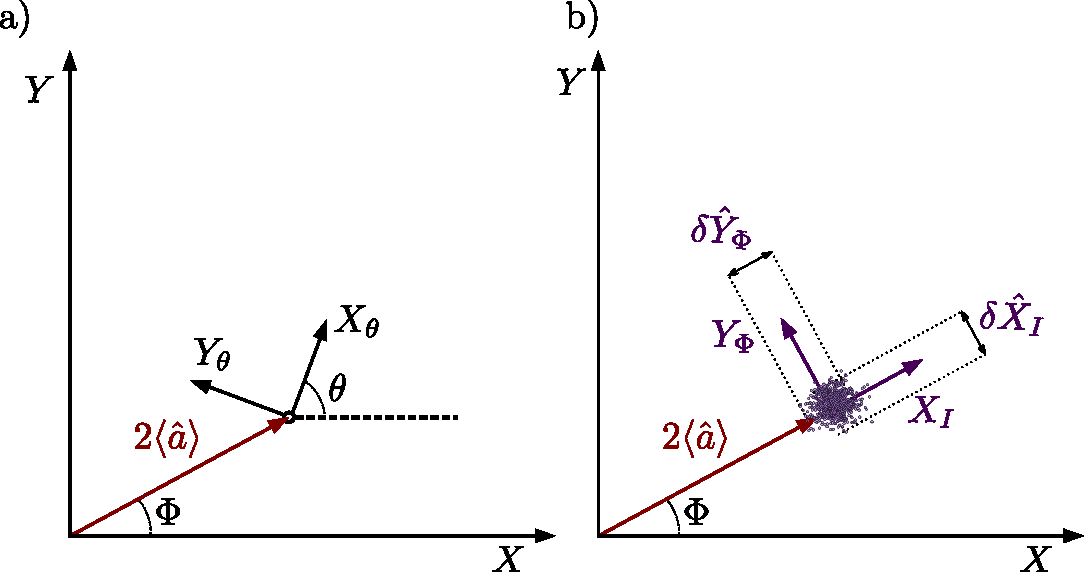
\includegraphics[width=0.8\textwidth]{chap_correlation/fig/fresnel.pdf}
    \caption{ \textbf{a)} Fresnel representation of a classical state. \textbf{b)} Quantum representation 
    of the quadrature operators. The spreaded cloud of points around the mean value $(\langle \hX \rangle, \langle \hY \rangle)$ represents several measurements of the same quantum state. The area of the cloud 
    is bounded from below by the Heisenberg uncertainty principle. The quadratures $\hX_{I}$ and $\hY_{\Phi}$ are the amplitude and phase quadratures respectively.}
    \label{fig:fresnel}
\end{figure}


\begin{equation}
    \label{eq:commut}
    [\hX,\hY] = 2i.
\end{equation}
Consequently, the quadrature operators are non-commuting variables and cannot be simultaneously measured with arbitrary precision. This is a direct consequence of the Heisenberg uncertainty principle stating that the product of the uncertainties in the two quadrature measurements is bounded from below by a constant value.
More precisely, the variances $\Delta X^2 = \langle \hX^2 \rangle - \langle \hX \rangle^2$ and $\Delta Y^2 = \langle \hY^2 \rangle - \langle \hY \rangle^2$ must satisfy the inequality :
\begin{equation}
    \label{eq:uncertainty}
    \Delta X^2 \Delta Y^2 \geq 1
\end{equation}
In contrast with the classical case, the vector $(\langle \hX \rangle, \langle \hY \rangle)$ representing the expectation values of the operators is associated with uncertainties whose area is bounded by the Heisenberg principle. 
The state most closely resembling a classical field is the one in which the fluctuations in both quadratures saturate \autoref{eq:uncertainty}. In this case, the uncertainty area assumes a circular shape with a diameter $E_0$ in the phase space, as illustrated in \autoref{fig:fresnel} \textbf{b)}. In this figure, the field and its fluctuations are not represented on the same scale; a laser field comprises a very large number of photons, whereas the fluctuations are of the order of the field of a single photon. 
Such a minimum uncertainty state is referred to as a coherent state while the corresponding fluctuations define the standard quantum fluctuations. Coherent
state are typically produced by a laser way above threshold and are the eigenvector of the annihilation operator $\hat{a}$.

\subsection{Intensity and phase fluctuations}

The choice of a given set of quadrature operators is arbitrary and corresponds to a choice of phase reference.
Moving to another set of operators $\hX_{\theta},\hY_{\theta}$ consists in a rotation in the phase space :

\begin{equation}
    \hX_{\theta} = \hX \cos(\theta) + \hY \sin(\theta) \ \ \mathrm{and} \ \
    \hY_{\theta} = -\hX \sin(\theta) + \hY \cos(\theta).
\end{equation}

The rotated operators satisfy the same commutation relation \ref{eq:commut} and the uncertainty relation \ref{eq:uncertainty} remains valid. 
However, a particular choice of quadratures is often made in the context of quantum optics \cite{grynberg_aspect_fabre} which consists in
chosing $\theta=\Phi$ where $\Phi$ is the phase of the mean field $\langle \hat{a}\rangle= |\hat{a}|e^{i\Phi}$.  The fluctuations of the corresponding quadrature
operators that we call $\hX_{I}$ and $\hY_{\Phi}$ are then proportionnal to intensity and phase fluctuations respectively as shown in \autoref{fig:fresnel} ~\textbf{b)}. In the case of 
a laser beam, the standard quantum limit is also referred to as the shot noise limit and ultimately originate from spontaneous emission of photons in the gain medium which yields a poissonian statistics in the photon arrival time \cite{grynberg_aspect_fabre}.
Indeed, the measurement of the intensity of a laser beam is subject to statistical noise scalling as the square root of the mean number of photons in the beam.

\begin{equation}
    \label{eq:shotnoise}
    \Delta \hat{N}^2 = \langle \hat{N}\rangle
\end{equation}
From an experimental point of view, this relation is helpfull since it provides a direct way to infer the standard quantum limit from an intensity measurement.   


\subsection{Squeezed states}
While vacuum fluctuations serve as a reference for quantum fluctuations, there is nevertheless no fundamental restriction against obtaining states in which the fluctuations of a given quadrature, $\hX_{\theta}$, are reduced below the standard quantum limit. Indeed, the Heisenberg inequality pertains to the product of uncertainties.
 This inequality remains satisfied provided that the fluctuations in the orthogonal quadrature $\hY_{\theta}$ increase accordingly. Graphically, their representation is obtained by squeezing the uncertainty area along the direction of the quadrature $\hX_{\theta}$ and stretching it along the direction of $\hY_{\theta}$. The resulting states are referred to as a squeezed state, and are of great interest 
 in quantum optics as they can be used to enhance the sensitivity of measurements. As an example, phase squeezed state are used in LIGO-VIRGO infrastrucutres to resolve the infinitesimal displacements of the interferometer mirrors induced by the passing gravitational waves.

\section{Photodectection}
\label{sec:photodetection}


A photodetector is a device that converts the energy of a photon into an electrical signal. The most common type of photodetector is the photodiode, which operates by generating a current in response to the absorption of photons. 
In principle, such devices allows to acquire and process all the information contained in the electromagnetic field by electronic means.
However, an optical field oscillates at hundreds of terahertz, which is far beyond the bandwidth of any electronic device. A photodiode can thus 
only provide a time-averaged signal, which is proportional to the intensity of the field. More precisely, the mean value of the photo-current $\bar{i}$ is proportionnal to the incoming photon flux as :

\begin{equation}
    \label{eq:photocurrent}
    \bar{i} = \eta e \dfrac{P}{\hbar\omega}
\end{equation}
where $\eta$ is the quantum efficiency of the photodetector, $e$ is the electron charge, $P$ is the power of the incoming light and $\hbar\omega$ is the energy of a single photon. 
In the ideal case $\eta=1$ where $100\%$ of the photons are converted into electrons the current statistics reproduce exactly the statistics of the incoming light.
However, in practice, the quantum efficiency is always less than one and the photodetector introduces losses that add to the photonic losses that the incoming beam may has already undergone.
Such losses are random events and subsequently lead any statistics to become Poissonian when they are large enough.


This being said, a incoming photon flux shot noise limited will produce a photocurrent that also follows a Poissonian statistics. For a mean number 
of electron $N_e$ produced by the photodetector, the variance is :

\begin{equation}
    \label{eq:n_e_variance}
    \Delta N_e^2 = N_e.
\end{equation}
From which we deduce the variance of the photocurrent on a time interval $\Delta t$ :
\begin{equation}
    \label{eq:photocurrent_variance}
    \Delta i^2 = \dfrac{e^2\Delta N_e^2}{\Delta t^2}=\dfrac{e^2N_e}{\Delta t^2}.
\end{equation}
Furthermore, by writting $N_e=\bar{i}\Delta t/e$ we obtain :
\begin{equation}
    \label{eq:photocurrent_variance2}
    \Delta i^2 = \dfrac{e\bar{i}}{\Delta t}.
\end{equation}
This relation shows that the variance of the photocurrent is inversely proportional to the time interval over which the current is measured. In the frequency
domain it means that the variance is proportionnal to the bandwidth of the measurement apparatus $\delta f=1/2\Delta t$. 
Furthermore, in the case where the latter can be modeled by a narrow band-pass filter centered on an analysis frequency $\omega_c$ it can be shown \cite{fabre_houches_97}
that the variance of the photocurrent is related to its power spectral density as :

\begin{equation}
    \label{eq:photocurrent_variance3}
    \Delta i^2 = 2\delta f S_i(\omega).
\end{equation}
This is precisely how a spectrum analyzer behaves. It measures the power spectral density of the photocurrent $S_i(\omega)$ by integrating the variance of the current over a given bandwidth $\delta f$ usually limited by the resolution 
bandwith (RBW) of the device.
At the end, we have a way to measure the power spectral density of the incoming light field by measuring the variance of the photocurrent. 
Let us now see how such a device can be used to measure the correlations between two fields.

\section{Balanced detection}

Intensity balanced detection is a common detection scheme used to suppress the classical noise commonly present in optical measurements.
The basic principle of this technique is to use two photodetectors, each measuring the intensity of an optical field, and to subtract their output photo-currents. If the two 
beams share the same classical noise, the subtraction will cancel it out, leaving only the quantum correlations. A representation of the balanced detection scheme is shown in \autoref{fig:balanced_detection}.
Usually, these kind of apparatus are also able to measure the sum of the two photo-currents which is proportional to the total noise of the two beams. However,
as we will see in the next section, measuring the difference together with the individual photo-currents is sufficient to obtain the correlation function of the two fields.
\begin{figure}
    \centering
    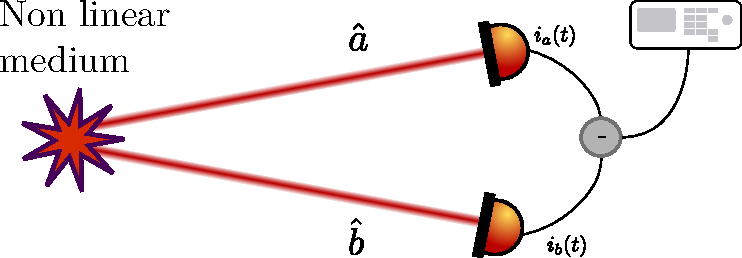
\includegraphics[width=0.8\textwidth]{chap_correlation/fig/balanced_detection.pdf}
    \caption{Balanced detection scheme. Example of a typical non linear medium producing two modes of the electromagnetic field $\hat{a}$ and $\hat{b}$. Each of them is sent to a photodiode that produces a photo-current carrying the noise
    of the beams. The output photo-currents are then subtracted to cancel the classical noise and sent into a spectrum analyzer.}
    \label{fig:balanced_detection}
\end{figure} 

\subsection{Difference measurement}
Let us consider two fields $\hat{a}$ and $\hat{b}$ impinging on two photodetectors as shown in \autoref{fig:balanced_detection}. Their respective intensity 
are given by their number operator $\hat{N}_a=\hat{a}^\dagger\hat{a}$ and $\hat{N}_b=\hat{b}^\dagger\hat{b}$.
We are interested in the intensity difference operator $\hat{N}_-$ defined as :
\begin{equation}
    \label{eq:diff_op}
    \hat{N_-} = \hat{a}^\dagger\hat{a} - \hat{b}^\dagger\hat{b}.
\end{equation}

As explained above, it is convenient to linearize each operator around its mean value :
\begin{equation}
    \begin{aligned}
    \hat{a} &= |\alpha|e^{i\Phi} + \delta \hat{a} \\
    \hat{b} &= |\beta|e^{i\Psi} + \delta \hat{b}
    \end{aligned}
\end{equation}
where $|\alpha|e^{i\Phi}$ and $|\beta|e^{i\Psi}$ are the mean values of the two fields and $\delta \hat{a}$ and $\delta \hat{b}$ are their respective fluctuations.
The difference operator can then be expressed to first order in the fluctuations as :
\begin{equation}
    \label{eq:diff_op2}
    \begin{aligned}
    \hat{N_-} &= (|\alpha|^2e^{i\Phi}+\delta \hat{a}^\dagger)(|\alpha|e^{i\Phi}+\delta \hat{a}) - (|\beta|^2e^{i\Psi}+\delta \hat{b}^\dagger)(|\beta|e^{i\Psi}+\delta \hat{b}) \\
    &= |\alpha|^2 - |\beta|^2 +(|\alpha|\delta \hX_a^\Phi + |\beta|\delta \hX_b^\Psi) 
    \end{aligned}
\end{equation}



\section{Correlations in continuous-variables quantum optics}
\label{sec:corr_cv}
As a very general statement, two quantities are said to be correlated if they ultimately originate from the same source or quantum process. In this case, a knowledge of one of the two quantities gives informations about the other.
Take the example of a two photons emission by a non linear process such as a Type II spontaneous parametric down conversion (SPDC). Their correlations is of several natures. The first and most obvious one is temporal in the sense that the two photons are emitted at the same time. This can be
quantified by looking at the second order intensity correlation function $g^{(2)}(t,t')$, which is the probability of detecting a photon at time $t$ and another one at time $t'$ \cite{hanbury_brown_twiss_1956}. They can also 
be correlated through their polarization meaning that if one photon is detected in a given polarization, the other one will be detected in the orthogonal polarization. Reversing the picture,
the measurement of a given type of correlations can thus provide informations about the quantum nature of the process that generated them.

The question of correlations can also be asked for a field and a version of itself that is delayed in time or shifted in space. In this case, one is in fact looking at the coherence of the field. 
To keep a general descrption let us consider a quantum operator evolving in time $\hat{f}(t)$. The autocorrelation of $\hf$ at time $t$ and $t'$ is defined as :



According to the Bogoliubov theory, this ratio is expected to behave as :

\begin{equation}
    \begin{aligned}
    \dfrac{u_{k_{pr}}^2}{v_{k_{pr}}^2} & \sim \dfrac{\hbar^2k^4}{\mlp^2g^2n_0^2} \mathrm{when \ k_{pr} \ll 1/\xi} \\
    &\sim 
    \end{aligned}
\end{equation}





\begin{equation}
    \label{eq:autocorr}
    C_{\hf}(t,t') = \langle \hf(t)\hf(t') \rangle = \langle \delta \hf(t) \delta \hf(t') \rangle
\end{equation}
where $\delta \hf(t) = \hf(t) - \langle \hf(t) \rangle$ is the fluctuation of the operator around its expectation value. If the process at stake 
is stationary, $\langle \hf(t) \rangle$ does not depend on $t$ and the correlation function depends only on the time difference $\tau= t-t'$ \cite{bachor_guide_1998}. In this case,
the Wiener-Khinchin theorem states that the autocorrelation function is related to the spectral density of the field $\mathcal{S}_{\hf}(\omega)$ by a Fourier transform \cite{fabre_houches_97} :

\begin{equation}
    \label{eq:autocorr_spectral}
    S_{\hf}(\omega) = \int_{-\infty}^{+\infty} C_{\hf}(\tau) e^{-i\omega \tau} d\tau.
\end{equation}

In the same manner it is possible to define the cross-correlation between two operators $\hf_1$ and $\hf_2$ as :

\begin{equation}
    \label{eq:crosscorr}
    C_{\hf_1,\hf_2}(t,t') = \langle \hf_1(t)\hf_2(t') \rangle = \langle \delta \hf_1(t) \delta \hf_2(t') \rangle
\end{equation}

\section{Experimental implementation}
\label{sec:exp_impl}




The set up used is similar to the one used in the previous experiement with the addition of a balanced detection scheme that will be detailled in the next section. 
The microcavity is the same as the one used in the previous chapters but the experiment is runned at the working point B10-C10 (see ?????).

\bigskip

\subsection{Bogoliubov coefficients measurement}


\textbf{Mean field} We create a static polariton fluid by shinning a pump laser beam of diameter $w=\SI{100}{\micro\meter}$ at normal incidence on the microcavity ie at $k_p=0$. The laser is detuned from the polariton resonance by
$\delta = \SI{35}{\giga\hertz}$ in order to operate in a bistable regime. The pump laser is $\sigma_+$ polarized in order to excite a single polariton population \cite{timofeev_exciton_2012}. A typical real space image of the polariton fluid is shown in \autoref{fig:real_space} \textbf{a)}. 


\begin{figure}
    \centering
    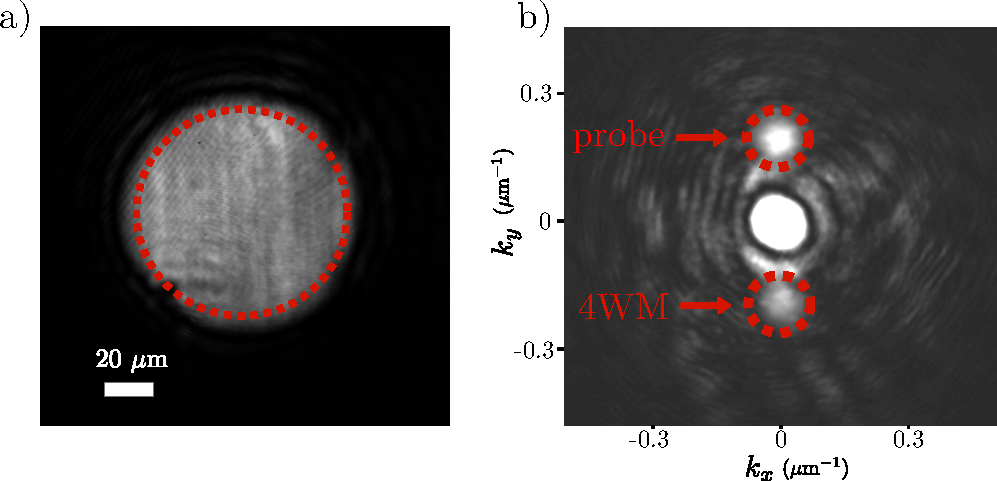
\includegraphics[width=1\textwidth]{chap_correlation/fig/r_and_k_space.pdf}
    \caption{\textbf{a)} Real space image of a polariton fluid operating on the high density branch of the bistability loop. The image is taken at the working point B10-C10. The red dashed circle represents
    the pinhole applied to the image to filter out the signal coming from the edges of the fluid. \textbf{b)} Corresponding k-space image of the polariton fluid when a weak probe is exciting the normal branch at $k_{pr}=\SI{0.2}{\per\micro\meter}$. 
    The direct transmission of the probe is pointed out by the red arrow on top of the image while its four wave mixing signal is visible at $-k_{pr}$. The red dasehd circles represent the pinholes applied 
    in the fourier plane to isolate each signal before sending it to the balanced detection scheme. }
    \label{fig:real_space}
\end{figure}


\bigskip

To begin with, the collective excitation spectrum of the fluid is measured with the same method than in \autoref{chap:generation_transonic_fluid}. The pump laser intensity is set to operate close to the turning point of the higher branch of the bistability loop but sufficiently  fro from it to have a stable polariton fluid. 
We don't aim at 
The normal branch shown in \autoref{fig:uv_analysis} \textbf{a)} is measured through direct excitation ie by placing pinholes that track the probe wavevector in the fourier space at each energy scan.
 Conversely, the ghost branch shown in \textbf{b)} is measured through 4WM excitation meaning that the pinholes are systematically positioned at the opposited wavevector $-k_{pr}$. At each couple $(k,\omega)$ and $(-k, -\omega)$ the corresponding intensities are measured by fitting the resonance peaks 
by a Lorentzian function. As outlined by the previous section, when the probe is resonant with a normal branch Bogoliubov mode at $(k_{pr}, \omega_{pr}=\ombog^+(k_{pr}))$ the expected emission intensities in each branch are given by :

\begin{equation}
    \label{eq:uv_intensity}
    \begin{aligned}
    I_N(k_p, \omega_{pr}) &= |u_{k_{pr}}|^4 |\alpha|^2  \  \mathrm{for \ the \ normal \ branch } \\
    I_G(-k_p, -\omega_{pr}) &= |v_{k_{pr}}u_{k_{pr}}|^2 |\alpha|^2 \ \mathrm{ for \ the \ ghost \  branch,}
    \end{aligned}
\end{equation}
with $|\alpha|^2$ the intracavity probe intensity. By then measuring the ratio of the two quantities, the probe contribution disappears and we can have acces to the Bogoliubov coefficients ratio $u_{k_{pr}}^2/v_{k_{pr}}^2$. 
\autoref{fig:uv_analysis} \textbf{c)} shows this ratio as a function of the probe wavevector $k_{pr}$. At low wavevector, the ratio tends to a constant value which is expected from the Bogoliubov theory as explained in the previous section. A quantitative value of this value can non be extracted from the data
because at low wavevector the measurement method does not allow to discriminate the two conjugated modes. However, one can appreciate that the ratio is close to one which is consistent with the theoretical prediction.
At high wavevector $u_{k_{pr}}^2/v_{k_{pr}}^2$ is expect to follow a $k^4$ law as previously explained. To discuss this feature, we take the data for $|k_{pr}| > 1/\xi\approx\SI{0.35}{\per\micro\meter}$ and fit them with a power law of the form $ak^\beta$ with $a$ and $\beta$ as fitting parameter. The healing length $\xi=\SI{3}{\micro\meter}$ is estimated from the detuning $\delta =\SI{35}{\giga\hertz}$ which is slightly lower than the interaction energy $gn_0$ since the system operates close to the turning point of the bistability loop.

\bigskip

The resulting fit are represented by the red dashed line in \autoref{fig:uv_analysis} \textbf{c)}. The fit gives a value of $\beta=3.74\pm0.5$ for negative wavevector whereas for positive wavevector we obtain $\beta=1.47\pm{0.5}$. The first value is consistent with the Bogoliubov theory prediction of $\beta=4$ while the second one is not. The uncertainty on $\beta$ is of $16\%$ for $k<0$ and $34\%$ for $k>0$. Despite the fact this suggests that 
the fit is better for negative wavevector, the uncertainty is too large in both cases to draw a quantitative conclusion on the Bogoliubov coefficients ratio. This asymetry between the two branches is not well understood and may be due to a sample effect that is not perfectly istropic. Indeed, 
as explained in \autoref{chap:generation_transonic_fluid}, the sample exhibits a so called wedge which can be understood as a small tilt of the microcavity DBR mirrors. This creates a direction along which the photon resonance energy increases as a function of the cavity width.
This breaking of symmetry may result in a $k$-dependent efficiency of the emission that is not taken into account in the initial model. A way to verify this hypothesis would be to precisely characterize the wedge as well as the $k$-dependance of the DBR reflectivity and run numerical simulations of angle and energy resolved emission. 

With that being said, it is worth noticing that at low wavevector $|k_{pr}|<\SI{0.5}{\per\micro\meter}$ where $k$ and $-k$ are closer to each other, symmetry between the branch is restored which support the anisotropy hypothesis 
we just made.

\bigskip

\textbf{Bogoliubov coefficients.} The Bogoliubov coefficients $u_{k_{pr}}$ and $v_{k_{pr}}$ can be separately extracted from the ratio $u^2/v^2$ by using the normalization condition $u^2-v^2=1$. The 
results are shown in \autoref{fig:uv_analysis} \textbf{d)}. While we observe a clear enhancement of both coefficients at low wavevector, we do not observe the $1/k$ divergence expected from the Bogoliubov theory. This is not due to the incapacity of the experimental method to disitinguish the modes a low wavevector since 
such a divergence should be observed in the overall intensity.
In fact, in the litterature \cite{pitaevskij_bose-einstein_2016,castin_bose-einstein_2001,pethick_bose-einstein_2008}, this $1/k$ behavior is computed for a homogeneous and infinite condensate. In practice, eventhough the polariton fluid is homogeneous it has a finite size of $w=\SI{100}{\micro\meter}$. The latter,
limits the minimum wavevector that can be probed to $k_{min}=\pi/w\approx\SI{0.03}{\per\micro\meter}$. In other words, it is not possible to excite modes that correspond to interactions ranges greater than the size of the fluid.

In view of measuring correlation between the bogoliubov modes, the fact that the emissions in the two branches become balanced at low wavevector suggests that correlations should increase in this regime \cite{treps_fabre_criteria_2004}. This is precisely what we observe as we will see in the next section.


\begin{figure}
    \centering
    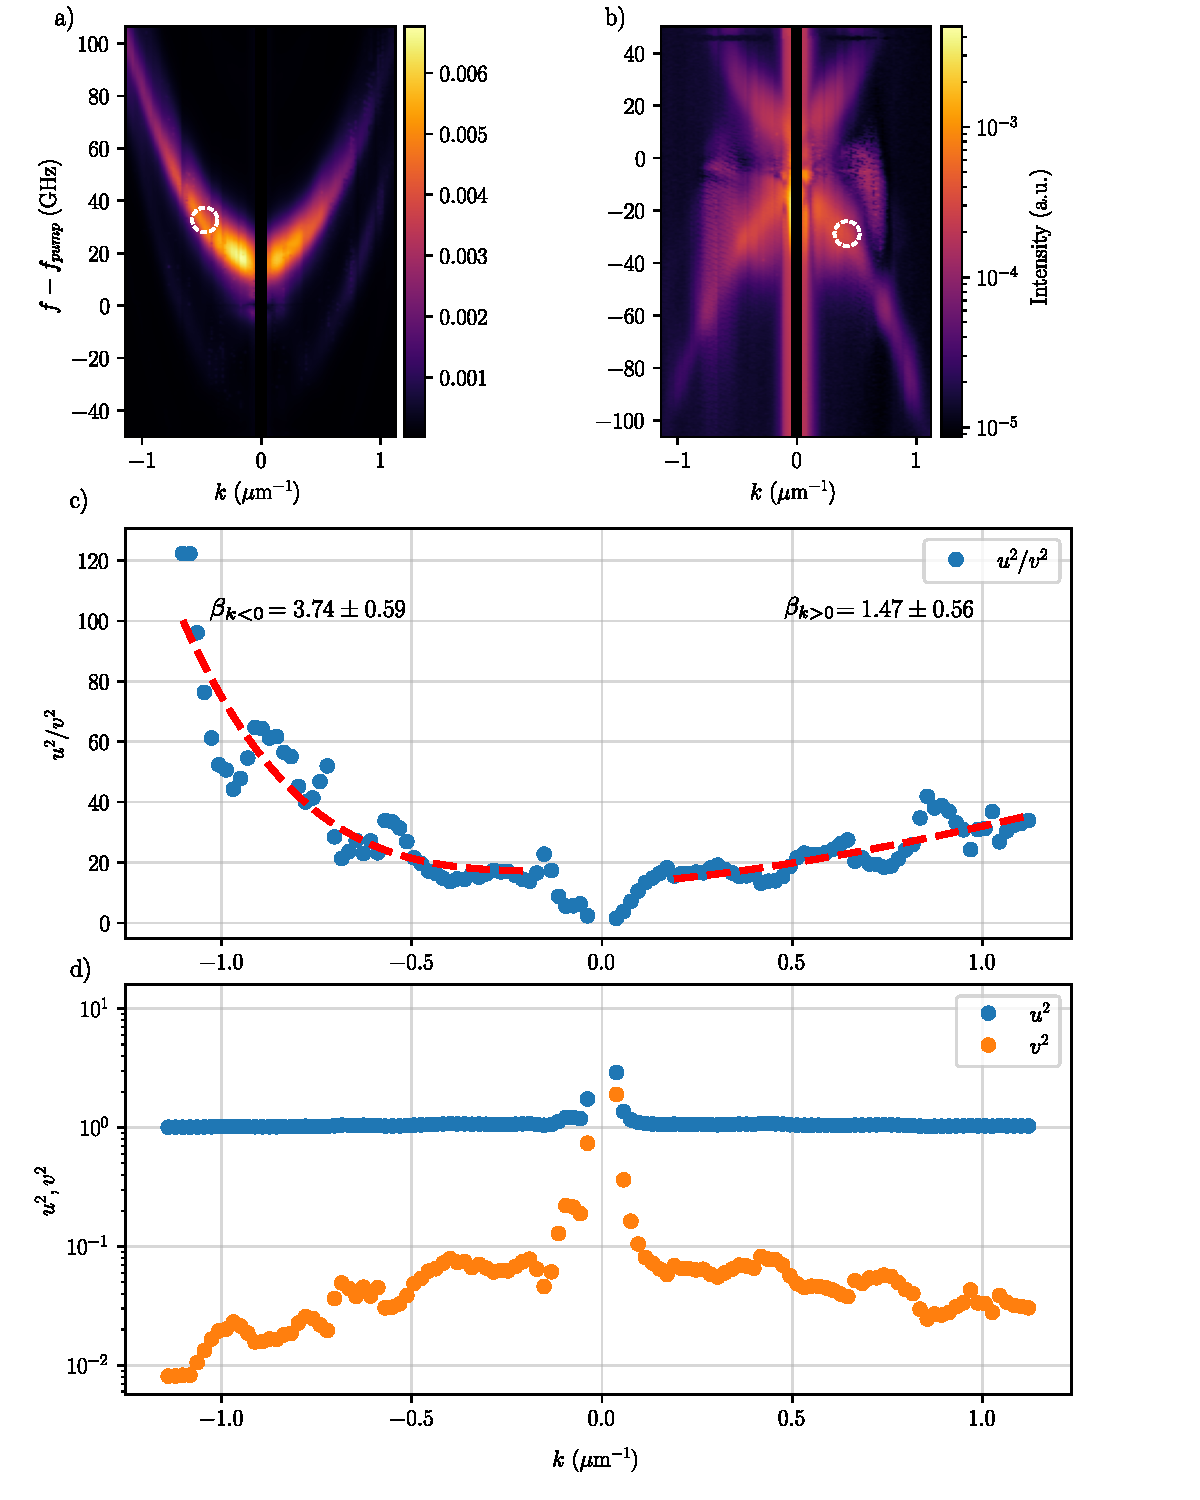
\includegraphics[width=1\textwidth]{chap_correlation/fig/uv_analysis.pdf}
    \caption{\textbf{Bogoliubov dispersion measurement.} \textbf{a)} Normal branch measurment. \textbf{b)} Ghost branch measurement. As explained in \autoref{chap:generation_transonic_fluid}, the black solid rectangle
    centered at $k=0$ on both plots reprents the region where the two conjugated modes start to overlap in the $k$-space and thus cannot be resolved. The white dashed circles represent two conjuagted bogoliubov modes whose emission are compared to exctract the Bogoliubov coefficivents $u$ and $v$.}
    \label{fig:uv_analysis}
\end{figure} 

\subsection{Bogoliubov modes correlations}
\label{sec:exp_corr}


\subsubsection{Shot noise calibration}
Since we are interested in measuring correlations produced by the non linear four wave mixing process, it is necessary to make sure that both of the laser
injected in the microcavity don't introduce any classical noise in the system. Indeed, as explained in \cite{treps_fabre_criteria_2004}, if the laser used to stimulate non linear effect carry classical noise, both of the emitted beam 
will be classically correlated which will result in a strong noise reduction in the difference photocurrent and artificially enhance the correlations.
To verify that the lasers are shot noise limited, we send one of them on a half wave plate followed by polarizing beam splitter (PBS). This enable to precisely balance the two outputs of the PBS before sending them to the balanced detection scheme and make sure 
that any classical noise is cancelled out. Then the intensity of the laser is ramped up. At each intensity value, the power spectral density is measured by a spectrum analyzer in order to determine the linear relation between 
the laser power and the intensity variance. Since all the classical noise has been removed, this variance reflects the poissonian statistics stemming from the intrinsic quantum noise of the lasers as explained in the previous section. As this statistic is universal,
there is no need to make the measurement for the two lasers and the linear coefficient relating intensity and noise is fixed by the measurement apparatus \cite{bachor_guide_1998}.

\begin{figure}
    \centering
    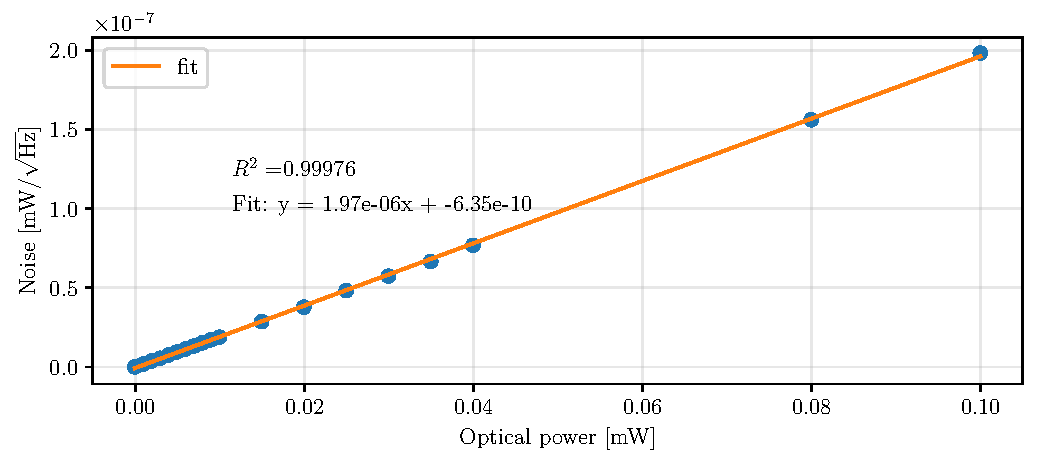
\includegraphics[width=1\textwidth]{chap_correlation/fig/noise_vs_optical_power.pdf}
    \caption{Shot noise calibration. The variance of the photocurrent is measured as a function of the laser power. The dark noise of the apparatus measurement has been substracted. The linear fit excplicit the coefficient relating the intentity of the laser and its intrinsic quantum noise.}
    \label{fig:calibration}
\end{figure}

The results are presented in \autoref{fig:calibration}.
As expected, the variance of the photocurrent is linear with the laser power. This calibration curve is then used to make sure that the lasers are shot noise limited by verifying that, for a given laser power 
its power spectral density falls on the calibration curve. Of course, the settings of the spectrum analyzer as well as the photodetector must be exactly the same as the ones used for the calibration process. Since the quantum noise 
is a white noise, the calibration as well as the experiment can be in principle done at any frequency. However, it is convenient to chose an analysis frequency at least in the MHz range to avoid classical noises like vibrations while staying in the photodetector bandwidth of few MHz. These vibrations are mainly due to the vacuum pump connected to the cryostat an whose 
frequency don't exceed hundreds of kilohertz. Further increasing the analysis mean that the photodetector bandwith must be accordingly increased which would result in a reduction of the apparatus gain and thus of the signal to noise ratio.
To have the best compromise between these constraints, the calibration and the experiment were done at $\SI{1.5}{\mega\hertz}$. 
 


The photodiodes used in this experiment are industrial Thorlabs PDB450A photodiodes with adjustable gain. The latter is set to $10^4$ in order to have a bandwith of $\SI{4}{\mega\hertz}$.
The spectrum analyzer is a RIGOL DSA-815 in zero span mode at $\SI{1.5}{\mega\hertz}$. The resolution bandwidth (RBW) as well as the video bandwidth (VBW) are set to $\SI{100}{\kilo\hertz}$ in order to have a good compromise between the signal to noise ratio and the measurement time.
The sweep time is set to $\SI{100}{\milli\second}$.


\begin{figure}
    \centering
    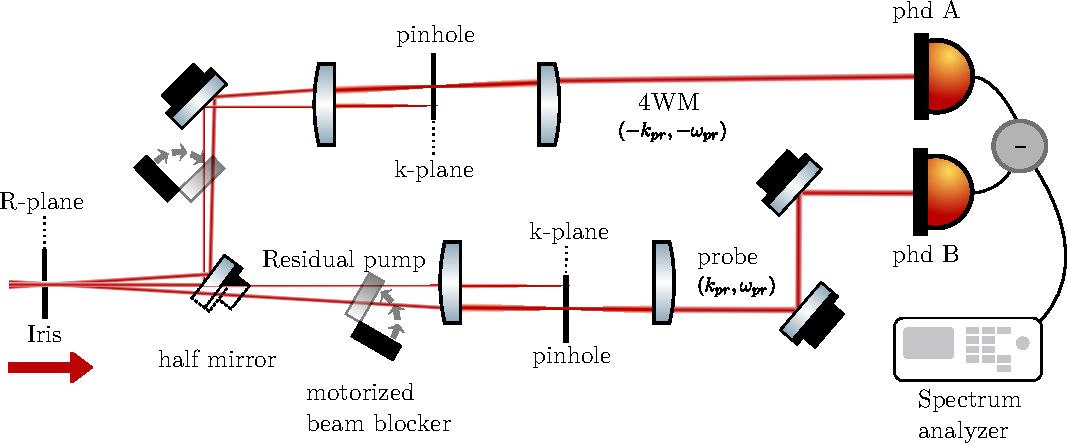
\includegraphics[width=1\textwidth]{chap_correlation/fig/half_mirror.pdf}
    \caption{Experimental set up used to measure the correlations between Bogoliubov modes. The red arrow represent the propagation direction of the light.
    The first real space filtering is done with an adjutable iris diaphragm while the filterings in Fourier space are done with pinholes of diameter $w=\SI{300}{\micro\meter}$ to match the size of the 
    probe. A motorized beam blocker is placed on each optical path to measure the noise of each beam separately. The focal lenghts of the lenses are chosen to magnify the image so its matches the size of the photodiodes sensors that are $d=\SI{800}{\micro\meter}$ in diameter. The two photodiodes are connected to a spectrum analyzer in zero span mode at $\SI{1.5}{\mega\hertz}$. The resolution bandwidth (RBW) and the video bandwidth (VBW) are set to $\SI{100}{\kilo\hertz}$.}
    \label{fig:set_up_balanced}
\end{figure}

\subsubsection{Balanced detection}
Once the polariton fluid is established, we fix the probe wavevector to $k_{pr}=\SI{0.2}{\per\micro\meter}$ and tune the laser frequency to be resonant with the normal branch of the bogoliubov dispersion. The outgoing field from the microcavity is then directed to a balanced detection setup, illustrated in \autoref{fig:set_up_balanced}.
To measure the correlations between the Bogoliubov modes, it is essential to isolate the two conjugated modes from each other but also from the mean field. 

\bigskip

\indent Indeed, if the photodiodes collect residual light from the mean field, the detection scheme may yield a spurious non-zero correlation even in the absence of the probe. Indeed, although the pump laser generating the mean field is shot-noise limited, the photonic component of the polariton fluid escaping the microcavity is not.
This excess noise originates from the Kerr effect inside the cavity, which leads to self-phase modulation of the polariton field. As a result, additional intensity and phase fluctuations are introduced in the fluid. If one spatially isolate two region of the fluid, the fluctuations in the mean field will be correlated, leading to a non-zero correlation signal in the balanced detection scheme.
However, these correlations do not stem from the nonlinear scattering process under investigation, but rather from the monomode character of the polariton fluid as demonstrated in \cite{a_baas_quantum_degeneracy2006}.

\bigskip

\indent To prevent this, we first proceed to a filtering of the polariton fluid in real space as shown in \autoref{fig:set_up_balanced}. The real space image of the polariton fluid is filtered using a pinhole of diameter $w=\SI{100}{\micro\meter}$, which is the same as the pump beam diameter.
The purpose of this filtering is to remove the light coming from the edges of the polariton fluid, which, as explained in the previous chapter, expels polaritons at high momentum and may yield a spurious signal in the detection scheme.
The filtered image is then let to propagate so that the Bogoliubov signals at $k_{pr}$ and $-k_{pr}$ as well as the mean field at $k=0$ are spatially separated in far field. Then, a half mirror is used to split the light into two paths as shown in \autoref{fig:set_up_balanced}.
At this stage, both paths still contain mean field photons. To remove them, another filtering is applied in the Fourier plane to isolate the Bogoliubov modes as shown in \autoref{fig:real_space} \textbf{b)}. This picture shows the whole $k$-space image for the sake of clarity, but in practice,
the top and bottom halves belong to two different paths of the balanced detection scheme.


\begin{figure}
    \centering
    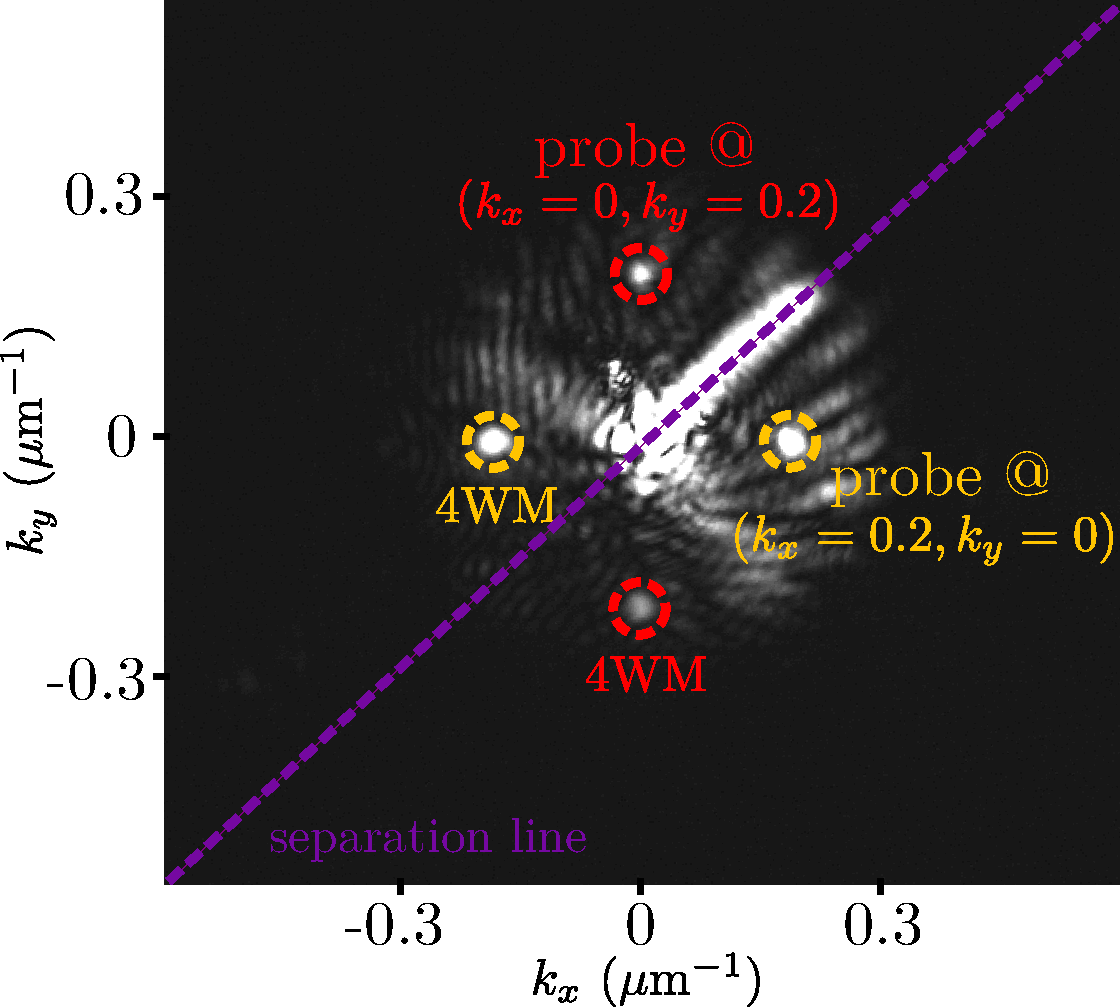
\includegraphics[width=0.5\textwidth]{chap_correlation/fig/mosaic_4wm.pdf}
    \caption{\textbf{Fourier plane of the field with two probe beams injected in the system}. The two beams are injected at $k_{pr}=(0.2,0)$ and $k_{pr}=(0,0.2)$. The red dashed circle represent the conjuagte mode along the $y$-axis and the yellow dashed circles the modes along the $x$-direction. The half mirror is rotated by 45° to separate the top left and right bottom part of the field
    which is represented by the purple dashed line. The pinholes are placed in the Fourier plane at the appropriate wavevector to measure the correlations between two conjugate modes or between two modes that are not conjugate.}
    \label{fig:sanity_check}
\end{figure}

\bigskip

\indent \textbf{Sanity check.} To validate that the apparatus is able to measure correlations between the Bogoliubov modes and is not only measuring the monomode character of the polariton fluid \cite{a_baas_quantum_degeneracy2006}, we inject two probe beams in the system in order to generate two independent 
four wave mixing processs. Both of them come from the same laser : one has a non zero wavevector along the $x$-axis $(k_x=0.2, k_y=0)$ while the other one has a non zero wavevector along the $y$-axis $(k_x=0, k_y=0.2)$. For the sake of clarity we label $k_{x,y}$ the modes directly excited by the probe and $k_{x,y}^*$ their conjugate counterpart. The energy of the laser is again set to be resonant with the normal branch of the Bogoliubov dispersion.
Each of the two probe beams generates its own conjugate mode at its respective opposite wavevector as shown in \autoref{fig:sanity_check}. 
One can notice that the modes along the $y$-axis are less intense than these along $x$ despite the input size and intensity of the two beam is the same. This once again supports the idea that the emission efficiency in one mode or the other is $k$-dependent. 

The verification consists in measuring the correlations between two conjuagte modes and compare it to the correlation between two modes that are not.
If the measurement is dominated by pump contributions one should measure the same result for both cases. To do so, we rotate the half mirror by 45° around its normal axis in order to separate the top left part of the field from the bottom right part and send them to the two optical paths. The separation is explicited
by the diagonal purple dashed line in \autoref{fig:sanity_check}. Then, depending on which couple we want to measure the correlations, we place the pinholes in the Fourier plane at the appropriate wavevector.
The results are shown in \autoref{fig:noise_comparison}. The panel \textbf{a)} displays the power spectral density of the photocurrent difference for the two conjugate modes $k_x$ and $k_x^*$ while \textbf{b)} shows the same measurement for the two modes $k_y$ and $k_y^*$. 
A simple way to infer if the beams are correlated is to compare the difference PSD to the sum of the individual PSDs as if they were not correlated. As visible, in the first case \textbf{a)}, the difference PSD is below the sum of the individual PSDs, which indicates that the two modes are correlated. In contrast, in the second case \textbf{b)}, the difference PSD is superimposed to the sum of the individual PSDs, which indicates that the two modes are not correlated. 

More precisely, we measure a correlation coefficient $C_{k_x,k_x^*}=0.11\pm{0.01}$ for the first case and $C_{k_x,k_y^*}=0.01\pm{0.005}$ for the second one. The error bars are estimated from the standard deviation of the PSDs over the swipe time of the spectrum analyzer.
This result confirms that modes originating from the same four wave mixing process are correlated while modes originating from different processes are not and that the measurement is 
not dominated mean field contributions.

Without loss of generality, note however that this measurement was not done on the same fluid and the same day as the rest of the experiment since the goal was just to provide a proof of principle.  

\begin{figure}
    \centering
    \includegraphics[width=1\textwidth]{chap_correlation/fig/noise_comparison.pdf}
    \caption{Sanity check correlation measurement. \textbf{a)} Power spectral density of the photocurrent difference for two conjugate modes $k_x$ and $k_x*$. \textbf{b)} Power spectral density of the photocurrent difference for two modes that are not conjuated $k_x$ and $k_y^*$. To smooth 
    the date is noise is averaged on 10 sweeps of the spectrum analyzer. In both panels, the red dashed line represents the sum of the two individual photocurrent power spectral density as if they were not correlated. The black dashed line is the dark electronic noise of the apparatus.} 
    \label{fig:noise_comparison}
\end{figure}



\subsubsection{Correlations measurement}
\label{sec:exp_corr_measurement}

The previous section showed that the efficiency of the emission in a given mode appear to be $k$-dependent. As a consequence, studying correlations for different probe wavevectors might not be the best way to investigate the Bogoliubov modes correlations.
Instead, we propose to focus on the correlations as a function of the operating point of the polariton fluid on the higher branch of the bistability loop. 

To do so, we fix the probe wavevector to $k_{pr}=\SI{0.2}{\per\micro\meter}$ and set the pump intensity to operate on the high density branch of the hysteresis curve. Then the pump power is ramped down toward the turning point of the bistability loop.
In terms of collective excitation, the system goes from a parabolic gapped dispersion to a linear gapless one as explained in \autoref{chap:generation_transonic_fluid}.

At each pump power, the probe frequency is tuned to stay resonant with the normal branch Bogoliubov mode at $k_{pr}$. The correlations between the two conjuate mode are then measured the same way as in the previous section. 


% !TeX encoding = UTF-8
% !TeX spellcheck = fr_FR
% !TeX root = ../mythesis.tex
% !TeX program = pdflatex (build)
%%% TeXmaker : no 'magic comments' but set Root with Options > Set as master file

%useful stuff for what follows

\chapter{Conclusion}

In this thesis, we have explored the physics of microcavity polaritons and their application to analog gravity, with a particular focus on the Hawking effect in polariton quantum fluids. By combining theoretical and experimental approaches, we have demonstrated the versatility of this platform for studying curved spacetime and analog gravity effects.

We began by presenting the microcavity polariton system, detailing its unique properties as a hybrid light-matter quasiparticle. This was followed by a theoretical investigation of the Hawking effect in polariton quantum fluids, where we showed how the Bogoliubov excitations in these systems can mimic the behavior of quantum fields in curved spacetime. This theoretical framework provided the foundation for designing experiments to study analog gravity effects.

A key achievement of this work was the demonstration of the tunability of polariton systems, which allowed us to effectively create curved spacetime geometries. By carefully controlling the system parameters, we were able to engineer conditions that emulate event horizons and study the associated analog gravity phenomena. This tunability highlights the potential of polariton systems as a flexible platform for exploring a wide range of analog gravity effects.

We then reported the first observation of stimulated Hawking radiation in a polariton quantum fluid. By injecting a weak probe beam, we stimulated the emission of Bogoliubov modes and observed their properties, providing direct evidence of the analog Hawking effect in this system. This result represents a significant step forward in the experimental study of analog gravity.

Finally, we focused on the measurement of correlations between Bogoliubov modes. By analyzing the intensity correlations, we gained insights into the underlying quantum processes driving the analog Hawking effect. This work paves the way toward the measurement of quantum correlations between modes emitted by an analog horizon, a crucial step for exploring the quantum nature of analog gravity phenomena.

In conclusion, this thesis has demonstrated the potential of microcavity polariton systems as a platform for studying analog gravity and quantum field theory in curved spacetime. The results presented here open new avenues for investigating quantum correlations and non-classical effects in analog horizons, bridging the gap between condensed matter physics and fundamental questions in quantum gravity.
\appendix
\graphicspath{{./}{./fig/}{./appendices/fig0/}}

\chapter{Mean field shaping and monitoring}\label{chap:appendices}


\section{Phase printing}
\label{app:phase_printing}
Controlling precisely the phase of a laser beam is a common but challenging task in optics. The most basic way to do it is by applying spatial filtering in the fourier plane of a lens.
The phase of the beam after a second collimating lens is then given by the covolution product of the beam phase and the mask inverse fourier transform. This method then show its limits when one wants to 
generate complex phase profile since its depend on the mask form. A way to overcome this problem is the use of Digital Micromirror Device (DMD) which is an array of micro-mirrors that can be individually controlled to reflect the light or not.
By putting this array in the fourier plan of a lens it is possible to create spatial filtering with arbitrary shapes. However, this method suffers from high losses and diffraction of the light on the individual mirrors that tend to 
add unwanted noise. This being said, DMD are very powerfull devices and allow to do a great amount of things at low cost. A wide range of possible methods are referenced in the great work \cite{wavefront_shapping}. 

\bigskip

\subsection{Spatial light modulator.} In this work, we use a Spatial Light Modulator (SLM) which is a liquid crystal display that can be used to modulate the phase of a laser beam. The principle is to apply a voltage on each pixel of the SLM to change the orientation of the liquid crystal molecules. 
The phase shift is then given by the difference of the optical path of light going through the different pixels as shown in \autoref{fig:SLM}. 

\begin{figure}
    \centering
    \includegraphics[width=1\textwidth]{appendices/fig0/SLMprinciple.png}
    \caption{Principle of a Spatial Light Modulator.}
    \label{fig:SLM}
\end{figure}

\noindent By shinning a flat phase collimated beam on the SLM which displays the target phase profile the beam gets reflected carrying the desired wavefront.
However the efficiency of the SLM is not perfect and whenever light is shone on it, some photons migth not see it and not be phase modulated. To overcome this difficulty,
we first write a blazed phase grating on the SLM screen on top of which the wanted profile is set. All the photons that did interact with the liquid crystals are then mostly diffracted on the first order of the grating. Doing so,
an efficiency of 60-70\% can be reached. This contrast with the usual 80\% usually claimed on manufacturer datasheets that actually correspond to the efficiency in all orders. A typical phase profile encoded on the SLM is shown
in \autoref{fig:SLM_profile}. A gray value of zero correspond to no shift while 255 corresponds to $2\pi$. The gray map corresponding to the target phase profile has been unwrapped for the sake 
of clarity and is shown in \autoref{fig:SLM_profile} c). The final gray map displayed on the SLM screen in represented in \autoref{fig:SLM_profile} e). 

\begin{figure}
    \centering
    \hspace{-1.4cm}
    \includegraphics[width=1.1\textwidth]{appendices/fig0/slm_typical.pdf}
    \caption{Typical profile encoded on the SLM to generate the target velocity profile. a) Gray map of a phase blazed grating encoded on the SLM screen and b) corresponding cut in the 
    $x$ direction. c) Unwrapped grey map of the target phase profile and d) corresponding cut in the $x$ direction. e) Final gray map encoded on the SLM screen and f) corresponding cut in the $x$ direction. This map is the sum 
    of the blazed grating and the target phase profile modulus 255.} 
    \label{fig:SLM_profile}
\end{figure}

To imprint precisely the resulting wavefront in the cavity plane two $2f-2f$ optical telescopes are used in series to image the SLM screen with an overall demagnification of 1/130 while avoiding short focal lenght that would introduce optical aberrations.
An adjustable slit is placed in the fourier plane of the first telescope to filter out the unwanted diffracted orders.

\subsection{Phase measurement}
\label{sec:phase_measurement}

\subsection{Off axis inteferometry}
The principle is the following :
the beam whose phase is to be measured is recombined on a CCD camera with a flat phase reference beam. An angle is volontary introduced between the two beam to create an interference pattern on the camera plane. The phase difference between 
the two beams is then encoded in the size of the fringes and can be recovered by performing a fourier transform on the interferogram and demodulate the signal around the satellite peak created by the angle between the two beams \cite{liebling_complex-wave_2004}.

\subsection{Controlling the local intensity}

\label{sec:local_intensity}



% % !TeX encoding = UTF-8
% !TeX spellcheck = fr_FR
% !TeX root = ../mythesis.tex
% !TeX program = pdflatex (build)
%%% TeXmaker : no 'magic comments' but set Root with Options > Set as master file

\graphicspath{{./}{./fig/}{./appendices/fig/}}

%%% This chapter (5--10 pages) is required when the main text is written in foreign language


\chapter{Résumé long en français}

\begin{otherlanguage}{french}

Texte du résumé\ldots

\end{otherlanguage}
% Appendice avec un lexique des méthodes expérimentales. 
% Ex : - N2
%      - Phase
%      - SLM stuff etc ...


%%%%%%%%%%%%%% les pages finales %%%%%%%%%%%%%%%%
\backmatter
%\nocite{*} %%% pour les test, mais à proscrire en production
%%% utilisation de BiBTeX
\cleardoublepage
\setlength{\bibhang}{2em}
\raggedright
\bibliography{Quantum_optics_lkb}

\csuse{backcover}
\end{document}